% Options for packages loaded elsewhere
\PassOptionsToPackage{unicode}{hyperref}
\PassOptionsToPackage{hyphens}{url}
\PassOptionsToPackage{dvipsnames,svgnames,x11names}{xcolor}
%
\documentclass[
  letterpaper,
]{krantz}

\usepackage{amsmath,amssymb}
\usepackage{lmodern}
\usepackage{iftex}
\ifPDFTeX
  \usepackage[T1]{fontenc}
  \usepackage[utf8]{inputenc}
  \usepackage{textcomp} % provide euro and other symbols
\else % if luatex or xetex
  \usepackage{unicode-math}
  \defaultfontfeatures{Scale=MatchLowercase}
  \defaultfontfeatures[\rmfamily]{Ligatures=TeX,Scale=1}
\fi
% Use upquote if available, for straight quotes in verbatim environments
\IfFileExists{upquote.sty}{\usepackage{upquote}}{}
\IfFileExists{microtype.sty}{% use microtype if available
  \usepackage[]{microtype}
  \UseMicrotypeSet[protrusion]{basicmath} % disable protrusion for tt fonts
}{}
\makeatletter
\@ifundefined{KOMAClassName}{% if non-KOMA class
  \IfFileExists{parskip.sty}{%
    \usepackage{parskip}
  }{% else
    \setlength{\parindent}{0pt}
    \setlength{\parskip}{6pt plus 2pt minus 1pt}}
}{% if KOMA class
  \KOMAoptions{parskip=half}}
\makeatother
\usepackage{xcolor}
\setlength{\emergencystretch}{3em} % prevent overfull lines
\setcounter{secnumdepth}{5}
% Make \paragraph and \subparagraph free-standing
\ifx\paragraph\undefined\else
  \let\oldparagraph\paragraph
  \renewcommand{\paragraph}[1]{\oldparagraph{#1}\mbox{}}
\fi
\ifx\subparagraph\undefined\else
  \let\oldsubparagraph\subparagraph
  \renewcommand{\subparagraph}[1]{\oldsubparagraph{#1}\mbox{}}
\fi

\usepackage{color}
\usepackage{fancyvrb}
\newcommand{\VerbBar}{|}
\newcommand{\VERB}{\Verb[commandchars=\\\{\}]}
\DefineVerbatimEnvironment{Highlighting}{Verbatim}{commandchars=\\\{\}}
% Add ',fontsize=\small' for more characters per line
\usepackage{framed}
\definecolor{shadecolor}{RGB}{241,243,245}
\newenvironment{Shaded}{\begin{snugshade}}{\end{snugshade}}
\newcommand{\AlertTok}[1]{\textcolor[rgb]{0.68,0.00,0.00}{#1}}
\newcommand{\AnnotationTok}[1]{\textcolor[rgb]{0.37,0.37,0.37}{#1}}
\newcommand{\AttributeTok}[1]{\textcolor[rgb]{0.40,0.45,0.13}{#1}}
\newcommand{\BaseNTok}[1]{\textcolor[rgb]{0.68,0.00,0.00}{#1}}
\newcommand{\BuiltInTok}[1]{\textcolor[rgb]{0.00,0.23,0.31}{#1}}
\newcommand{\CharTok}[1]{\textcolor[rgb]{0.13,0.47,0.30}{#1}}
\newcommand{\CommentTok}[1]{\textcolor[rgb]{0.37,0.37,0.37}{#1}}
\newcommand{\CommentVarTok}[1]{\textcolor[rgb]{0.37,0.37,0.37}{\textit{#1}}}
\newcommand{\ConstantTok}[1]{\textcolor[rgb]{0.56,0.35,0.01}{#1}}
\newcommand{\ControlFlowTok}[1]{\textcolor[rgb]{0.00,0.23,0.31}{#1}}
\newcommand{\DataTypeTok}[1]{\textcolor[rgb]{0.68,0.00,0.00}{#1}}
\newcommand{\DecValTok}[1]{\textcolor[rgb]{0.68,0.00,0.00}{#1}}
\newcommand{\DocumentationTok}[1]{\textcolor[rgb]{0.37,0.37,0.37}{\textit{#1}}}
\newcommand{\ErrorTok}[1]{\textcolor[rgb]{0.68,0.00,0.00}{#1}}
\newcommand{\ExtensionTok}[1]{\textcolor[rgb]{0.00,0.23,0.31}{#1}}
\newcommand{\FloatTok}[1]{\textcolor[rgb]{0.68,0.00,0.00}{#1}}
\newcommand{\FunctionTok}[1]{\textcolor[rgb]{0.28,0.35,0.67}{#1}}
\newcommand{\ImportTok}[1]{\textcolor[rgb]{0.00,0.46,0.62}{#1}}
\newcommand{\InformationTok}[1]{\textcolor[rgb]{0.37,0.37,0.37}{#1}}
\newcommand{\KeywordTok}[1]{\textcolor[rgb]{0.00,0.23,0.31}{#1}}
\newcommand{\NormalTok}[1]{\textcolor[rgb]{0.00,0.23,0.31}{#1}}
\newcommand{\OperatorTok}[1]{\textcolor[rgb]{0.37,0.37,0.37}{#1}}
\newcommand{\OtherTok}[1]{\textcolor[rgb]{0.00,0.23,0.31}{#1}}
\newcommand{\PreprocessorTok}[1]{\textcolor[rgb]{0.68,0.00,0.00}{#1}}
\newcommand{\RegionMarkerTok}[1]{\textcolor[rgb]{0.00,0.23,0.31}{#1}}
\newcommand{\SpecialCharTok}[1]{\textcolor[rgb]{0.37,0.37,0.37}{#1}}
\newcommand{\SpecialStringTok}[1]{\textcolor[rgb]{0.13,0.47,0.30}{#1}}
\newcommand{\StringTok}[1]{\textcolor[rgb]{0.13,0.47,0.30}{#1}}
\newcommand{\VariableTok}[1]{\textcolor[rgb]{0.07,0.07,0.07}{#1}}
\newcommand{\VerbatimStringTok}[1]{\textcolor[rgb]{0.13,0.47,0.30}{#1}}
\newcommand{\WarningTok}[1]{\textcolor[rgb]{0.37,0.37,0.37}{\textit{#1}}}

\providecommand{\tightlist}{%
  \setlength{\itemsep}{0pt}\setlength{\parskip}{0pt}}\usepackage{longtable,booktabs,array}
\usepackage{calc} % for calculating minipage widths
% Correct order of tables after \paragraph or \subparagraph
\usepackage{etoolbox}
\makeatletter
\patchcmd\longtable{\par}{\if@noskipsec\mbox{}\fi\par}{}{}
\makeatother
% Allow footnotes in longtable head/foot
\IfFileExists{footnotehyper.sty}{\usepackage{footnotehyper}}{\usepackage{footnote}}
\makesavenoteenv{longtable}
\usepackage{graphicx}
\makeatletter
\def\maxwidth{\ifdim\Gin@nat@width>\linewidth\linewidth\else\Gin@nat@width\fi}
\def\maxheight{\ifdim\Gin@nat@height>\textheight\textheight\else\Gin@nat@height\fi}
\makeatother
% Scale images if necessary, so that they will not overflow the page
% margins by default, and it is still possible to overwrite the defaults
% using explicit options in \includegraphics[width, height, ...]{}
\setkeys{Gin}{width=\maxwidth,height=\maxheight,keepaspectratio}
% Set default figure placement to htbp
\makeatletter
\def\fps@figure{htbp}
\makeatother
\newlength{\cslhangindent}
\setlength{\cslhangindent}{1.5em}
\newlength{\csllabelwidth}
\setlength{\csllabelwidth}{3em}
\newlength{\cslentryspacingunit} % times entry-spacing
\setlength{\cslentryspacingunit}{\parskip}
\newenvironment{CSLReferences}[2] % #1 hanging-ident, #2 entry spacing
 {% don't indent paragraphs
  \setlength{\parindent}{0pt}
  % turn on hanging indent if param 1 is 1
  \ifodd #1
  \let\oldpar\par
  \def\par{\hangindent=\cslhangindent\oldpar}
  \fi
  % set entry spacing
  \setlength{\parskip}{#2\cslentryspacingunit}
 }%
 {}
\usepackage{calc}
\newcommand{\CSLBlock}[1]{#1\hfill\break}
\newcommand{\CSLLeftMargin}[1]{\parbox[t]{\csllabelwidth}{#1}}
\newcommand{\CSLRightInline}[1]{\parbox[t]{\linewidth - \csllabelwidth}{#1}\break}
\newcommand{\CSLIndent}[1]{\hspace{\cslhangindent}#1}

\usepackage{booktabs}
\usepackage{longtable}
\usepackage[bf,singlelinecheck=off]{caption}
\usepackage[scale=.77]{sourcecodepro}
\usepackage{hyperref}
\usepackage{emoji}

\usepackage{framed,color}
\definecolor{shadecolor}{RGB}{248,248,248}

\renewcommand{\textfraction}{0.05}
\renewcommand{\topfraction}{0.8}
\renewcommand{\bottomfraction}{0.8}
\renewcommand{\floatpagefraction}{0.75}

\renewenvironment{quote}{\begin{VF}}{\end{VF}}
\let\oldhref\href
\renewcommand{\href}[2]{#2\footnote{\url{#1}}}

\makeatletter
\newenvironment{kframe}{%
\medskip{}
\setlength{\fboxsep}{.8em}
 \def\at@end@of@kframe{}%
 \ifinner\ifhmode%
  \def\at@end@of@kframe{\end{minipage}}%
  \begin{minipage}{\columnwidth}%
 \fi\fi%
 \def\FrameCommand##1{\hskip\@totalleftmargin \hskip-\fboxsep
 \colorbox{shadecolor}{##1}\hskip-\fboxsep
     % There is no \\@totalrightmargin, so:
     \hskip-\linewidth \hskip-\@totalleftmargin \hskip\columnwidth}%
 \MakeFramed {\advance\hsize-\width
   \@totalleftmargin\z@ \linewidth\hsize
   \@setminipage}}%
 {\par\unskip\endMakeFramed%
 \at@end@of@kframe}
\makeatother

\renewenvironment{Shaded}{\begin{kframe}}{\end{kframe}}

\usepackage{makeidx}
\makeindex

\urlstyle{tt}

\usepackage{amsthm}
\makeatletter
\def\thm@space@setup{%
  \thm@preskip=8pt plus 2pt minus 4pt
  \thm@postskip=\thm@preskip
}
\makeatother

\frontmatter
\makeatletter
\makeatother
\makeatletter
\@ifpackageloaded{bookmark}{}{\usepackage{bookmark}}
\makeatother
\makeatletter
\@ifpackageloaded{caption}{}{\usepackage{caption}}
\AtBeginDocument{%
\ifdefined\contentsname
  \renewcommand*\contentsname{Tartalomjegyzék}
\else
  \newcommand\contentsname{Tartalomjegyzék}
\fi
\ifdefined\listfigurename
  \renewcommand*\listfigurename{Ábrák jegyzéke}
\else
  \newcommand\listfigurename{Ábrák jegyzéke}
\fi
\ifdefined\listtablename
  \renewcommand*\listtablename{Táblázatok jegyzéke}
\else
  \newcommand\listtablename{Táblázatok jegyzéke}
\fi
\ifdefined\figurename
  \renewcommand*\figurename{Ábra}
\else
  \newcommand\figurename{Ábra}
\fi
\ifdefined\tablename
  \renewcommand*\tablename{Táblázat}
\else
  \newcommand\tablename{Táblázat}
\fi
}
\@ifpackageloaded{float}{}{\usepackage{float}}
\floatstyle{ruled}
\@ifundefined{c@chapter}{\newfloat{codelisting}{h}{lop}}{\newfloat{codelisting}{h}{lop}[chapter]}
\floatname{codelisting}{Listing}
\newcommand*\listoflistings{\listof{codelisting}{List of Listings}}
\makeatother
\makeatletter
\@ifpackageloaded{caption}{}{\usepackage{caption}}
\@ifpackageloaded{subcaption}{}{\usepackage{subcaption}}
\makeatother
\makeatletter
\@ifpackageloaded{tcolorbox}{}{\usepackage[many]{tcolorbox}}
\makeatother
\makeatletter
\@ifundefined{shadecolor}{\definecolor{shadecolor}{rgb}{.97, .97, .97}}
\makeatother
\makeatletter
\makeatother
\ifLuaTeX
\usepackage[bidi=basic]{babel}
\else
\usepackage[bidi=default]{babel}
\fi
\babelprovide[main,import]{magyar}
% get rid of language-specific shorthands (see #6817):
\let\LanguageShortHands\languageshorthands
\def\languageshorthands#1{}
\ifLuaTeX
  \usepackage{selnolig}  % disable illegal ligatures
\fi
\IfFileExists{bookmark.sty}{\usepackage{bookmark}}{\usepackage{hyperref}}
\IfFileExists{xurl.sty}{\usepackage{xurl}}{} % add URL line breaks if available
\urlstyle{same} % disable monospaced font for URLs
\hypersetup{
  pdftitle={Többváltozós statisztika jamovi-ban és R-ben},
  pdfauthor={Abari Kálmán},
  pdflang={hu},
  colorlinks=true,
  linkcolor={blue},
  filecolor={Maroon},
  citecolor={Blue},
  urlcolor={Blue},
  pdfcreator={LaTeX via pandoc}}

\title{Többváltozós statisztika jamovi-ban és R-ben}
\author{Abari Kálmán}
\date{2023. 03. 23.}

\begin{document}
\maketitle
% you may need to leave a few empty pages before the dedication page

%\cleardoublepage\newpage\thispagestyle{empty}\null
%\cleardoublepage\newpage\thispagestyle{empty}\null
%\cleardoublepage\newpage
\thispagestyle{empty}

\begin{center}
A könyvet Máth János lektorálta, és Friss Kinga illusztrálta.
%\includegraphics{images/dedication.pdf}
\end{center}

\setlength{\abovedisplayskip}{-5pt}
\setlength{\abovedisplayshortskip}{-5pt}


\ifdefined\Shaded\renewenvironment{Shaded}{\begin{tcolorbox}[enhanced, boxrule=0pt, borderline west={3pt}{0pt}{shadecolor}, interior hidden, breakable, frame hidden, sharp corners]}{\end{tcolorbox}}\fi

\renewcommand*\contentsname{Tartalomjegyzék}
{
\hypersetup{linkcolor=}
\setcounter{tocdepth}{2}
\tableofcontents
}
\listoffigures
\listoftables
\bookmarksetup{startatroot}

\hypertarget{sec-eloszo}{%
\chapter*{Előszó}\label{sec-eloszo}}
\addcontentsline{toc}{chapter}{Előszó}

\markboth{Előszó}{Előszó}

A statisztika alapfogalmai nagyon jól szemléltethetők az egyváltozós
statisztikai eljárásokkal. Ezek az eljárások tipikusan egy (vagy két)
változó vizsgálatával járulnak hozzá az empirikus vizsgálatok során
felmerülő statisztikai jellegű kérdések megválaszolásához.

A kutatómunka során azonban szükség lehet egyszerre több változó
bevonására az elemzésbe, ezeket az eljárásokat többváltozós statisztikai
eljárásoknak nevezzük. Ilyen eljárás például:

\begin{itemize}
\tightlist
\item
  Lineáris regresszió (\ref{sec-linearis-regresszio})
\item
  Főkomponens elemzés (\ref{sec-fokomponens-elemzes})
\item
  Megbízhatóság elemzés (\ref{sec-megbizhatosag-elemzes})
\item
  Feltáró faktorelemzés (\ref{sec-feltaro-faktorelemzes})
\item
  Megerősítő faktorelemzés (\ref{sec-megerosito-faktorelemzes})
\item
  Többszempontos varianciaelemzés
  (\ref{sec-tobbszempontos-varianciaelemzes})
\item
  Klaszterelemzés (\ref{sec-klaszterelemzes})
\item
  Diszkriminancia elemzés (\ref{sec-diszkriminancia-elemzes})
\item
  Többváltozós varianciaelemzés
  (\ref{sec-tobbvaltozos-varianciaelemzes})
\item
  Logisztikus regresszióelemzés (\ref{sec-logisztikus-regresszio})
\item
  Többdimenziós skálázás (\ref{sec-tobbdimenzios-skalazas})
\end{itemize}

A jegyzet elkészítéséhez elsősorban a kurzus tankönyvét (Münnich és
mtsai., 2006) használtuk fel, de támaszkodtunk egyéb forrásokra is
(Csallner, 2015; Ketskeméty és Izsó, 2005; Malhotra és Simon, 2008;
Moksony, 2006; Sajtos és Mitev, 2007; Székelyi és Barna, 2002; Takács,
2017; Varga, 2019).

\mainmatter

\bookmarksetup{startatroot}

\hypertarget{sec-linearis-regresszio}{%
\chapter{Lineáris regresszió}\label{sec-linearis-regresszio}}

A korrelációszámítás két változó szimmetrikus kapcsolatának erősségét és
irányát vizsgálja csupán. Mivel az egyszerű lineáris regresszió két
változó függvényszerű kapcsolatát vizsgálja, ez már nem szimmetrikus
viszony, vagyis megkülönböztetjük a

\begin{itemize}
\tightlist
\item
  függő változót (célváltozót, \(Y\)-t), amely ``elszenvedi'' a
  független változó hatását, és a
\item
  független változót (magyarázó változót, \(X\)-et), amely befolyásolja
  a függő változót.
\end{itemize}

A többszörös lineáris regresszió annyiban tér el az egyszerű lineáris
regressziótól, hogy a független változók száma egynél több. Itt is
megkülönböztetjük a

\begin{itemize}
\tightlist
\item
  függő változót (célváltozót, \(Y\)-t), amelynek értékei a független
  változóktól függenek, és a
\item
  független változókat (magyarázó változókat, \(X_1,X_2,..,X_r\)-t)
  amelyek hatnak a függő változóra.
\end{itemize}

Két változó (\(X\) és \(Y\)) között nem feltétlenül van szisztematikus
kapcsolat, lehet a két változó független is egymástól. Ha van valamilyen
szisztematikus kapcsolat \(X\) és \(Y\) között, akkor az még számos
formában megvalósulhat, ezek egyike a lineáris kapcsolat,

\begin{itemize}
\tightlist
\item
  amely olyan függvényszerű kapcsolat, amely megmondja, hogy milyen
  mértékű változás várható az \(Y\) változóban, ha \(X\) adott
  mértéknyit változik.
\end{itemize}

\hypertarget{egyszerux171-lineuxe1ris-regressziuxf3}{%
\section{Egyszerű lineáris
regresszió}\label{egyszerux171-lineuxe1ris-regressziuxf3}}

Az egyszerű lineáris regressziós modell: \(Y=\beta_0+β_1 X+\epsilon\),
amely egy egyenessel (regressziós egyenes) írja le a két változó
függvényszerű kapcsolatát, ahol

\begin{itemize}
\tightlist
\item
  \(\beta_0\) -- tengelymeszet, a regressziós egyenes itt metszi az y
  tengelyt
\item
  \(\beta_1\) -- meredekség, a regressziós egyenes és az x tengely
  szögének tangense
\item
  \(\epsilon\) -- hibatag, amelyről feltételezzük, hogy normális
  eloszlású 0 várható értékkel.
\end{itemize}

A \(\beta_0\) és \(\beta_1\) populációbeli paramétereket a minta alapján
becsüljük a legkisebb négyzetek módszere segítségével, így kapjuk a
\(b_0\) és \(b_1\) becsléseket.

A regressziós egyenes birtokában tetszőleges \(X\) értékhez tudunk \(Y\)
értéket előre jelezni, vagyis jósolni bizonyos hibával:
\(\hat{Y}=b_0+b_1 X\).

Például egy fiktív adatbázison vizsgálhatjuk a fizetés és a munkahellyel
való elégedettség kapcsolatát (Münnich és mtsai., 2006).

\begin{Shaded}
\begin{Highlighting}[]
\NormalTok{d }\OtherTok{\textless{}{-}}\NormalTok{ rio}\SpecialCharTok{::}\FunctionTok{import}\NormalTok{(}\AttributeTok{file =} \StringTok{"adat/lin\_reg\_fizetes\_elegedettseg\_02.xlsx"}\NormalTok{)}
\FunctionTok{str}\NormalTok{(d)}
\CommentTok{\#\textgreater{} \textquotesingle{}data.frame\textquotesingle{}:    5 obs. of  2 variables:}
\CommentTok{\#\textgreater{}  $ fizetes     : num  44 66 89 155 130}
\CommentTok{\#\textgreater{}  $ elegedettseg: num  30 45 60 100 85}
\NormalTok{d}
\CommentTok{\#\textgreater{}   fizetes elegedettseg}
\CommentTok{\#\textgreater{} 1      44           30}
\CommentTok{\#\textgreater{} 2      66           45}
\CommentTok{\#\textgreater{} 3      89           60}
\CommentTok{\#\textgreater{} 4     155          100}
\CommentTok{\#\textgreater{} 5     130           85}
\end{Highlighting}
\end{Shaded}

\begin{Shaded}
\begin{Highlighting}[]
\NormalTok{lm\_1 }\OtherTok{\textless{}{-}} \FunctionTok{lm}\NormalTok{(elegedettseg }\SpecialCharTok{\textasciitilde{}}\NormalTok{ fizetes, }\AttributeTok{data =}\NormalTok{ d)}
\FunctionTok{summary}\NormalTok{(lm\_1)}
\CommentTok{\#\textgreater{} }
\CommentTok{\#\textgreater{} Call:}
\CommentTok{\#\textgreater{} lm(formula = elegedettseg \textasciitilde{} fizetes, data = d)}
\CommentTok{\#\textgreater{} }
\CommentTok{\#\textgreater{} Residuals:}
\CommentTok{\#\textgreater{}       1       2       3       4       5 }
\CommentTok{\#\textgreater{} {-}0.8423  0.3420  0.8983 {-}0.5488  0.1508 }
\CommentTok{\#\textgreater{} }
\CommentTok{\#\textgreater{} Coefficients:}
\CommentTok{\#\textgreater{}             Estimate Std. Error t value Pr(\textgreater{}|t|)    }
\CommentTok{\#\textgreater{} (Intercept) 3.210890   0.931791   3.446   0.0411 *  }
\CommentTok{\#\textgreater{} fizetes     0.627987   0.008873  70.774 6.22e{-}06 ***}
\CommentTok{\#\textgreater{} {-}{-}{-}}
\CommentTok{\#\textgreater{} Signif. codes:  }
\CommentTok{\#\textgreater{} 0 \textquotesingle{}***\textquotesingle{} 0.001 \textquotesingle{}**\textquotesingle{} 0.01 \textquotesingle{}*\textquotesingle{} 0.05 \textquotesingle{}.\textquotesingle{} 0.1 \textquotesingle{} \textquotesingle{} 1}
\CommentTok{\#\textgreater{} }
\CommentTok{\#\textgreater{} Residual standard error: 0.8077 on 3 degrees of fre...}
\CommentTok{\#\textgreater{} Multiple R{-}squared:  0.9994, Adjusted R{-}squared:  0...}
\CommentTok{\#\textgreater{} F{-}statistic:  5009 on 1 and 3 DF,  p{-}value: 6.216e{-}06}
\end{Highlighting}
\end{Shaded}

Jamovi-ban a \texttt{Regression\ /\ Linear\ Regression} menüpontot kell
használnunk.

\begin{figure}

{\centering 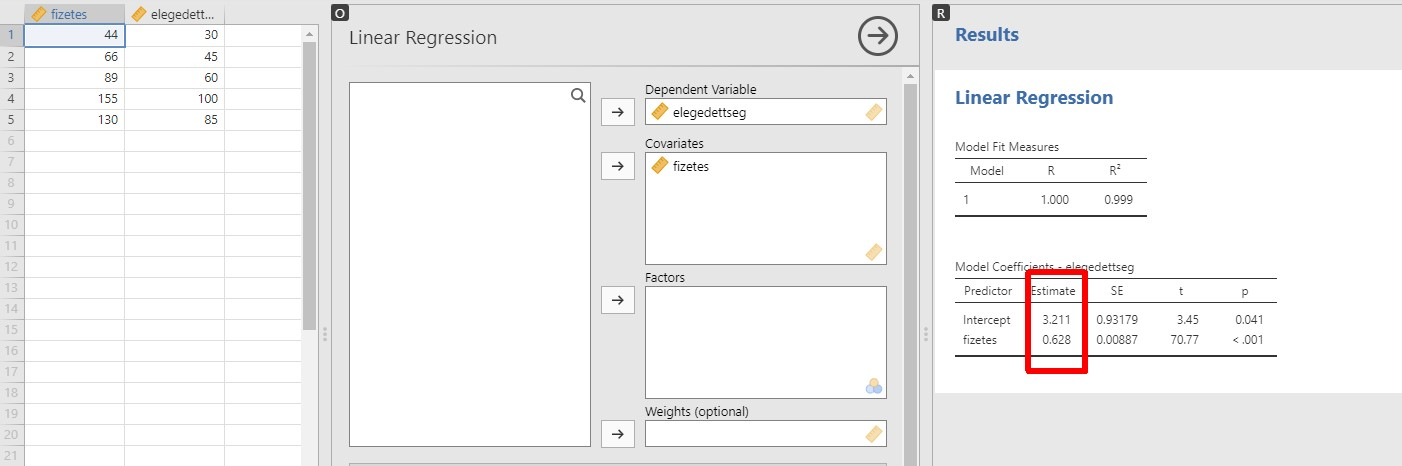
\includegraphics{./images/lin_reg_fizetes_elegedettseg_02_kep.jpg}

}

\caption{Fizetés és elégedettésg kapcsolata (N=5): együtthatók}

\end{figure}

A fenti elemzés alapján például a \(\hat{Y}=b_0+b_1 X\) konkrét formája:

\begin{Shaded}
\begin{Highlighting}[]
\NormalTok{becsült elégedettség = 3,211+ 0,628 * fizetés}
\end{Highlighting}
\end{Shaded}

\begin{itemize}
\tightlist
\item
  A \(b_0\) értelmezése: a zérus \(X\)-hez tartozó \(Y\) érték.
\item
  A \(b_1\) értelmezése: az \(X\) egy egységnyi növekedéséhez ilyen
  nagyságú \(Y\) változás tartozik.
\end{itemize}

Tudjuk, hogy az \(r_{XY}\) Pearson-féle korrelációs együttható, az \(X\)
és \(Y\) változók közötti kapcsolat erősségét és irányát mutatja meg. A
\(b_1\) és \(r_{XY}\) kapcsolatban áll:

\begin{itemize}
\tightlist
\item
  azonos az előjelük,
\item
  az \(X\) egy szórásnyi növekedéséhez tartozó \(Y\) változás megegyezik
  az \(Y\) szórásának \(r_{XY}\) szeresével (rövidebben, a populációbeli
  paraméterekkel megfogalmazva:
  \(\beta_1=\frac{\sigma_Y}{\sigma_X}\rho_{XY}\)
\end{itemize}

A determinációs együttható (\(R^2\)) a korrelációs együttható négyzete
\((R^2=r_{XY}^2)\), amely szimmetrikus mutató, megmutatja, hogy \(Y\)
varianciájának mekkora hányadát magyarázza \(X\) varianciája, vagy
fordítva, \(X\) varianciájának mekkora hányadát magyarázza \(Y\)
varianciája.

A fenti példában látható, hogy 99\%-ban lehet a függő változó
varianciáját magyarázni a független változóval (az arányt legtöbbször
százalékos formában adjuk meg).

\begin{Shaded}
\begin{Highlighting}[]
\FunctionTok{summary}\NormalTok{(lm\_1)}\SpecialCharTok{$}\NormalTok{r.squared}
\CommentTok{\#\textgreater{} [1] 0.9994014}
\end{Highlighting}
\end{Shaded}

\begin{figure}

{\centering 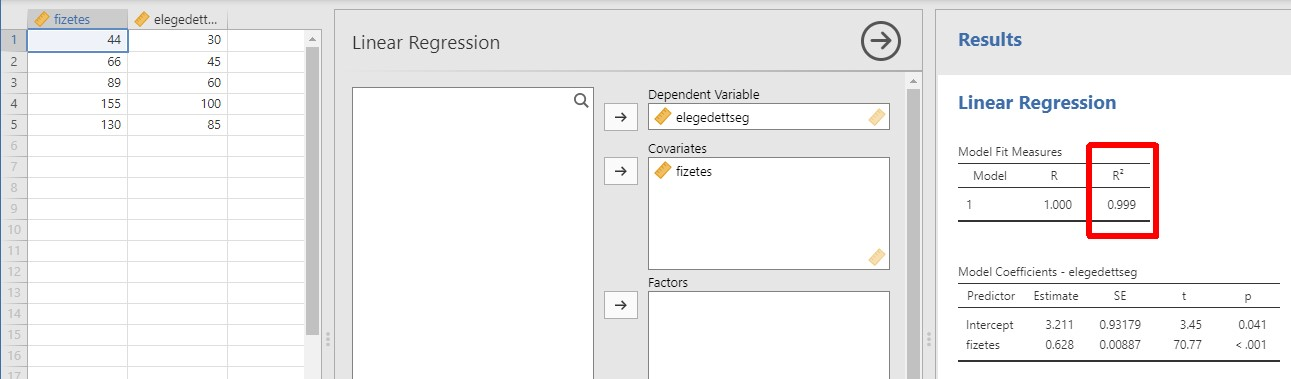
\includegraphics{./images/lin_reg_fizetes_elegedettseg_02_kep_02.jpg}

}

\caption{Fizetés és elégedettésg kapcsolata (N=5): determinációs
együttható}

\end{figure}

A \(\beta_0\) és \(\beta_1\) együtthatók értékét hipotézisvizsgálatokkal
vizsgálhatjuk:

\begin{itemize}
\tightlist
\item
  \(H_0\): \(\beta_0=0\), \(H_1: \beta_0 \neq 0\) Kérdés: origón átmenő
  a regresszió? (\(H_0\) megtartása esetén igen)
\item
  \(H_0\): \(\beta_1=0\), \(H_1: \beta_1 \neq 0\) Kérdés: \(Y\) függ
  \(X\)-től? (\(H_1\) elfogadása esetén igen)
\end{itemize}

A példában látható, hogy nem origón átmenő a regresszió, és az
elégedettség függ a fizetéstől.

\begin{Shaded}
\begin{Highlighting}[]
\FunctionTok{summary}\NormalTok{(lm\_1)}\SpecialCharTok{$}\NormalTok{coefficients}
\CommentTok{\#\textgreater{}              Estimate  Std. Error   t value     Pr(...}
\CommentTok{\#\textgreater{} (Intercept) 3.2108896 0.931790852  3.445934 4.10580...}
\CommentTok{\#\textgreater{} fizetes     0.6279867 0.008873152 70.773796 6.21643...}
\end{Highlighting}
\end{Shaded}

\begin{figure}

{\centering 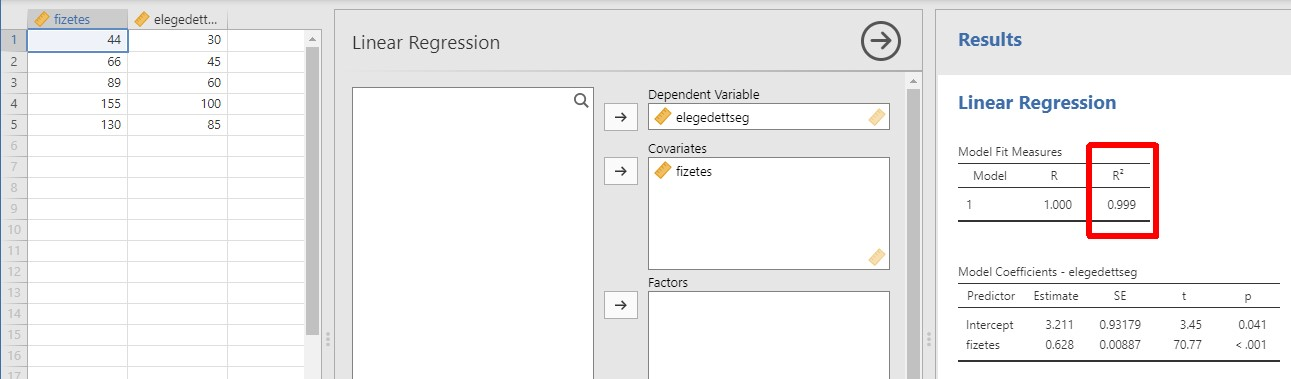
\includegraphics{./images/lin_reg_fizetes_elegedettseg_02_kep_02.jpg}

}

\caption{Fizetés és elégedettésg kapcsolata (N=5): hipotézisvizsgálat az
együtthatókra}

\end{figure}

\hypertarget{tuxf6bbszuxf6ruxf6s-lineuxe1ris-regressziuxf3}{%
\section{Többszörös lineáris
regresszió}\label{tuxf6bbszuxf6ruxf6s-lineuxe1ris-regressziuxf3}}

A többszörös lineáris regressziós modell:
\(Y=\beta_0+\beta_1 X_1+\beta_2 X_2+\dots + \beta_r X_r+\epsilon\).

Míg az egyszerű lineáris regresszió esetén a regressziós egyenes írta le
a két változó kapcsolatát, a többszörös lineáris regresszió esetén a
lineáris függvény egy \(r\) dimenziós sík az \(r+1\) dimenziós térben.

Az egyes \(\beta_i\) együtthatók becslése itt is a legkisebb négyzetek
elve alapján történik, így kapjuk a \(b_0, b_1, \dots, b_r\)
becsléseket.

A lineáris függvény birtokában tetszőleges \(X_1,X_2,\dots,X_r\)
értékekhez tudunk \(Y\) értéket előre jelezni, vagyis jósolni bizonyos
hibával: \(\hat{Y}=b_0+b_1 X_1+\dots+ b_r X_r\).

\begin{Shaded}
\begin{Highlighting}[]
\NormalTok{d }\OtherTok{\textless{}{-}}\NormalTok{ rio}\SpecialCharTok{::}\FunctionTok{import}\NormalTok{(}\AttributeTok{file =} \StringTok{"adat/lin\_reg\_fizetes\_eletkor\_elegedettseg\_01.xlsx"}\NormalTok{)}
\FunctionTok{str}\NormalTok{(d)}
\CommentTok{\#\textgreater{} \textquotesingle{}data.frame\textquotesingle{}:    5 obs. of  3 variables:}
\CommentTok{\#\textgreater{}  $ fizetes     : num  44 66 89 155 130}
\CommentTok{\#\textgreater{}  $ eletkor     : num  25 65 21 35 40}
\CommentTok{\#\textgreater{}  $ elegedettseg: num  37 36 61 92 76}
\NormalTok{d}
\CommentTok{\#\textgreater{}   fizetes eletkor elegedettseg}
\CommentTok{\#\textgreater{} 1      44      25           37}
\CommentTok{\#\textgreater{} 2      66      65           36}
\CommentTok{\#\textgreater{} 3      89      21           61}
\CommentTok{\#\textgreater{} 4     155      35           92}
\CommentTok{\#\textgreater{} 5     130      40           76}
\end{Highlighting}
\end{Shaded}

\begin{Shaded}
\begin{Highlighting}[]
\NormalTok{lm\_1 }\OtherTok{\textless{}{-}} \FunctionTok{lm}\NormalTok{(elegedettseg }\SpecialCharTok{\textasciitilde{}}\NormalTok{ fizetes }\SpecialCharTok{+}\NormalTok{ eletkor, }\AttributeTok{data =}\NormalTok{ d)}
\FunctionTok{summary}\NormalTok{(lm\_1)}
\CommentTok{\#\textgreater{} }
\CommentTok{\#\textgreater{} Call:}
\CommentTok{\#\textgreater{} lm(formula = elegedettseg \textasciitilde{} fizetes + eletkor, data...}
\CommentTok{\#\textgreater{} }
\CommentTok{\#\textgreater{} Residuals:}
\CommentTok{\#\textgreater{}        1        2        3        4        5 }
\CommentTok{\#\textgreater{}  0.28596  0.08556 {-}0.30015  0.71047 {-}0.78184 }
\CommentTok{\#\textgreater{} }
\CommentTok{\#\textgreater{} Coefficients:}
\CommentTok{\#\textgreater{}              Estimate Std. Error t value Pr(\textgreater{}|t|)    }
\CommentTok{\#\textgreater{} (Intercept) 21.508055   1.292166   16.64  0.00359 ** }
\CommentTok{\#\textgreater{} fizetes      0.519198   0.008847   58.69  0.00029 ***}
\CommentTok{\#\textgreater{} eletkor     {-}0.305549   0.023279  {-}13.12  0.00575 ** }
\CommentTok{\#\textgreater{} {-}{-}{-}}
\CommentTok{\#\textgreater{} Signif. codes:  }
\CommentTok{\#\textgreater{} 0 \textquotesingle{}***\textquotesingle{} 0.001 \textquotesingle{}**\textquotesingle{} 0.01 \textquotesingle{}*\textquotesingle{} 0.05 \textquotesingle{}.\textquotesingle{} 0.1 \textquotesingle{} \textquotesingle{} 1}
\CommentTok{\#\textgreater{} }
\CommentTok{\#\textgreater{} Residual standard error: 0.8047 on 2 degrees of fre...}
\CommentTok{\#\textgreater{} Multiple R{-}squared:  0.9995, Adjusted R{-}squared:  0...}
\CommentTok{\#\textgreater{} F{-}statistic:  1841 on 2 and 2 DF,  p{-}value: 0.000543}
\end{Highlighting}
\end{Shaded}

\begin{figure}

{\centering 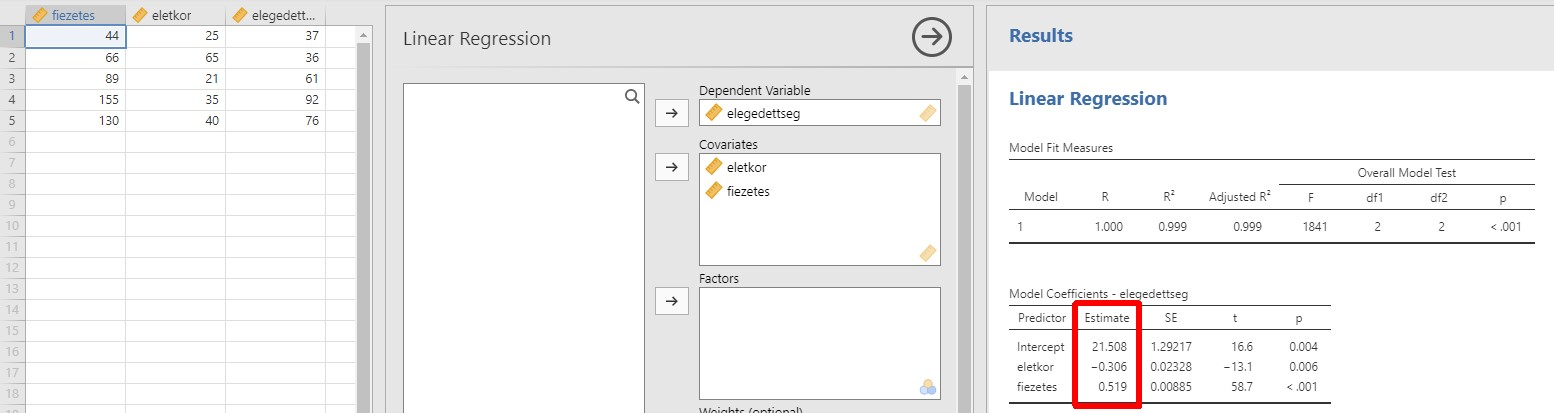
\includegraphics{./images/lin_reg_fizetes_eletkor_elegedettseg_01_kep_01.jpg}

}

\caption{Elégedettség kapcsolata a fizetéssel és az élekorral (N=5):
együtthatók}

\end{figure}

A fenti példában a lineáris regresszió futtatása után azt mondhatjuk:

\begin{Shaded}
\begin{Highlighting}[]
\NormalTok{becsült elégedettség = 21,05 {-}0,306*életkor + 0,519*fizetés}
\end{Highlighting}
\end{Shaded}

Más szavakkal a fizetés tekintetében a magasabb fizetés nagyobb mértékű
elégedettséggel jár, addig az életkor esetében az évek számának
növekedése a munkahellyel való elégedetlenséget vonja maga után.

\begin{itemize}
\tightlist
\item
  A \(b_0\) értelmezése: a csupa zérus \(X_1, X_2,\dots,X_r\)-ekhez
  tartozó \(Y\) érték.
\item
  A \(b_i\) \((i=1,\dots,r)\) értelmezése: az \(X_i\) hatása úgy, hogy a
  többi független változót is figyelembe vesszük.
\end{itemize}

A fenti többszörös lineáris regressziós együtthatók nem alkalmasak az
egyes magyarázó változóktól való függés erősségének mérésére, ugyanis a
nagyságuk függ a változó értékeinek nagyságától is. Ezért a standard
lineáris regressziós együtthatókat használjuk, amelyek már mértékegység
nélküli, egymással összehasonlítható arányszámok, így abszolút
értékeiket összevetve megtudhatjuk, milyen relatív fontossággal bírnak
az egyes független változók a függő változó magyarázásában.

\begin{Shaded}
\begin{Highlighting}[]
\NormalTok{lsr}\SpecialCharTok{::}\FunctionTok{standardCoefs}\NormalTok{(lm\_1)}
\CommentTok{\#\textgreater{}                  b       beta}
\CommentTok{\#\textgreater{} fizetes  0.5191980  0.9677518}
\CommentTok{\#\textgreater{} eletkor {-}0.3055489 {-}0.2164358}
\end{Highlighting}
\end{Shaded}

\begin{figure}

{\centering 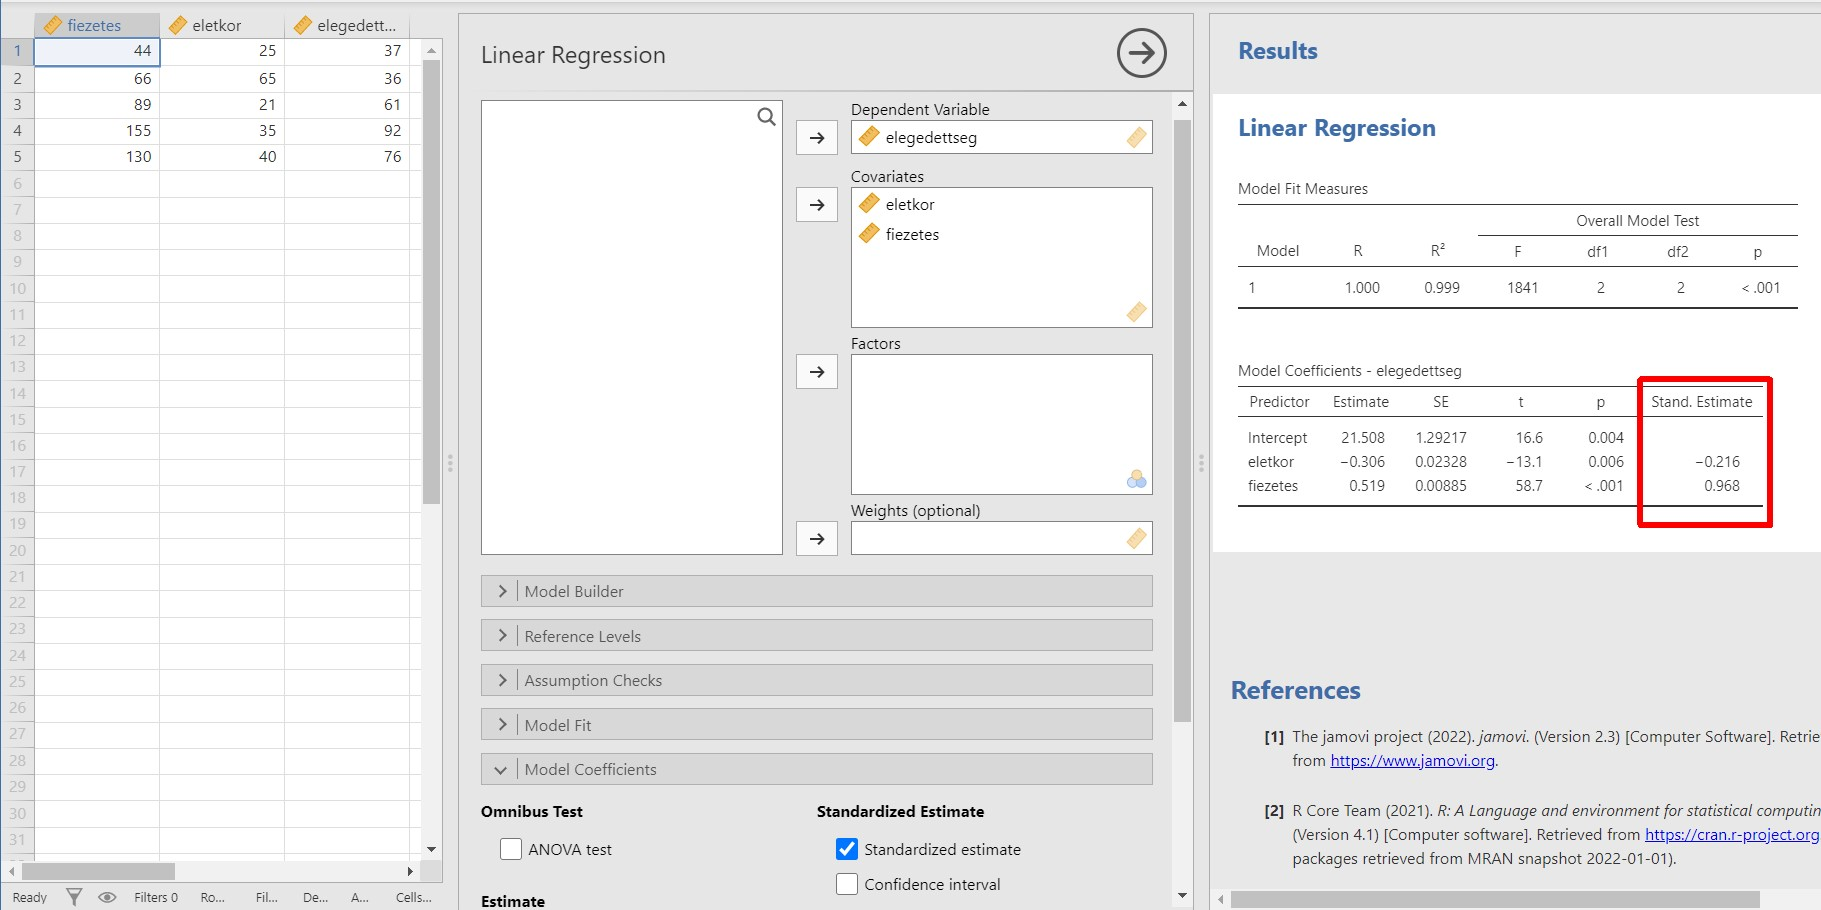
\includegraphics{./images/lin_reg_fizetes_eletkor_elegedettseg_01_kep_02.jpg}

}

\caption{Elégedettség kapcsolata a fizetéssel és az élekorral (N=5):
standardizált együtthatók}

\end{figure}

A fenti példában láthatjuk, hogy a fizetés erősebb kapcsolatban van az
elégedettséggel, hiszen a standardizált együtthatójának értéke abszolút
értékben nagyobb, mint az életkor standardizált együtthatójának abszolút
értéke.

Többszörös lineáris regresszió esetén több hipotézisvizsgálat végezhető:

\begin{itemize}
\tightlist
\item
  minden együtthatót külön tesztelhetünk t-próbákkal \((n-r-1)\)
  szabadsági fokkal

  \begin{itemize}
  \tightlist
  \item
    \(H_0:\beta_i=0\), \(H_1:\beta_i\neq0\), \(i=1,\dots,r\) Kérdés:
    \(Y\) függ \(X_i\)-től? (\(H_1\) elfogadása esetén igen)
  \end{itemize}
\item
  a teljes modellt tesztelhetjük F-próbával \((r,n-r-1)\) szabadsági
  fokkal

  \begin{itemize}
  \tightlist
  \item
    \(H_0: \text{minden } \beta_i=0\),
    \(H_1: \text{van olyan i, melyre } \beta_i\neq0\) Kérdés: a modell
    bír valamilyen bejósló erővel? (\(H_1\) elfogadása esetén igen)
  \end{itemize}
\end{itemize}

\begin{Shaded}
\begin{Highlighting}[]
\FunctionTok{summary}\NormalTok{(lm\_1)}\SpecialCharTok{$}\NormalTok{coefficients}
\CommentTok{\#\textgreater{}               Estimate Std. Error   t value     Pr(...}
\CommentTok{\#\textgreater{} (Intercept) 21.5080549 1.29216584  16.64496 0.00358...}
\CommentTok{\#\textgreater{} fizetes      0.5191980 0.00884672  58.68819 0.00029...}
\CommentTok{\#\textgreater{} eletkor     {-}0.3055489 0.02327903 {-}13.12550 0.00575...}
\FunctionTok{summary}\NormalTok{(lm\_1)}\SpecialCharTok{$}\NormalTok{fstatistic}
\CommentTok{\#\textgreater{}    value    numdf    dendf }
\CommentTok{\#\textgreater{} 1840.547    2.000    2.000}
\FunctionTok{pf}\NormalTok{(}\AttributeTok{q =} \FunctionTok{summary}\NormalTok{(lm\_1)}\SpecialCharTok{$}\NormalTok{fstatistic[}\DecValTok{1}\NormalTok{], }\AttributeTok{df1 =} \FunctionTok{summary}\NormalTok{(lm\_1)}\SpecialCharTok{$}\NormalTok{fstatistic[}\DecValTok{2}\NormalTok{],}
    \AttributeTok{df2 =} \FunctionTok{summary}\NormalTok{(lm\_1)}\SpecialCharTok{$}\NormalTok{fstatistic[}\DecValTok{3}\NormalTok{], }\AttributeTok{lower.tail =}\NormalTok{ F)}
\CommentTok{\#\textgreater{}        value }
\CommentTok{\#\textgreater{} 0.0005430217}
\end{Highlighting}
\end{Shaded}

\begin{figure}

{\centering 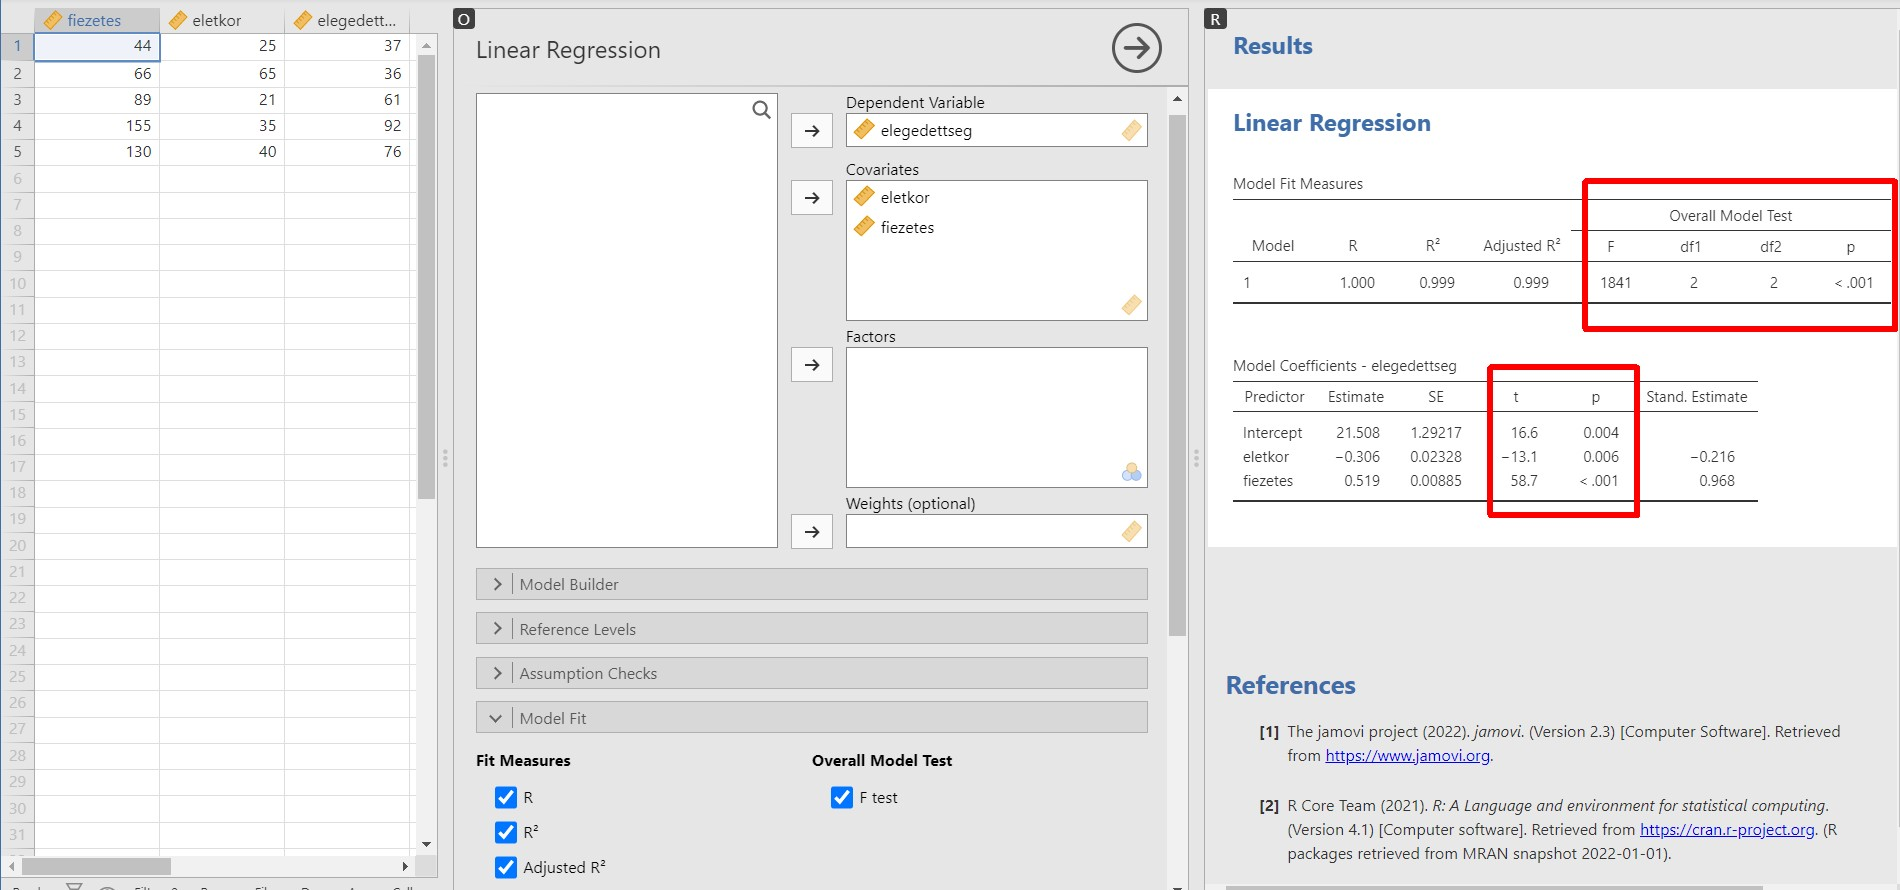
\includegraphics{./images/lin_reg_fizetes_eletkor_elegedettseg_01_kep_03.jpg}

}

\caption{Elégedettség kapcsolata a fizetéssel és az élekorral (N=5):
hipotézisvizsgálatok}

\end{figure}

A lenti példában látható, hogy mindkét magyarázó változótól függ az
elégedettség (életkor p-értéke: 0,006, a fizetés p-értéke p \textless{}
0,001), és a teljes modell bír magyarázó erővel (p-érték: p \textless{}
0,001).

A függő változó és a független változók közötti korreláció erősségének
leírására több mennyiséget használhatunk

\begin{itemize}
\item
  többszörös korrelációs együttható: \(R\), amely a függő változó és a
  becsült értékek közötti korrelációs együttható értékével egyezik meg,
  azaz \(R(Y,X_1,X_2,…,X_r )=R(Y,\hat{Y})\). Valójában a lineáris
  regresszió ennek a korrelációs együtthatónak az értékét maximalizálja,
  mikor az \(\hat{Y}\)-t \(X\)-ek speciális lineáris kombinációjaként
  előállítja.
\item
  többszörös determinációs együttható: \(R^2\), amely a többszörös
  korrelációs együttható négyzete, és megmutatja, hogy a magyarázó
  változók a függő változó ingadozásának hányad részét magyarázzák.
\item
  korrigált determinációs együttható: \(R_{adj}^2\), amely kiküszöböli
  az \(R^2\) azon tulajdonságát, hogy a magyarázó változók számának
  növekedésével, függetlenül azok hatásától, nő az értéke. Így alkalmas
  több modell esetén a magyarázó erők összehasonlítására, akkor is, ha
  azok eltérő számú független változót használnak.
\end{itemize}

\begin{Shaded}
\begin{Highlighting}[]
\FunctionTok{summary}\NormalTok{(lm\_1)}\SpecialCharTok{$}\NormalTok{r.squared}
\CommentTok{\#\textgreater{} [1] 0.999457}
\FunctionTok{summary}\NormalTok{(lm\_1)}\SpecialCharTok{$}\NormalTok{adj.r.squared}
\CommentTok{\#\textgreater{} [1] 0.998914}
\end{Highlighting}
\end{Shaded}

\begin{figure}

{\centering 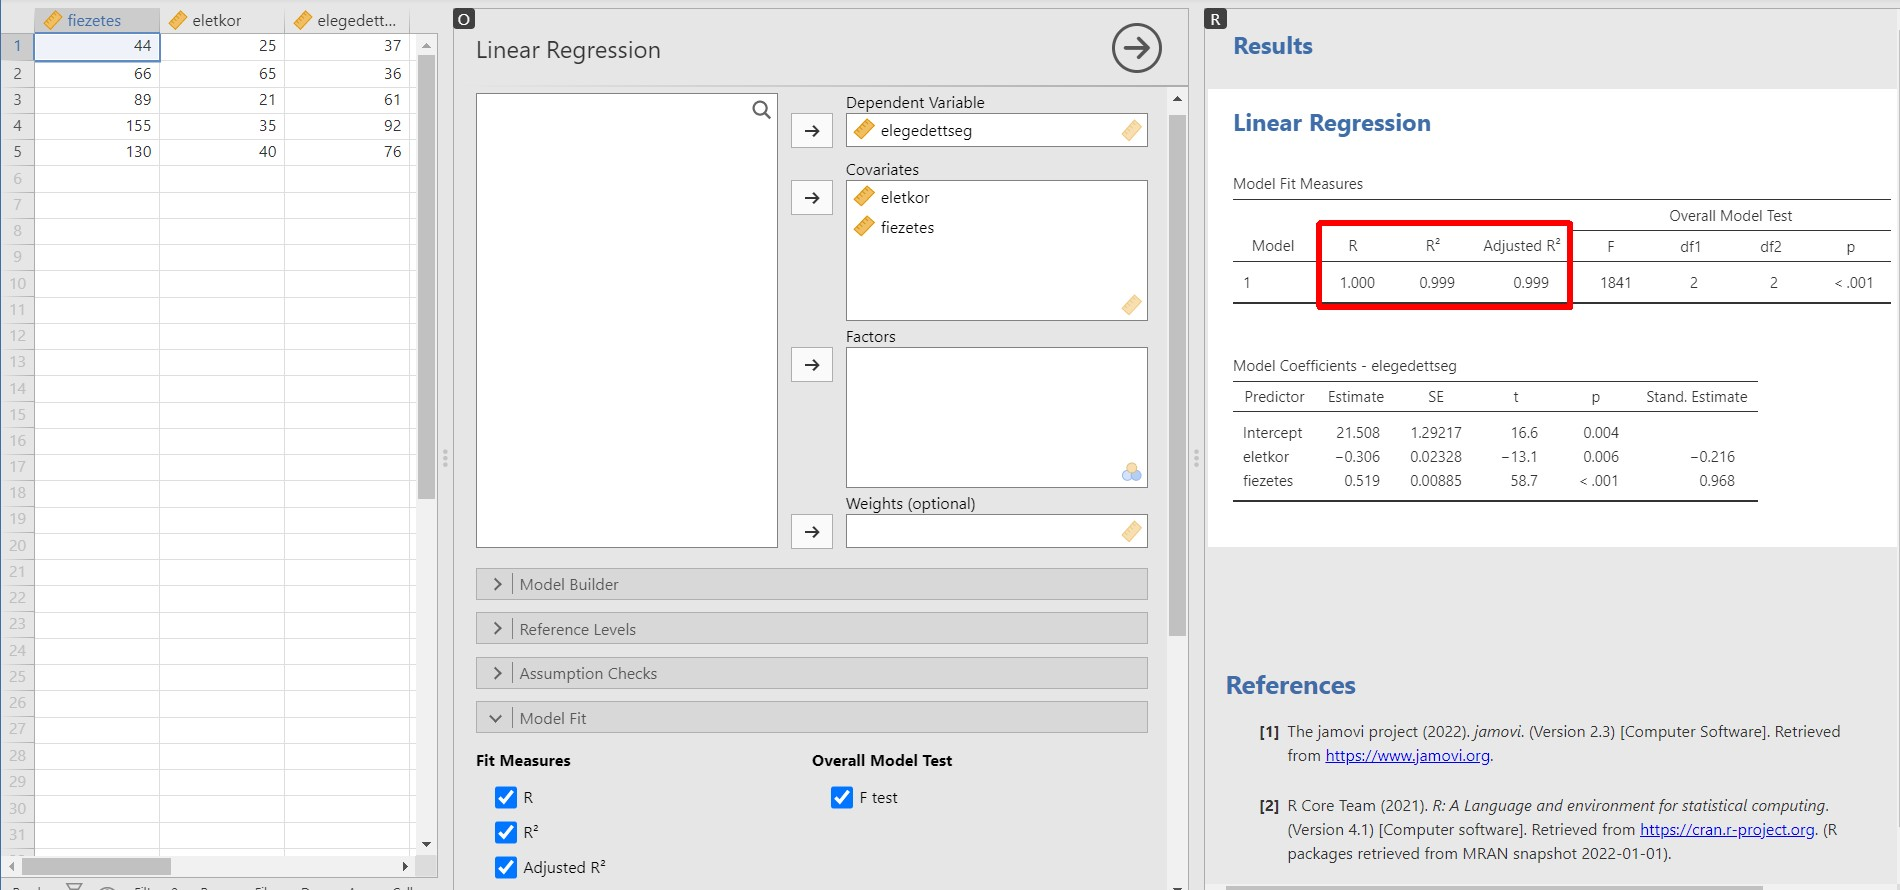
\includegraphics{./images/lin_reg_fizetes_eletkor_elegedettseg_01_kep_04.jpg}

}

\caption{Elégedettség kapcsolata a fizetéssel és az élekorral (N=5):
magyarázó erő}

\end{figure}

A fenti példában látható mindhárom fenti mutató. Az \(R_{adj}^2\)
leolvasásával láthatjuk, hogy a két független változó, az életkor és a
fizetés a függő változó 99\%-át magyarázza.

\hypertarget{parciuxe1lis-korreluxe1ciuxf3s-egyuxfctthatuxf3}{%
\section{Parciális korrelációs
együttható}\label{parciuxe1lis-korreluxe1ciuxf3s-egyuxfctthatuxf3}}

Parciális korrelációs együttható: két változó (\(S_1,S_2\)) közötti
korreláció mértéke, miután változók egy halmazának
\((T_1,T_2,\dots,T_g)\) a két változó korrelációjára vonatkozó hatását
többszörös lineáris regresszióval kiküszöböljük:

\begin{itemize}
\tightlist
\item
  \(R( S_1,S_2 |T_1,T_2,\dots,T_g )= R(S_1- \hat{S_1},S_2- \hat{S_2})\),
  ahol \(\hat{S_1}\) és \(\hat{S_2}\) az \(S_1\) és \(S_2\) változó
  többszörös lineáris regresszióból származó becslése a
  \(T_1,T_2,\dots,T_g\) magyarázó változók esetén.
\end{itemize}

\begin{Shaded}
\begin{Highlighting}[]
\NormalTok{d }\OtherTok{\textless{}{-}}\NormalTok{ rio}\SpecialCharTok{::}\FunctionTok{import}\NormalTok{(}\AttributeTok{file =} \StringTok{"adat/lin\_reg\_intelligencia\_testmagassag\_eletkor\_01.xlsx"}\NormalTok{)}
\FunctionTok{str}\NormalTok{(d)}
\CommentTok{\#\textgreater{} \textquotesingle{}data.frame\textquotesingle{}:    5 obs. of  3 variables:}
\CommentTok{\#\textgreater{}  $ intelligencia: num  81 86 91 101 111}
\CommentTok{\#\textgreater{}  $ testmagassag : num  138 145 156 163 167}
\CommentTok{\#\textgreater{}  $ eletkor      : num  9 12 14 18 22}
\NormalTok{d}
\CommentTok{\#\textgreater{}   intelligencia testmagassag eletkor}
\CommentTok{\#\textgreater{} 1            81          138       9}
\CommentTok{\#\textgreater{} 2            86          145      12}
\CommentTok{\#\textgreater{} 3            91          156      14}
\CommentTok{\#\textgreater{} 4           101          163      18}
\CommentTok{\#\textgreater{} 5           111          167      22}
\end{Highlighting}
\end{Shaded}

\begin{Shaded}
\begin{Highlighting}[]
\FunctionTok{cor.test}\NormalTok{(d}\SpecialCharTok{$}\NormalTok{intelligencia, d}\SpecialCharTok{$}\NormalTok{testmagassag)}
\CommentTok{\#\textgreater{} }
\CommentTok{\#\textgreater{}  Pearson\textquotesingle{}s product{-}moment correlation}
\CommentTok{\#\textgreater{} }
\CommentTok{\#\textgreater{} data:  d$intelligencia and d$testmagassag}
\CommentTok{\#\textgreater{} t = 5.4629, df = 3, p{-}value = 0.01205}
\CommentTok{\#\textgreater{} alternative hypothesis: true correlation is not equ...}
\CommentTok{\#\textgreater{} 95 percent confidence interval:}
\CommentTok{\#\textgreater{}  0.4463631 0.9970093}
\CommentTok{\#\textgreater{} sample estimates:}
\CommentTok{\#\textgreater{}      cor }
\CommentTok{\#\textgreater{} 0.953235}
\NormalTok{RcmdrMisc}\SpecialCharTok{::}\FunctionTok{partial.cor}\NormalTok{(d, }\AttributeTok{tests =}\NormalTok{ T)}
\CommentTok{\#\textgreater{} }
\CommentTok{\#\textgreater{}  Partial correlations:}
\CommentTok{\#\textgreater{}               intelligencia testmagassag eletkor}
\CommentTok{\#\textgreater{} intelligencia       0.00000     {-}0.46317 0.97875}
\CommentTok{\#\textgreater{} testmagassag       {-}0.46317      0.00000 0.62856}
\CommentTok{\#\textgreater{} eletkor             0.97875      0.62856 0.00000}
\CommentTok{\#\textgreater{} }
\CommentTok{\#\textgreater{}  Number of observations: 5 }
\CommentTok{\#\textgreater{} }
\CommentTok{\#\textgreater{}  Pairwise two{-}sided p{-}values:}
\CommentTok{\#\textgreater{}               intelligencia testmagassag eletkor}
\CommentTok{\#\textgreater{} intelligencia               0.5368       0.0213 }
\CommentTok{\#\textgreater{} testmagassag  0.5368                     0.3714 }
\CommentTok{\#\textgreater{} eletkor       0.0213        0.3714              }
\CommentTok{\#\textgreater{} }
\CommentTok{\#\textgreater{}  Adjusted p{-}values (Holm\textquotesingle{}s method)}
\CommentTok{\#\textgreater{}               intelligencia testmagassag eletkor}
\CommentTok{\#\textgreater{} intelligencia               0.7429       0.0638 }
\CommentTok{\#\textgreater{} testmagassag  0.7429                     0.7429 }
\CommentTok{\#\textgreater{} eletkor       0.0638        0.7429}
\end{Highlighting}
\end{Shaded}

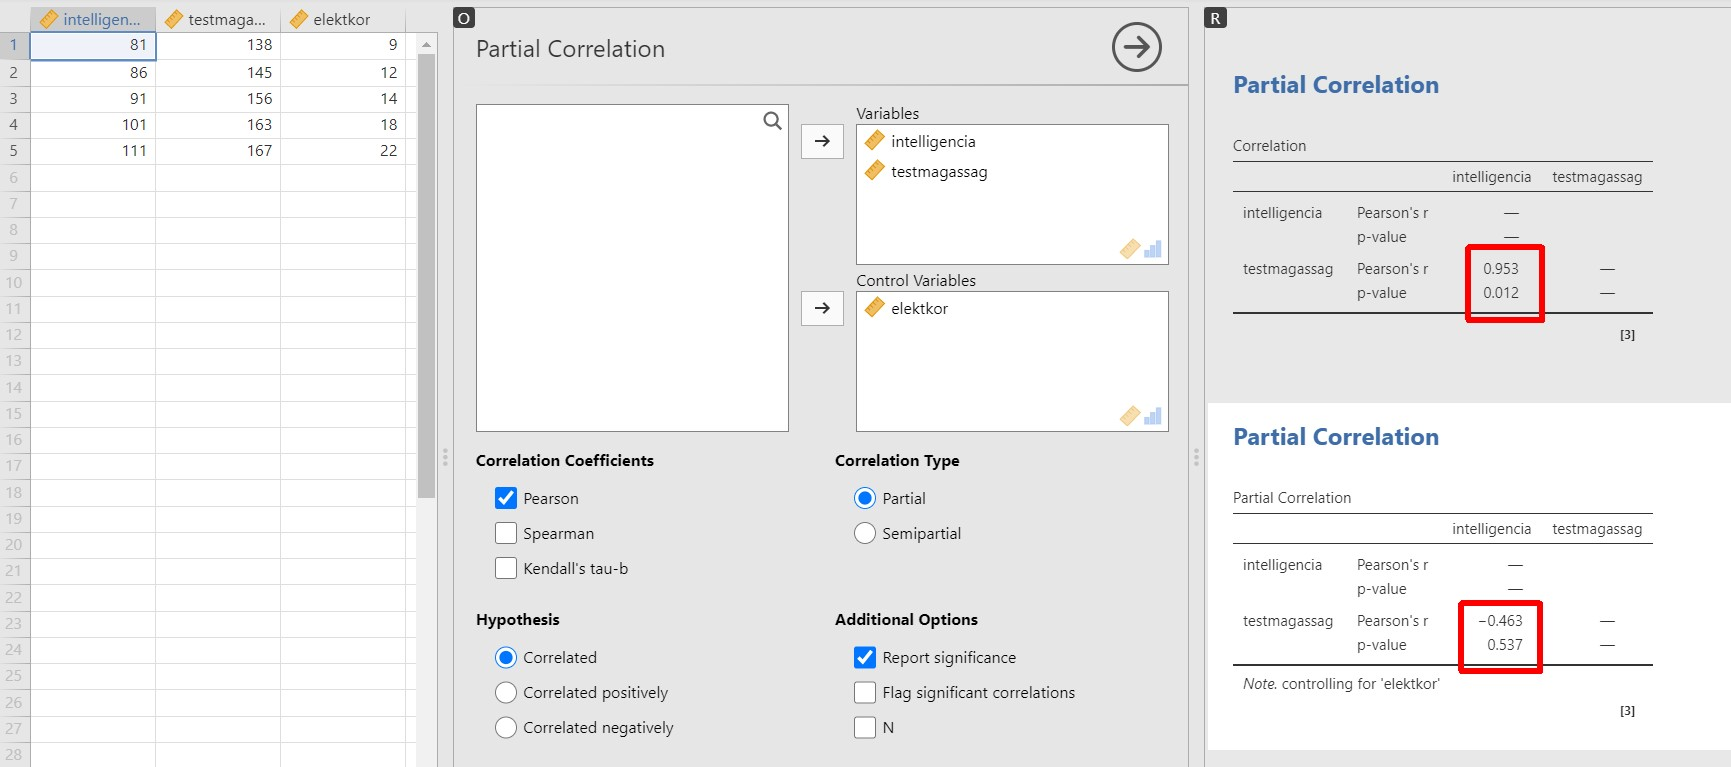
\includegraphics{./images/lin_reg_intelligencia_testmagassag_eletkor_01_kep_01.jpg}
A fenti példában látható, hogy míg szignifikáns erős pozitív kapcsolat
van az intelligencia és a magasság között (korrelációs együttható:
\(r=0,95; p=0,012\)), ez a kapcsolat eltűnik, ha figyelembe vesszük az
életkor változót is (parciális korreláció: \(r_{par}=-0,46; p=0,537\)).
Vagyis sikerült az intelligencia és a testmagasság közötti kapcsolat
erősségét megállapítani, miközben az életkor hatását erre a kapcsolatra
kiküszöböltük.

A többszörös lineáris regressziós modell
\((Y=\beta_0+\beta_1 X_1+\beta_2 X_2+\dots+\beta_r X_r+\epsilon)\)
becsült paraméterei \((b_1,b_2,…,b_r)\) nagyban hasonlítanak a parciális
korrelációs együtthatókra, mivel minden \(b_i\) az \(Y\) és \(X_i\)
közötti kapcsolat erősségét írja le, miközben a többi magyarázó változó
(\(X_1,X_2,\dots,X_r\), összesen \((r-1)\) db, \(X_i\) nincs köztük)
hatását kiküszöböljük a két változó korrelációjából.

A parciális korrelációs együtthatók és a többszörös lineáris regresszió
együtthatói között annyira közvetlen a kapcsolat, hogy azonos p-érték
tartozik hozzájuk, mint a lenti példában ez látható is lesz.

A lenti példában két modell szerepel, először az intelligencia és a
testmagasság függvényszerű kapcsolatát vizsgáljuk és azt a meglepő
dolgot tapasztaljuk, hogy minél magasabb valaki, annál intelligensebb
\((p=0,012)\), majd ha bevonjuk az életkor változót, akkor azt
tapasztalhatjuk, hogy eltűnik az intelligencia és a testmagasság közötti
kapcsolat \((p=0,537)\).

\begin{Shaded}
\begin{Highlighting}[]
\NormalTok{lm\_1 }\OtherTok{\textless{}{-}} \FunctionTok{lm}\NormalTok{(intelligencia }\SpecialCharTok{\textasciitilde{}}\NormalTok{ testmagassag, }\AttributeTok{data =}\NormalTok{ d)}
\FunctionTok{summary}\NormalTok{(lm\_1)}
\CommentTok{\#\textgreater{} }
\CommentTok{\#\textgreater{} Call:}
\CommentTok{\#\textgreater{} lm(formula = intelligencia \textasciitilde{} testmagassag, data = d)}
\CommentTok{\#\textgreater{} }
\CommentTok{\#\textgreater{} Residuals:}
\CommentTok{\#\textgreater{}       1       2       3       4       5 }
\CommentTok{\#\textgreater{}  1.9228  0.3114 {-}5.0779 {-}1.6892  4.5328 }
\CommentTok{\#\textgreater{} }
\CommentTok{\#\textgreater{} Coefficients:}
\CommentTok{\#\textgreater{}              Estimate Std. Error t value Pr(\textgreater{}|t|)  }
\CommentTok{\#\textgreater{} (Intercept)  {-}51.2613    26.6569  {-}1.923   0.1502  }
\CommentTok{\#\textgreater{} testmagassag   0.9445     0.1729   5.463   0.0121 *}
\CommentTok{\#\textgreater{} {-}{-}{-}}
\CommentTok{\#\textgreater{} Signif. codes:  }
\CommentTok{\#\textgreater{} 0 \textquotesingle{}***\textquotesingle{} 0.001 \textquotesingle{}**\textquotesingle{} 0.01 \textquotesingle{}*\textquotesingle{} 0.05 \textquotesingle{}.\textquotesingle{} 0.1 \textquotesingle{} \textquotesingle{} 1}
\CommentTok{\#\textgreater{} }
\CommentTok{\#\textgreater{} Residual standard error: 4.202 on 3 degrees of freedom}
\CommentTok{\#\textgreater{} Multiple R{-}squared:  0.9087, Adjusted R{-}squared:  0...}
\CommentTok{\#\textgreater{} F{-}statistic: 29.84 on 1 and 3 DF,  p{-}value: 0.01205}
\NormalTok{lm\_2 }\OtherTok{\textless{}{-}} \FunctionTok{lm}\NormalTok{(intelligencia }\SpecialCharTok{\textasciitilde{}}\NormalTok{ testmagassag }\SpecialCharTok{+}\NormalTok{ eletkor, }\AttributeTok{data =}\NormalTok{ d)}
\FunctionTok{summary}\NormalTok{(lm\_2)}
\CommentTok{\#\textgreater{} }
\CommentTok{\#\textgreater{} Call:}
\CommentTok{\#\textgreater{} lm(formula = intelligencia \textasciitilde{} testmagassag + eletkor...}
\CommentTok{\#\textgreater{} }
\CommentTok{\#\textgreater{} Residuals:}
\CommentTok{\#\textgreater{}        1        2        3        4        5 }
\CommentTok{\#\textgreater{}  0.89121 {-}1.16330 {-}0.09995  0.21170  0.16034 }
\CommentTok{\#\textgreater{} }
\CommentTok{\#\textgreater{} Coefficients:}
\CommentTok{\#\textgreater{}              Estimate Std. Error t value Pr(\textgreater{}|t|)  }
\CommentTok{\#\textgreater{} (Intercept)   73.1026    19.6042   3.729   0.0650 .}
\CommentTok{\#\textgreater{} testmagassag  {-}0.1210     0.1637  {-}0.739   0.5368  }
\CommentTok{\#\textgreater{} eletkor        2.6338     0.3902   6.750   0.0213 *}
\CommentTok{\#\textgreater{} {-}{-}{-}}
\CommentTok{\#\textgreater{} Signif. codes:  }
\CommentTok{\#\textgreater{} 0 \textquotesingle{}***\textquotesingle{} 0.001 \textquotesingle{}**\textquotesingle{} 0.01 \textquotesingle{}*\textquotesingle{} 0.05 \textquotesingle{}.\textquotesingle{} 0.1 \textquotesingle{} \textquotesingle{} 1}
\CommentTok{\#\textgreater{} }
\CommentTok{\#\textgreater{} Residual standard error: 1.055 on 2 degrees of freedom}
\CommentTok{\#\textgreater{} Multiple R{-}squared:  0.9962, Adjusted R{-}squared:  0...}
\CommentTok{\#\textgreater{} F{-}statistic: 259.3 on 2 and 2 DF,  p{-}value: 0.003841}
\end{Highlighting}
\end{Shaded}

\begin{figure}

{\centering 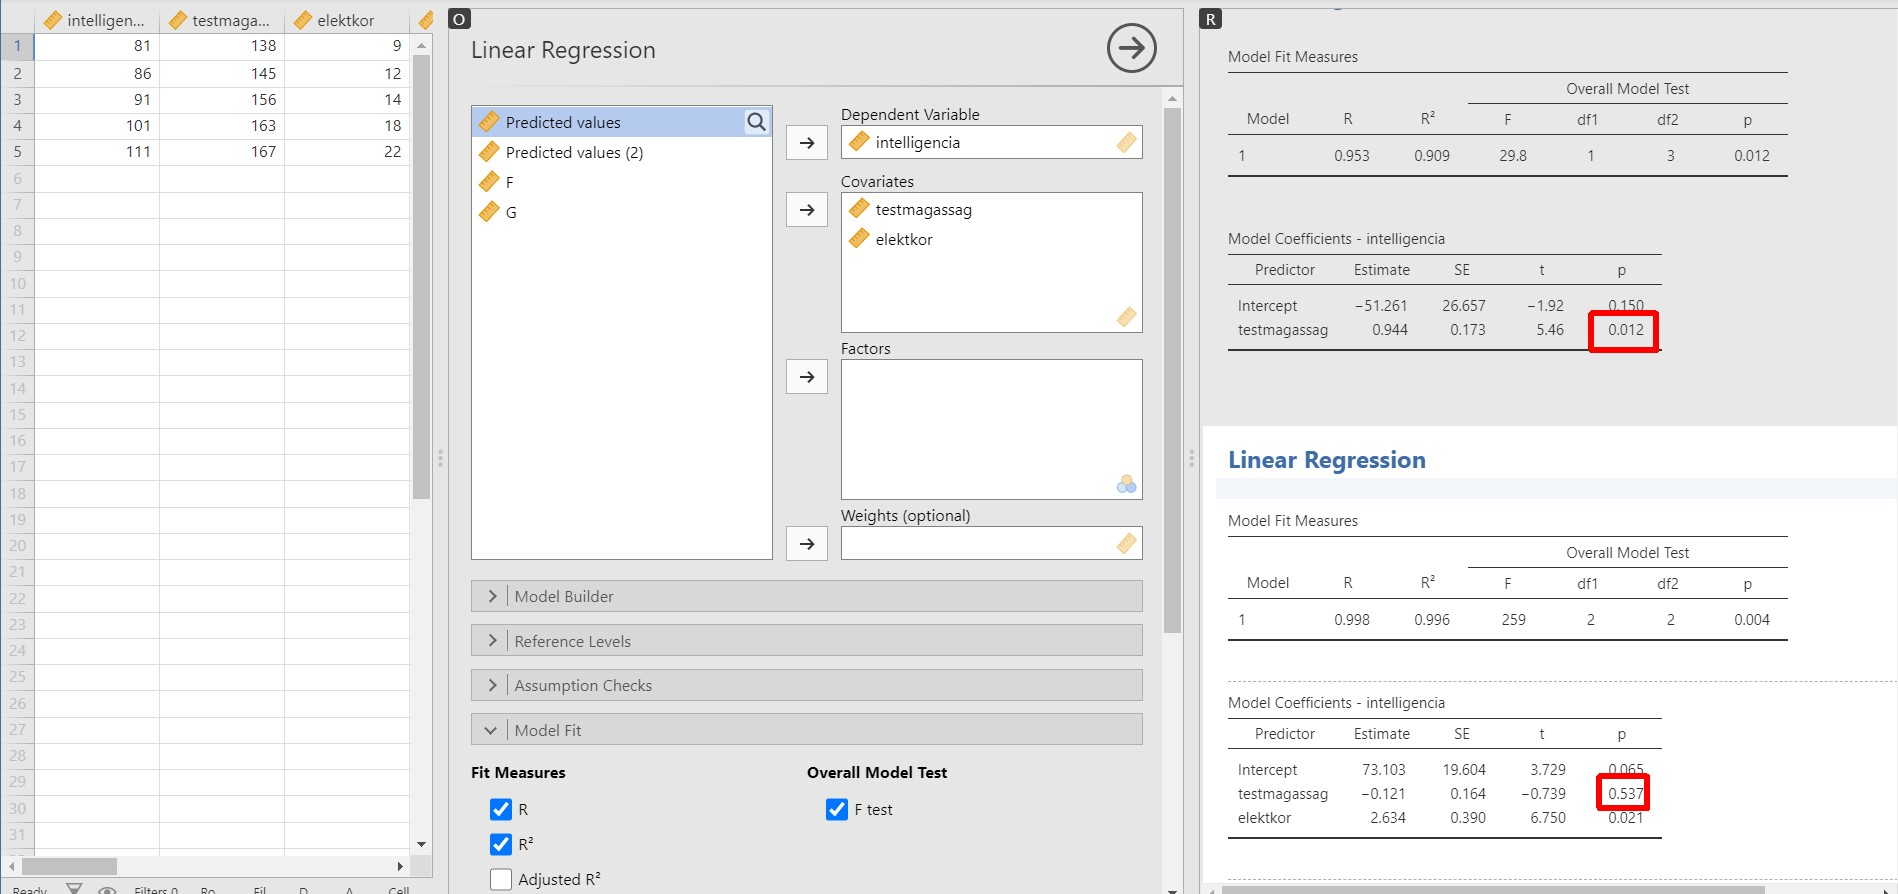
\includegraphics{./images/lin_reg_intelligencia_testmagassag_eletkor_01_kep_02.jpg}

}

\caption{Az intelligencia és a testmagasság kapcsolata (N=5): két
modell, életkor nélkül és életkorral}

\end{figure}

\hypertarget{a-tuxf6bbszuxf6ruxf6s-lineuxe1ris-regressziuxf3-esetei}{%
\section{A többszörös lineáris regresszió
esetei}\label{a-tuxf6bbszuxf6ruxf6s-lineuxe1ris-regressziuxf3-esetei}}

\hypertarget{egyetlen-dichotuxf3m-magyaruxe1zuxf3-vuxe1ltozuxf3}{%
\subsection{Egyetlen dichotóm magyarázó
változó}\label{egyetlen-dichotuxf3m-magyaruxe1zuxf3-vuxe1ltozuxf3}}

A magyarázó változóink eddig kvantitatívak voltak, de kategorikus
változók is lehetnek. Ha a kategorikus változónk csupán 2 értékű, akkor
a becsült (\(b_0\), \(b_1\)) együtthatók értelmezése módosul. A
tengelymetszet (\(b_0\)) a kategorikus változó referencia szintjén a
függő változó átlagát tartalmazza, míg a (\(b_1\)) a kategorikus változó
másik szintjén számolt átlag eltérését a \(b_0\)-hoz képest.

\begin{Shaded}
\begin{Highlighting}[]
\NormalTok{d }\OtherTok{\textless{}{-}}\NormalTok{ rio}\SpecialCharTok{::}\FunctionTok{import}\NormalTok{(}\AttributeTok{file =} \StringTok{"adat/lin\_reg\_magassag\_hajhossz\_nem\_01.xlsx"}\NormalTok{)}
\NormalTok{d}\SpecialCharTok{$}\NormalTok{nem }\OtherTok{\textless{}{-}} \FunctionTok{factor}\NormalTok{(d}\SpecialCharTok{$}\NormalTok{nem, }\AttributeTok{levels =} \FunctionTok{c}\NormalTok{(}\StringTok{"nő"}\NormalTok{, }\StringTok{"férfi"}\NormalTok{))}
\FunctionTok{str}\NormalTok{(d)}
\CommentTok{\#\textgreater{} \textquotesingle{}data.frame\textquotesingle{}:    6 obs. of  3 variables:}
\CommentTok{\#\textgreater{}  $ magassag: num  158 159 162 170 182 179}
\CommentTok{\#\textgreater{}  $ hajhossz: num  28 25 20 1 1.5 3}
\CommentTok{\#\textgreater{}  $ nem     : Factor w/ 2 levels "nő","férfi": 1 1 1...}
\NormalTok{d}
\CommentTok{\#\textgreater{}   magassag hajhossz   nem}
\CommentTok{\#\textgreater{} 1      158     28.0    nő}
\CommentTok{\#\textgreater{} 2      159     25.0    nő}
\CommentTok{\#\textgreater{} 3      162     20.0    nő}
\CommentTok{\#\textgreater{} 4      170      1.0 férfi}
\CommentTok{\#\textgreater{} 5      182      1.5 férfi}
\CommentTok{\#\textgreater{} 6      179      3.0 férfi}
\end{Highlighting}
\end{Shaded}

\begin{Shaded}
\begin{Highlighting}[]
\NormalTok{lm\_1 }\OtherTok{\textless{}{-}} \FunctionTok{lm}\NormalTok{(magassag }\SpecialCharTok{\textasciitilde{}}\NormalTok{ nem, }\AttributeTok{data =}\NormalTok{ d)}
\FunctionTok{summary}\NormalTok{(lm\_1)}
\CommentTok{\#\textgreater{} }
\CommentTok{\#\textgreater{} Call:}
\CommentTok{\#\textgreater{} lm(formula = magassag \textasciitilde{} nem, data = d)}
\CommentTok{\#\textgreater{} }
\CommentTok{\#\textgreater{} Residuals:}
\CommentTok{\#\textgreater{}       1       2       3       4       5       6 }
\CommentTok{\#\textgreater{} {-}1.6667 {-}0.6667  2.3333 {-}7.0000  5.0000  2.0000 }
\CommentTok{\#\textgreater{} }
\CommentTok{\#\textgreater{} Coefficients:}
\CommentTok{\#\textgreater{}             Estimate Std. Error t value Pr(\textgreater{}|t|)    }
\CommentTok{\#\textgreater{} (Intercept)  159.667      2.687  59.413 4.81e{-}07 ***}
\CommentTok{\#\textgreater{} nemférfi      17.333      3.801   4.561   0.0103 *  }
\CommentTok{\#\textgreater{} {-}{-}{-}}
\CommentTok{\#\textgreater{} Signif. codes:  }
\CommentTok{\#\textgreater{} 0 \textquotesingle{}***\textquotesingle{} 0.001 \textquotesingle{}**\textquotesingle{} 0.01 \textquotesingle{}*\textquotesingle{} 0.05 \textquotesingle{}.\textquotesingle{} 0.1 \textquotesingle{} \textquotesingle{} 1}
\CommentTok{\#\textgreater{} }
\CommentTok{\#\textgreater{} Residual standard error: 4.655 on 4 degrees of freedom}
\CommentTok{\#\textgreater{} Multiple R{-}squared:  0.8387, Adjusted R{-}squared:  0...}
\CommentTok{\#\textgreater{} F{-}statistic:  20.8 on 1 and 4 DF,  p{-}value: 0.01033}
\end{Highlighting}
\end{Shaded}

\begin{figure}

{\centering 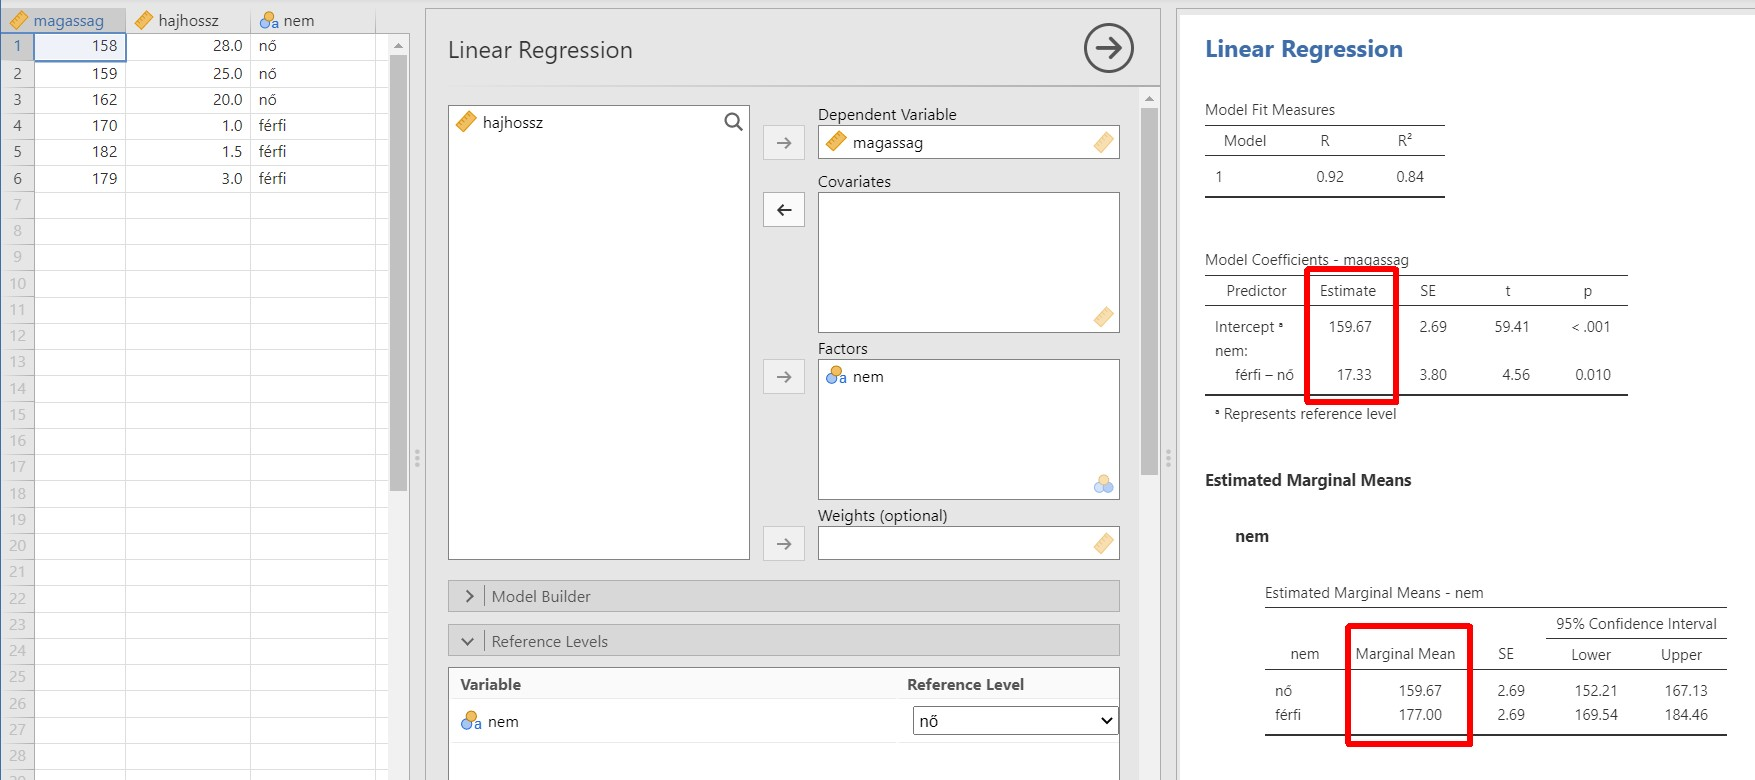
\includegraphics{./images/lin_reg_magassag_hajhossz_nem_01_kep_01.jpg}

}

\caption{A magasság és a nem kapcsolata}

\end{figure}

A fenti példa a nem hatását vizsgálja testmagasságra. A p-érték alapján
ez a hatás szignifikáns, tehát a függés fennáll, a paraméterek pedig a
nők átlagáról \((b_0=159,67)\) és a férfiak és nők átlagának eltéréséről
tájékoztatnak \((b_1=17,33)\).

\hypertarget{modellvuxe1lasztuxe1s}{%
\section{Modellválasztás}\label{modellvuxe1lasztuxe1s}}

Előfordulhat, hogy egy jelenség vizsgálatakor több lineáris regressziós
modellt is meg tudunk fogalmazni, nem csak egyetlen modell létezik. Ez a
probléma leggyakrabban úgy jelenik meg, hogy rengeteg független
változónk van, és nem tudjuk eldönteni, hogy elég egy kisebb modell,
néhány változóval, vagy vegyük inkább a nagyobb modellt több változóval.

A megfelelő modell megtaláláshoz a modelleket összehasonlíthatjuk
F-próba segítségével, szignifikáns eredmény esetén a két modell
magyarázó ereje eltér egymástól. Ilyenkor a célunk a legszűkebb
(legkevesebb magyarázó változót tartalmazó), de a legbővebbtől
szignifikánsan nem különböző modell megtalálása.

A korrigált determinációs együttható \((R_{adj}^2)\) is alkalmas mód a
modellek összehasonlítására: az 1-hez legközelebbi értékkel bíró modell
rendelkezik a legnagyobb magyarázó erővel. Léteznek már kritériumok is:

\begin{itemize}
\tightlist
\item
  AIC (Akaike-kritérium): minél kisebb az AIC értéke, annál nagyobb a
  modell magyarázó ereje.
\item
  BIC (Bayes-kritérium): minél kisebb a BIC értéke, annál nagyobb a
  modell magyarázó ereje.
\item
  RMSE (négyzetes középérték, Root Mean Square Error) az a mennyiség,
  amennyivel a vizsgált értékek eltérnek az előre megbecsült értékektől.
  Minél kisebb ez az érték, annál jobban becsül a modell.
\end{itemize}

\begin{Shaded}
\begin{Highlighting}[]
\NormalTok{d }\OtherTok{\textless{}{-}}\NormalTok{ rio}\SpecialCharTok{::}\FunctionTok{import}\NormalTok{(}\AttributeTok{file =} \StringTok{"adat/lin\_reg\_fizetes\_eletkor\_elegedettseg\_01.xlsx"}\NormalTok{)}
\FunctionTok{str}\NormalTok{(d)}
\CommentTok{\#\textgreater{} \textquotesingle{}data.frame\textquotesingle{}:    5 obs. of  3 variables:}
\CommentTok{\#\textgreater{}  $ fizetes     : num  44 66 89 155 130}
\CommentTok{\#\textgreater{}  $ eletkor     : num  25 65 21 35 40}
\CommentTok{\#\textgreater{}  $ elegedettseg: num  37 36 61 92 76}
\NormalTok{d}
\CommentTok{\#\textgreater{}   fizetes eletkor elegedettseg}
\CommentTok{\#\textgreater{} 1      44      25           37}
\CommentTok{\#\textgreater{} 2      66      65           36}
\CommentTok{\#\textgreater{} 3      89      21           61}
\CommentTok{\#\textgreater{} 4     155      35           92}
\CommentTok{\#\textgreater{} 5     130      40           76}
\end{Highlighting}
\end{Shaded}

\begin{Shaded}
\begin{Highlighting}[]
\NormalTok{lm\_1 }\OtherTok{\textless{}{-}} \FunctionTok{lm}\NormalTok{(elegedettseg }\SpecialCharTok{\textasciitilde{}}\NormalTok{ fizetes, }\AttributeTok{data =}\NormalTok{ d)}
\FunctionTok{summary}\NormalTok{(lm\_1)}
\CommentTok{\#\textgreater{} }
\CommentTok{\#\textgreater{} Call:}
\CommentTok{\#\textgreater{} lm(formula = elegedettseg \textasciitilde{} fizetes, data = d)}
\CommentTok{\#\textgreater{} }
\CommentTok{\#\textgreater{} Residuals:}
\CommentTok{\#\textgreater{}      1      2      3      4      5 }
\CommentTok{\#\textgreater{}  4.249 {-}8.272  4.684  1.123 {-}1.785 }
\CommentTok{\#\textgreater{} }
\CommentTok{\#\textgreater{} Coefficients:}
\CommentTok{\#\textgreater{}             Estimate Std. Error t value Pr(\textgreater{}|t|)   }
\CommentTok{\#\textgreater{} (Intercept)  9.71048    7.07562   1.372  0.26355   }
\CommentTok{\#\textgreater{} fizetes      0.52365    0.06738   7.772  0.00443 **}
\CommentTok{\#\textgreater{} {-}{-}{-}}
\CommentTok{\#\textgreater{} Signif. codes:  }
\CommentTok{\#\textgreater{} 0 \textquotesingle{}***\textquotesingle{} 0.001 \textquotesingle{}**\textquotesingle{} 0.01 \textquotesingle{}*\textquotesingle{} 0.05 \textquotesingle{}.\textquotesingle{} 0.1 \textquotesingle{} \textquotesingle{} 1}
\CommentTok{\#\textgreater{} }
\CommentTok{\#\textgreater{} Residual standard error: 6.134 on 3 degrees of freedom}
\CommentTok{\#\textgreater{} Multiple R{-}squared:  0.9527, Adjusted R{-}squared:  0...}
\CommentTok{\#\textgreater{} F{-}statistic:  60.4 on 1 and 3 DF,  p{-}value: 0.004432}
\NormalTok{lm\_2 }\OtherTok{\textless{}{-}} \FunctionTok{lm}\NormalTok{(elegedettseg }\SpecialCharTok{\textasciitilde{}}\NormalTok{ fizetes }\SpecialCharTok{+}\NormalTok{ eletkor, }\AttributeTok{data =}\NormalTok{ d)}
\FunctionTok{summary}\NormalTok{(lm\_2)}
\CommentTok{\#\textgreater{} }
\CommentTok{\#\textgreater{} Call:}
\CommentTok{\#\textgreater{} lm(formula = elegedettseg \textasciitilde{} fizetes + eletkor, data...}
\CommentTok{\#\textgreater{} }
\CommentTok{\#\textgreater{} Residuals:}
\CommentTok{\#\textgreater{}        1        2        3        4        5 }
\CommentTok{\#\textgreater{}  0.28596  0.08556 {-}0.30015  0.71047 {-}0.78184 }
\CommentTok{\#\textgreater{} }
\CommentTok{\#\textgreater{} Coefficients:}
\CommentTok{\#\textgreater{}              Estimate Std. Error t value Pr(\textgreater{}|t|)    }
\CommentTok{\#\textgreater{} (Intercept) 21.508055   1.292166   16.64  0.00359 ** }
\CommentTok{\#\textgreater{} fizetes      0.519198   0.008847   58.69  0.00029 ***}
\CommentTok{\#\textgreater{} eletkor     {-}0.305549   0.023279  {-}13.12  0.00575 ** }
\CommentTok{\#\textgreater{} {-}{-}{-}}
\CommentTok{\#\textgreater{} Signif. codes:  }
\CommentTok{\#\textgreater{} 0 \textquotesingle{}***\textquotesingle{} 0.001 \textquotesingle{}**\textquotesingle{} 0.01 \textquotesingle{}*\textquotesingle{} 0.05 \textquotesingle{}.\textquotesingle{} 0.1 \textquotesingle{} \textquotesingle{} 1}
\CommentTok{\#\textgreater{} }
\CommentTok{\#\textgreater{} Residual standard error: 0.8047 on 2 degrees of fre...}
\CommentTok{\#\textgreater{} Multiple R{-}squared:  0.9995, Adjusted R{-}squared:  0...}
\CommentTok{\#\textgreater{} F{-}statistic:  1841 on 2 and 2 DF,  p{-}value: 0.000543}
\FunctionTok{anova}\NormalTok{(lm\_1, lm\_2)}
\CommentTok{\#\textgreater{} Analysis of Variance Table}
\CommentTok{\#\textgreater{} }
\CommentTok{\#\textgreater{} Model 1: elegedettseg \textasciitilde{} fizetes}
\CommentTok{\#\textgreater{} Model 2: elegedettseg \textasciitilde{} fizetes + eletkor}
\CommentTok{\#\textgreater{}   Res.Df     RSS Df Sum of Sq      F   Pr(\textgreater{}F)   }
\CommentTok{\#\textgreater{} 1      3 112.864                                }
\CommentTok{\#\textgreater{} 2      2   1.295  1    111.57 172.28 0.005754 **}
\CommentTok{\#\textgreater{} {-}{-}{-}}
\CommentTok{\#\textgreater{} Signif. codes:  }
\CommentTok{\#\textgreater{} 0 \textquotesingle{}***\textquotesingle{} 0.001 \textquotesingle{}**\textquotesingle{} 0.01 \textquotesingle{}*\textquotesingle{} 0.05 \textquotesingle{}.\textquotesingle{} 0.1 \textquotesingle{} \textquotesingle{} 1}
\NormalTok{performance}\SpecialCharTok{::}\FunctionTok{model\_performance}\NormalTok{(lm\_1)}
\CommentTok{\#\textgreater{} \# Indices of model performance}
\CommentTok{\#\textgreater{} }
\CommentTok{\#\textgreater{} AIC    |   AICc |    BIC |    R2 | R2 (adj.) |  RMS...}
\CommentTok{\#\textgreater{} {-}{-}{-}{-}{-}{-}{-}{-}{-}{-}{-}{-}{-}{-}{-}{-}{-}{-}{-}{-}{-}{-}{-}{-}{-}{-}{-}{-}{-}{-}{-}{-}{-}{-}{-}{-}{-}{-}{-}{-}{-}{-}{-}{-}{-}{-}{-}{-}{-}{-}{-}...}
\CommentTok{\#\textgreater{} 35.773 | 59.773 | 34.601 | 0.953 |     0.937 | 4.75...}
\NormalTok{performance}\SpecialCharTok{::}\FunctionTok{model\_performance}\NormalTok{(lm\_2)}
\CommentTok{\#\textgreater{} \# Indices of model performance}
\CommentTok{\#\textgreater{} }
\CommentTok{\#\textgreater{} AIC    | AICc |    BIC |    R2 | R2 (adj.) |  RMSE ...}
\CommentTok{\#\textgreater{} {-}{-}{-}{-}{-}{-}{-}{-}{-}{-}{-}{-}{-}{-}{-}{-}{-}{-}{-}{-}{-}{-}{-}{-}{-}{-}{-}{-}{-}{-}{-}{-}{-}{-}{-}{-}{-}{-}{-}{-}{-}{-}{-}{-}{-}{-}{-}{-}{-}{-}{-}...}
\CommentTok{\#\textgreater{} 15.436 |  Inf | 13.873 | 0.999 |     0.999 | 0.509 ...}
\end{Highlighting}
\end{Shaded}

\begin{figure}

{\centering 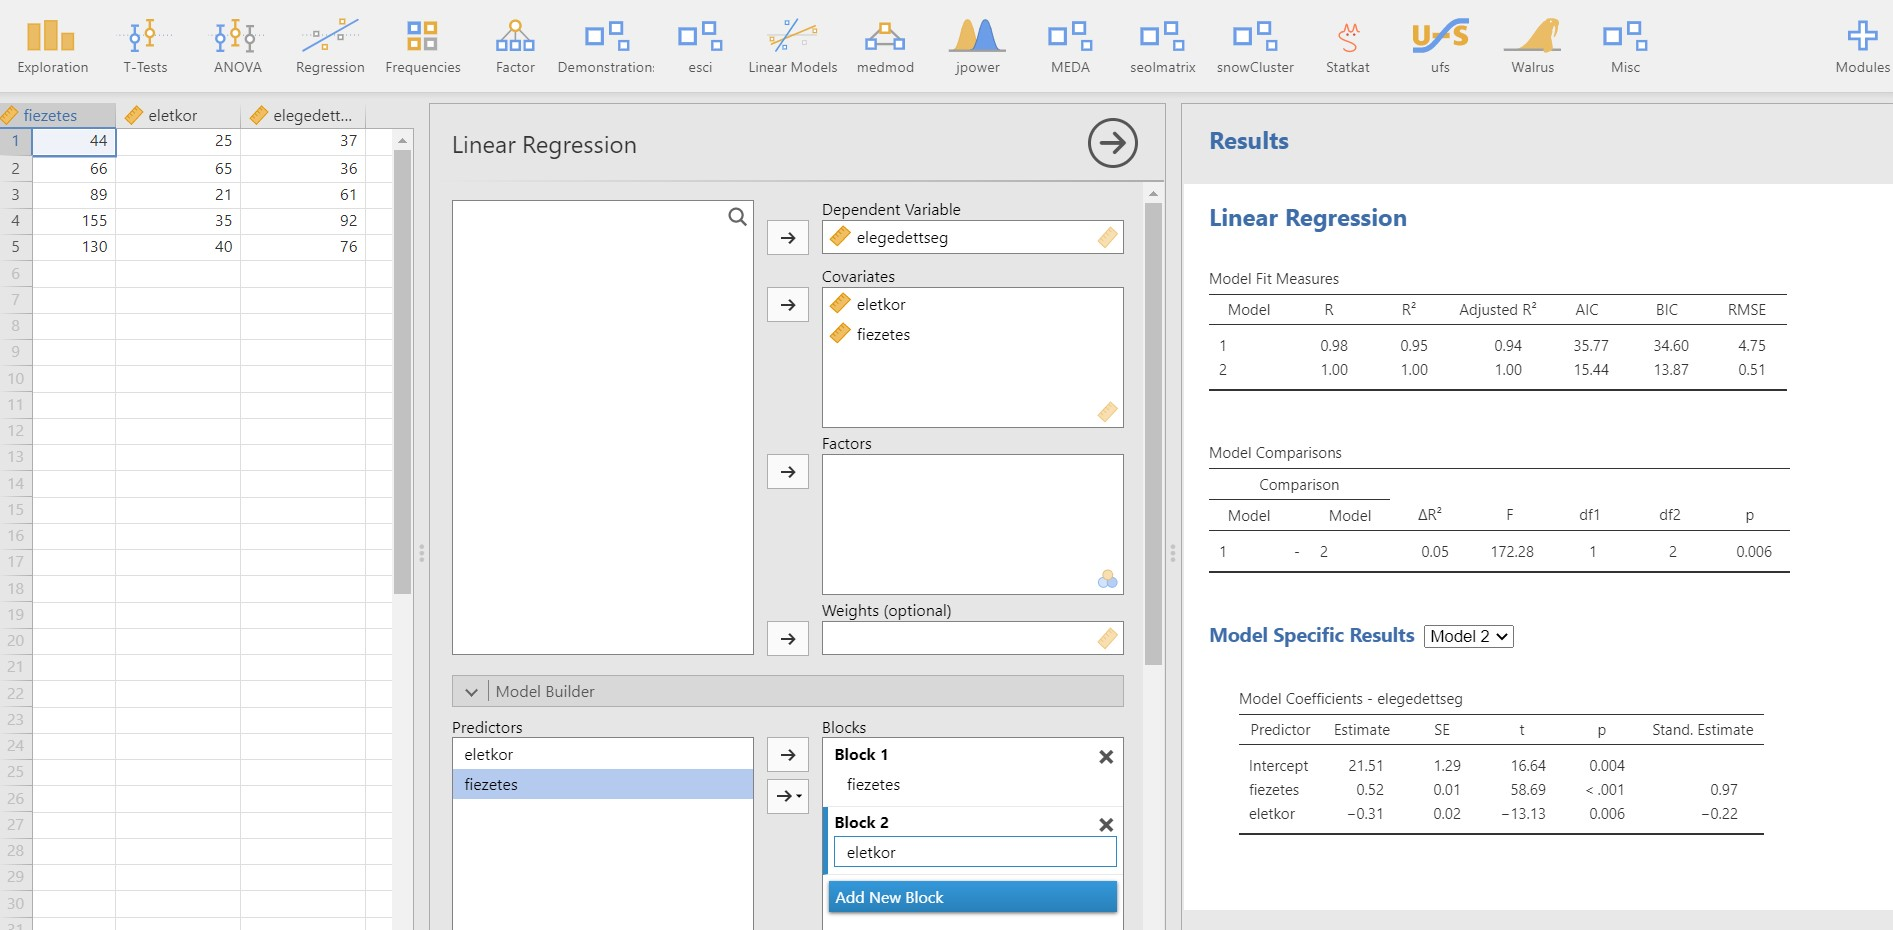
\includegraphics{./images/lin_reg_fizetes_eletkor_elegedettseg_01_kep_05.jpg}

}

\caption{Elégedettség kapcsolata a fizetéssel és az élekorral (N=5):
modellek összehasonlítása}

\end{figure}

A fenti példán látható, hogy két modellt építettünk. Az 1. modell az
elégedettséget a fizetés segítségével próbálja jósolni. A 2. modell az
elégedettséget a fizetéssel és az életkorral. Láthatjuk a 2. modell
szignifikánsan eltér magyarázó erőben a az 1. modelltől, valamint a
modell ``jóságát'' leíró mutatók mindegyike kedvezőbb a 2. modell
esetén: \(R_{adj}^2\), \(AIC\), \(BIC\), \(RMSE\).

\hypertarget{alkalmazuxe1si-feltuxe9telek}{%
\section{Alkalmazási feltételek}\label{alkalmazuxe1si-feltuxe9telek}}

A regressziós modellt ne használjuk, ha az alkalmazási feltételek
valamelyike nem teljesül. Melyek ezek?

\begin{itemize}
\tightlist
\item
  Multikollinearitás: a független változók közötti korreláció.
  Multikollinearitás esetén elképzelhető, hogy a regressziós számítást
  el sem lehet végezni. Van mérőszám, amelynek a segítségével ki lehet
  szűrni az érintett változókat:

  \begin{itemize}
  \tightlist
  \item
    VIF (variancia infláció faktor): a nagy érték kollinearitást jelez
    az érintett változókat kihagyhatjuk, vagy származtatott adatokkal
    dolgozunk tovább (például főkomponenselemzéssel nyert adatokat)
  \end{itemize}
\item
  Autokorreláció: a hibatagok együttmozgása szignifikáns.
\end{itemize}

\hypertarget{puxe9lda}{%
\section{1. Példa}\label{puxe9lda}}

Befolyásolja-e a munkahellyel való elégedettséget a fizetés nagysága és
az életkor? (Münnich és mtsai., 2006) {[}1.6.1 probléma{]}

\begin{Shaded}
\begin{Highlighting}[]
\NormalTok{d }\OtherTok{\textless{}{-}}\NormalTok{ rio}\SpecialCharTok{::}\FunctionTok{import}\NormalTok{(}\AttributeTok{file =} \StringTok{"adat/lin\_reg\_elegedettseg.xlsx"}\NormalTok{)}
\FunctionTok{str}\NormalTok{(d)}
\CommentTok{\#\textgreater{} \textquotesingle{}data.frame\textquotesingle{}:    30 obs. of  4 variables:}
\CommentTok{\#\textgreater{}  $ fizetes     : num  109 125 98 124 115 132 124 99...}
\CommentTok{\#\textgreater{}  $ elegedettseg: num  69.2 90.8 71 90.1 77.8 ...}
\CommentTok{\#\textgreater{}  $ kor         : num  20 46.3 36.2 46 31 ...}
\CommentTok{\#\textgreater{}  $ nem         : chr  "nő" "férfi" "nő" "férfi" ...}
\NormalTok{psych}\SpecialCharTok{::}\FunctionTok{headTail}\NormalTok{(d)}
\CommentTok{\#\textgreater{}     fizetes elegedettseg   kor   nem}
\CommentTok{\#\textgreater{} 1       109        69.15    20    nő}
\CommentTok{\#\textgreater{} 2       125        90.85 46.33 férfi}
\CommentTok{\#\textgreater{} 3        98        71.04  36.2    nő}
\CommentTok{\#\textgreater{} 4       124        90.12 45.95 férfi}
\CommentTok{\#\textgreater{} ...     ...          ...   ...  \textless{}NA\textgreater{}}
\CommentTok{\#\textgreater{} 27      129        96.32    53 férfi}
\CommentTok{\#\textgreater{} 28      135        97.86  49.4 férfi}
\CommentTok{\#\textgreater{} 29      145          100  46.9 férfi}
\CommentTok{\#\textgreater{} 30      120        81.08    32 férfi}
\end{Highlighting}
\end{Shaded}

\begin{Shaded}
\begin{Highlighting}[]
\NormalTok{lm\_1 }\OtherTok{\textless{}{-}} \FunctionTok{lm}\NormalTok{(elegedettseg }\SpecialCharTok{\textasciitilde{}}\NormalTok{ fizetes }\SpecialCharTok{+}\NormalTok{ kor, }\AttributeTok{data =}\NormalTok{ d)}
\FunctionTok{summary}\NormalTok{(lm\_1)}
\CommentTok{\#\textgreater{} }
\CommentTok{\#\textgreater{} Call:}
\CommentTok{\#\textgreater{} lm(formula = elegedettseg \textasciitilde{} fizetes + kor, data = d)}
\CommentTok{\#\textgreater{} }
\CommentTok{\#\textgreater{} Residuals:}
\CommentTok{\#\textgreater{}     Min      1Q  Median      3Q     Max }
\CommentTok{\#\textgreater{} {-}10.248  {-}1.543   1.188   2.437   4.333 }
\CommentTok{\#\textgreater{} }
\CommentTok{\#\textgreater{} Coefficients:}
\CommentTok{\#\textgreater{}             Estimate Std. Error t value Pr(\textgreater{}|t|)    }
\CommentTok{\#\textgreater{} (Intercept)  8.13712    3.26797   2.490   0.0192 *  }
\CommentTok{\#\textgreater{} fizetes      0.44404    0.02321  19.128  \textless{} 2e{-}16 ***}
\CommentTok{\#\textgreater{} kor          0.53361    0.07127   7.487 4.71e{-}08 ***}
\CommentTok{\#\textgreater{} {-}{-}{-}}
\CommentTok{\#\textgreater{} Signif. codes:  }
\CommentTok{\#\textgreater{} 0 \textquotesingle{}***\textquotesingle{} 0.001 \textquotesingle{}**\textquotesingle{} 0.01 \textquotesingle{}*\textquotesingle{} 0.05 \textquotesingle{}.\textquotesingle{} 0.1 \textquotesingle{} \textquotesingle{} 1}
\CommentTok{\#\textgreater{} }
\CommentTok{\#\textgreater{} Residual standard error: 3.59 on 27 degrees of freedom}
\CommentTok{\#\textgreater{} Multiple R{-}squared:  0.953,  Adjusted R{-}squared:  0....}
\CommentTok{\#\textgreater{} F{-}statistic: 273.9 on 2 and 27 DF,  p{-}value: \textless{} 2.2e{-}16}
\NormalTok{lsr}\SpecialCharTok{::}\FunctionTok{standardCoefs}\NormalTok{(lm\_1)}
\CommentTok{\#\textgreater{}                 b      beta}
\CommentTok{\#\textgreater{} fizetes 0.4440418 0.8322319}
\CommentTok{\#\textgreater{} kor     0.5336111 0.3257287}
\end{Highlighting}
\end{Shaded}

\begin{figure}

{\centering 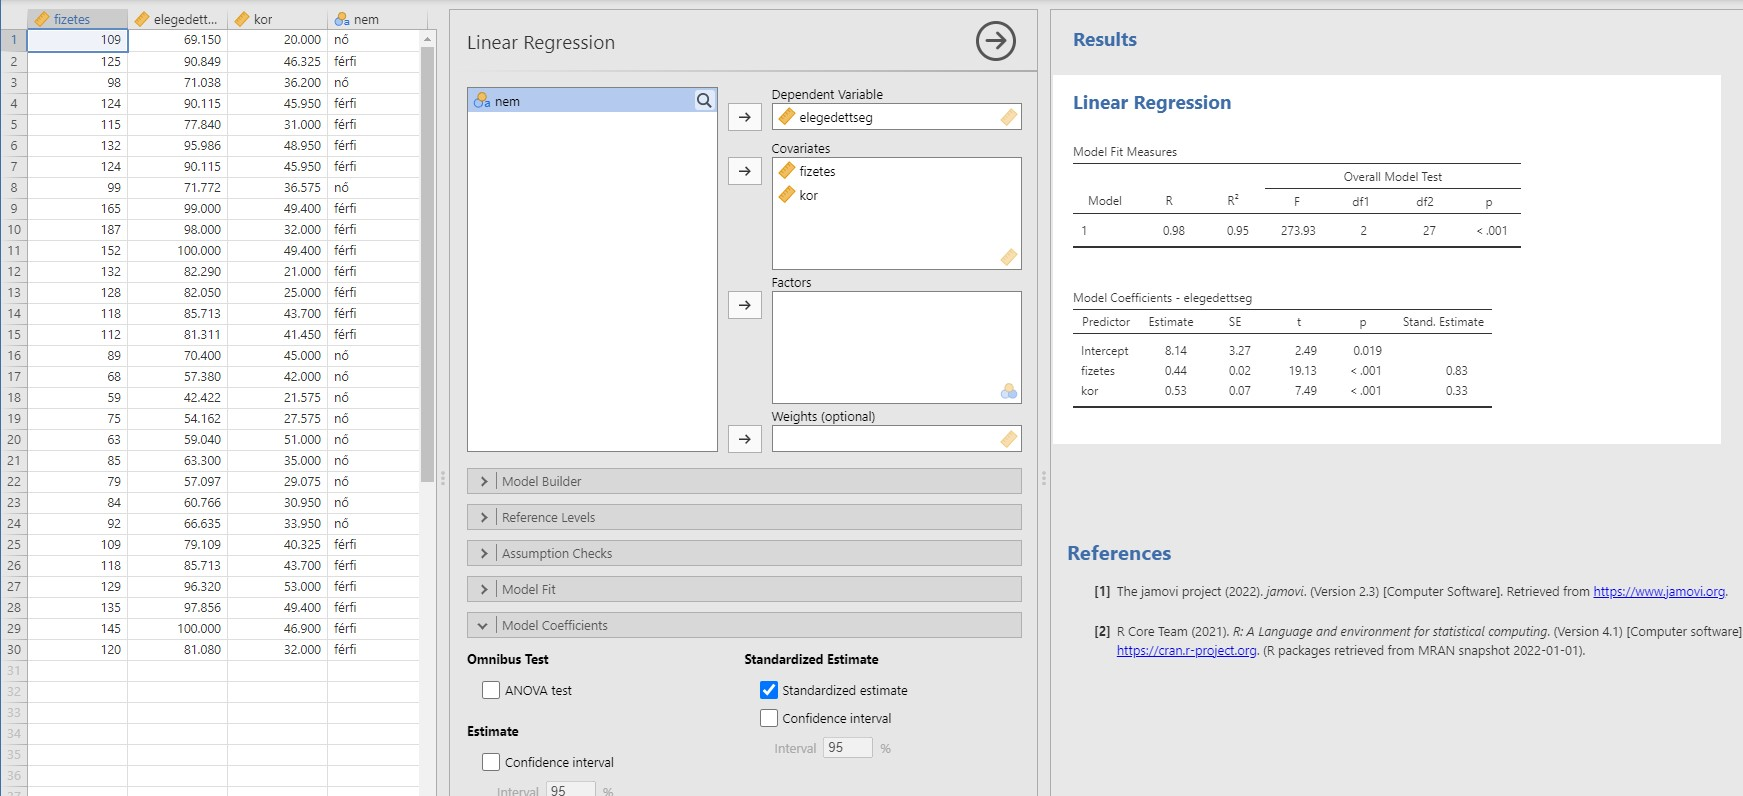
\includegraphics{./images/lin_reg_elegedettseg_kep_01.jpg}

}

\caption{Elégedettség kapcsolata a fizetéssel és lektkorra (N=30)}

\end{figure}

A fenti outputból láthatjuk, hogy a fizetés és a kor változó is
szignifikánsan befolyásolja az elégedettséget, hiszen a hozzájuk tartozó
szignifikanciaszint \(p<0,05\). A teljes modell vonatkozó F-próba is
szignifikáns. A fizetés változó együtthatója \((b_1)\) 0,44, a kor
változó együtthatója \((b_2)\) pedig 0,53, ami arra utal, hogy pozitív
kapcsolat van a változó között: minél magasabb a fizetés, és minél
idősebbek az emberek, annál elégedettebbek a munkahelyükkel.

A pontos becslés a regressziós egyenlet alapján a következőképpen fest:

\begin{Shaded}
\begin{Highlighting}[]
\NormalTok{elégedettség = 8,14 + 0,44 * fizetés + 0,53 * kor}
\end{Highlighting}
\end{Shaded}

Mivel a többszörös regresszió esetében a független változók hatása csak
a standardizált együtthatók mentén hasonlítható össze, így kiszámoltuk a
standardizált együtthatókat is. Az adatok jól példázzák, hogy miért
fontos a standardizált együtthatókat is vizsgálni, hiszen a nem
standardizált együtthatók esetén a kor változó együtthatójának értéke a
magasabb, míg a standardizált értékeknél fordítva. Vagyis, ha az egyes
változók relatív fontosságának vizsgálatakor nem nézzük a dimenziómentes
értékeket, akkor könnyen téves következtetésre juthatunk.

A négyzetes korrelációs együttható értéke 0,9, ami arra utal, hogy a
független változók igen jól magyarázzák a függő változót.

\hypertarget{puxe9lda-1}{%
\section{2. Példa}\label{puxe9lda-1}}

Befolyásolja-e a kalandvágy a hivatásos katonai szolgálatnál eltöltött
időt? (Münnich és mtsai., 2006) {[}1.6.2 probléma{]}

\begin{Shaded}
\begin{Highlighting}[]
\NormalTok{d }\OtherTok{\textless{}{-}}\NormalTok{ rio}\SpecialCharTok{::}\FunctionTok{import}\NormalTok{(}\AttributeTok{file =} \StringTok{"adat/lin\_reg\_katonasag.xlsx"}\NormalTok{)}
\FunctionTok{str}\NormalTok{(d)}
\CommentTok{\#\textgreater{} \textquotesingle{}data.frame\textquotesingle{}:    156 obs. of  4 variables:}
\CommentTok{\#\textgreater{}  $ kaland  : num  3 3 5 1 3 4 2 2 3 5 ...}
\CommentTok{\#\textgreater{}  $ egyhangu: num  3 2 4 1 3 1 2 1 2 3 ...}
\CommentTok{\#\textgreater{}  $ sport   : num  1 1 2 1 2 2 2 1 2 2 ...}
\CommentTok{\#\textgreater{}  $ evek    : num  4 7 10 3 6 15 5 6 9 13 ...}
\NormalTok{psych}\SpecialCharTok{::}\FunctionTok{headTail}\NormalTok{(d)}
\CommentTok{\#\textgreater{}     kaland egyhangu sport evek}
\CommentTok{\#\textgreater{} 1        3        3     1    4}
\CommentTok{\#\textgreater{} 2        3        2     1    7}
\CommentTok{\#\textgreater{} 3        5        4     2   10}
\CommentTok{\#\textgreater{} 4        1        1     1    3}
\CommentTok{\#\textgreater{} ...    ...      ...   ...  ...}
\CommentTok{\#\textgreater{} 153      2        4     2    1}
\CommentTok{\#\textgreater{} 154      3        5     3    2}
\CommentTok{\#\textgreater{} 155      1        3     2    2}
\CommentTok{\#\textgreater{} 156      3        2     4   12}
\end{Highlighting}
\end{Shaded}

\begin{Shaded}
\begin{Highlighting}[]
\NormalTok{lm\_1 }\OtherTok{\textless{}{-}} \FunctionTok{lm}\NormalTok{(evek }\SpecialCharTok{\textasciitilde{}}\NormalTok{ egyhangu }\SpecialCharTok{+}\NormalTok{ sport }\SpecialCharTok{+}\NormalTok{ kaland, }\AttributeTok{data =}\NormalTok{ d)}
\FunctionTok{summary}\NormalTok{(lm\_1)}
\CommentTok{\#\textgreater{} }
\CommentTok{\#\textgreater{} Call:}
\CommentTok{\#\textgreater{} lm(formula = evek \textasciitilde{} egyhangu + sport + kaland, data...}
\CommentTok{\#\textgreater{} }
\CommentTok{\#\textgreater{} Residuals:}
\CommentTok{\#\textgreater{}     Min      1Q  Median      3Q     Max }
\CommentTok{\#\textgreater{} {-}1.6611 {-}0.5925 {-}0.0798  0.2726  9.7833 }
\CommentTok{\#\textgreater{} }
\CommentTok{\#\textgreater{} Coefficients:}
\CommentTok{\#\textgreater{}             Estimate Std. Error t value Pr(\textgreater{}|t|)    }
\CommentTok{\#\textgreater{} (Intercept)  0.63951    0.33263   1.923   0.0564 .  }
\CommentTok{\#\textgreater{} egyhangu    {-}2.28197    0.09160 {-}24.912   \textless{}2e{-}16 ***}
\CommentTok{\#\textgreater{} sport        1.52987    0.09447  16.194   \textless{}2e{-}16 ***}
\CommentTok{\#\textgreater{} kaland       3.17525    0.09884  32.125   \textless{}2e{-}16 ***}
\CommentTok{\#\textgreater{} {-}{-}{-}}
\CommentTok{\#\textgreater{} Signif. codes:  }
\CommentTok{\#\textgreater{} 0 \textquotesingle{}***\textquotesingle{} 0.001 \textquotesingle{}**\textquotesingle{} 0.01 \textquotesingle{}*\textquotesingle{} 0.05 \textquotesingle{}.\textquotesingle{} 0.1 \textquotesingle{} \textquotesingle{} 1}
\CommentTok{\#\textgreater{} }
\CommentTok{\#\textgreater{} Residual standard error: 1.213 on 152 degrees of fr...}
\CommentTok{\#\textgreater{} Multiple R{-}squared:  0.9195, Adjusted R{-}squared:  0...}
\CommentTok{\#\textgreater{} F{-}statistic: 578.4 on 3 and 152 DF,  p{-}value: \textless{} 2.2...}
\NormalTok{lsr}\SpecialCharTok{::}\FunctionTok{standardCoefs}\NormalTok{(lm\_1)}
\CommentTok{\#\textgreater{}                  b       beta}
\CommentTok{\#\textgreater{} egyhangu {-}2.281974 {-}0.5927751}
\CommentTok{\#\textgreater{} sport     1.529871  0.3821476}
\CommentTok{\#\textgreater{} kaland    3.175249  0.7676009}
\end{Highlighting}
\end{Shaded}

\begin{figure}

{\centering 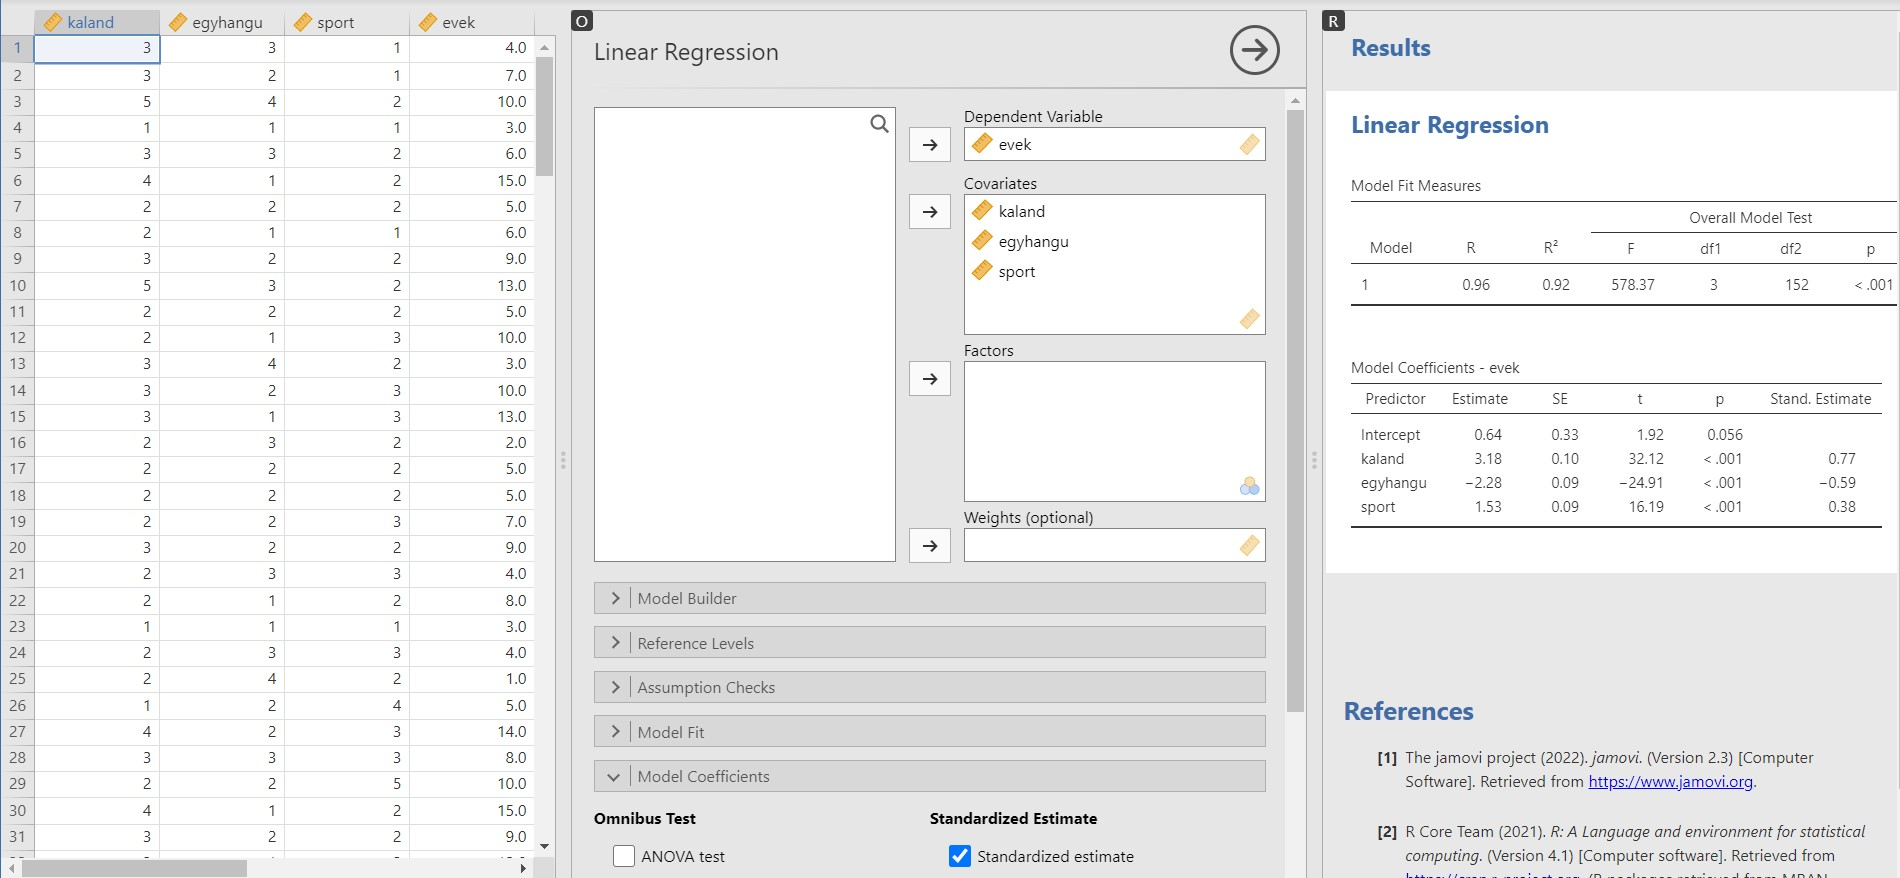
\includegraphics{./images/lin_reg_katonasag_kep_01.jpg}

}

\caption{Befolyásolja-e a kalandvágy a hivatásos katonai szolgálatnál
eltöltött időt? (N=156)}

\end{figure}

A fenti output a többszörös lineáris regresszió eredményét mutatja:

\begin{itemize}
\tightlist
\item
  A lineáris regressziós modellt megtarthatjuk, hiszen az F-statisztika
  értékét tekintve a modell szignifikáns, a változók együtthatóinak az
  értéke nem nulla.
\item
  A modell magyarázóértéke igen jó, hiszen a korrigált determinációs
  együttható értéke 0,92, vagyis a független változók a függő változó
  varianciájának kb. 92\%-át magyarázzák.
\item
  Minden egyes független változó hatással van a függő változóra, vagyis
  mind a kalandvágy, az extrém sportok szeretete és a nyugalom utáni
  vágy is befolyásolja azt, hogy mennyi időt tölt valaki a hivatásos
  katonai szolgálatban.
\item
  Ellenben a \(b_0\) vagyis a konstans értéke most nulla, hiszen a
  táblázatban szereplő érték nem szignifikáns.
\item
  Maga a regressziós egyenlet a pontos együtthatók ismeretében a
  következőképpen alakul:
\end{itemize}

\begin{Shaded}
\begin{Highlighting}[]
\InformationTok{    evek=3,18*kaland+1,53*sport{-}2,28*egyhangu}
\end{Highlighting}
\end{Shaded}

\begin{itemize}
\item
  Vagyis minél jobban kedveli valaki a kalandos életet és az extrém
  sportokat, és minél jobban irtózik a szürke hétköznapoktól, annál több
  időt tölt a katonaság kötelékében.
\item
  A standardizált változók alapján a kaland szeretetének a hatása a
  legerősebb (0,768), a második legerősebb hatás az egyhangúság
  kedvelése, ám hatásának iránya negatív (-0,593), leggyengébb hatása
  pedig az extrém sportok szeretetének van (0,382).
\end{itemize}

\bookmarksetup{startatroot}

\hypertarget{sec-fokomponens-elemzes}{%
\chapter{Főkomponens elemzés}\label{sec-fokomponens-elemzes}}

A főkomponens elemzés a legegyszerűbb többváltozós statisztikai
eljárások egyike. Olyan eljárás, amely az egy jelenségre vonatkozó
méréseket úgy „összegzi'', hogy közben az óhatatlanul fellépő információ
veszteséget a lehető legkisebb mértékűre csökkenti.

A módszer alapgondolata az, hogy vegyünk \(p\) változót:
\(X_1,X_2,\dots,X_p\), majd keressük meg ezek kombinációit, hogy ezáltal
\(Z_1,Z_2,..,Z_p\)-vel jelölt indexeket kaphassunk, melyek egymással nem
korrelálnak, továbbá
\(var(Z_1 )\geq var(Z_2 )\geq \dots \geq var(Z_p)\), ahol \(var(Z_i)\) a
\(Z_i\) komponens varianciáját jelöli.

A korreláció hiánya a \(Z_i\)-kben hasznos tulajdonság, ugyanis azt
jelenti, hogy az indexek az adatok különböző ``dimenzióit'' mérik.

A \(Z_i\)-t főkomponensnek nevezzük. Amikor főkomponens-analízist
végzünk, mindig abban bízunk, hogy a legtöbb index varianciája
elhanyagolhatóan kicsi. Ezáltal az adatok varianciája adekvátan leírható
néhány olyan \(Z_i\) változóval, melyek varianciája nem elhanyagolható.

A főkomponens analízis működéséhez szükséges, hogy az eredeti
\(X_1,X_2,\dots,X_p\) változók korreláljanak egymással (akár pozitív,
akár negatív irányban), ekkor elképzelhető az az eset, hogy 20-30
eredeti változót adekvátan reprezentálhat 2-3 főkomponens. Ha pedig ez
teljesül, akkor a fontosabb főkomponensek (melyek varianciája elég nagy)
lesznek csupán érdekesek, hiszen ezek fogják az adatok „dimenzióit''
mérni. Természetesen nagyon fontos azt is tudnunk, hogy rengeteg eredeti
változónk van, és legtöbbjük ugyanazt, vagy legalábbis hasonló dolgokat
mér.

\hypertarget{a-fux151komponens-elemzuxe9s-menete}{%
\section{A főkomponens elemzés
menete}\label{a-fux151komponens-elemzuxe9s-menete}}

Az eredeti \(X_1,X_2,\dots,X_p\) változókból a
\(Z_i=a_i1 X_1+ a_i2 X_2+\dots + a_ip X_p\) lineáris kombinációk
segítségével kapjuk meg a főkomponenseket, azzal feltétellel, hogy
\(a_{i1}^2+a_{i2}^2+\dots+a_{ip}^2=1\), és az egymás után létrejövő
\(Z_1,Z_2,…,Z_p\) főkomponensek nem korrelálnak egymással.

Gyakran az \(X_1,X_2,\dots,X_p\) változó standardizált értékeiből
indulunk ki, hogy a változók arányosan fejtsék ki hatásukat a
főkomponensekre. A jamovi is így végzi az elemzést. Ekkor a változok
átlaga nulla, szórása és variancia pedig 1 lesz.

A részletek ismertetése nélkül a keresett \(a_{i1},a_{i2},\dots,a_{ip}\)
együtthatók megtalálása egy sajátérték-sajátvektor keresési feladat az
eredeti \(X_1,X_2,\dots,X_p\) változók korrelációs mátrixában. A
megtalált \(p\) darab sajátérték
\$\lambda\_1\geq\lambda\_2\geq\dots\geq\lambda\_p\textgreater0
\$sorrendjét feltételezve, \(\lambda_i\) az \(i.\) főkomponens
varianciáját adja \((\lambda_i=var(Z_i))\), és a megtalált \(p\) darab
sajátvektorból az \(i.\) egyes elemei lesznek a
\(Z_i=a_{i1} X_1+ a_{i2} X_2+\dots+ a_{ip} X_p\) főkomponens
\(a_{i1},a_{i2},\dots,a_{ip}\) együtthatói.

Fontos összefüggés, hogy a főkomponensek (\(Z_i\)-k) varianciájának az
összege egyenlő az eredeti standardizált változók (\(X_i\)-k)
varianciájának összegével, azaz
\(\lambda_1+\lambda_2+\dots+\lambda_p=1+1+\dots+1=p.\)

\hypertarget{a-fux151komponens-elemzuxe9s-alkalmazuxe1si-feltuxe9telei}{%
\section{A főkomponens elemzés alkalmazási
feltételei}\label{a-fux151komponens-elemzuxe9s-alkalmazuxe1si-feltuxe9telei}}

\begin{itemize}
\tightlist
\item
  A főkomponens elemzés során általában 4-5-ször (egyes szerzőknél
  10-szer) nagyobb a mintaelemszám a vizsgált változók számánál.
\item
  A faktoranalízis feltétele, hogy egymással korreláló változókból
  induljunk ki. A Bartlett-féle szferikus próba nullhipotézise, hogy a
  változók korrelálatlanok (vagyis a korrelációs mátrixnak a főátlón
  kívüli elemei csak véletlenül térnek el a nullától). A szignifikáns
  p-érték a kedvező a főkomponens elemzés számára. (Megjegyezzük, hogy a
  túlságosan magas egyirányú korrelációk sem jók, ugyanis ez azt
  okozhatja, hogy a főkomponens elemzésnek nem lesz megoldása, ugyanis
  minden változó egy faktorba kerül.)
\item
  Az MSA (Measure of Sampling Adequecy) az egyes változók esetében
  mutatja meg, hogy mennyire van szoros kapcsolatban a többi változóval.
  Érdemes a 0,5 alatti MSA értékkel rendelkező változókat kizárni az
  elemzésből. Értéke 0 és 1 közötti lehet.
\item
  A Kaiser-Meyer-Olkin- (KMO) kritérium az MSA értékek átlaga. Míg az
  MSA érték az egyes változókra vonatkozik, a KMO az összes változóra
  egyidejűleg. A KMO mutatószám jelentését a következőképpen ítélhetjük
  meg:

  \begin{itemize}
  \tightlist
  \item
    KMO ≥ 0,9 kiváló
  \item
    KMO ≥ 0,8 nagyon jó
  \item
    KMO ≥ 0,7 megfelelő
  \item
    KMO ≥ 0,6 közepes
  \item
    KMO ≥ 0,5 gyenge
  \item
    KMO \textless{} 0,5 elfogadhatatlan.
  \end{itemize}
\end{itemize}

\hypertarget{a-fux151komponensek-forgatuxe1sa-rotuxe1ciuxf3}{%
\section{A főkomponensek forgatása
(rotáció)}\label{a-fux151komponensek-forgatuxe1sa-rotuxe1ciuxf3}}

A faktorkiválasztás (extrakció) során az elemzés elsődleges célja, hogy
maximalizálja a főkomponensek varianciáját, amely eredményeként
megkapjuk a rotálatlan faktorsúly-mátrixot. A faktorsúly az eredeti
változó és az adott faktor közötti korrelációt mutatja, amelynek értéke
a korrelációs együtthatókhoz hasonlóan -1 és 1 között változhat.

A faktorkiválasztás során azonban előfordulhat, hogy olyan változók
fognak korrelálni egy adott faktorral, amelyeknek semmi közük egymáshoz,
ezáltal lehetetlenné téve az értelmezést. Ezen a problémán segít a
forgatás, vagy más néven rotáció. A faktor-rotáció azt jelenti, hogy a
faktorok tengelyeit elforgatjuk úgy, hogy egyszerűbb és értelmezhetőbb
faktormegoldáshoz vezessen.

A rotáció (forgatás) során nem változnak sem a kommunalitás, sem pedig
az összes magyarázott variancia, csak a faktorok
sajátértékei/magyarázott varianciái módosulnak.

A rotáláson belül két típust különböztetünk meg: a derékszögű
(ortogonális) (Varimax, Equimax, Quartimax) és a hegyesszögű (nem
ortogonális) (Direct Oblimin, Promax) forgatási módszereket.

A derékszögű esetében a tengelyek merőlegesen állnak egymásra, ezáltal a
faktorok nem korrelálnak egymással, míg a hegyesszögű esetében ezek
tetszőleges szöget zárnak be egymással, vagyis a faktorok korrelálni
fognak egymással.

\hypertarget{puxe9lda-2}{%
\section{1. Példa}\label{puxe9lda-2}}

A példa Münnich és mtsai. (2006) 2.3.1. alfejezet alapján készült és a
kapcsolódó jamovi állomány: \texttt{fokomp\_elemzes\_tantargyak.omv}.

\textbf{1. Határozzuk meg a korrelációs mátrixot (jamovi-ban:
\texttt{Regression\ /\ Correlation\ matrix})}

\begin{Shaded}
\begin{Highlighting}[]
\NormalTok{d }\OtherTok{\textless{}{-}}\NormalTok{ rio}\SpecialCharTok{::}\FunctionTok{import}\NormalTok{(}\AttributeTok{file =} \StringTok{"adat/fokomp\_elemzes\_tantargyak.xlsx"}\NormalTok{)}
\FunctionTok{str}\NormalTok{(d)}
\CommentTok{\#\textgreater{} \textquotesingle{}data.frame\textquotesingle{}:    9 obs. of  4 variables:}
\CommentTok{\#\textgreater{}  $ matek      : num  5 4 3 2 5 1 5 2 5}
\CommentTok{\#\textgreater{}  $ fizika     : num  5 5 3 3 4 2 4 3 5}
\CommentTok{\#\textgreater{}  $ informatika: num  4 4 4 2 5 1 5 2 5}
\CommentTok{\#\textgreater{}  $ kemia      : num  5 5 3 3 5 1 5 3 5}
\NormalTok{d}
\CommentTok{\#\textgreater{}   matek fizika informatika kemia}
\CommentTok{\#\textgreater{} 1     5      5           4     5}
\CommentTok{\#\textgreater{} 2     4      5           4     5}
\CommentTok{\#\textgreater{} 3     3      3           4     3}
\CommentTok{\#\textgreater{} 4     2      3           2     3}
\CommentTok{\#\textgreater{} 5     5      4           5     5}
\CommentTok{\#\textgreater{} 6     1      2           1     1}
\CommentTok{\#\textgreater{} 7     5      4           5     5}
\CommentTok{\#\textgreater{} 8     2      3           2     3}
\CommentTok{\#\textgreater{} 9     5      5           5     5}
\end{Highlighting}
\end{Shaded}

\begin{Shaded}
\begin{Highlighting}[]
\FunctionTok{cor}\NormalTok{(d)}
\CommentTok{\#\textgreater{}                 matek    fizika informatika     kemia}
\CommentTok{\#\textgreater{} matek       1.0000000 0.8712476   0.9492623 0.9499475}
\CommentTok{\#\textgreater{} fizika      0.8712476 1.0000000   0.7662496 0.9271176}
\CommentTok{\#\textgreater{} informatika 0.9492623 0.7662496   1.0000000 0.8867155}
\CommentTok{\#\textgreater{} kemia       0.9499475 0.9271176   0.8867155 1.0000000}
\end{Highlighting}
\end{Shaded}

\begin{figure}

{\centering 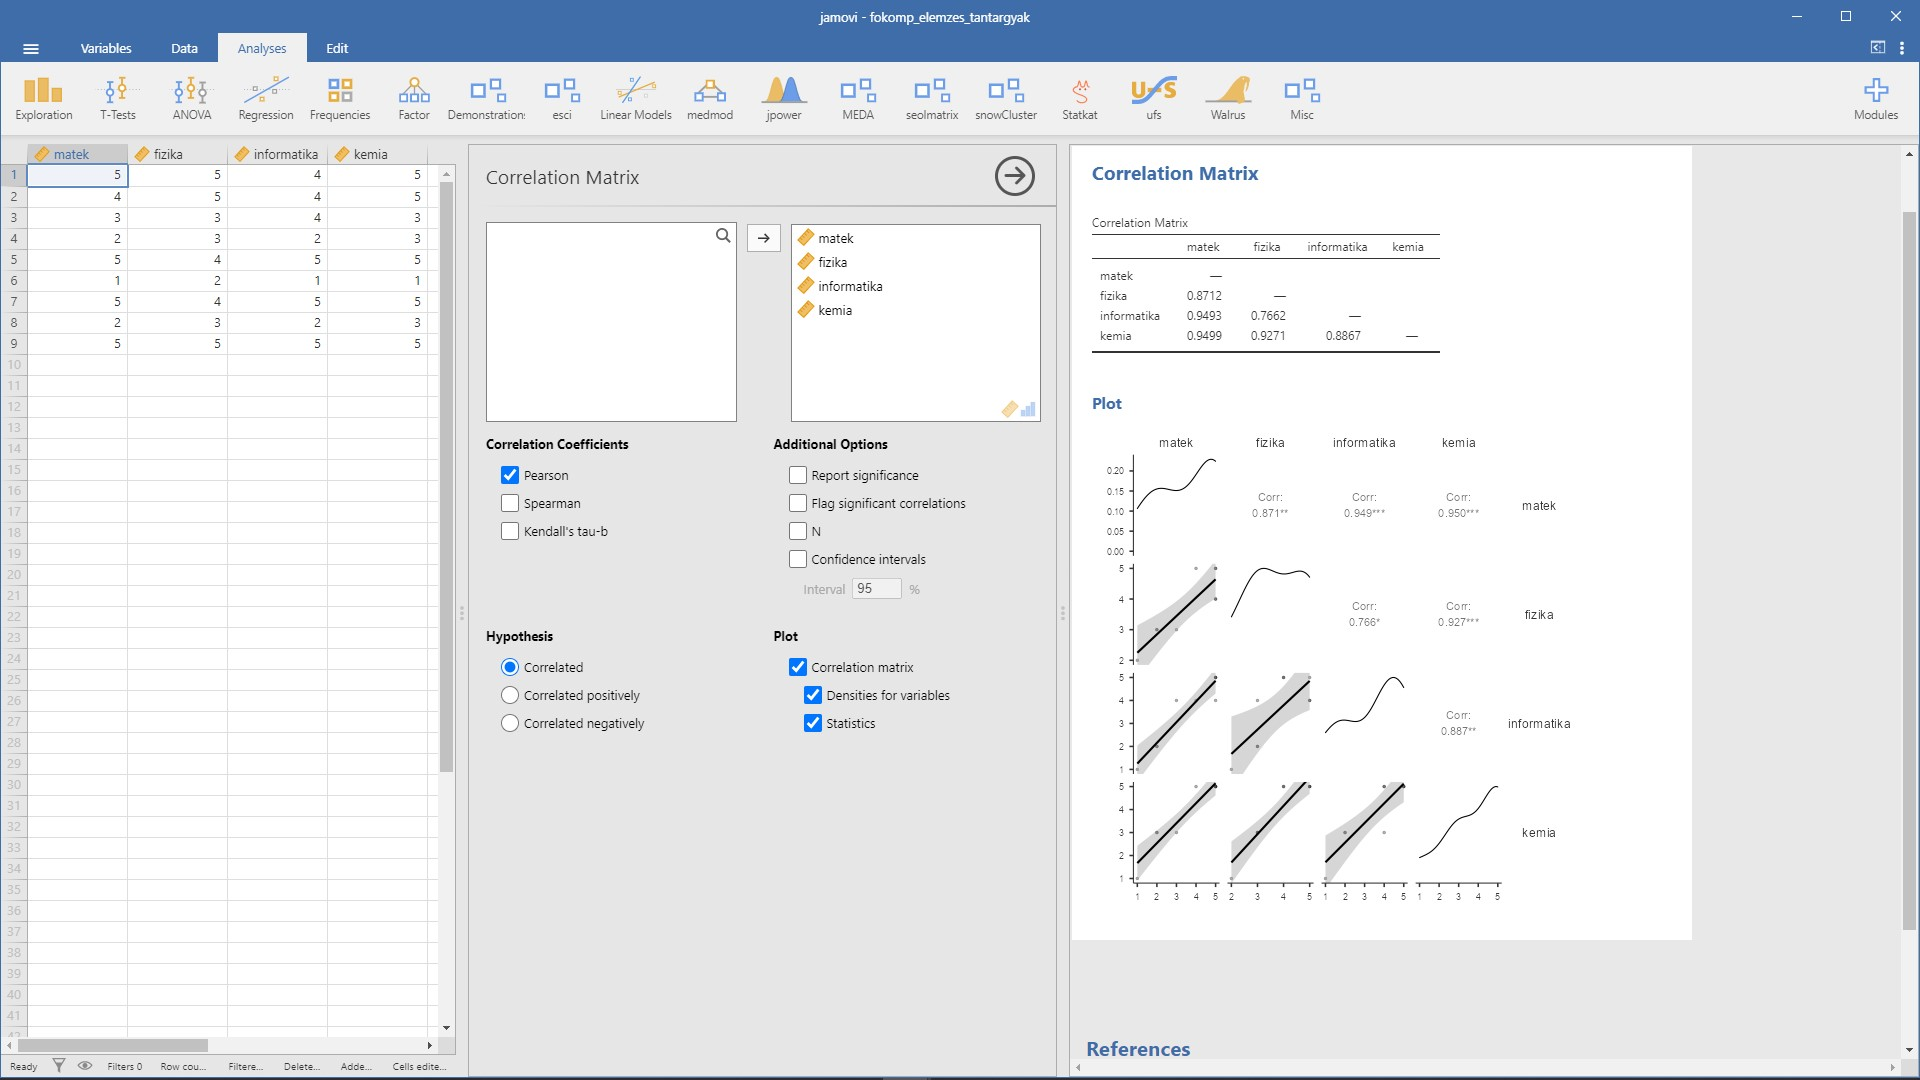
\includegraphics{./images/fokomponens_kep_01.jpg}

}

\caption{Korrelációs mátrix meghatározása}

\end{figure}

A korrelációs mátrix adatai arra utalnak, hogy szoros kapcsolat van a
változók között. A korrelációs értékek nullánál nagyobbak, ami azonos
irányú tendenciákra utal. E két mátrix is alátámasztja a
feltételezésünket, hogy a változók szorosan együtt változnak.

\textbf{2. Ellenőrizzük le az adatok alkalmasságát (jamovi-ban:
\texttt{Factor\ /\ Principal\ Component\ Analysis})}

A változóink eleget tesznek a Bartlett-féle szferikus próbának, a
korrelációs mátrix nem egységmátrix \((p<0,001)\), az MSA értékek is
nagyobban \(0,5\)-nél és a KMO érték is megfelelő.

\begin{figure}

{\centering 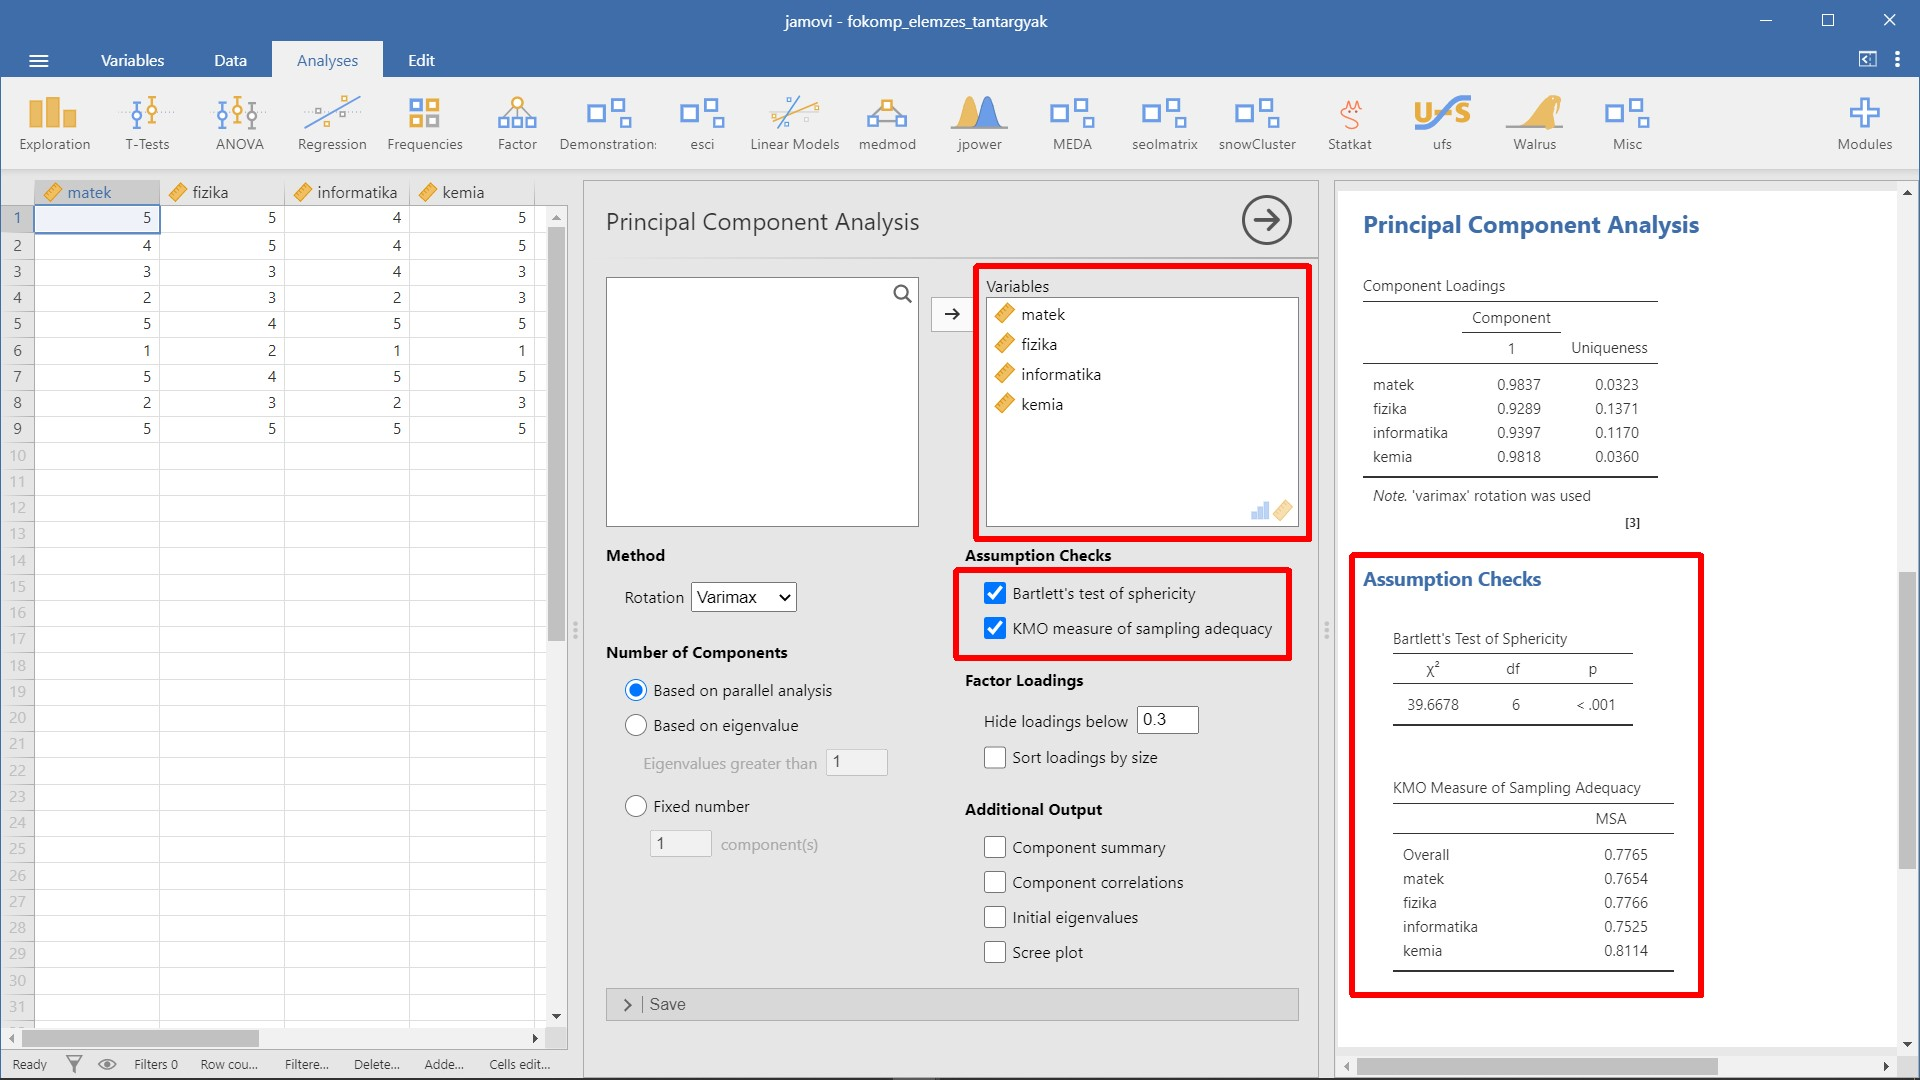
\includegraphics{./images/fokomponens_kep_02.jpg}

}

\caption{Alkalmazási feltételek ellenőrzése}

\end{figure}

\textbf{3. Határozzuk meg a komponensek számát}

Elvileg annyi főkomponenst lehet kiszámolni, ahány változónk van, a
célunk azonban a komponensek számának minimalizálása.

Több eljárás létezik a főkomponensek számának meghatározására:

\begin{itemize}
\tightlist
\item
  Horn-féle párhuzamos analízis (jamovi-ban:
  \texttt{Based\ on\ parallel\ analysis}): modern eljárás, amely
  szimuláció segítségével állapítja meg a főkomponensek számát (Horn,
  1965).
\item
  A priori meghatározás (jamovi-ban: \texttt{Fixed\ number}): korábbi
  ismerete alapján megadjuk a főkomponensek számát.
\item
  Sajátértéken alapuló megoldás (jamovi-ban:
  \texttt{Based\ on\ eigenvalue}): tipikusan csak az 1-nél nagyobb
  sajátértékű faktorokat tartjuk bent a modellben. Az 1-nél kisebb
  varianciájú faktorok ugyanis nem jobbak mint az eredeti standardizált
  változók
\item
  Sajátértékábrán (scree-plot, kőtörmelék ábra) alapuló meghatározás
  (jamovi-ban: \texttt{Scree\ plot}): a sajátérték ábra a sajátértékek
  ábrázolása a főkomponensek sorrendjében. Az ábra formája alapján lehet
  következtetni a főkomponensek számára: ahol a görbe meredekségében van
  egy határozott törés, meredekebb rész után laposabb jön. Ahol tehát a
  görbe laposodása elkezdődik, az a figyelembe vett főkomponensek
  megfelelő száma.
\item
  Magyarázott varianciahányadon alapuló meghatározás (jamovi-ban:
  \texttt{Component\ summary}): ekkor az előállított főkomponensek
  számát úgy határozzuk meg, hogy a főkomponensek által magyarázott
  variancia kumulált százalékos értéke elérjen egy megfelelő szintet. A
  megfelelő szint (60\%-95\%-ig) a probléma jellegétől függ.
\end{itemize}

A Horn-féle párhuzamos elemzés 1 főkomponenst javasol.

\begin{figure}

{\centering 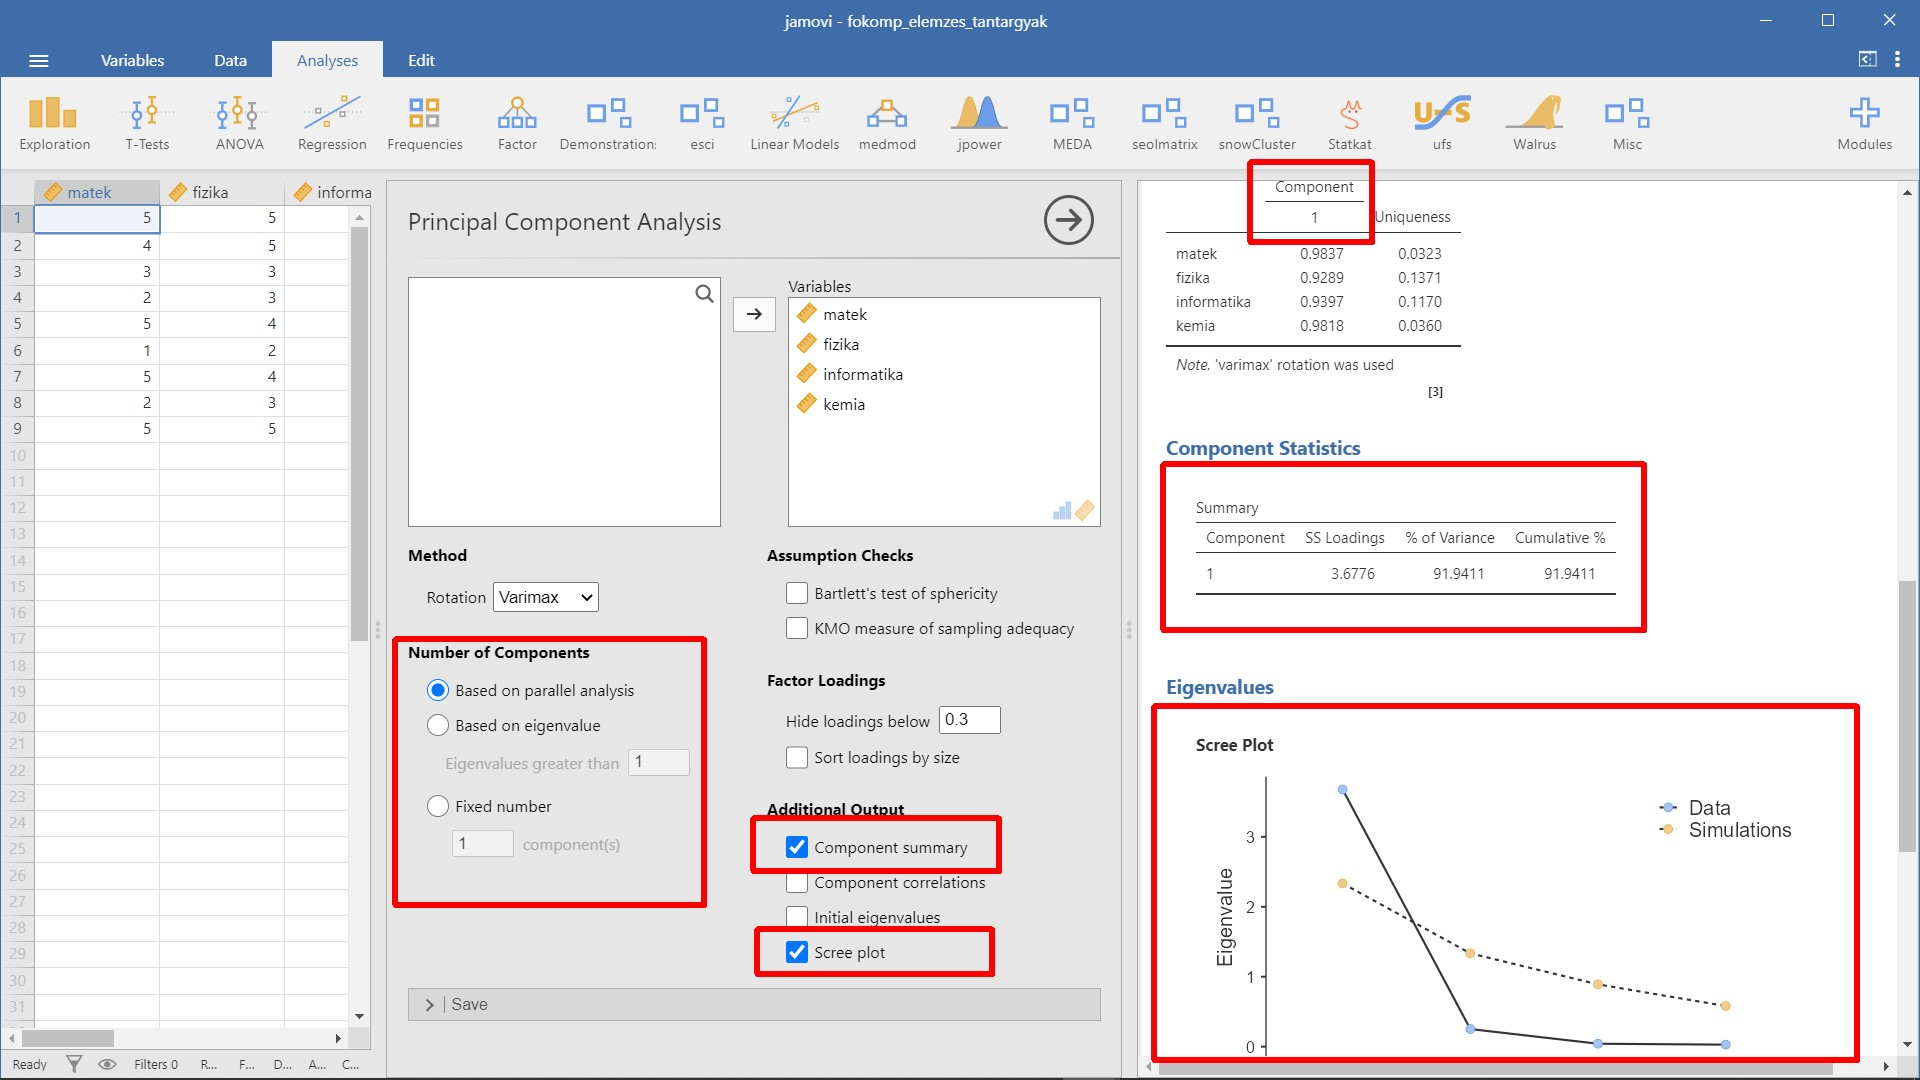
\includegraphics{./images/fokomponens_kep_03.jpg}

}

\caption{Főkomponensek számának meghatározása}

\end{figure}

\textbf{4. Válasszunk forgatást (jamovi-ban: \texttt{Rotation})}

A jamovi alapértelmezés szerint a Varimax forgatást ajánlja, amely
derékszögű koordinátatengelyeket eredményez és a legtöbb esetben ez a
megfelelő választás. Lehetőségünk van ezen módosítani. Az összes
lehetőség:

\begin{itemize}
\tightlist
\item
  None -- rotálatlan elemzés
\item
  Varimax
\item
  Qartimax
\item
  Promax
\item
  Oblimin
\item
  Simplimax
\end{itemize}

Mivel egyetlen főkomponensünk van, így nem változtatunk az
alapértelmezett Varimax beállításon.

\textbf{5. A főkomponens elemzés eredménye}

\emph{Komponens mátrix (jamoviban: \texttt{Component\ loadings})}

A főkomponens elemzés eredménye a komponens mátrix (faktormátrix),
amelynek soraiban az eredeti változók, oszlopaiban a kinyert
főkomponensek vannak. A cellákban a komponens súlyok (faktorsúlyok)
szerepelnek, amelyek a főkomponens és a változó közötti korrelációt
jelentik. Ezek egyben a főkomponensek azon együtthatói, amelyekkel a
standardizált változó a főkomponensekkel kifejezhető.

A magas abszolút értékű faktorsúly azt jelzi, hogy komponens és a
változó szorosan összefügg.

A változókat tartalmazó sorok rendezhetők a faktorsúlyok csökkenő
sorrendjében (jamovi-ban: \texttt{Sort\ loading\ by\ size})

Az adott értéknél kisebb faktorsúlyok elrejthetők a táblázatban
(jamoviban: \texttt{Hide\ loadings\ below})

A \texttt{Uniqueness} oszlopban az egyes változók „egyediségét'' is
láthatjuk. Az egyediség a variancia azon aránya, amely „egyedi'' a
változóra nézve, és nem magyarázható a komponensekkel. Vegyük
figyelembe, hogy minél nagyobb az „egyediség'', annál kisebb a változó
relevanciája/hozzájárulása a modellben.

\emph{A kezdő sajátértékek (jamovi-ban: \texttt{Initial\ eigenvalues})}

A kezdő sajátértékek táblázat a sajátértékeket adja meg. A komponensek
sajátértékei csökkenő nagyságúak, ahogy az 1. komponenstől a 4.
komponensig haladunk. A komponens sajátértéke kifejezi a komponens által
magyarázott teljes varianciát. A 4 komponens összvarianciája pontosan 4.
A további két oszlopban ez alapján számoljuk a százalékos és a kummulált
százalékos varianciát.

\emph{A komponensek összegzése (jamovi-ban:
\texttt{Component\ summary})}

A komponensek összegzése táblázat tartalmazza a megtartott
komponenseket, a magyarázott varianciát, illetve utóbbit százalékosan is
kifejezve. Vegyük észre, hogy ez a sor teljesen megegyezik a kezdő
sajátértékek táblázat első sorával. Az \texttt{SS\ Loadings} felirat
magyarázata, hogy magyarázott variancia a komponenshez tartozó
faktorsúlyok négyzetösszege (sum of square).

\begin{figure}

{\centering 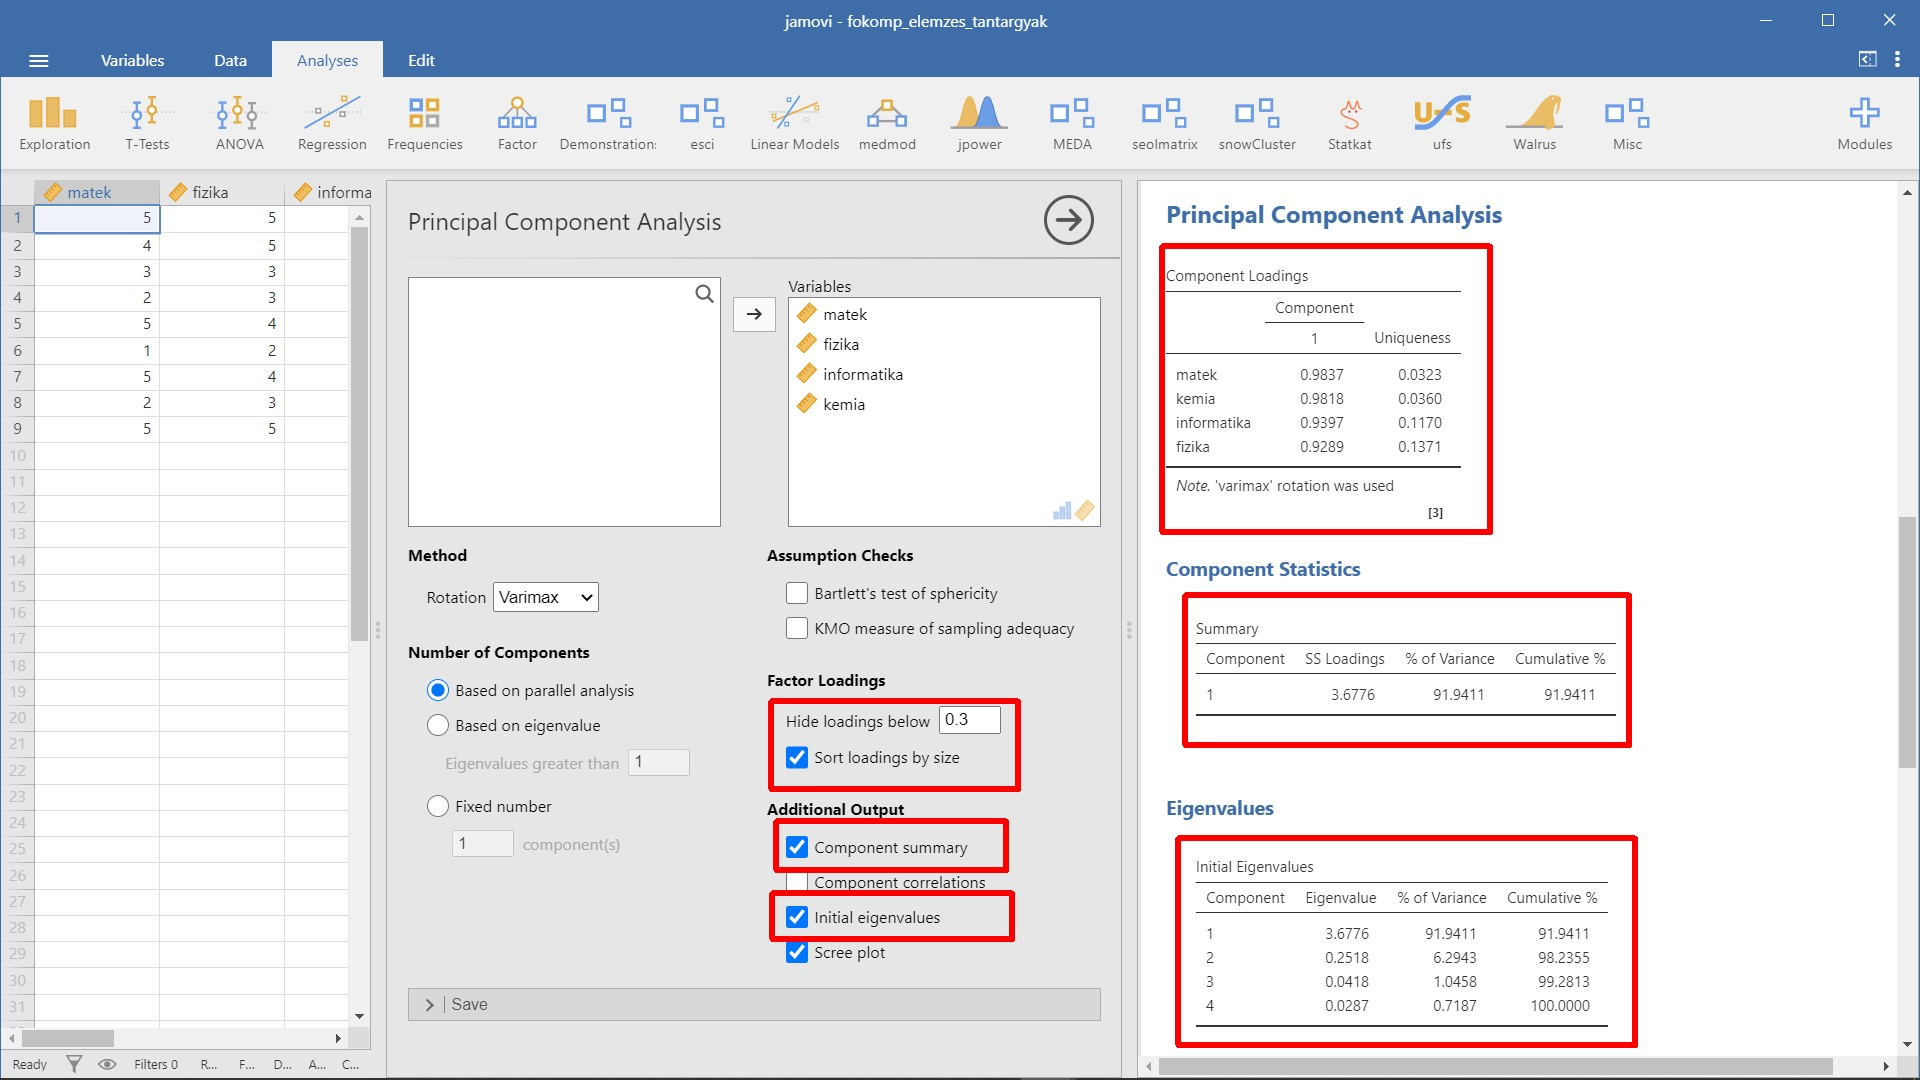
\includegraphics{./images/fokomponens_kep_04.jpg}

}

\caption{Komponensek összegzése}

\end{figure}

\textbf{6. Főkomponens értékek kiszámítása}

A főkomponens elemzés célja az eredeti változók csökkentése. A
főkomponens(ek) az eredeti változók lineáris kombinációjával
kifejezhetők. Ez(ek) a főkomponens értékek (jamovi-ban:
\texttt{Component\ score}) az adatbázisban is rögzíthetők, és további
elemzések kiindulópontjai lehetnek.

\begin{figure}

{\centering 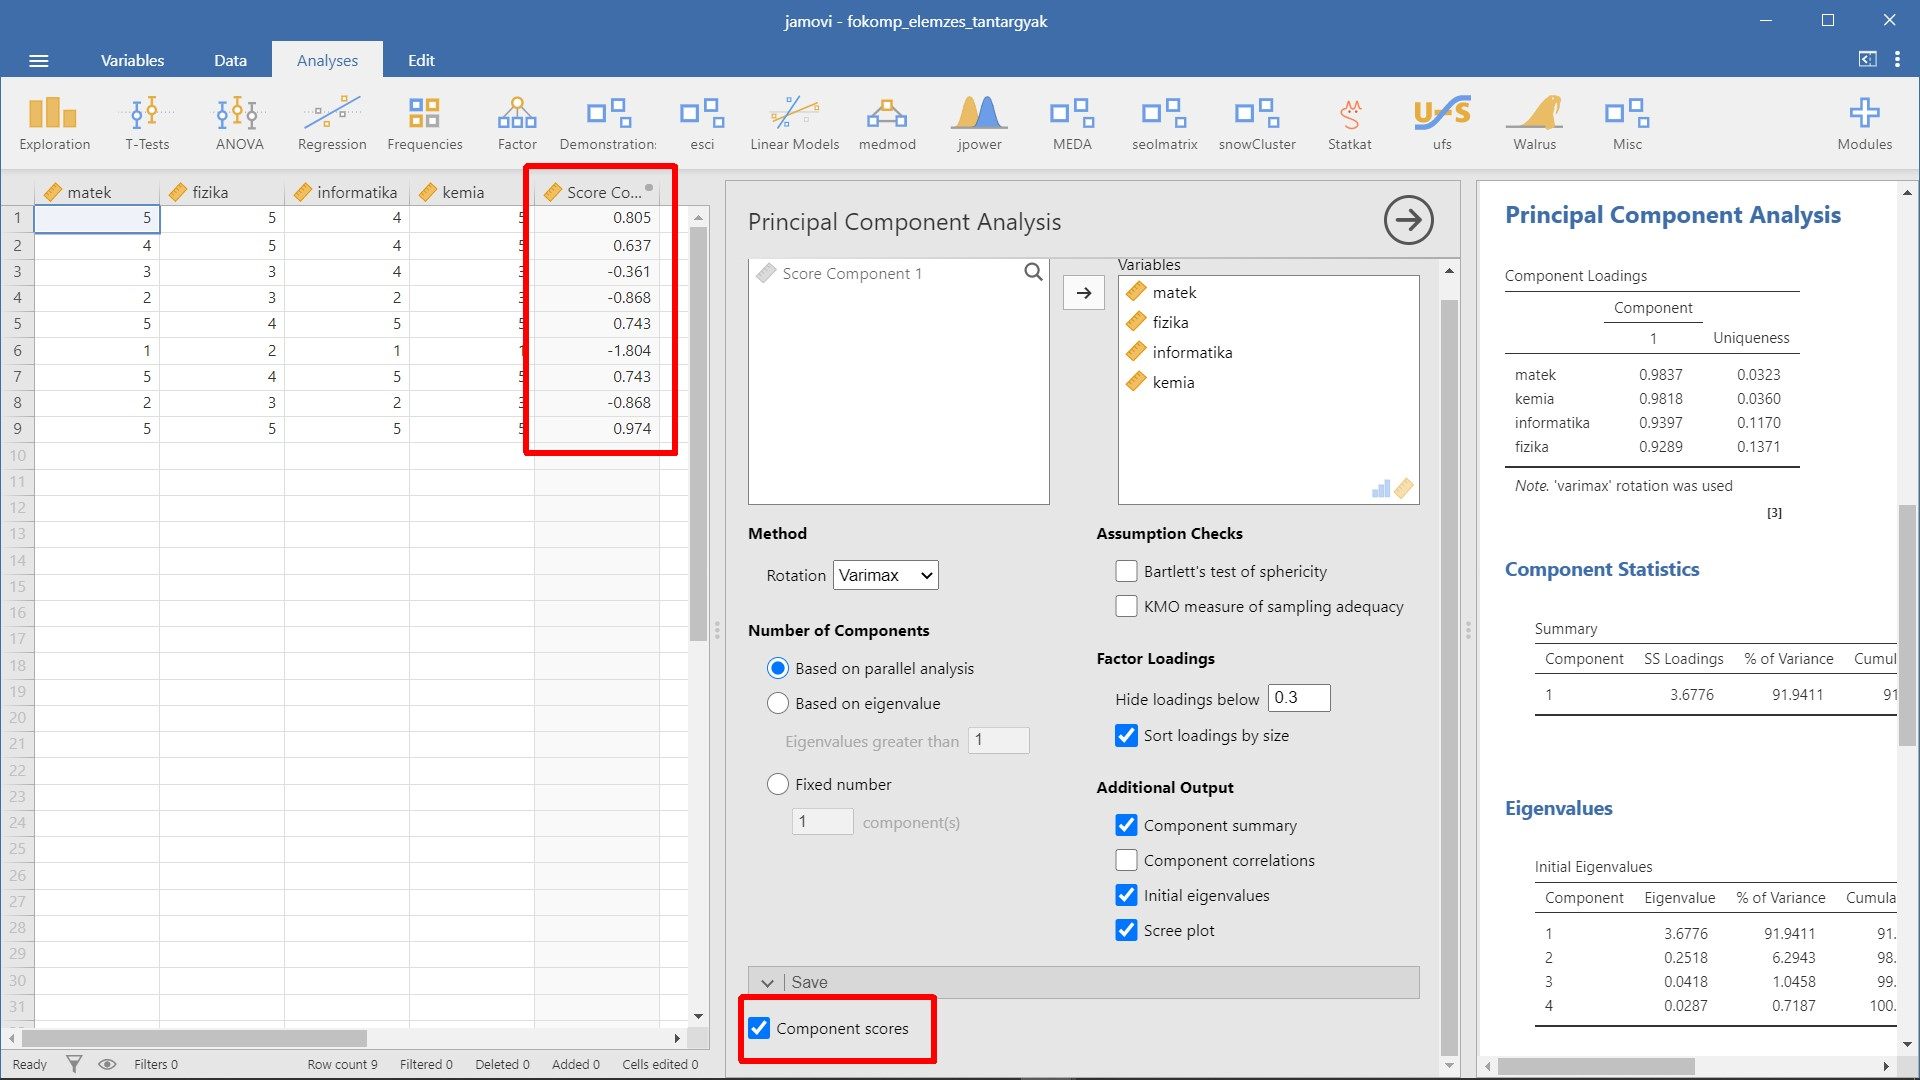
\includegraphics{./images/fokomponens_kep_05.jpg}

}

\caption{Főkomponens értékek kiszámítása}

\end{figure}

Sikerült tehát az érdemjegyeket egyetlen mérőszámmal kifejezni, a fenti
főkomponens érték az, amely a lehető legjobban magában foglalja az egyes
tantárgyakból szerzett jegyeket és ezáltal a reál tantárgyak iránti
fogékonyság mérőszáma lehet. A legjobban a kilencedik személy teljesít a
reál tárgyakból, legrosszabbul pedig a hatodik. Ezek az értékek
standardizáltak, vagyis 0 átlagúak és 1 szórásúak.

\begin{figure}

{\centering 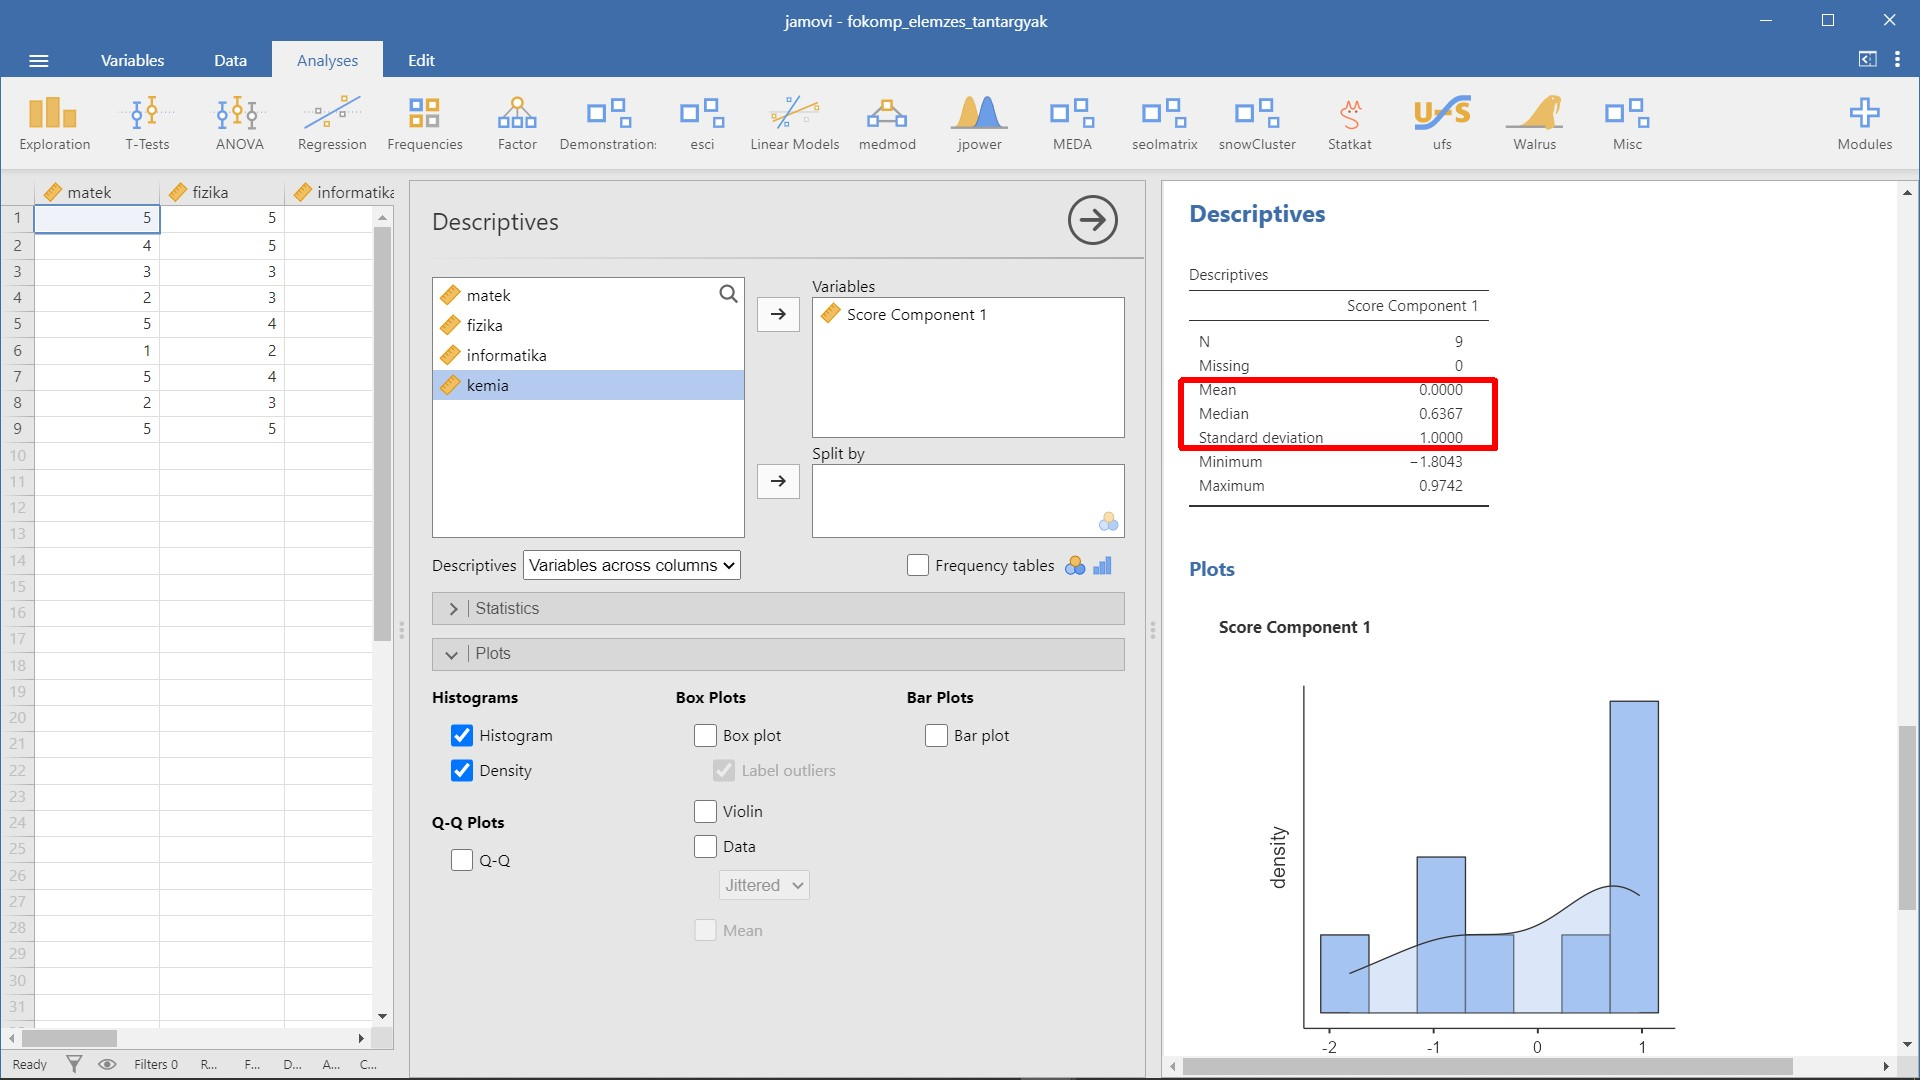
\includegraphics{./images/fokomponens_kep_06.jpg}

}

\caption{Főkomponens értékek leíró statisztikája}

\end{figure}

R-ben több lehetőségünk van a főlomponenselemzés elvégzésére.

\begin{Shaded}
\begin{Highlighting}[]
\NormalTok{pca\_1 }\OtherTok{\textless{}{-}} \FunctionTok{prcomp}\NormalTok{(d, }\AttributeTok{scale. =} \ConstantTok{TRUE}\NormalTok{)}
\NormalTok{pca\_1}
\CommentTok{\#\textgreater{} Standard deviations (1, .., p=4):}
\CommentTok{\#\textgreater{} [1] 1.9177188 0.5017701 0.2045278 0.1695572}
\CommentTok{\#\textgreater{} }
\CommentTok{\#\textgreater{} Rotation (n x k) = (4 x 4):}
\CommentTok{\#\textgreater{}                    PC1        PC2         PC3}
\CommentTok{\#\textgreater{} matek       {-}0.5129614  0.2231620 {-}0.02972158}
\CommentTok{\#\textgreater{} fizika      {-}0.4843985 {-}0.7077528  0.50610146}
\CommentTok{\#\textgreater{} informatika {-}0.4900124  0.6474152  0.35260295}
\CommentTok{\#\textgreater{} kemia       {-}0.5119731 {-}0.1736040 {-}0.78654250}
\CommentTok{\#\textgreater{}                     PC4}
\CommentTok{\#\textgreater{} matek       {-}0.82836339}
\CommentTok{\#\textgreater{} fizika       0.09113404}
\CommentTok{\#\textgreater{} informatika  0.46520167}
\CommentTok{\#\textgreater{} kemia        0.29848968}
\end{Highlighting}
\end{Shaded}

\begin{Shaded}
\begin{Highlighting}[]
\NormalTok{pca\_1 }\OtherTok{\textless{}{-}} \FunctionTok{princomp}\NormalTok{(d, }\AttributeTok{cor =} \ConstantTok{TRUE}\NormalTok{)}
\NormalTok{pca\_1}
\CommentTok{\#\textgreater{} Call:}
\CommentTok{\#\textgreater{} princomp(x = d, cor = TRUE)}
\CommentTok{\#\textgreater{} }
\CommentTok{\#\textgreater{} Standard deviations:}
\CommentTok{\#\textgreater{}    Comp.1    Comp.2    Comp.3    Comp.4 }
\CommentTok{\#\textgreater{} 1.9177188 0.5017701 0.2045278 0.1695572 }
\CommentTok{\#\textgreater{} }
\CommentTok{\#\textgreater{}  4  variables and  9 observations.}
\end{Highlighting}
\end{Shaded}

\begin{Shaded}
\begin{Highlighting}[]
\NormalTok{psych}\SpecialCharTok{::}\FunctionTok{pca}\NormalTok{(d, }\AttributeTok{rotate =} \StringTok{"varimax"}\NormalTok{)}
\CommentTok{\#\textgreater{} Principal Components Analysis}
\CommentTok{\#\textgreater{} Call: principal(r = r, nfactors = nfactors, residua...}
\CommentTok{\#\textgreater{}     rotate = rotate, n.obs = n.obs, covar = covar, ...}
\CommentTok{\#\textgreater{}     missing = missing, impute = impute, oblique.sco...}
\CommentTok{\#\textgreater{}     method = method, use = use, cor = cor, correct ...}
\CommentTok{\#\textgreater{} Standardized loadings (pattern matrix) based upon c...}
\CommentTok{\#\textgreater{}              PC1   h2    u2 com}
\CommentTok{\#\textgreater{} matek       0.98 0.97 0.032   1}
\CommentTok{\#\textgreater{} fizika      0.93 0.86 0.137   1}
\CommentTok{\#\textgreater{} informatika 0.94 0.88 0.117   1}
\CommentTok{\#\textgreater{} kemia       0.98 0.96 0.036   1}
\CommentTok{\#\textgreater{} }
\CommentTok{\#\textgreater{}                 PC1}
\CommentTok{\#\textgreater{} SS loadings    3.68}
\CommentTok{\#\textgreater{} Proportion Var 0.92}
\CommentTok{\#\textgreater{} }
\CommentTok{\#\textgreater{} Mean item complexity =  1}
\CommentTok{\#\textgreater{} Test of the hypothesis that 1 component is sufficient.}
\CommentTok{\#\textgreater{} }
\CommentTok{\#\textgreater{} The root mean square of the residuals (RMSR) is  0.05 }
\CommentTok{\#\textgreater{}  with the empirical chi square  0.28  with prob \textless{}  ...}
\CommentTok{\#\textgreater{} }
\CommentTok{\#\textgreater{} Fit based upon off diagonal values = 1}
\end{Highlighting}
\end{Shaded}

\begin{Shaded}
\begin{Highlighting}[]
\NormalTok{pca\_1 }\OtherTok{\textless{}{-}}\NormalTok{ FactoMineR}\SpecialCharTok{::}\FunctionTok{PCA}\NormalTok{(d, }\AttributeTok{graph =} \ConstantTok{FALSE}\NormalTok{)}
\NormalTok{pca\_1}\SpecialCharTok{$}\NormalTok{eig}
\CommentTok{\#\textgreater{}        eigenvalue percentage of variance}
\CommentTok{\#\textgreater{} comp 1 3.67764553             91.9411383}
\CommentTok{\#\textgreater{} comp 2 0.25177321              6.2943303}
\CommentTok{\#\textgreater{} comp 3 0.04183160              1.0457901}
\CommentTok{\#\textgreater{} comp 4 0.02874965              0.7187414}
\CommentTok{\#\textgreater{}        cumulative percentage of variance}
\CommentTok{\#\textgreater{} comp 1                          91.94114}
\CommentTok{\#\textgreater{} comp 2                          98.23547}
\CommentTok{\#\textgreater{} comp 3                          99.28126}
\CommentTok{\#\textgreater{} comp 4                         100.00000}
\NormalTok{pca\_1}\SpecialCharTok{$}\NormalTok{var}
\CommentTok{\#\textgreater{} $coord}
\CommentTok{\#\textgreater{}                 Dim.1      Dim.2        Dim.3}
\CommentTok{\#\textgreater{} matek       0.9837158 {-}0.1119760 {-}0.006078888}
\CommentTok{\#\textgreater{} fizika      0.9289402  0.3551292  0.103511795}
\CommentTok{\#\textgreater{} informatika 0.9397061 {-}0.3248536  0.072117091}
\CommentTok{\#\textgreater{} kemia       0.9818205  0.0871093 {-}0.160869772}
\CommentTok{\#\textgreater{}                   Dim.4}
\CommentTok{\#\textgreater{} matek       {-}0.14045500}
\CommentTok{\#\textgreater{} fizika       0.01545243}
\CommentTok{\#\textgreater{} informatika  0.07887831}
\CommentTok{\#\textgreater{} kemia        0.05061108}
\CommentTok{\#\textgreater{} }
\CommentTok{\#\textgreater{} $cor}
\CommentTok{\#\textgreater{}                 Dim.1      Dim.2        Dim.3}
\CommentTok{\#\textgreater{} matek       0.9837158 {-}0.1119760 {-}0.006078888}
\CommentTok{\#\textgreater{} fizika      0.9289402  0.3551292  0.103511795}
\CommentTok{\#\textgreater{} informatika 0.9397061 {-}0.3248536  0.072117091}
\CommentTok{\#\textgreater{} kemia       0.9818205  0.0871093 {-}0.160869772}
\CommentTok{\#\textgreater{}                   Dim.4}
\CommentTok{\#\textgreater{} matek       {-}0.14045500}
\CommentTok{\#\textgreater{} fizika       0.01545243}
\CommentTok{\#\textgreater{} informatika  0.07887831}
\CommentTok{\#\textgreater{} kemia        0.05061108}
\CommentTok{\#\textgreater{} }
\CommentTok{\#\textgreater{} $cos2}
\CommentTok{\#\textgreater{}                 Dim.1       Dim.2        Dim.3}
\CommentTok{\#\textgreater{} matek       0.9676968 0.012538628 3.695288e{-}05}
\CommentTok{\#\textgreater{} fizika      0.8629298 0.126116721 1.071469e{-}02}
\CommentTok{\#\textgreater{} informatika 0.8830475 0.105529830 5.200875e{-}03}
\CommentTok{\#\textgreater{} kemia       0.9639714 0.007588031 2.587908e{-}02}
\CommentTok{\#\textgreater{}                    Dim.4}
\CommentTok{\#\textgreater{} matek       0.0197276074}
\CommentTok{\#\textgreater{} fizika      0.0002387777}
\CommentTok{\#\textgreater{} informatika 0.0062217871}
\CommentTok{\#\textgreater{} kemia       0.0025614817}
\CommentTok{\#\textgreater{} }
\CommentTok{\#\textgreater{} $contrib}
\CommentTok{\#\textgreater{}                Dim.1     Dim.2       Dim.3      Dim.4}
\CommentTok{\#\textgreater{} matek       26.31294  4.980128  0.08833723 68.6185908}
\CommentTok{\#\textgreater{} fizika      23.46419 50.091398 25.61386842  0.8305413}
\CommentTok{\#\textgreater{} informatika 24.01122 41.914638 12.43288421 21.6412590}
\CommentTok{\#\textgreater{} kemia       26.21165  3.013836 61.86491013  8.9096089}
\NormalTok{factoextra}\SpecialCharTok{::}\FunctionTok{fviz\_eig}\NormalTok{(pca\_1, }\AttributeTok{addlabels =} \ConstantTok{TRUE}\NormalTok{, }\AttributeTok{ylim =} \FunctionTok{c}\NormalTok{(}\DecValTok{0}\NormalTok{, }\DecValTok{110}\NormalTok{))}
\NormalTok{factoextra}\SpecialCharTok{::}\FunctionTok{get\_eigenvalue}\NormalTok{(pca\_1)}
\CommentTok{\#\textgreater{}       eigenvalue variance.percent}
\CommentTok{\#\textgreater{} Dim.1 3.67764553       91.9411383}
\CommentTok{\#\textgreater{} Dim.2 0.25177321        6.2943303}
\CommentTok{\#\textgreater{} Dim.3 0.04183160        1.0457901}
\CommentTok{\#\textgreater{} Dim.4 0.02874965        0.7187414}
\CommentTok{\#\textgreater{}       cumulative.variance.percent}
\CommentTok{\#\textgreater{} Dim.1                    91.94114}
\CommentTok{\#\textgreater{} Dim.2                    98.23547}
\CommentTok{\#\textgreater{} Dim.3                    99.28126}
\CommentTok{\#\textgreater{} Dim.4                   100.00000}
\NormalTok{factoextra}\SpecialCharTok{::}\FunctionTok{get\_pca\_ind}\NormalTok{(pca\_1)}
\CommentTok{\#\textgreater{} Principal Component Analysis Results for individuals}
\CommentTok{\#\textgreater{}  ===================================================}
\CommentTok{\#\textgreater{}   Name       Description                       }
\CommentTok{\#\textgreater{} 1 "$coord"   "Coordinates for the individuals" }
\CommentTok{\#\textgreater{} 2 "$cos2"    "Cos2 for the individuals"        }
\CommentTok{\#\textgreater{} 3 "$contrib" "contributions of the individuals"}
\NormalTok{factoextra}\SpecialCharTok{::}\FunctionTok{get\_pca\_var}\NormalTok{(pca\_1)}
\CommentTok{\#\textgreater{} Principal Component Analysis Results for variables}
\CommentTok{\#\textgreater{}  ===================================================}
\CommentTok{\#\textgreater{}   Name      }
\CommentTok{\#\textgreater{} 1 "$coord"  }
\CommentTok{\#\textgreater{} 2 "$cor"    }
\CommentTok{\#\textgreater{} 3 "$cos2"   }
\CommentTok{\#\textgreater{} 4 "$contrib"}
\CommentTok{\#\textgreater{}   Description                                    }
\CommentTok{\#\textgreater{} 1 "Coordinates for the variables"                }
\CommentTok{\#\textgreater{} 2 "Correlations between variables and dimensions"}
\CommentTok{\#\textgreater{} 3 "Cos2 for the variables"                       }
\CommentTok{\#\textgreater{} 4 "contributions of the variables"}
\NormalTok{factoextra}\SpecialCharTok{::}\FunctionTok{fviz\_pca\_ind}\NormalTok{(pca\_1)}
\NormalTok{factoextra}\SpecialCharTok{::}\FunctionTok{fviz\_pca\_var}\NormalTok{(pca\_1)}
\NormalTok{factoextra}\SpecialCharTok{::}\FunctionTok{fviz\_pca\_biplot}\NormalTok{(pca\_1)}
\NormalTok{corrplot}\SpecialCharTok{::}\FunctionTok{corrplot}\NormalTok{(pca\_1}\SpecialCharTok{$}\NormalTok{var}\SpecialCharTok{$}\NormalTok{cos2, }\AttributeTok{is.corr =} \ConstantTok{FALSE}\NormalTok{)}
\end{Highlighting}
\end{Shaded}

\begin{figure}[H]

{\centering 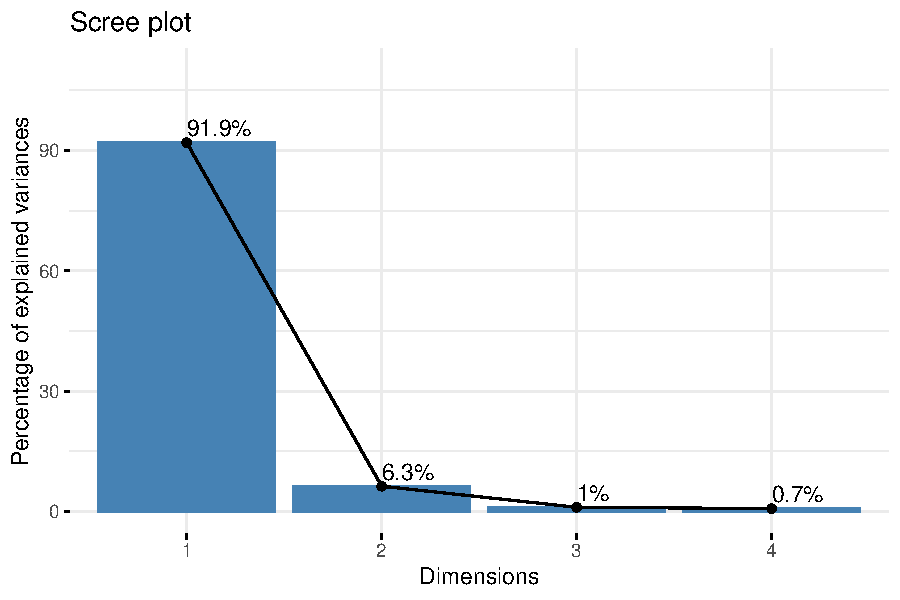
\includegraphics{./sec_fokomponens_elemzes_files/figure-pdf/unnamed-chunk-7-1.pdf}

}

\end{figure}

\begin{figure}[H]

{\centering 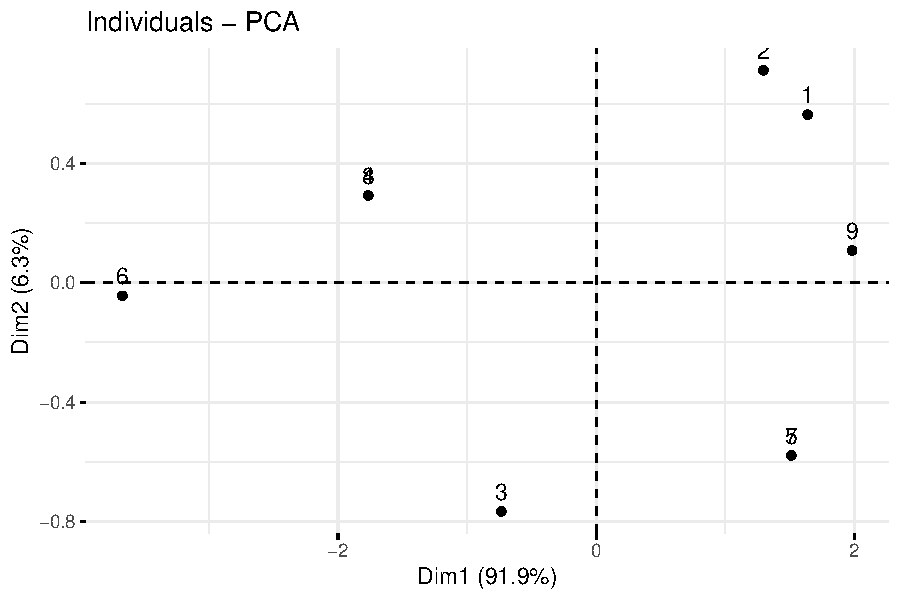
\includegraphics{./sec_fokomponens_elemzes_files/figure-pdf/unnamed-chunk-7-2.pdf}

}

\end{figure}

\begin{figure}[H]

{\centering 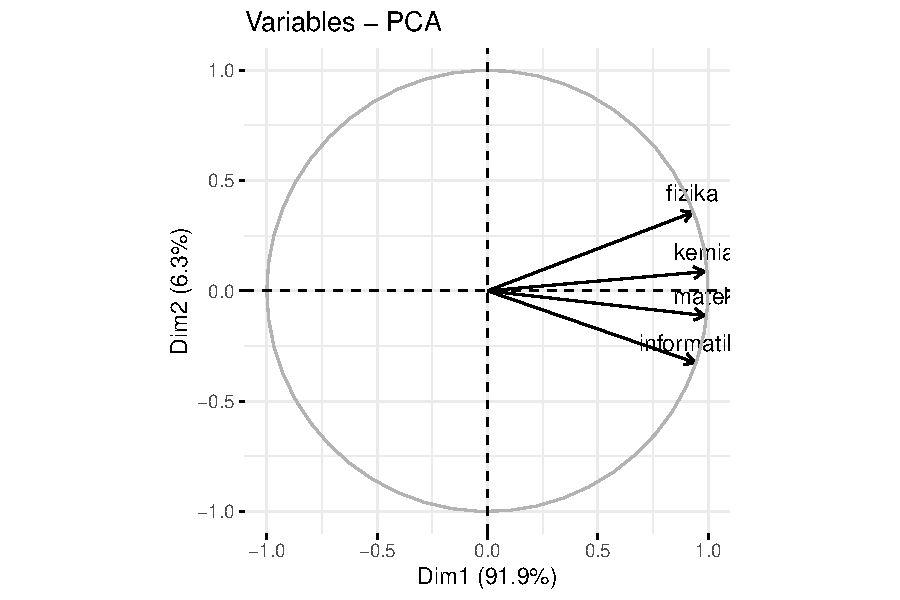
\includegraphics{./sec_fokomponens_elemzes_files/figure-pdf/unnamed-chunk-7-3.pdf}

}

\end{figure}

\begin{figure}[H]

{\centering 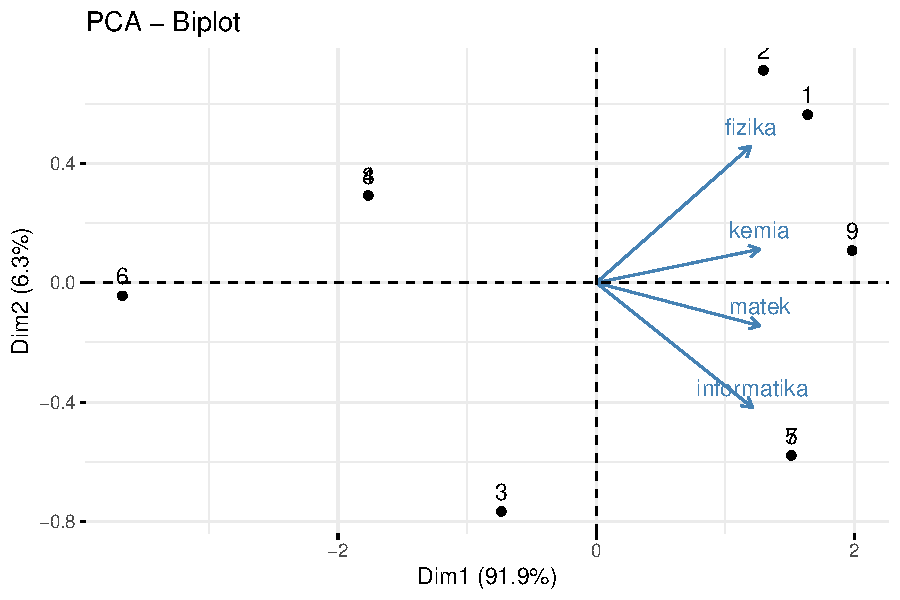
\includegraphics{./sec_fokomponens_elemzes_files/figure-pdf/unnamed-chunk-7-4.pdf}

}

\end{figure}

\begin{figure}[H]

{\centering 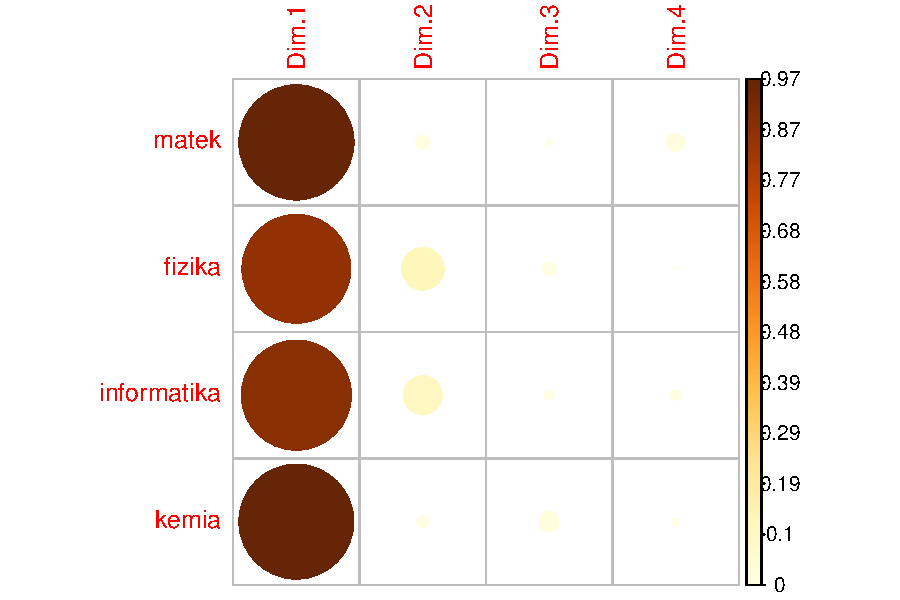
\includegraphics{./sec_fokomponens_elemzes_files/figure-pdf/unnamed-chunk-7-5.pdf}

}

\end{figure}

\begin{enumerate}
\def\labelenumi{\arabic{enumi}.}
\setcounter{enumi}{1}
\tightlist
\item
  Példa
\end{enumerate}

Létezik a reál tárgyak iránti fogékonyság?

Korábban már foglalkoztunk azzal a felvetéssel, hogy néhány tantárgy
eredményeit egyetlen mérőszámmal reprezentáljuk. Korábbi példánkban a
matematika, fizika, informatika és kémia jegyek közötti összefüggéseket
vizsgáltuk egy kisebb adatbázison, most egy sokkal nagyobb adatbázis
segítségével mutatjuk be, hogyan végezhetünk főkomponens-analízist.

Összességében az adatok jól sűríthetők egyetlen mérőszámba, minimális
információveszteséggel, ezt a mutatót pedig hívhatjuk a reál tárgyak
iránti fogékonyság mutatójának.

\begin{enumerate}
\def\labelenumi{\arabic{enumi}.}
\setcounter{enumi}{2}
\tightlist
\item
  Példa
\end{enumerate}

Egy kérdőív szerkesztésének problémái

A kapott eredmények alapján az itemszelekciót ennél a lépésnél
befejezhetjük. Az így kapott hat itemünk a statisztikai eredmények
alapján egészen jól lefednek egy dimenziót, ezáltal használhatóak egy
jelenség kérdőíves vizsgálatára.

\bookmarksetup{startatroot}

\hypertarget{sec-megbizhatosag-elemzes}{%
\chapter{Megbízhatóság elemzés}\label{sec-megbizhatosag-elemzes}}

A pszichológiai tesztelés során használt mérőeszközök legfontosabb
tulajdonsága a megbízhatóság (reliabilitás) és a validitás (Carver és
Scheier, 2006; Nagy, 2006). A reliabilitás azt mutatja meg, hogy az
eszköz mennyire mér megbízhatóan, pontosan, mennyire bízhatunk abban,
hogy a mérés második és harmadik alkalommal is ugyanazt az eredményt
adja, amit az első esetben. A validitás vagy érvényesség azt jelenti,
hogy a mérőeszköz azt méri, amit mérni szeretnénk. A klasszikus
ábrázolás szerint mérőeszközünk a megbízhatóság és az érvényesség
alapján a lenti négy csoportok egyikébe is eshet:

\begin{figure}

{\centering 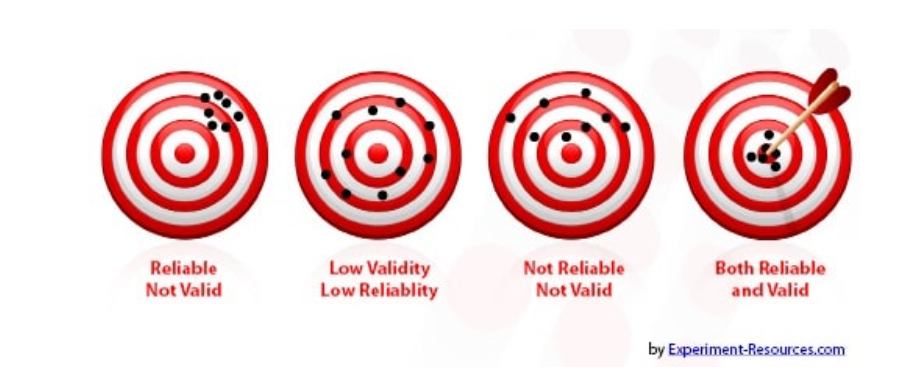
\includegraphics{./images/megbizhatosag_kep_01.png}

}

\caption{Megbízhatóság és validitás esetei}

\end{figure}

Egy mérőeszköz megbízhatóságát mindig úgy vizsgáljuk, hogy a mérés
eredményét egy vagy több más eszköz eredményével hasonlítjuk össze. Az
összehasonlítás mindig korrelációt típusú vizsgálatot jelent, és a
magasabb korreláció egyben magasabb megbízhatóságot jelöl. Ennek
megfelelően a megbízhatósági mutatók értéktartománya megegyezik a
korrelációs együttható értéktartományával (feltehetően azonban 0 és 1
közötti lesz az értéke, negatív értéket ritkán kapunk és el is
szeretnénk kerülni).

A megbízhatósággal kapcsolatban három aspektust érdemes vizsgálni:

\begin{itemize}
\tightlist
\item
  \textbf{belső konzisztencia} -- az önjellemző skálák sok tételből
  állnak (melyik mindegyike külön mérőeszköznek tekinthető), ezek
  kitöltésével egyidejűleg végzünk egymással ekvivalens, párhuzamos
  méréseket.
\item
  \textbf{időbeli stabiltás (teszt-reteszt reliabilitás)} -- időben
  eltolva, ugyanazon mérést egy későbbi időpontban megismételve jutunk
  két mérési eredményhez, például, ha ugyanazt az önjellemző skálát
  mondjuk, egy nap eltéréssel felvesszük ugyanazon személyekkel.
\item
  \textbf{értékelő megbízhatóság (inter-rater reliabilitás)} -- amikor
  megfigyelő pontoz, akkor a megfigyelő személy a mérőeszköz, így a
  megfigyelői ítéleteket az értékelő megbízhatóságának meghatározásával
  ellenőrizzük.
\end{itemize}

\hypertarget{cronbach-alfa-belsux151-konzisztencia-muxe9ruxe9se}{%
\section{Cronbach-alfa -- belső konzisztencia
mérése}\label{cronbach-alfa-belsux151-konzisztencia-muxe9ruxe9se}}

Főkomponens elemzés segítségével könnyen tudunk több változót -
viszonylag csekély veszteséggel - egyetlen változóba tömöríteni, ezért
gyakran használják kérdőívek itemeinek szelekciójára, valamint
megbízhatóság (reliabilitás) vizsgálatra. A klasszikus tesztelmélet
keretein belül azonban a tesztek megbízhatóságának (reliabilitásának)
több lehetséges mutatója is létezik.

Cronbach 1951-es munkájában publikálta azon nézetét, hogy a korábbi
egyszerű tesztfelezéses eljárás helyett egy annál tökéletesebb mutatót
kellene használni a tesztek megbízhatóságának indikátoraként. Ha az
itemek száma alacsony vagy az itemek közötti átlagos korreláció
alacsony, akkor csökkenni fog a Cronbach-féle alfa értéke is. Az is
egyértelmű, hogy az itemek közötti alacsony korreláció arra enged
következtetni, hogy a teszt itemjei nem egy és ugyanazon dolog
vizsgálatára szolgálnak, a belőlük képzendő tesztérték nem alkalmas sem
elméleti, sem pedig gyakorlati felhasználásra.

Az ómega (McDonald \(\omega\)) korrigálja a Cronbach-alfa torzítását,
érdemes elvégezni az elemzést ezzel a mutatóval is (Kárász és mtsai.,
2022; Malkewitz és mtsai., 2023).

\hypertarget{puxe9lda-real-tuxe1rgyak-iruxe1nti-foguxe9konysuxe1g}{%
\section{Példa: Real tárgyak iránti
fogékonyság}\label{puxe9lda-real-tuxe1rgyak-iruxe1nti-foguxe9konysuxe1g}}

Egy fiktív adatbázis 9 tanuló iskolai jegyeit tartalamzza reál
tantárgyakból (matematika, fizika, kémia, informatika)
(\texttt{megbizhatosag\_tantargyak.xlsx}). Vizsgáljuk meg, ha a reál
tantárgyak iránti fogékonyságot ezzel a 4 érdemjeggyel mérnénk, akkor ez
megbízhatóság szempontjából alkalmas mérőeszköz lenne.

\begin{Shaded}
\begin{Highlighting}[]
\NormalTok{real }\OtherTok{\textless{}{-}}\NormalTok{ rio}\SpecialCharTok{::}\FunctionTok{import}\NormalTok{(}\AttributeTok{file =} \StringTok{"adat/megbizhatosag\_tantargyak.xlsx"}\NormalTok{)}
\FunctionTok{str}\NormalTok{(real)}
\CommentTok{\#\textgreater{} \textquotesingle{}data.frame\textquotesingle{}:    9 obs. of  4 variables:}
\CommentTok{\#\textgreater{}  $ matek      : num  5 4 3 2 5 1 5 2 5}
\CommentTok{\#\textgreater{}  $ fizika     : num  5 5 3 3 4 2 4 3 5}
\CommentTok{\#\textgreater{}  $ informatika: num  4 4 4 2 5 1 5 2 5}
\CommentTok{\#\textgreater{}  $ kemia      : num  5 5 3 3 5 1 5 3 5}
\end{Highlighting}
\end{Shaded}

A Cronbach alfa meghatározását végezhetjük a \texttt{\{psych\}} csomag
\texttt{alpha()} függvényével.

\begin{Shaded}
\begin{Highlighting}[]
\NormalTok{psych}\SpecialCharTok{::}\FunctionTok{alpha}\NormalTok{(real)  }\CommentTok{\# Cronbach{-}alfa}
\CommentTok{\#\textgreater{} }
\CommentTok{\#\textgreater{} Reliability analysis   }
\CommentTok{\#\textgreater{} Call: psych::alpha(x = real)}
\CommentTok{\#\textgreater{} }
\CommentTok{\#\textgreater{}   raw\_alpha std.alpha G6(smc) average\_r S/N   ase mean}
\CommentTok{\#\textgreater{}       0.97      0.97    0.98      0.89  33 0.017  3.7}
\CommentTok{\#\textgreater{}   sd median\_r}
\CommentTok{\#\textgreater{}  1.4     0.91}
\CommentTok{\#\textgreater{} }
\CommentTok{\#\textgreater{}     95\% confidence boundaries }
\CommentTok{\#\textgreater{}          lower alpha upper}
\CommentTok{\#\textgreater{} Feldt     0.91  0.97  0.99}
\CommentTok{\#\textgreater{} Duhachek  0.93  0.97  1.00}
\CommentTok{\#\textgreater{} }
\CommentTok{\#\textgreater{}  Reliability if an item is dropped:}
\CommentTok{\#\textgreater{}             raw\_alpha std.alpha G6(smc) average\_r S/N}
\CommentTok{\#\textgreater{} matek            0.94      0.95    0.95      0.86  18}
\CommentTok{\#\textgreater{} fizika           0.97      0.98    0.97      0.93  39}
\CommentTok{\#\textgreater{} informatika      0.96      0.97    0.97      0.92  33}
\CommentTok{\#\textgreater{} kemia            0.94      0.95    0.96      0.86  19}
\CommentTok{\#\textgreater{}             alpha se  var.r med.r}
\CommentTok{\#\textgreater{} matek          0.032 0.0070  0.89}
\CommentTok{\#\textgreater{} fizika         0.015 0.0013  0.95}
\CommentTok{\#\textgreater{} informatika    0.019 0.0016  0.93}
\CommentTok{\#\textgreater{} kemia          0.029 0.0084  0.87}
\CommentTok{\#\textgreater{} }
\CommentTok{\#\textgreater{}  Item statistics }
\CommentTok{\#\textgreater{}             n raw.r std.r r.cor r.drop mean  sd}
\CommentTok{\#\textgreater{} matek       9  0.99  0.98  0.98   0.97  3.6 1.6}
\CommentTok{\#\textgreater{} fizika      9  0.92  0.93  0.91   0.88  3.8 1.1}
\CommentTok{\#\textgreater{} informatika 9  0.95  0.94  0.93   0.90  3.6 1.5}
\CommentTok{\#\textgreater{} kemia       9  0.98  0.98  0.98   0.96  3.9 1.5}
\CommentTok{\#\textgreater{} }
\CommentTok{\#\textgreater{} Non missing response frequency for each item}
\CommentTok{\#\textgreater{}                1    2    3    4    5 miss}
\CommentTok{\#\textgreater{} matek       0.11 0.22 0.11 0.11 0.44    0}
\CommentTok{\#\textgreater{} fizika      0.00 0.11 0.33 0.22 0.33    0}
\CommentTok{\#\textgreater{} informatika 0.11 0.22 0.00 0.33 0.33    0}
\CommentTok{\#\textgreater{} kemia       0.11 0.00 0.33 0.00 0.56    0}
\end{Highlighting}
\end{Shaded}

A McDonald \(\omega\) értékét kiszámolhatjuk a \texttt{\{psych\}} csomag
\texttt{omega()} függvényével.

\begin{Shaded}
\begin{Highlighting}[]
\NormalTok{psych}\SpecialCharTok{::}\FunctionTok{omega}\NormalTok{(real, }\AttributeTok{plot =}\NormalTok{ F)  }\CommentTok{\# McDonald{-}ómega}
\CommentTok{\#\textgreater{} Omega }
\CommentTok{\#\textgreater{} Call: omegah(m = m, nfactors = nfactors, fm = fm, k...}
\CommentTok{\#\textgreater{}     digits = digits, title = title, sl = sl, labels...}
\CommentTok{\#\textgreater{}     plot = plot, n.obs = n.obs, rotate = rotate, Ph...}
\CommentTok{\#\textgreater{}     covar = covar)}
\CommentTok{\#\textgreater{} Alpha:                 0.97 }
\CommentTok{\#\textgreater{} G.6:                   0.98 }
\CommentTok{\#\textgreater{} Omega Hierarchical:    0.95 }
\CommentTok{\#\textgreater{} Omega H asymptotic:    0.96 }
\CommentTok{\#\textgreater{} Omega Total            0.99 }
\CommentTok{\#\textgreater{} }
\CommentTok{\#\textgreater{} Schmid Leiman Factor loadings greater than  0.2 }
\CommentTok{\#\textgreater{}                g   F1*   F2*   F3*   h2   u2   p2}
\CommentTok{\#\textgreater{} matek       0.97        0.28       0.99 0.01 0.94}
\CommentTok{\#\textgreater{} fizika      0.89  0.29             0.92 0.08 0.86}
\CommentTok{\#\textgreater{} informatika 0.91        0.28       0.95 0.05 0.87}
\CommentTok{\#\textgreater{} kemia       0.96  0.29             0.99 0.01 0.94}
\CommentTok{\#\textgreater{} }
\CommentTok{\#\textgreater{} With Sums of squares  of:}
\CommentTok{\#\textgreater{}    g  F1*  F2*  F3* }
\CommentTok{\#\textgreater{} 3.48 0.17 0.16 0.04 }
\CommentTok{\#\textgreater{} }
\CommentTok{\#\textgreater{} general/max  21.07   max/min =   4.03}
\CommentTok{\#\textgreater{} mean percent general =  0.9    with sd =  0.04 and ...}
\CommentTok{\#\textgreater{} Explained Common Variance of the general factor =  ...}
\CommentTok{\#\textgreater{} }
\CommentTok{\#\textgreater{} The degrees of freedom are {-}3  and the fit is  0 }
\CommentTok{\#\textgreater{} The number of observations was  9  with Chi Square ...}
\CommentTok{\#\textgreater{} The root mean square of the residuals is  0 }
\CommentTok{\#\textgreater{} The df corrected root mean square of the residuals ...}
\CommentTok{\#\textgreater{} }
\CommentTok{\#\textgreater{} Compare this with the adequacy of just a general fa...}
\CommentTok{\#\textgreater{} The degrees of freedom for just the general factor ...}
\CommentTok{\#\textgreater{} The number of observations was  9  with Chi Square ...}
\CommentTok{\#\textgreater{} The root mean square of the residuals is  0.05 }
\CommentTok{\#\textgreater{} The df corrected root mean square of the residuals ...}
\CommentTok{\#\textgreater{} }
\CommentTok{\#\textgreater{} RMSEA index =  0.401  and the 10 \% confidence inter...}
\CommentTok{\#\textgreater{} BIC =  0.75 }
\CommentTok{\#\textgreater{} }
\CommentTok{\#\textgreater{} Measures of factor score adequacy             }
\CommentTok{\#\textgreater{}                                                  g ...}
\CommentTok{\#\textgreater{} Correlation of scores with factors            0.98 ...}
\CommentTok{\#\textgreater{} Multiple R square of scores with factors      0.95 ...}
\CommentTok{\#\textgreater{} Minimum correlation of factor score estimates 0.90 ...}
\CommentTok{\#\textgreater{}                                                F2* ...}
\CommentTok{\#\textgreater{} Correlation of scores with factors            0.86 ...}
\CommentTok{\#\textgreater{} Multiple R square of scores with factors      0.74 ...}
\CommentTok{\#\textgreater{} Minimum correlation of factor score estimates 0.48 ...}
\CommentTok{\#\textgreater{} }
\CommentTok{\#\textgreater{}  Total, General and Subset omega for each subset}
\CommentTok{\#\textgreater{}                                                  g ...}
\CommentTok{\#\textgreater{} Omega total for total scores and subscales    0.99 ...}
\CommentTok{\#\textgreater{} Omega general for total scores and subscales  0.95 ...}
\CommentTok{\#\textgreater{} Omega group for total scores and subscales    0.04 ...}
\CommentTok{\#\textgreater{}                                                F2* F3*}
\CommentTok{\#\textgreater{} Omega total for total scores and subscales    0.99  NA}
\CommentTok{\#\textgreater{} Omega general for total scores and subscales  0.91  NA}
\CommentTok{\#\textgreater{} Omega group for total scores and subscales    0.08  NA}
\end{Highlighting}
\end{Shaded}

A fenti elemzéseket jamovi-ban a
\texttt{Factor\ /\ Reliability\ Analysis} menüpont segítségével
végezhetjük el.

\begin{figure}

{\centering 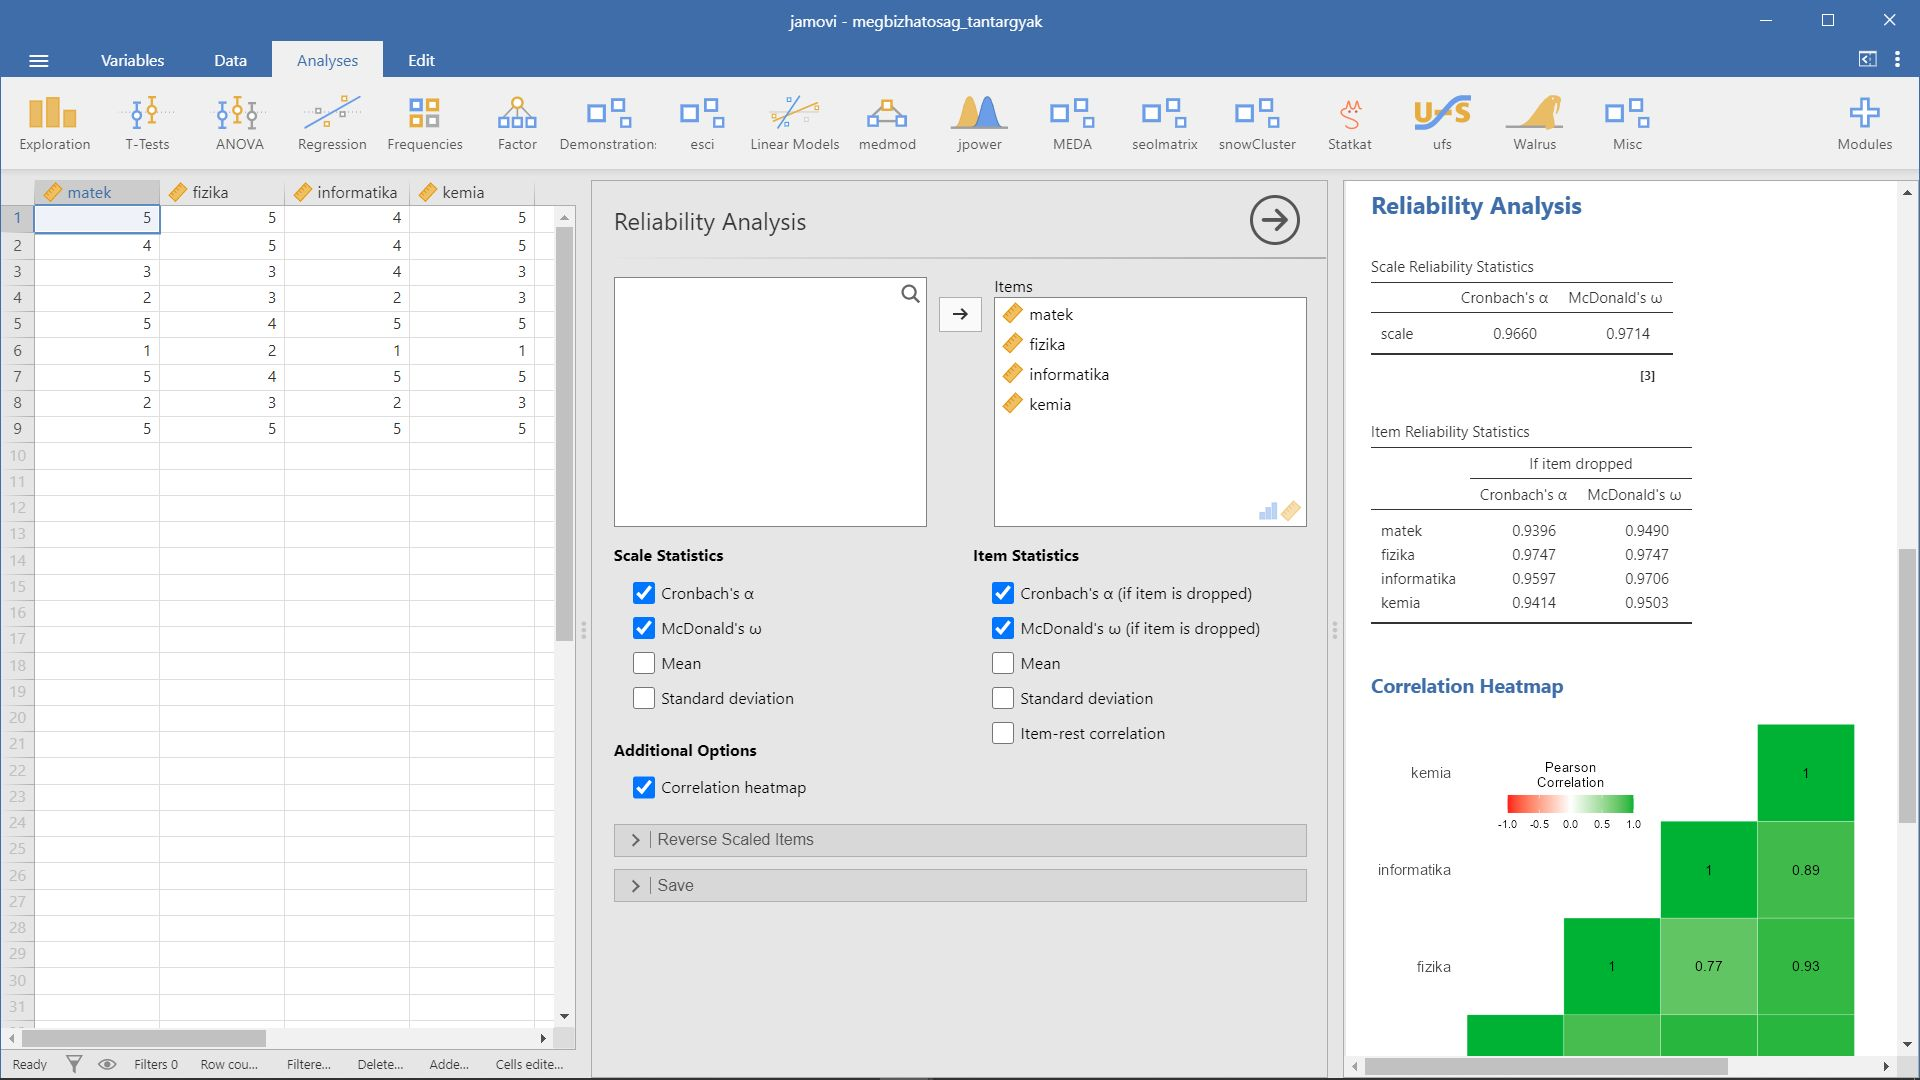
\includegraphics{./images/megbizhatosag_jamovi_kep_02.jpg}

}

\caption{Megbízhatóság elemzés jamovi-ban}

\end{figure}

A fenti megbízhatósági elemzések azt mutatják, hogy a négy tantárgy alfa
értéke 0,966, ami egy igen jó érték, hiszen közel van 1-hez (jamovi-ban:
Scale Reliability Statistics). Az Item Reliability Statistics táblázat
oszlopában szereplő értékek azt mutatják, mi történik, ha egy változót
kiveszünk a modellből. Láthatjuk, hogy egyedül a fizika változó értéke
növelné az alfát, de a növekedés mértéke elenyésző lenne, tehát nem éri
meg eltávolítani a változót, hiszen minél több információnk van egy
személyről, annál jobb.

\bookmarksetup{startatroot}

\hypertarget{sec-feltaro-faktorelemzes}{%
\chapter{Feltáró faktorelemzés}\label{sec-feltaro-faktorelemzes}}

A feltáró faktorelemzést új faktorok létrehozására használjuk, a
megerősítő faktorelemzést egy meglévő modell tesztelésére (lásd
következő fejezet). Ebben a fejezetben faktorelemzés alatt a feltáró
faktorelemzést értjük (Rózsa és mtsai., 2019; Watkins, 2018).

A lineáris regresszióelemzéstől eltérően a főkomponens- és a
faktorelemzés nagy számú változó kölcsönös összefüggésén alapuló
módszer, így nincsenek függő vagy független változóink. Elemzéskor a
változók korrelációs mátrixából indulunk ki.

\hypertarget{a-fux151komponens-elemzuxe9s-uxe9s-a-faktorelemzuxe9s-uxf6sszehasonluxedtuxe1sa}{%
\section{A főkomponens elemzés és a faktorelemzés
összehasonlítása}\label{a-fux151komponens-elemzuxe9s-uxe9s-a-faktorelemzuxe9s-uxf6sszehasonluxedtuxe1sa}}

\begin{itemize}
\tightlist
\item
  A főkomponens elemzés során az adatok teljes varianciáját vesszük
  figyelembe, míg faktorelemzés során a faktorokat csak a közös
  variancia alapján becsüljük. A két eljárás egyébként nagyon hasonló
  elvekre épül.

  \begin{itemize}
  \tightlist
  \item
    Főkomponens elemzés során a korrelációs mátrix átlójában lévő 1-esek
    összege adja teljes varianciát, ami teljes egészében bekerül a
    faktormodellbe. Ezért ez az eljárás akkor javasolt, ha a fő cél,
    hogy meghatározzuk azon főkomponensek (faktorok) legkisebb számát,
    amelyek a legtöbb varianciát magyarázzák. Ezek a faktorok később jól
    alkalmazhatók többváltozós elemzésekben. Összegezve: a főkomponens
    elemzésnél részinformációkat próbálunk összegezni a lehető legkisebb
    információveszteséggel (vagyis a variancia maximalizálásával).
  \item
    Az ún. közös faktorelemzésnél a faktorokat csak a közös variancia
    alapján becsüljük, vagyis a kommunalitások kerülnek a korrelációs
    mátrix átlójába (ezek 1-nél kisebb számok). Összegezve a
    faktorelemzés általános célja egy látens, lineáris struktúra
    feltárása manifeszt változók segítségével.
  \end{itemize}
\end{itemize}

\hypertarget{fogalmak}{%
\section{Fogalmak}\label{fogalmak}}

A főkomponens- és fakorelemzésben a következő fogalmak fordulnak elő (a
komponens és a faktor szavak felcserélhetők, attól függően, hogy
főkomponens- vagy fakorelemzésről van szó).

\begin{itemize}
\tightlist
\item
  \textbf{Kommuninalitás:} a variancia azon hányada, amelyen egy változó
  osztozik a többi elemzésbe vont változóval. Ez egyben a közös faktorok
  által magyarázott variancia aránya.
\item
  \textbf{Sajátérték:} Az egyes faktorok által magyarázott teljes
  varianciát fejezi ki.
\item
  \textbf{Faktorsúly:} A változók és a faktorok közötti közönséges
  korreláció.
\item
  \textbf{Faktormátrix:} Valamennyi változónak az összes előállított
  faktorra vonatkozó faktorsúlyát tartalmazza.
\item
  \textbf{Faktorértékek:} Az előállított faktoroknak az egyes
  megkérdezettekre vonatkozóan becsült értékei.
\item
  \textbf{Sajátértékábra (scree-plot, kőtörmelék ábra):} A sajátértékek
  ábrázolása az előállított faktorok sorszámának függvényében.
\item
  \textbf{Varianciahányad:} A teljes variancia egy adott faktornak
  tulajdonított része százalékban kifejezve.
\end{itemize}

\hypertarget{a-faktormodell}{%
\section{A faktormodell}\label{a-faktormodell}}

A főkomponens és faktorelemzés annyiban hasonlít a többszörös
regressziószámításhoz, hogy minden változót kifejezhető a háttérben
meghúzódó faktorok lineáris kombinációjaként. Minden egyes változó
kifejezhető kisszámú közös faktor és egy egyedi faktor segítségével.
Ezek a faktorok nem figyelhetők meg közvetlenül. Standardizált kiinduló
változók esetén a faktormodell így írható fel:

\begin{itemize}
\item
  \(X_i=A_{i1} F_1+A_{i2} F_2+\dots+ A_{im} F_m+V_i U_i\), ahol

  \begin{itemize}
  \tightlist
  \item
    \(X_i\) az \(i.\) standardizált változó
  \item
    \(A_{i1}\) az \(i.\) változó \(j.\) közös faktorra vonatkozó
    többszörös standardizált parciális regressziós együtthatója
  \item
    \(F_j\) a \(j.\) közös faktor
  \item
    \(V_i\) az \(i.\) változó \(j.\) egyedi faktorra vonatkozó
    többszörös standardizált parciális regressziós együtthatója
  \item
    \(U_i\) az \(i.\) változó egyedi faktora
  \item
    \(m\) a közös faktorok száma.
  \end{itemize}
\end{itemize}

Az egyedi faktorok egymással és a közös faktorokkal is korrelálatlanok.
A közös faktorok kifejezhetők a megfigyelt változók lineáris
kombinációiként:

\begin{itemize}
\tightlist
\item
  \(F_i=W_{i1} X_1+W_i2 X_2+\dots+ W_im X_m+\dots+ W_ik X_k\), ahol

  \begin{itemize}
  \tightlist
  \item
    \(F_i\) az \(i.\) faktor becslése
  \item
    \(W_i\) súly vagy a faktorérték együtthatója
  \item
    \(k\) a változók száma
  \end{itemize}
\end{itemize}

A súlyokat vagy faktorérték együtthatókat úgy is meg lehet választani,
hogy az első faktor magyarázza a teljes variancia legnagyobb részét, a
második faktor a második legnagyobb részét és így tovább, valamint, hogy
a faktorok korrelálatlanok legyenek egymással. Ez történik főkomponens
elemzés esetén.

\hypertarget{a-faktorelmzuxe9s-menete}{%
\section{A faktorelmzés menete}\label{a-faktorelmzuxe9s-menete}}

\textbf{1. A probléma megfogalmazása}

A kutató arra volt kíváncsi, milyen előnyöket keresnek a fogyasztók a
fogrémvásárlásnál. Egy 30 fős mintán a válaszadókat arra kérték, hogy
jelezzék, mennyire értenek egyet a következő állításokkal (1 =
egyáltalán nem ért egyet; 7 = teljes mértékben egyetért)

\begin{itemize}
\tightlist
\item
  v1: Fontos, hogy olyan fogkrémet vásároljak, amellyel megelőzhető a
  fogszuvasodás.
\item
  v2: Az olyan fogkrémeket szeretem, amely fényessé teszi a fogaimat.
\item
  v3: Egy fogkrémnek erősítenie kell a fogínyt.
\item
  v4: Az olyan fogkrémeket szeretem, amely friss leheletet biztosít.
\item
  v5: A fog romlásának megelőzése számomra nem fontos elvárás.
\item
  v6: A legfontosabb szempont a fogkrém vásárlásánál a szép fog.
\end{itemize}

\textbf{2. A korrelációs mátrix előállítása}

A korrelációs mátrix előállítása során arra számítunk, hogy azok a
változók, amelyek között magas a korreláció, ugyanazzal a faktorral
fognak korrelálni.

\begin{figure}

{\centering 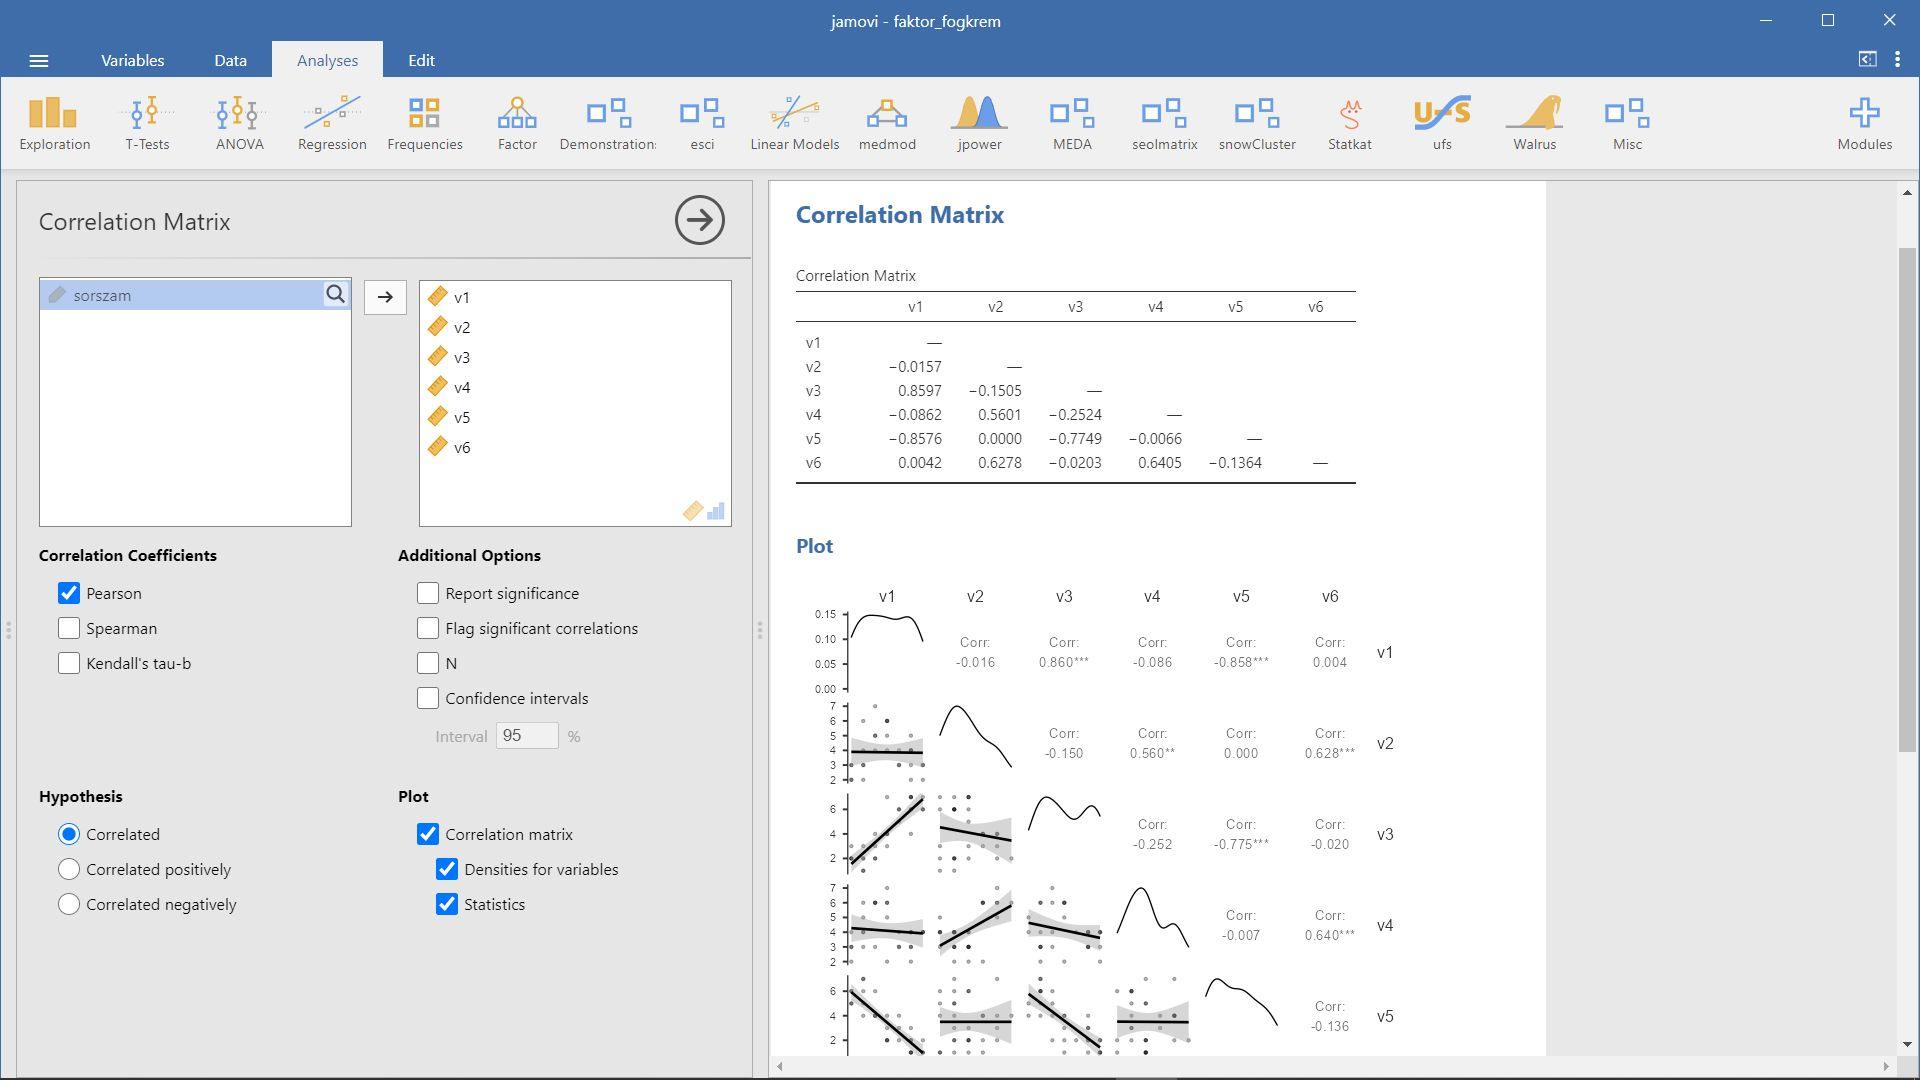
\includegraphics{./images/efa_fogkrem_01.jpg}

}

\caption{Korrelációs mátrix}

\end{figure}

A fogkrémvásárlás során keresett előnyök korrelációs mátrix
tanulmányozásával látható:

\begin{itemize}
\tightlist
\item
  viszonylag magas a korreláció a v1 (fogszuvasodás megelőzése), v3
  (erős fogíny) és v5 (a fog romlásának megelőzése) között. Arra
  számítunk, hogy ezek a változók ugyanazokkal a faktorokkal fognak
  korrelálni.
\item
  viszonylag magas a korreláció a v2 (fényes fogak), v4 (friss lehelet)
  és v6 (szép fogak) változók között, ezek is feltehetőleg ugyanazokkal
  a faktorokkal fognak korrelálni.
\end{itemize}

\textbf{3. Az alkalmazási feltételek ellenőrzése}

Ahhoz, hogy a faktorelemzés alkalmazható legyen, a változóknak
korrelálniuk kell egymással. Erről meggyőződhetünk kétféle objektív
módszerrel is:

\begin{itemize}
\tightlist
\item
  Bartlett-féle szferikus próba: nullhipotézise szerint a korrelációs
  mátrix egységmátrix (a változók korrelálatlanok), azaz az átlón kívül
  minden elem nulla. Amennyiben a nullhipotézis nem vethető el, a
  faktorelemzés alkalmazhatósága megkérdőjelezhető.
\item
  Kaiser-Meyer-Olkin-féle megfelelőségi mutató: a megfigyelt korrelációs
  együtthatók nagyságát viszonyítja a parciális korrelációs együtthatók
  nagyságához. Az alacsony KMO-mutató azt jelzi, hogy a változópárok
  közötti korreláció nem magyarázható más változókkal, így a
  faktorelemzés nem megfelelő módszer. Általában 0,5 fölött érték
  kívánatos.
\end{itemize}

Jamovi-ban a \texttt{Factor\ /\ Exploratory\ Factor\ Analysis}
menüpontban tudjuk a fenti vizsgálatokat elvégezni.

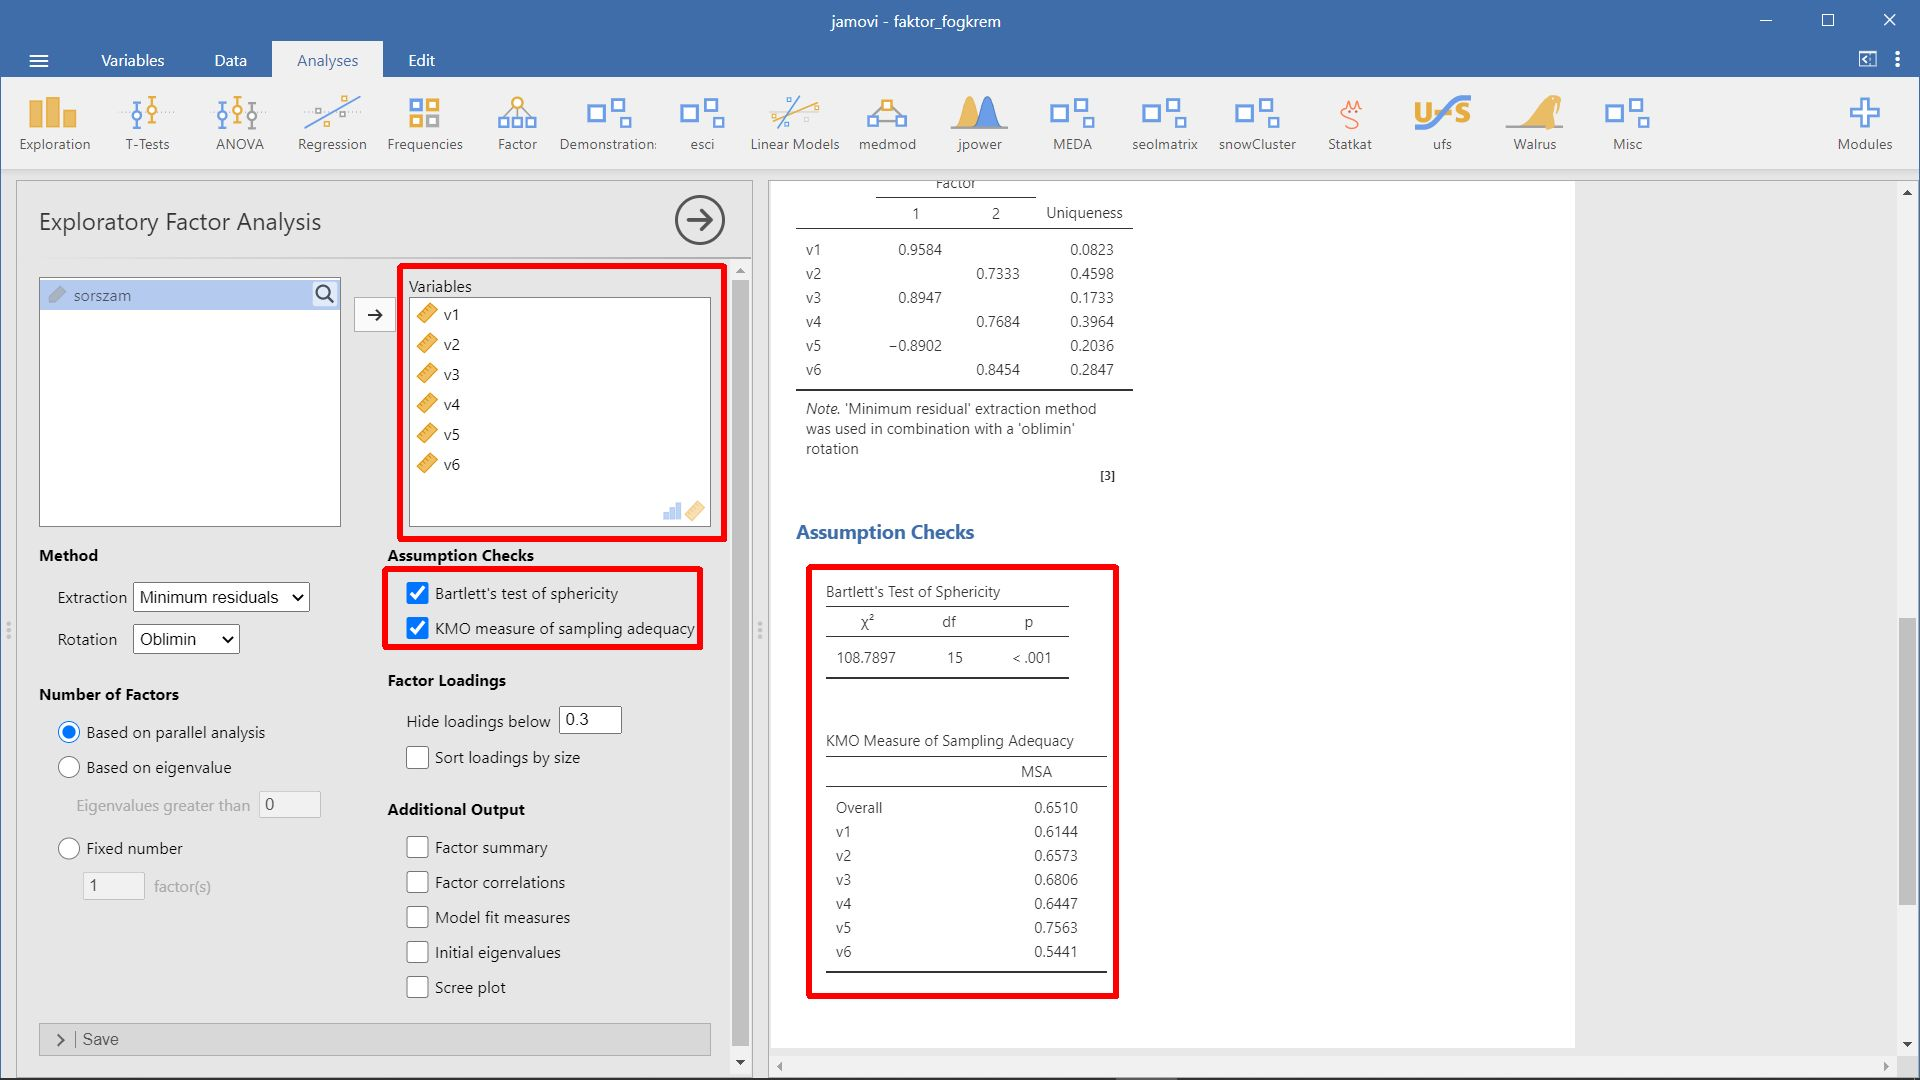
\includegraphics{./images/efa_fogkrem_02.jpg} A Bartlett-féle szferikus
próba szerint a pupulációban a korrelációs mátrix nem egységmátrix (ez
számunkra kedvező), valamint a KMO-érték 0,66, ameéy elég magas
(\textgreater0,5), így megállapíthatjuk, hogy a faktorelemzés alkalmas
módszer a korrelációs mátrix elemzésére.

\textbf{4. A faktorelemzés módszerének meghatározása}

A faktorelemzés egyes módszerei abban különböznek egymástól, hogy milyen
módon határozzák meg a súlyokat vagy faktorérték együtthatókat.

A jamovi 3 módszert ismer a közös faktorok becslésére:

\begin{itemize}
\tightlist
\item
  Principal axis -- főtengelyelemzés
\item
  Minimum residuals
\item
  Maximum likelihood
\end{itemize}

\textbf{5. A faktorok számának meghatározása}

A faktorelemzés akkor ér célt, ha a változók számánál kevesebb számú
közös faktort hozunk létre. De mi legyen ez a szám. Több eljárás
létezik. Ezeket részletesen a főkomponens elemzés során bemutattuk. Itt
csak felsoroljuk őket:

\begin{itemize}
\tightlist
\item
  Horn-féle párhuzamos analízis (jamovi-ban:
  \texttt{Based\ on\ parallel\ analysis})
\item
  A priori meghatározás (jamovi-ban: \texttt{Fixed\ number})
\item
  Sajátértéken alapuló megoldás (jamovi-ban:
  \texttt{Based\ on\ eigenvalue})
\item
  Sajátértékábrán (scree-plot, kőtörmelék ábra) alapuló meghatározás
  (jamovi-ban: \texttt{Scree\ plot})
\item
  Magyarázott varianciahányadon alapuló meghatározás (jamovi-ban:
  \texttt{Component\ summary})
\end{itemize}

\textbf{6. A faktorok forgatása}

A faktorelemzés fontos eredménye a faktormátrix (jamovi-ban:
\texttt{Factor\ Loadings}).

\begin{figure}

{\centering 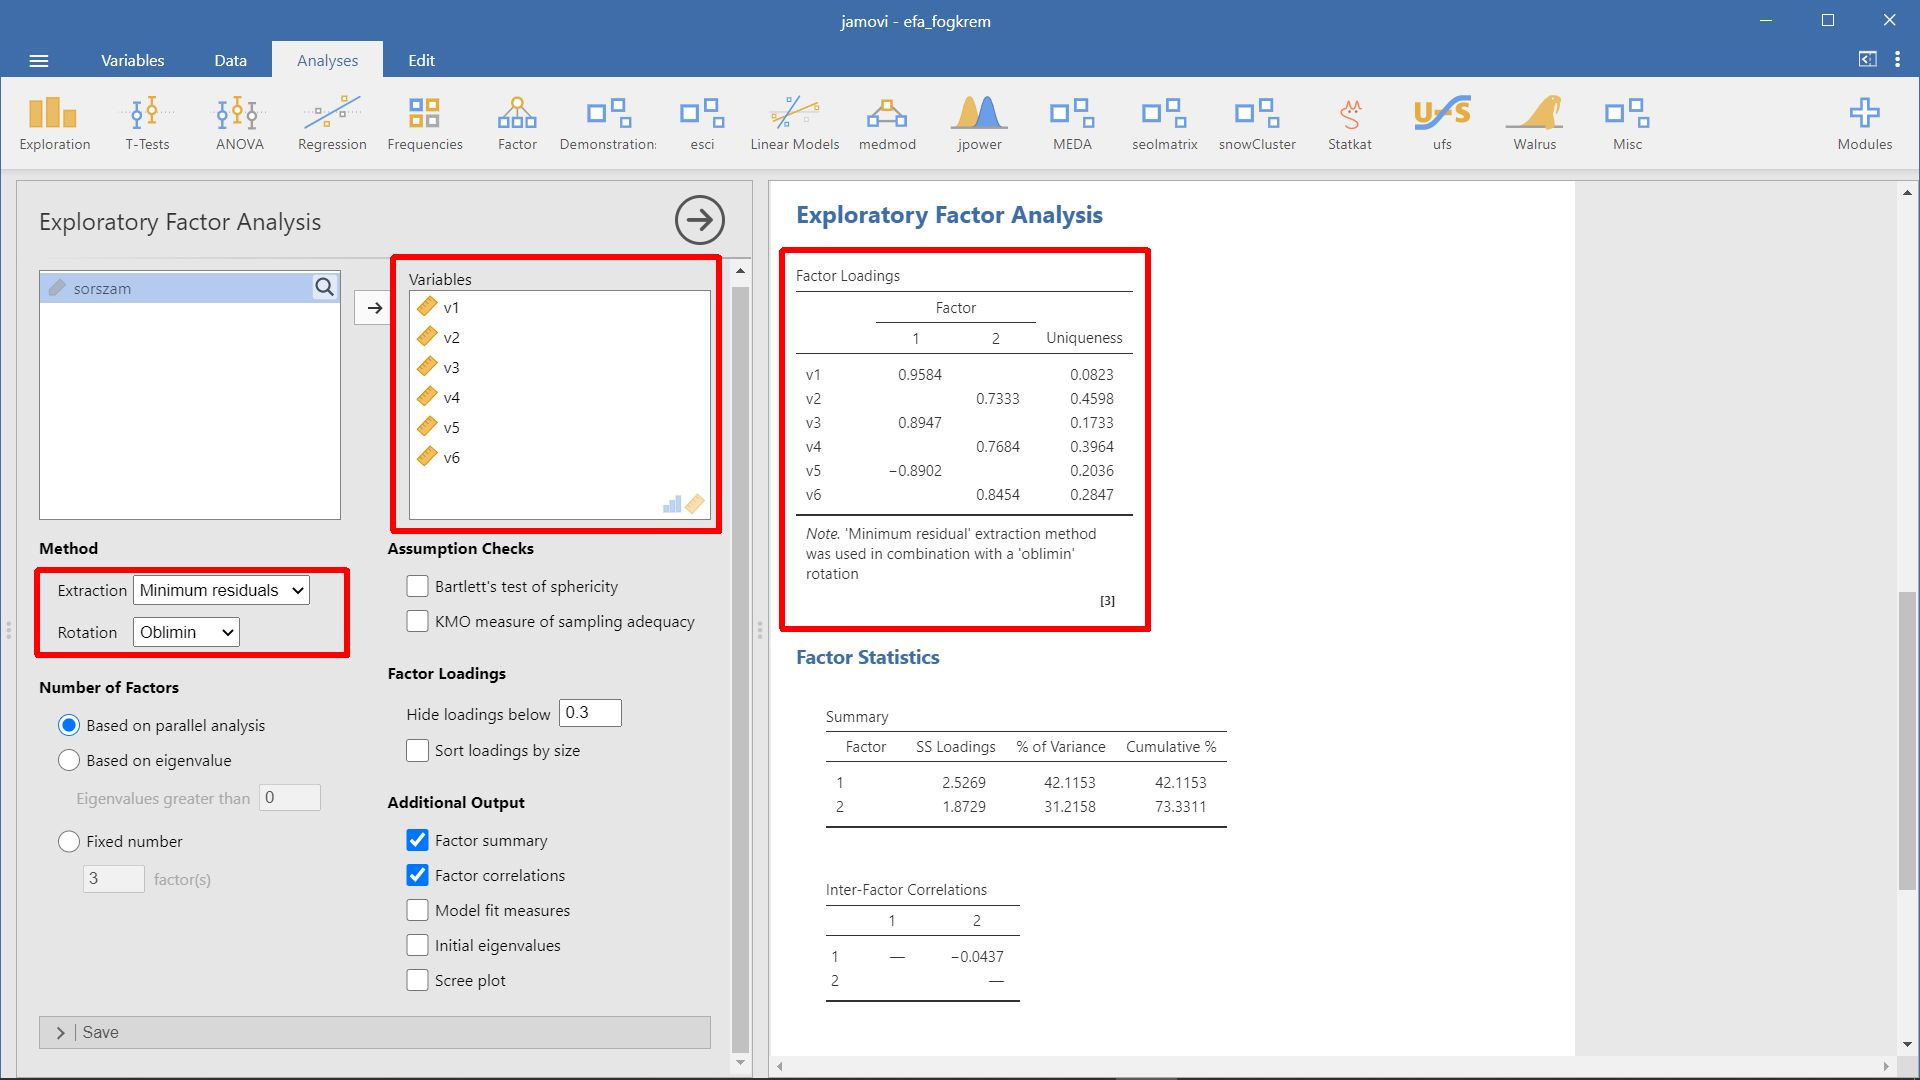
\includegraphics{./images/efa_fogkrem_03.jpg}

}

\caption{A faktormátrix}

\end{figure}

A faktormátrix tartalmazza azokat az együtthatókat, amelyekkel a
standardizált változókat ki lehet fejezni a faktorokkal. Ezeket az
együtthatókat faktorsúlyoknak nevezzük, a faktorok és a faktorsúlyok
közötti korrelációt mutatják. A magas abszolút értékű együttható azt
jelzi, hogy a faktor és a változó szorosan összefügg. A faktormátrix
együttható alapján lehet a faktorokat értelmezni.

A kiinduló vagy rotálatlan faktormátrix jelzi ugyan az egyes változók és
a faktorok kapcsolatát, de ritkán eredményez könnyen értelmezhető
faktorokat. Ennek főképp az az oka, hogy a faktorok túl sok változóval
korrelálnak. (A rotálatlan faktormátrix beállításához jamovi-ban a
\texttt{Rotation:\ None} beállítást használjuk.)

A faktorok forgatásával a faktormátrix egyszerűbbé, könnyebben
értelmezhetővé válik. A faktorok forgatásával szeretnénk elérni:

\begin{itemize}
\tightlist
\item
  minden faktor csak néhány vátozóra rendelkezzen szignifikánsan nem
  nulla súllyal
\item
  minden változónak lehetőleg egy faktorral legyen nem nulla, azaz
  szignifikáns faktorsúlya.
\end{itemize}

A forgatás nem érinti a kommunalitásokat és a magyarázott
varianciahányadot, azonban az egy faktor által magyarázott
varianciahányad változik (és természetesen a faktorsúlyok is).

A forgatási módszereket érdemes jól megválasztani, mert más-más faktorok
azonosításához vezetnek.

Az ortogonális (derékszögű) forgatási eljárások egymással nem korreláló
faktorokat eredményeznek.

\begin{itemize}
\item
  Ezek közül az egyik legnépszerűbb a Varimax eljárás, amely
  minimalizálja a nagy faktorsúllyal rendelkező változók számát, így
  segíti a faktorok értelmezését. A magyarázott variancia egyenletesen
  próbálja elosztani a faktorok között.
\item
  A Quartimax eljárás első faktorként egy általános faktort faktort hoz
  létre, amellyel szinte mindegyik változó magasan korrelál.
\end{itemize}

A ferdeszögű forgatási eljárások során a tengelyek hegyeszöget zárnak be
egymással, és a kapott faktorok korrelálni fognak egymással. Ferdeszögű
forgatást akkor kell használni, ha feltételezhető, hogy a sokaságban a
faktorok erősen összefüggenek.

\begin{itemize}
\item
  A Promax eljárás gyorsan lefuttatható, amely főképp nagy
  adatbázisoknál jelent előnyt.
\item
  A Simplimax a Promax egy módosított formája.
\item
  Az Oblimin eljárás a tengelyek egymással bezárt szögét fokozatosan
  változtatja, ami egyben a faktorok korreláltságát is meghatározza.
\end{itemize}

\textbf{7. A faktorok értelmezése}

Az értelmezést megkönnyíti, ha meghatározzuk azokat a változókat,
amelyeknek ugyanazon a faktorra nagy a súlyuk. A faktort a magas
faktorsúlyú változók alapján lehet értelmezni.

Az 1. faktornak magasabb az együtthatói a v1 (fugszuvasodás megelőzése),
v3 (erős fogíny) változókkal, negatív az együttható a v5 (a fog
romlásának megeleőzése nem fontos) változó esetében. Ezt a faktort az
``egészséggel kapcsolatos előnyöknek'' nevezhetjük. A 2. faktor a v2
(fényes fogak), a v4 (friss lehelet), v6 (szép fogak) változókkal függ
össze. Ezt a 2. faktort ``társadalmi előnyök''-nek nevezhetjük.

Összegezve, a fogyasztók feltehetőleg két fő előnyt keresnek a
fogkrémvásárlás során: egészséggel kapcsolatos és társadalmi előnyöket.

\textbf{8. A faktorértékek kiszámítása}

A faktorelemzésnek önmagában is van értelme, hiszen látens változók
azonosításához vezet, azonban hasznos lehet a későbbi elemzések számára
a faktorértékek kiszámítása minden egyes megkérdezettre. A faktor az
eredeti változók lineáris kombinációja. A standardizált változó
értékeinek és a megfelelő faktorérték-együtthatónak a szorzata adja a
faktorétéket, amely jelen példában minden válaszadóra két faktorértéket
jelent. A faktorérték csak főkomponens elemzés esetében lehet pontosan
kiszámítani, egyébként csak közelítő értékeket kapunk.

\begin{figure}

{\centering 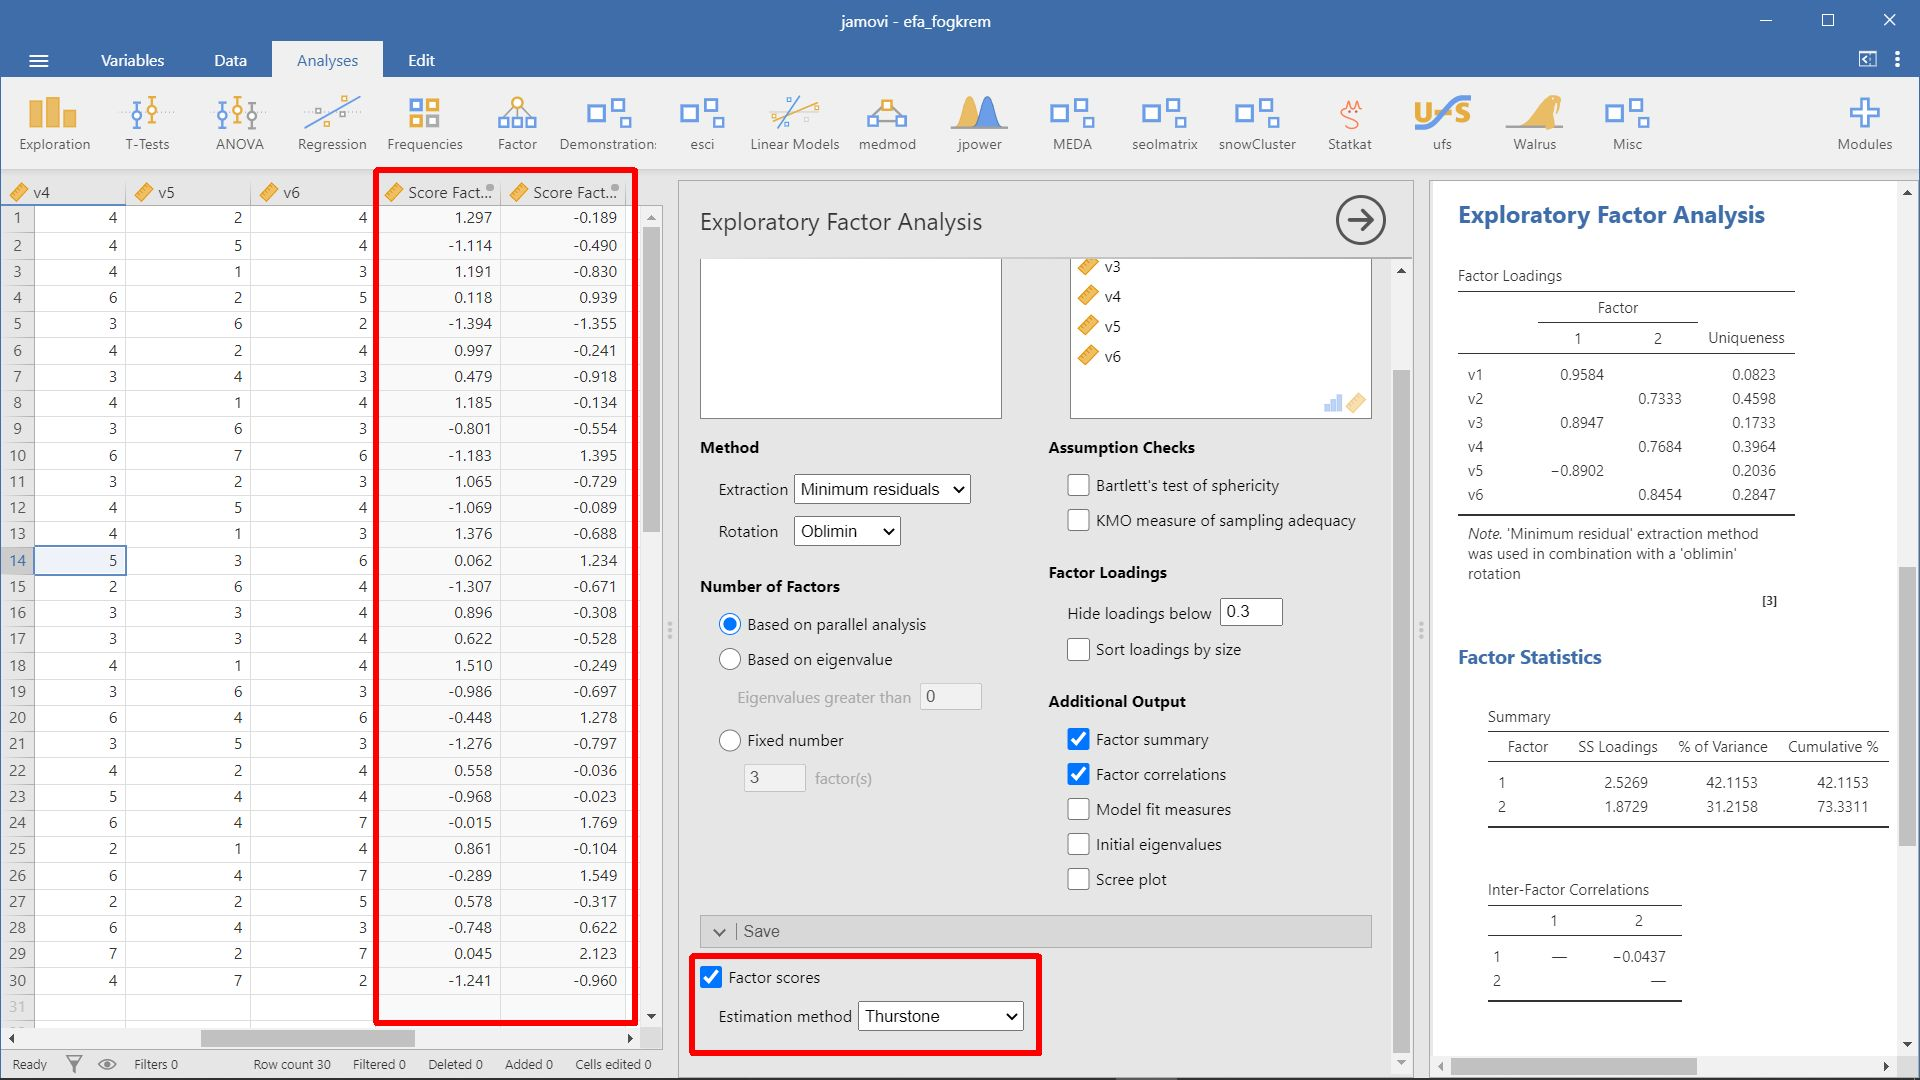
\includegraphics{./images/efa_fogkrem_04.jpg}

}

\caption{Faktorértékek kiszámítása}

\end{figure}

\hypertarget{illeszkeduxe9si-mutatuxf3k}{%
\section{Illeszkedési mutatók}\label{illeszkeduxe9si-mutatuxf3k}}

\begin{itemize}
\item
  \textbf{CFI} - összehasonlító illeszkedési mutató (Comparative Fit
  Index) - A CFI azt méri fel, hogy egy feltételezett hipotetikus modell
  milyen mértékben reprodukálja a valós adatokon nyugvó
  kovarianciamátrixot egy független modellhez képest.
\item
  \textbf{TLI} - Tucker--Lewis-féle Illeszkedési mutató - A TLI a
  CFI-hez hasonló módon méri az illeszkedést, annyi különbséggel, hogy
  ez a mutató a modellben használt szabadságfokot is figyelembe veszi,
  így kiküszöböli a vizsgálati minta méretének befolyásoló szerepét
\end{itemize}

A CFI és TLI mutatók értéke 0 és 1 közötti tartományba eshet, ahol az
1-hez közeli érték jelzi a szoros illeszkedést. Kezdetben a mutatók
elfogadhatósági kritériumának 0,90-et adtak meg, de az utóbbi időkben
inkább a 0,95-ot tekintik az elfogadhatóság alsó határának.

\begin{itemize}
\tightlist
\item
  \textbf{RMSEA} - a becslési hiba négyzetes átlagának gyöke
  (Root-Mean-Square Error of Approximation) - A Steiger-féle RMSEA
  mutatót a modell populációs kovariancia mátrixhoz viszonyított
  illeszkedésének becsléséhez használjuk. Az RMSEA az elemszámtól
  függetlenül hasonlítja össze, hogy a valós és az optimális
  paraméterekkel rendelkező hipotetikus modell kovarianciamátrixa milyen
  mértékben illeszkedik. Az RMSEA a modell takarékosságának megbízható
  jelzője, a komplex modellek hibás specifikálásának hatékony mutatója.
  Az RMSEA értéke is 0 és 1 közé eshet, itt azonban a kisebb, 0-hoz
  közel eső érték jelzi a jobb illeszkedést. Browne és Cudeck (1993)
  szerint az RMSEA értékei 0,05-ig szoros illeszkedést jeleznek; 0,08-os
  értékig pedig megfelelő illeszkedést, elfogadható populáción belüli
  becslési hibákkal.
\end{itemize}

\textbf{Model Test}

Az adatok és a teoretikus modell egybeesésének vizsgálata. Az egyik
leggyakrabban használt illeszkedési mutató a \(\chi^2\)-próba mértéke,
amelyet általában akkor tekinthetünk elfogadhatónak, ha a
szabadságfokhoz viszonyított értéke alacsony (pl. kisebb, mint a
szabadságfok kétszerese) és nem szignifikáns (p \textgreater{} 0,05).
Ennek a mutatónak azonban több korlátja létezik. A legjellemzőbbek a
többváltozós normalitás sérülésére és a mintanagyságra való érzékenység.
Számos empirikus eredmény és szimulációs vizsgálat támasztja alá, hogy a
normalitás sérülésekor vagy nagy elemszámú minta esetében a
\(\chi^2\)-próba kevésbé informatív, és a legtöbb esetben a modell
elvetését jelzi. A mintanagyságból fakadó korlátot gyakran a
\(\chi^2\)-próba szabadságfokhoz mért arányával próbálják kompenzálni
(\(\chi^2\)/szabadságfok), amelynek ugyan nincs pontos kritériuma, de az
ajánlások általában 2-től 5-ig terjednek, és a határérték alatti érték
jelez megfelelő illeszkedést.

\begin{figure}

{\centering 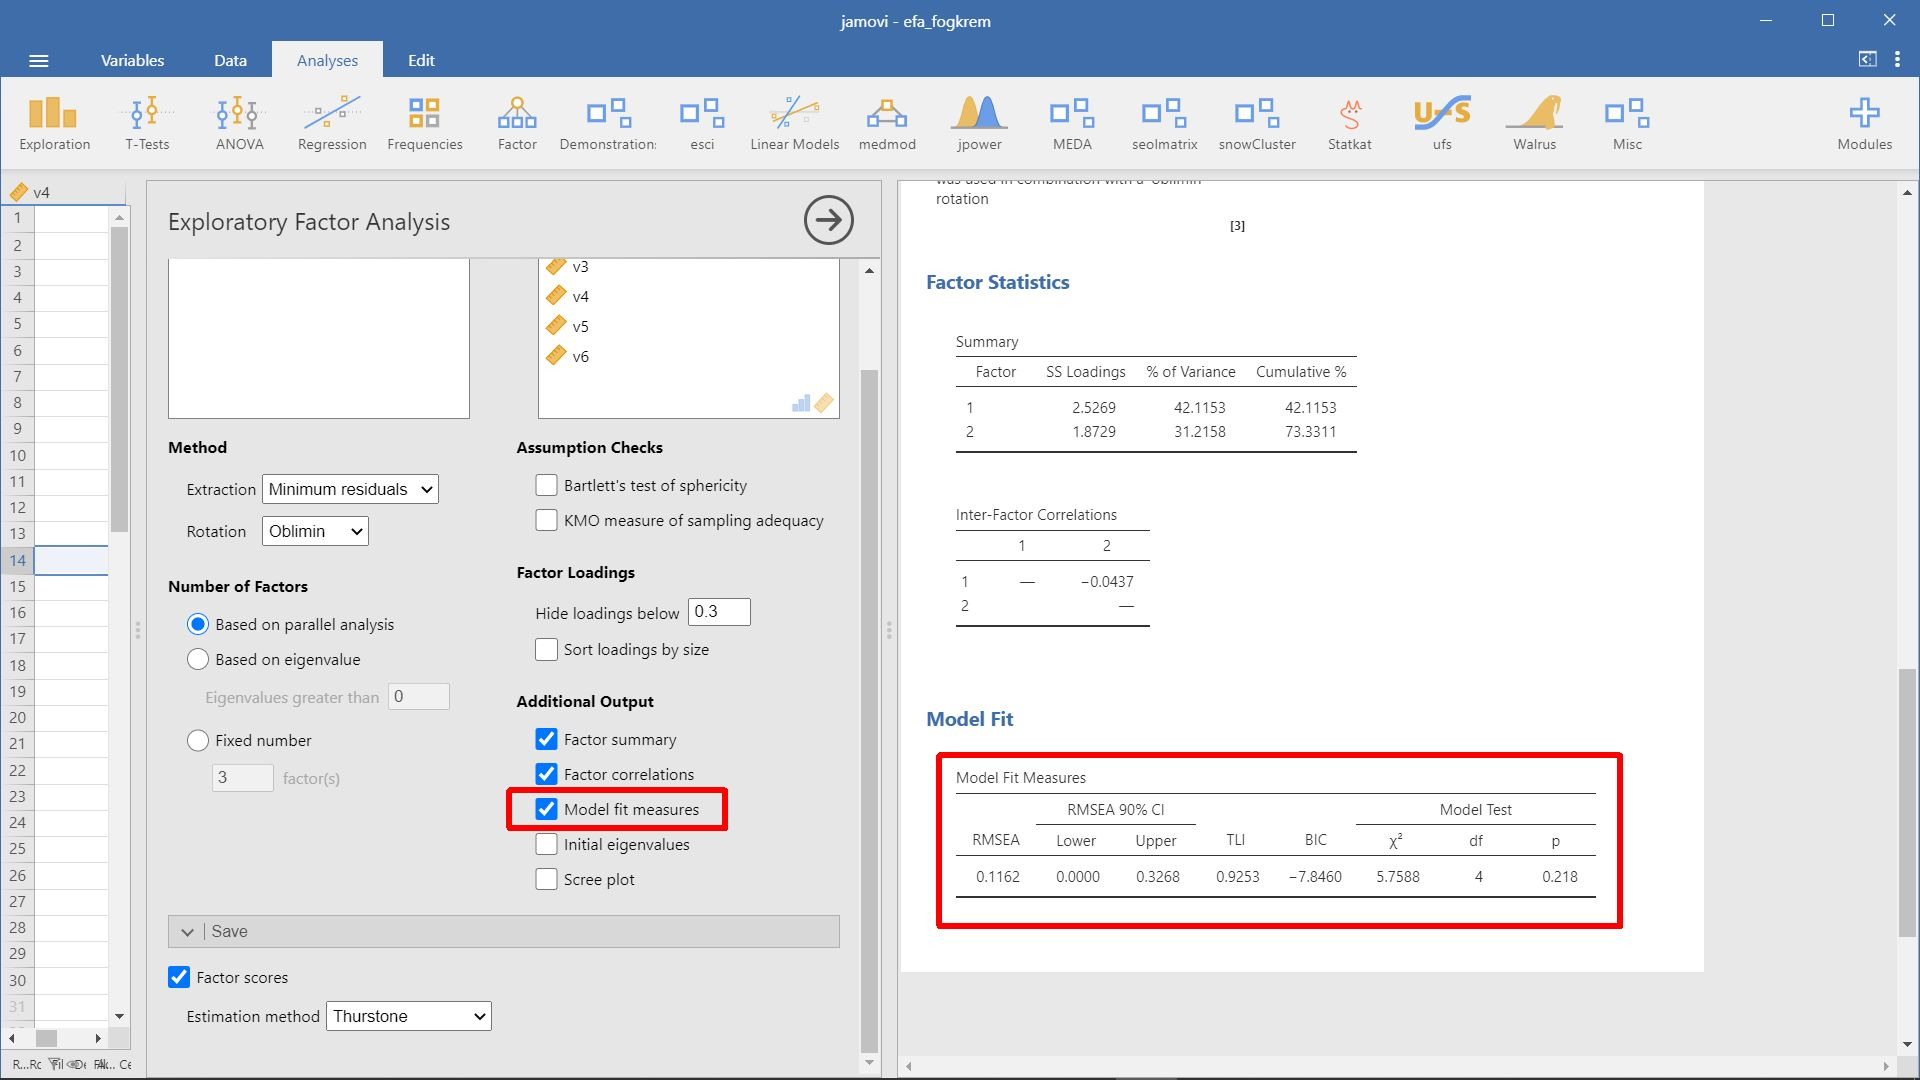
\includegraphics{./images/efa_fogkrem_05.jpg}

}

\caption{Illeszkedési mutatók}

\end{figure}

\hypertarget{puxe9lda-3}{%
\section{1. Példa}\label{puxe9lda-3}}

Valóban szétválasztható a reál és a humán tárgyakhoz szükséges tudás?

Összefoglalva, az adatokra jól illeszkedik a kétfaktoros modell, vagyis
azonosíthatjuk a humán és a reál tárgyakat az egyes tantárgyakból
nyújtott eredmények alapján. Az egyes tárgyak faktorba történő
besorolása összhangban van „hétköznapi'', előzetes tudásunkkal: a matek,
informatika és a kémia sorolható a reál, míg az irodalom, nyelvtan és
angol tárgyak a humán tárgyakhoz.

\hypertarget{puxe9lda-4}{%
\section{2. Példa}\label{puxe9lda-4}}

Milyen dimenziói vannak a kockázatvállalásnak és változik-e a korral a
kockázatvállalás?

A példák is mutatják, hogy a kockázatvállalásokat csoportosíthatjuk a
kockázatot jelentő tényezők alapján, ahol az egyik csoportban az emberek
saját testi épségüket teszik kockára (mint az autóversenyzés esetében),
de kockáztathatnak pénzt vagy valamilyen becsületbeli dolgot is (mint a
kártyázás és a blöffölés esetében). Példánkban megnézzük, hogy a
faktoranalízis alátámasztja-e feltevésünket, majd a faktoranalízis
eredményeit felhasználva megnézzük, hogy a kockázatvállaló viselkedésre
hatással van-e a kor.

Az adatbázisban szereplő adatokat úgy kaptuk, hogy a vizsgálati
személyeknek különböző foglalkozású, illetve különböző tevékenységet
végző embereket kellett megítélniük, hogy mennyire tartják őket
szimpatikusnak egy 1-7 skálán, ahol a 7 jelentette azt, hogy nagyon
szimpatikus. Ily módon megkaptuk a személyek kockázat iránti attitűdjét.
A változók között olyan személyek szerepelnek, mint kártyajátékosok,
autóversenyzők, üzletemberek (akik sok pénzt kockáztatnak), veszélyes
sportot űző emberek, nagy pénzekben fogadó emberek, blöffölők és
hivatásos katonák.

Ezen kívül két adat szerepel az adatbázisban: a nem és a kor.

Összefoglalva, sikerült a faktoranalízissel alátámasztanunk a
kockázatvállalás két faktorát. Azt is megállapítottuk, hogy mindkét
faktor függ a kortól: az anyagi/erkölcsi téren vállalt kockázat iránti
attitűd az évek múlásával egyre kedvezőbbé válik, míg a testi épség
terén vállalt kockázat iránti attitűd idővel egyre elutasítóbbá válik.

\hypertarget{puxe9lda-5}{%
\section{3. Példa}\label{puxe9lda-5}}

Egy kérdőív szerkesztésének problémái

Egy jó kérdőív kialakítása hosszas és nagyon alapos munkát igényel.
Egyik lépése, hogy megnézzük, az itemek valóban egy dimenzióra
illeszkednek-e. A nem odaillő itemeket pedig kivesszük a kérdőívből
(itemszelekció). Ennek módszerei lehetnek a korábban már tárgyalt
Cronbach-alfa, illetve ha főkomponens-analízist végzünk az itemekkel,
akkor a Theta is. A következőkben egy főkomponens-analízisen és
Cronbach-alfán alapuló itemszelekcióra nézünk példát.

\bookmarksetup{startatroot}

\hypertarget{sec-megerosito-faktorelemzes}{%
\chapter{Megerősítő faktorelemzés}\label{sec-megerosito-faktorelemzes}}

Tehát az a kísérletünk, hogy az EFA segítségével azonosítsuk a mögöttes
látens tényezőket a személyiségi elemkészletből gondosan kiválasztott
kérdésekkel, meglehetősen sikeresnek tűnt. A személyiség hasznos
mérőszámának kidolgozására irányuló törekvésünk következő lépése az
eredeti EFA-ban azonosított látens tényezők ellenőrzése egy másik
mintán. Azt akarjuk látni, hogy a tényezők helytállóak-e, meg tudjuk-e
igazolni létezésüket különböző adatokkal. Ez egy szigorúbb ellenőrzés,
mint látni fogjuk. És ezt Confirmatory Factor Analysisnek (CFA) hívják,
mivel nem meglepő módon egy előre meghatározott látens faktorstruktúra
megerősítésére törekszünk.

A CFA-ban ahelyett, hogy olyan elemzést végzünk, amelyben az adatok
feltáró értelemben vett együttállását látjuk, ehelyett struktúrát írunk
elő, mint a 15.13. ábrán, és megnézzük, hogy az adatok mennyire
illeszkednek az előre megadott struktúránkhoz. Ebben az értelemben egy
megerősítő elemzést végzünk, hogy megnézzük, mennyire erősítik meg a
megfigyelt adatok egy előre meghatározott modellt.

A személyiségelemek egyszerű megerősítő faktoranalízise (CFA) ezért öt
látens faktort határoz meg, amint azt a 15.13. ábra mutatja, mindegyiket
öt megfigyelt változóval mérve. Mindegyik változó egy mögöttes látens
tényező mértéke. Például az A1-et a mögöttes látens egyetértési tényező
előrejelzi. És mivel A1 nem tökéletes mértéke az elfogadhatósági
tényezőnek, van egy hibatag, , kapcsolódik hozzá. Más szavakkal, az A1
eltérését jelenti, amelyet az egyetértési tényező nem vesz figyelembe.
Ezt néha mérési hibának nevezik.

\bookmarksetup{startatroot}

\hypertarget{sec-tobbszempontos-varianciaelemzes}{%
\chapter{Többszempontos
varianciaelemzés}\label{sec-tobbszempontos-varianciaelemzes}}

JÖN.

\bookmarksetup{startatroot}

\hypertarget{sec-klaszterelemzes}{%
\chapter{Klaszterelemzés}\label{sec-klaszterelemzes}}

Az klaszterelemzés segítségével vizsgált probléma a következő: egy \(n\)
elemű adatbázisban minden egyes elemhez \(p\) darab változó értékei
kapcsolódnak; alakítsunk az elemekből csoportokat úgy, hogy a
``hasonlóak'' egy csoportba kerüljenek. Minden klaszter elemei
viszonylag hasonlóak legyenek egymáshoz, de különbözzenek más klaszterek
elemeitől.

Számos eljárás született a klaszteranalízis módszerén belül. Ebben a
könyvben két eljárással foglalkozunk részletesen:

\begin{itemize}
\tightlist
\item
  a hierarchikus eljárásokkal és a
\item
  K-középpontú klaszteranalízissel.
\end{itemize}

\hypertarget{hierarchikus-eljuxe1ruxe1sok}{%
\section{Hierarchikus eljárások}\label{hierarchikus-eljuxe1ruxe1sok}}

A hierarchikus eljárások az egyes személyek, objektumok, esetek közötti
távolság meghatározásával kezdődnek. A csoportok, klaszterek kialakítása
történhet összevonáson vagy felosztáson alapuló módszerekkel. Az
összevonó módszerek abból indulnak ki, hogy minden egyes elem egy önálló
csoportot alkot, majd fokozatosan vonják össze az egyelemes csoportokat
egyetlen nagy csoportba. Ezzel szemben a lebontó módszerben az összes
elem egyetlen csoportba tartozik, és ezt a csoportot osztjuk fel kettő,
majd egyre több csoportra addig, amíg minden elem egy önálló csoportot
nem alkot. Az összevonó módszernél kezdetben minden egyes elem külön
klasztert alkot. A klaszterek a megfigyelési egységek egyre nagyobb
klaszeterekbe csoportosításával alakulnak ki. A folyamat addig
folytatódik, amíg egyetlen klaszter lesz az egész. A következőkben a
legelterjedtebb klaszteralkotó módszereket soroljuk fel:

\begin{itemize}
\tightlist
\item
  Egyszerű lánc, avagy a legközelebbi szomszéd elve
\item
  Teljes lánc, avagy a legtávolabbi szomszéd elve
\item
  Átlagos távolság
\item
  Variancia-módszerek
\item
  Ward-féle eljárás
\item
  Centroidmódszerek
\item
  Szekvenciális küszöbérték módszer
\item
  Párhuzamos küszöbérték módszer
\item
  Optimális felosztás módszere
\end{itemize}

Jamovi-ban a \texttt{snowCluster} csomag segítségével végethetünk
klaszterelemzéseket. A csomag telepítése után a
\texttt{snowCluster\ /\ Hiearchical\ Clustering} vagy
\texttt{snowCluster\ /\ Clustering\ Dendogram} menüpontokat használjuk.

A jamovi a következő módszereket ismeri:

\begin{itemize}
\tightlist
\item
  ward.D
\item
  ward.D2
\item
  single
\item
  complete
\item
  average
\end{itemize}

\hypertarget{k-kuxf6zuxe9ppontuxfa-klaszterelemzuxe9s}{%
\section{K-középpontú
klaszterelemzés}\label{k-kuxf6zuxe9ppontuxfa-klaszterelemzuxe9s}}

JÖN.

\bookmarksetup{startatroot}

\hypertarget{sec-diszkriminancia-elemzes}{%
\chapter{Diszkriminancia elemzés}\label{sec-diszkriminancia-elemzes}}

A diszkriminancia analízisben azt a problémát járjuk körül, hogyan lehet
az emberek egyes csoportjait valamilyen vizsgált jellemzők alapján
szétválasztani, az egyes csoportokat azonosítani, valamint a
csoporttagságokat az előbb említett vizsgált jellemzők alapján
előrejelezni.

Képzeljünk el, hogy szalagmunkásokkal végeznek alkalmasság-vizsgálatot.
A szalagmunka általában sok figyelmet igényel, ugyanakkor meglehetősen
monoton munka, éppen ezért jó figyelmi képességek és monotónia tűrés
szükséges hozzá. A lenti \texttt{szalagmunka} adatmátrix 10 személy
adatát tartalmazza.

\begin{Shaded}
\begin{Highlighting}[]
\NormalTok{szalagmunka }\OtherTok{\textless{}{-}}\NormalTok{ rio}\SpecialCharTok{::}\FunctionTok{import}\NormalTok{(}\AttributeTok{file =} \StringTok{"adat/diszkriminancia\_alkalmassag.xlsx"}\NormalTok{)}
\NormalTok{szalagmunka}\SpecialCharTok{$}\NormalTok{bevalt }\OtherTok{\textless{}{-}} \FunctionTok{factor}\NormalTok{(szalagmunka}\SpecialCharTok{$}\NormalTok{bevalt, }\AttributeTok{labels =} \FunctionTok{c}\NormalTok{(}\StringTok{"nem"}\NormalTok{,}
    \StringTok{"igen"}\NormalTok{))}
\NormalTok{szalagmunka}
\CommentTok{\#\textgreater{}    bevalt figyelem monotonia\_tures}
\CommentTok{\#\textgreater{} 1    igen        1               2}
\CommentTok{\#\textgreater{} 2    igen        1               5}
\CommentTok{\#\textgreater{} 3     nem        2               1}
\CommentTok{\#\textgreater{} 4    igen        2               3}
\CommentTok{\#\textgreater{} 5     nem        3               2}
\CommentTok{\#\textgreater{} 6    igen        3               4}
\CommentTok{\#\textgreater{} 7     nem        4               3}
\CommentTok{\#\textgreater{} 8     nem        4               1}
\CommentTok{\#\textgreater{} 9    igen        4               6}
\CommentTok{\#\textgreater{} 10    nem        6               5}
\end{Highlighting}
\end{Shaded}

A fenti adatok egy részét a szalagmunkára való jelentkezéskor
gyűjtötték:

\begin{itemize}
\tightlist
\item
  \texttt{figyelem}: figyelmi képességükre és
\item
  \texttt{monotonia\_tures}: monotónia-tűrésükre vonatkozó információk.
\end{itemize}

Mindkét változót 7 fokú skálán értékeltek (ahol a magasabb érték jobb
képességeket jelent), valamint azt az információt is láthatjuk, hogy
később beváltak-e vagy sem (\texttt{bevalt}).

Azt kellene megmutatnunk, hogy a figyelem és a monotónia-tűrés
pontszámai alapján valóban lehet következtetést levonni a személy
beválását illetően. Ha ezt sikerül egy objektív statisztikai módszerrel
is igazolnunk, akkor az ezt követően szalagmunkára jelentkezőket
figyelem és monotónia tűréssel vizsgálva tesztelhetjük, és egész jól ki
lehet válogatni az alkalmasabb jelölteket.

Ha pontdiagramon ábrázoljuk az adatokat, és színezéssel jelöljük a
beválást, akkor a két csoport szemmel láthatóan szétválik egymástól, ám
sem a függőleges, sem a vízszintes tengely mentén nem lehet elkülöníteni
a csoportokat.

\begin{Shaded}
\begin{Highlighting}[]
\FunctionTok{library}\NormalTok{(ggplot2)}
\FunctionTok{ggplot}\NormalTok{(szalagmunka, }\FunctionTok{aes}\NormalTok{(}\AttributeTok{x =}\NormalTok{ figyelem, }\AttributeTok{y =}\NormalTok{ monotonia\_tures, }\AttributeTok{colour =}\NormalTok{ bevalt)) }\SpecialCharTok{+}
    \FunctionTok{geom\_point}\NormalTok{(}\AttributeTok{size =} \DecValTok{4}\NormalTok{)}
\end{Highlighting}
\end{Shaded}

\begin{figure}[H]

{\centering 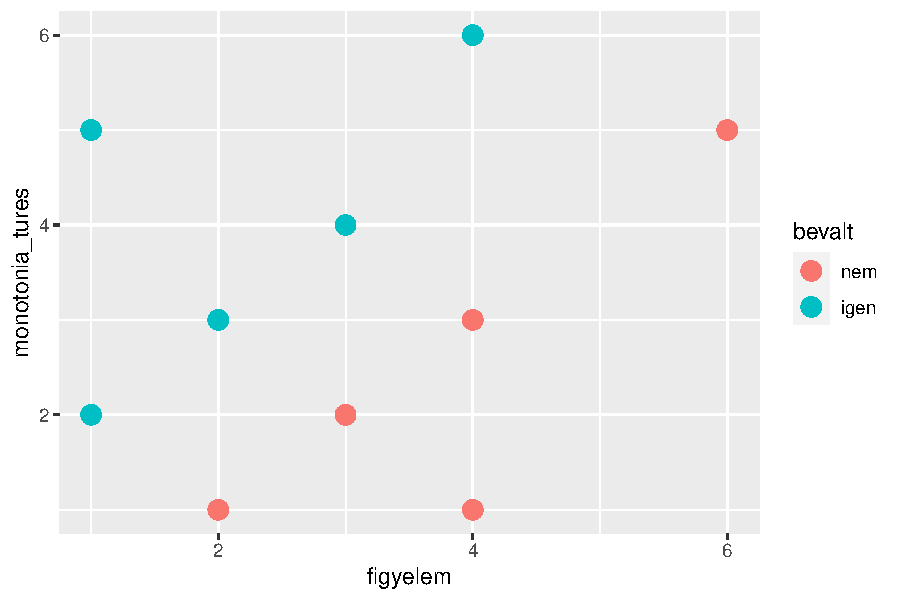
\includegraphics{./sec_diszkrimninancia_files/figure-pdf/unnamed-chunk-3-1.pdf}

}

\end{figure}

\textbf{A diszkriminancia elemzés sajátossága, hogy a csoportokat a
magyarázó változók együttes figyelembevételével tudja szétválasztani.}
Ennek megfelelően ha önmagában tekintjük az egyik (például
\texttt{figyelem}) vagy másik (\texttt{monotonia\_tures}) magyarázó
változókat, akkor nem tudunk szignifikáns különbséget kimutatni a
\texttt{bevalt} változó két csoportjában \((p = 0,108; p=0,159)\).

\begin{Shaded}
\begin{Highlighting}[]
\FunctionTok{t.test}\NormalTok{(figyelem }\SpecialCharTok{\textasciitilde{}}\NormalTok{ bevalt, }\AttributeTok{data =}\NormalTok{ szalagmunka)}\SpecialCharTok{$}\NormalTok{p.value}
\CommentTok{\#\textgreater{} [1] 0.1082333}
\FunctionTok{t.test}\NormalTok{(monotonia\_tures }\SpecialCharTok{\textasciitilde{}}\NormalTok{ bevalt, }\AttributeTok{data =}\NormalTok{ szalagmunka)}\SpecialCharTok{$}\NormalTok{p.value}
\CommentTok{\#\textgreater{} [1] 0.1588974}
\end{Highlighting}
\end{Shaded}

Nézzük meg, hogy többváltozós variancia-analízissel (MANOVA) szét
tudjuk-e választani a csoportokat, amikor a két magyarázó változót
egyszerre vesszük figyelembe. Továbbra is arra keressük a választ, hogy
beválás tekintetében valóban létezik-e a munkások két csoportja.

\begin{Shaded}
\begin{Highlighting}[]
\NormalTok{man\_1 }\OtherTok{\textless{}{-}} \FunctionTok{manova}\NormalTok{(}\FunctionTok{cbind}\NormalTok{(figyelem, monotonia\_tures) }\SpecialCharTok{\textasciitilde{}}\NormalTok{ bevalt, }\AttributeTok{data =}\NormalTok{ szalagmunka)}
\FunctionTok{summary}\NormalTok{(man\_1, }\AttributeTok{test =} \StringTok{"Wilks"}\NormalTok{)}
\CommentTok{\#\textgreater{}           Df  Wilks approx F num Df den Df  Pr(\textgreater{}F)  }
\CommentTok{\#\textgreater{} bevalt     1 0.2708   9.4247      2      7 0.01033 *}
\CommentTok{\#\textgreater{} Residuals  8                                        }
\CommentTok{\#\textgreater{} {-}{-}{-}}
\CommentTok{\#\textgreater{} Signif. codes:  }
\CommentTok{\#\textgreater{} 0 \textquotesingle{}***\textquotesingle{} 0.001 \textquotesingle{}**\textquotesingle{} 0.01 \textquotesingle{}*\textquotesingle{} 0.05 \textquotesingle{}.\textquotesingle{} 0.1 \textquotesingle{} \textquotesingle{} 1}
\end{Highlighting}
\end{Shaded}

A fenti output alapján megnyugodhatunk, a bevált és a nem bevált
munkások csoportja valóban különbözik egymástól \((p=0,010)\).

A diszkriminancia elemzéstől azonban ettől többet fogunk várni, például
predikciót is végezhetünk a kapott modellben.

Ha diszkriminancia elemzést szeretnénk végrehajtani, akkor a
\texttt{\{MASS\}} csomag \texttt{lda()} függvényét használhatjuk.

\begin{Shaded}
\begin{Highlighting}[]
\NormalTok{lda\_1 }\OtherTok{\textless{}{-}}\NormalTok{ MASS}\SpecialCharTok{::}\FunctionTok{lda}\NormalTok{(bevalt }\SpecialCharTok{\textasciitilde{}}\NormalTok{ figyelem }\SpecialCharTok{+}\NormalTok{ monotonia\_tures, }\AttributeTok{data =}\NormalTok{ szalagmunka)}
\NormalTok{lda\_1}
\CommentTok{\#\textgreater{} Call:}
\CommentTok{\#\textgreater{} lda(bevalt \textasciitilde{} figyelem + monotonia\_tures, data = sza...}
\CommentTok{\#\textgreater{} }
\CommentTok{\#\textgreater{} Prior probabilities of groups:}
\CommentTok{\#\textgreater{}  nem igen }
\CommentTok{\#\textgreater{}  0.5  0.5 }
\CommentTok{\#\textgreater{} }
\CommentTok{\#\textgreater{} Group means:}
\CommentTok{\#\textgreater{}      figyelem monotonia\_tures}
\CommentTok{\#\textgreater{} nem       3.8             2.4}
\CommentTok{\#\textgreater{} igen      2.2             4.0}
\CommentTok{\#\textgreater{} }
\CommentTok{\#\textgreater{} Coefficients of linear discriminants:}
\CommentTok{\#\textgreater{}                        LD1}
\CommentTok{\#\textgreater{} figyelem        {-}0.9981001}
\CommentTok{\#\textgreater{} monotonia\_tures  0.8365579}
\end{Highlighting}
\end{Shaded}

A fenti outputban látható, hogy akik nem váltak be, a monotónia-tűrés
tesztben gyengébb teljesítményt nyújtottak, a figyelem tesztben pedig
egy jobbat, míg akik beváltak, a monotónia-tűrés tesztben igen jó
teljesítményt értek el, a figyelem tesztben pedig valamivel gyengébbet.
A kanonikus diszkriminancia együtthatókat is láthatjuk, melyek alapján
felírhatjuk a kanonikus diszkriminancia-függvényt a következő módon:

\begin{Shaded}
\begin{Highlighting}[]
\NormalTok{Z = {-}0,998 * figyelem + 0,837 * monotonia\_tures}
\end{Highlighting}
\end{Shaded}

Az eddig vizsgált 10 személyről tudjuk, hogy bevált-e vagy sem, vagyis
ismertük a tényleges csoporttagságát. Ám a diszkriminancia elemzés
fontos célja, hogy előre jelezzük a csoporttagságokat, vagyis a figyelem
és monotónia-tűrés ismeretében megmondjuk egy személyről, hogy nagy
valószínűséggel beválik-e vagy sem.

Tegyük fel, hogy az első személy a figyelem teszten 2, míg a
monotónia-tűrés teszten 4 pontot kapott, míg a második személy
pontszámai ebben a sorrendben 6 és 1.

\begin{Shaded}
\begin{Highlighting}[]
\NormalTok{newdata }\OtherTok{\textless{}{-}} \FunctionTok{data.frame}\NormalTok{(}\AttributeTok{figyelem =} \FunctionTok{c}\NormalTok{(}\DecValTok{2}\NormalTok{, }\DecValTok{6}\NormalTok{), }\AttributeTok{monotonia\_tures =} \FunctionTok{c}\NormalTok{(}\DecValTok{4}\NormalTok{,}
    \DecValTok{1}\NormalTok{))}
\NormalTok{newdata}
\CommentTok{\#\textgreater{}   figyelem monotonia\_tures}
\CommentTok{\#\textgreater{} 1        2               4}
\CommentTok{\#\textgreater{} 2        6               1}
\NormalTok{lda\_1\_pred }\OtherTok{\textless{}{-}} \FunctionTok{predict}\NormalTok{(lda\_1, }\AttributeTok{newdata =}\NormalTok{ newdata)}
\NormalTok{lda\_1\_pred}
\CommentTok{\#\textgreater{} $class}
\CommentTok{\#\textgreater{} [1] igen nem }
\CommentTok{\#\textgreater{} Levels: nem igen}
\CommentTok{\#\textgreater{} }
\CommentTok{\#\textgreater{} $posterior}
\CommentTok{\#\textgreater{}          nem         igen}
\CommentTok{\#\textgreater{} 1 0.00743262 9.925674e{-}01}
\CommentTok{\#\textgreater{} 2 0.99999931 6.861874e{-}07}
\CommentTok{\#\textgreater{} }
\CommentTok{\#\textgreater{} $x}
\CommentTok{\#\textgreater{}         LD1}
\CommentTok{\#\textgreater{} 1  1.667346}
\CommentTok{\#\textgreater{} 2 {-}4.834728}
\end{Highlighting}
\end{Shaded}

A fenti output \texttt{class} és \texttt{posterior} része alapján
láthatjuk, hogy az első személyt nagy valószínűséggel alkalmasnak, míg a
másodikat alkalmatlannak ítélhetjük a szalagmunkára.

Utolsó lépésként összevetjük a tényleges és a becsült csoporttagságot,
és megállapítjuk, az adatok mekkora részét tudjuk helyesen besorolni az
alkotott modell alapján. Ezzel magát a modellt értékeljük.

\begin{Shaded}
\begin{Highlighting}[]
\NormalTok{lda\_2\_pred }\OtherTok{\textless{}{-}} \FunctionTok{predict}\NormalTok{(lda\_1, }\AttributeTok{method =} \StringTok{"plug{-}in"}\NormalTok{)}
\NormalTok{tab\_1 }\OtherTok{\textless{}{-}} \FunctionTok{table}\NormalTok{(lda\_2\_pred}\SpecialCharTok{$}\NormalTok{class, szalagmunka}\SpecialCharTok{$}\NormalTok{bevalt)}
\NormalTok{tab\_1}
\CommentTok{\#\textgreater{}       }
\CommentTok{\#\textgreater{}        nem igen}
\CommentTok{\#\textgreater{}   nem    5    0}
\CommentTok{\#\textgreater{}   igen   0    5}
\end{Highlighting}
\end{Shaded}

Mivel az összes adat a főátlóban van, így megállapíthatjuk, hogy a
modell alapján az összes adatot helyesen kategorizáltuk. A helyes
besorolás arányát százalékosan is kiszámíthatjuk, ez az arány 100\%.

\begin{Shaded}
\begin{Highlighting}[]
\DecValTok{100} \SpecialCharTok{*} \FunctionTok{sum}\NormalTok{(}\FunctionTok{diag}\NormalTok{(tab\_1))}\SpecialCharTok{/}\FunctionTok{sum}\NormalTok{(tab\_1)}
\CommentTok{\#\textgreater{} [1] 100}
\end{Highlighting}
\end{Shaded}

\hypertarget{puxe9lda-kikbux151l-lesznek-a-balesetezux151k}{%
\section{Példa: Kikből lesznek a
balesetezők?}\label{puxe9lda-kikbux151l-lesznek-a-balesetezux151k}}

Ebben a példában azt vizsgáljuk, mely tényezők járulnak hozzá a
balesetekhez.

\begin{Shaded}
\begin{Highlighting}[]
\NormalTok{baleset }\OtherTok{\textless{}{-}}\NormalTok{ rio}\SpecialCharTok{::}\FunctionTok{import}\NormalTok{(}\AttributeTok{file =} \StringTok{"adat/diszkriminancia\_baleset.xlsx"}\NormalTok{)}
\NormalTok{baleset}\SpecialCharTok{$}\NormalTok{baleset }\OtherTok{\textless{}{-}} \FunctionTok{factor}\NormalTok{(baleset}\SpecialCharTok{$}\NormalTok{baleset, }\AttributeTok{labels =} \FunctionTok{c}\NormalTok{(}\StringTok{"nem volt baleste"}\NormalTok{,}
    \StringTok{"volt baleste"}\NormalTok{))}
\FunctionTok{str}\NormalTok{(baleset)}
\CommentTok{\#\textgreater{} \textquotesingle{}data.frame\textquotesingle{}:    36 obs. of  5 variables:}
\CommentTok{\#\textgreater{}  $ baleset   : Factor w/ 2 levels "nem volt baleste...}
\CommentTok{\#\textgreater{}  $ megosztott: num  7 6 5 6 7 3 6 7 5 6 ...}
\CommentTok{\#\textgreater{}  $ pontossag : num  6 6 5 6 7 3 5 7 5 6 ...}
\CommentTok{\#\textgreater{}  $ kockazat  : num  2 3 1 2 4 7 2 1 3 2 ...}
\CommentTok{\#\textgreater{}  $ eszleles  : num  7 6 5 6 7 7 7 6 3 7 ...}
\NormalTok{psych}\SpecialCharTok{::}\FunctionTok{headTail}\NormalTok{(baleset)}
\CommentTok{\#\textgreater{}              baleset megosztott pontossag kockazat}
\CommentTok{\#\textgreater{} 1   nem volt baleste          7         6        2}
\CommentTok{\#\textgreater{} 2   nem volt baleste          6         6        3}
\CommentTok{\#\textgreater{} 3   nem volt baleste          5         5        1}
\CommentTok{\#\textgreater{} 4   nem volt baleste          6         6        2}
\CommentTok{\#\textgreater{} ...             \textless{}NA\textgreater{}        ...       ...      ...}
\CommentTok{\#\textgreater{} 33      volt baleste          3         3        5}
\CommentTok{\#\textgreater{} 34      volt baleste          2         2        7}
\CommentTok{\#\textgreater{} 35      volt baleste          3         3        4}
\CommentTok{\#\textgreater{} 36      volt baleste          4         4        6}
\CommentTok{\#\textgreater{}     eszleles}
\CommentTok{\#\textgreater{} 1          7}
\CommentTok{\#\textgreater{} 2          6}
\CommentTok{\#\textgreater{} 3          5}
\CommentTok{\#\textgreater{} 4          6}
\CommentTok{\#\textgreater{} ...      ...}
\CommentTok{\#\textgreater{} 33         4}
\CommentTok{\#\textgreater{} 34         1}
\CommentTok{\#\textgreater{} 35         4}
\CommentTok{\#\textgreater{} 36         4}
\end{Highlighting}
\end{Shaded}

Az adatbázisban a \texttt{baleset} változó azt rögzíti, hogy volt-e már
balesete a személynek vagy sem. Ez lesz tehát a csoportosító változó. A
többi változó, melyek segítségével próbáljuk a csoportok közötti
különbséget jellemezni, olyan dolgot mérnek, mint a megosztott figyelem
(\texttt{megosztott} változó), a figyelem pontossága
(\texttt{pontossag}), kockázatvállalási hajlandóság (\texttt{kockazat})
és az észlelés gyorsasága (\texttt{eszleles}).

A diszkriminancia-analízisben az első lépés annak megállapítása, vajon
valóban szét lehet-e választani a balesetezők és a nem balesetezők
csoportját az adott változók alapján. Ehhez a Wilks-lambda tesztet
használjuk a többváltozós variancia-analízis keretein belül.

\begin{Shaded}
\begin{Highlighting}[]
\NormalTok{man\_1 }\OtherTok{\textless{}{-}} \FunctionTok{manova}\NormalTok{(}\FunctionTok{cbind}\NormalTok{(megosztott, pontossag, kockazat, eszleles) }\SpecialCharTok{\textasciitilde{}}
\NormalTok{    baleset, }\AttributeTok{data =}\NormalTok{ baleset)}
\FunctionTok{summary}\NormalTok{(man\_1, }\AttributeTok{test =} \StringTok{"Wilks"}\NormalTok{)}
\CommentTok{\#\textgreater{}           Df   Wilks approx F num Df den Df    Pr(\textgreater{}F)}
\CommentTok{\#\textgreater{} baleset    1 0.27605   20.324      4     31 2.645e{-}08}
\CommentTok{\#\textgreater{} Residuals 34                                         }
\CommentTok{\#\textgreater{}              }
\CommentTok{\#\textgreater{} baleset   ***}
\CommentTok{\#\textgreater{} Residuals    }
\CommentTok{\#\textgreater{} {-}{-}{-}}
\CommentTok{\#\textgreater{} Signif. codes:  }
\CommentTok{\#\textgreater{} 0 \textquotesingle{}***\textquotesingle{} 0.001 \textquotesingle{}**\textquotesingle{} 0.01 \textquotesingle{}*\textquotesingle{} 0.05 \textquotesingle{}.\textquotesingle{} 0.1 \textquotesingle{} \textquotesingle{} 1}
\end{Highlighting}
\end{Shaded}

A fenti output tesztstatisztikájának szignifikanciaszintje azt mutatja,
hogy a csoportok közötti különbségek szignifikánsak, vagyis valóban van
különbség a balesetet szenvedett és a balesetmentes autóvezetők között.

Futtassuk le a diszkriminancia-analízis.

\begin{Shaded}
\begin{Highlighting}[]
\NormalTok{lda\_1 }\OtherTok{\textless{}{-}}\NormalTok{ MASS}\SpecialCharTok{::}\FunctionTok{lda}\NormalTok{(baleset }\SpecialCharTok{\textasciitilde{}}\NormalTok{ megosztott }\SpecialCharTok{+}\NormalTok{ pontossag }\SpecialCharTok{+}\NormalTok{ kockazat }\SpecialCharTok{+}
\NormalTok{    eszleles, }\AttributeTok{data =}\NormalTok{ baleset)}
\NormalTok{lda\_1}
\CommentTok{\#\textgreater{} Call:}
\CommentTok{\#\textgreater{} lda(baleset \textasciitilde{} megosztott + pontossag + kockazat + e...}
\CommentTok{\#\textgreater{} }
\CommentTok{\#\textgreater{} Prior probabilities of groups:}
\CommentTok{\#\textgreater{} nem volt baleste     volt baleste }
\CommentTok{\#\textgreater{}        0.4722222        0.5277778 }
\CommentTok{\#\textgreater{} }
\CommentTok{\#\textgreater{} Group means:}
\CommentTok{\#\textgreater{}                  megosztott pontossag kockazat eszl...}
\CommentTok{\#\textgreater{} nem volt baleste   5.941176  5.647059 2.588235 5.94...}
\CommentTok{\#\textgreater{} volt baleste       2.842105  2.684211 5.578947 3.10...}
\CommentTok{\#\textgreater{} }
\CommentTok{\#\textgreater{} Coefficients of linear discriminants:}
\CommentTok{\#\textgreater{}                    LD1}
\CommentTok{\#\textgreater{} megosztott {-}0.25764616}
\CommentTok{\#\textgreater{} pontossag  {-}0.07708289}
\CommentTok{\#\textgreater{} kockazat    0.36270659}
\CommentTok{\#\textgreater{} eszleles   {-}0.36702363}
\end{Highlighting}
\end{Shaded}

A fenti output alapján az előzetes valószínűsége annak, hogy valakinek
még nem volt balesete 0,472, míg annak a valószínűsége, hogy már volt
balesete a személynek 0,528. Ezután vizsgálhatjuk a csoportátlagokat. A
balesetmentes vezetők esetében magasabb a megosztott figyelem, a
figyelem pontosságának és az észlelés változójának az átlaga, míg a
kockázatvállalásé alacsonyabb. Ugyanakkor a másik csoport esetében a
kockázatvállalás változójának az átlaga magasabb, míg a másik három
képesség változójának átlaga alacsonyabb. Vagyis a balesetmentes vezetők
gyorsabban képesek észlelni és jobban meg tudják osztani a figyelmüket,
figyelmük pontosabb. A balesetet szenvedett vezetők esetében ezek a
képességek gyengébbek, míg jobban szeretnek kockázatot vállalni.

Végül a kanonikus diszkriminancia együtthatók segítségével felírhatjuk a
kanonikus diszkriminancia-függvényt a következő módon:

\begin{Shaded}
\begin{Highlighting}[]
\NormalTok{Z = 0,3627 * kockázat {-} 0,367 * észlelés {-} 0,2567 * megosztott{-}0,0771 * pontosság}
\end{Highlighting}
\end{Shaded}

Utolsó lépésként pedig megnézhetjük, mennyire hatékony a
diszkriminancia-analízis vagyis összevethetjük az eredeti
csoporttagságokat a modell alapján alkotott besorolásokkal.

\begin{Shaded}
\begin{Highlighting}[]
\NormalTok{lda\_1\_pred }\OtherTok{\textless{}{-}} \FunctionTok{predict}\NormalTok{(lda\_1, }\AttributeTok{method =} \StringTok{"plug{-}in"}\NormalTok{)}
\NormalTok{tab\_1 }\OtherTok{\textless{}{-}} \FunctionTok{table}\NormalTok{(lda\_1\_pred}\SpecialCharTok{$}\NormalTok{class, baleset}\SpecialCharTok{$}\NormalTok{baleset)}
\NormalTok{tab\_1}
\CommentTok{\#\textgreater{}                   }
\CommentTok{\#\textgreater{}                    nem volt baleste volt baleste}
\CommentTok{\#\textgreater{}   nem volt baleste               16            2}
\CommentTok{\#\textgreater{}   volt baleste                    1           17}
\DecValTok{100} \SpecialCharTok{*} \FunctionTok{sum}\NormalTok{(}\FunctionTok{diag}\NormalTok{(tab\_1))}\SpecialCharTok{/}\FunctionTok{sum}\NormalTok{(tab\_1)}
\CommentTok{\#\textgreater{} [1] 91.66667}
\end{Highlighting}
\end{Shaded}

A fenti sorok elkészík a predikciót, majd egy táblázatban reprezentálják
az eredeti és a becsült csoportba tartozásokat. A legtöbb adat a
főátlóban helyezkedik el, ami igen magas helyes besorolási arányra utal.
A helyes besorolások aránya 91,7\%.

A példában a gépjárműbalesetek emberi okait vizsgáltuk. Az eredmények
alapján a balesetmentes vezetők gyorsabban képesek észlelni és jobban
meg tudják osztani a figyelmüket, figyelmük pontosabb is. Ellenben a
balesetet szenvedett vezetők esetében ezek a képességek gyengébbek, míg
jobban szeretnek kockázatot vállalni.

\hypertarget{puxe9lda-a-szuxfcluxe9s-utuxe1ni-depressziuxf3-vizsguxe1lata}{%
\section{Példa: A szülés utáni depresszió
vizsgálata}\label{puxe9lda-a-szuxfcluxe9s-utuxe1ni-depressziuxf3-vizsguxe1lata}}

Ebben a példában a szülés utáni depresszió pszichés és szociális
hátterét vizsgáljuk meg a diszkriminancia-analízis segítségével.

\begin{Shaded}
\begin{Highlighting}[]
\NormalTok{depresszio }\OtherTok{\textless{}{-}}\NormalTok{ rio}\SpecialCharTok{::}\FunctionTok{import}\NormalTok{(}\AttributeTok{file =} \StringTok{"adat/diszkriminancia\_depresszio.xlsx"}\NormalTok{)}
\NormalTok{depresszio}\SpecialCharTok{$}\NormalTok{ppdepresszio }\OtherTok{\textless{}{-}} \FunctionTok{factor}\NormalTok{(depresszio}\SpecialCharTok{$}\NormalTok{ppdepresszio, }\AttributeTok{labels =} \FunctionTok{c}\NormalTok{(}\StringTok{"nincs depresszió"}\NormalTok{,}
    \StringTok{"van depresszió"}\NormalTok{))}
\FunctionTok{str}\NormalTok{(depresszio)}
\CommentTok{\#\textgreater{} \textquotesingle{}data.frame\textquotesingle{}:    20 obs. of  5 variables:}
\CommentTok{\#\textgreater{}  $ ppdepresszio: Factor w/ 2 levels "nincs depressz...}
\CommentTok{\#\textgreater{}  $ szeretet    : num  7 6 2 6 7 4 6 7 6 7 ...}
\CommentTok{\#\textgreater{}  $ tulvedes    : num  4 2 8 3 9 5 3 5 3 5 ...}
\CommentTok{\#\textgreater{}  $ kor         : num  24 20 19 22 23 25 26 18 19 22...}
\CommentTok{\#\textgreater{}  $ iskola      : num  12 17 8 16 17 17 12 17 16 17 ...}
\NormalTok{psych}\SpecialCharTok{::}\FunctionTok{headTail}\NormalTok{(depresszio)}
\CommentTok{\#\textgreater{}         ppdepresszio szeretet tulvedes kor iskola}
\CommentTok{\#\textgreater{} 1   nincs depresszió        7        4  24     12}
\CommentTok{\#\textgreater{} 2   nincs depresszió        6        2  20     17}
\CommentTok{\#\textgreater{} 3   nincs depresszió        2        8  19      8}
\CommentTok{\#\textgreater{} 4   nincs depresszió        6        3  22     16}
\CommentTok{\#\textgreater{} ...             \textless{}NA\textgreater{}      ...      ... ...    ...}
\CommentTok{\#\textgreater{} 17    van depresszió        4        7  30      6}
\CommentTok{\#\textgreater{} 18    van depresszió        4        6  24      8}
\CommentTok{\#\textgreater{} 19    van depresszió        3        7  21      9}
\CommentTok{\#\textgreater{} 20    van depresszió        2        8  18     10}
\end{Highlighting}
\end{Shaded}

Az adatbázisban a \texttt{ppdepresszio} változó mutatja a depresszió
jelenlétét, vagy hiányát. A magyarázó változók között a következő
változók szerepelnek: a szeretet skála (\texttt{szeretet} változó),
amely azt méri, hogy a személyek mennyire érzik, hogy a szüleik szeretik
őket; \texttt{tulvedes}-sel jelölt túlvédés iránti tendencia azt
mutatja, hogy mennyire hajlamosak arra a személyek, hogy túlságosan is
burokban tartsák, túlvédjék gyerekeiket, illetve szeretteiket; ezeken
kívül két szociológiai adat is a rendelkezésünkre áll, nevezetesen az
életkor (\texttt{kor} változó) és az elvégzett iskolai osztályok száma
(\texttt{iskola}).

A diszkriminancia-analízisben az első lépésében megvizsgáljuk, vajon
valóban szét lehet-e választani a depressziósok és a nem depressziósok
csoportját az adott változók alapján. Ehhez a Wilks-lambda tesztet
használjuk a többváltozós variancia-analízis keretein belül.

\begin{Shaded}
\begin{Highlighting}[]
\NormalTok{man\_1 }\OtherTok{\textless{}{-}} \FunctionTok{manova}\NormalTok{(}\FunctionTok{cbind}\NormalTok{(szeretet, tulvedes, kor, iskola) }\SpecialCharTok{\textasciitilde{}}\NormalTok{ ppdepresszio,}
    \AttributeTok{data =}\NormalTok{ depresszio)}
\FunctionTok{summary}\NormalTok{(man\_1, }\AttributeTok{test =} \StringTok{"Wilks"}\NormalTok{)}
\CommentTok{\#\textgreater{}              Df   Wilks approx F num Df den Df    P...}
\CommentTok{\#\textgreater{} ppdepresszio  1 0.29985   8.7561      4     15 0.00...}
\CommentTok{\#\textgreater{} Residuals    18                                    ...}
\CommentTok{\#\textgreater{}                 }
\CommentTok{\#\textgreater{} ppdepresszio ***}
\CommentTok{\#\textgreater{} Residuals       }
\CommentTok{\#\textgreater{} {-}{-}{-}}
\CommentTok{\#\textgreater{} Signif. codes:  }
\CommentTok{\#\textgreater{} 0 \textquotesingle{}***\textquotesingle{} 0.001 \textquotesingle{}**\textquotesingle{} 0.01 \textquotesingle{}*\textquotesingle{} 0.05 \textquotesingle{}.\textquotesingle{} 0.1 \textquotesingle{} \textquotesingle{} 1}
\end{Highlighting}
\end{Shaded}

A fenti output tesztstatisztikájának szignifikanciaszintje azt mutatja,
hogy a csoportok közötti különbségek szignifikánsak, vagyis valóban van
különbség a depressziós és a nem depressziós nők között az adott
változókat vizsgálva.

Végezzük el a diszkriminancia elemzést!

\begin{Shaded}
\begin{Highlighting}[]
\FunctionTok{library}\NormalTok{(MASS)}
\NormalTok{lda\_1 }\OtherTok{\textless{}{-}} \FunctionTok{lda}\NormalTok{(ppdepresszio }\SpecialCharTok{\textasciitilde{}}\NormalTok{ szeretet }\SpecialCharTok{+}\NormalTok{ tulvedes }\SpecialCharTok{+}\NormalTok{ kor }\SpecialCharTok{+}\NormalTok{ iskola,}
    \AttributeTok{data =}\NormalTok{ depresszio)}
\NormalTok{lda\_1}
\CommentTok{\#\textgreater{} Call:}
\CommentTok{\#\textgreater{} lda(ppdepresszio \textasciitilde{} szeretet + tulvedes + kor + isko...}
\CommentTok{\#\textgreater{} }
\CommentTok{\#\textgreater{} Prior probabilities of groups:}
\CommentTok{\#\textgreater{} nincs depresszió   van depresszió }
\CommentTok{\#\textgreater{}              0.5              0.5 }
\CommentTok{\#\textgreater{} }
\CommentTok{\#\textgreater{} Group means:}
\CommentTok{\#\textgreater{}                  szeretet tulvedes  kor iskola}
\CommentTok{\#\textgreater{} nincs depresszió      5.8      4.7 21.8   14.9}
\CommentTok{\#\textgreater{} van depresszió        3.3      7.5 24.0    8.3}
\CommentTok{\#\textgreater{} }
\CommentTok{\#\textgreater{} Coefficients of linear discriminants:}
\CommentTok{\#\textgreater{}                  LD1}
\CommentTok{\#\textgreater{} szeretet {-}0.21900671}
\CommentTok{\#\textgreater{} tulvedes  0.18422053}
\CommentTok{\#\textgreater{} kor       0.03467147}
\CommentTok{\#\textgreater{} iskola   {-}0.26661705}
\end{Highlighting}
\end{Shaded}

Az fenti output alapján az előzetes valószínűségek egyenlőek. A
csoportátlagok közötti különbségek azt mutatják, hogy a nem
depressziósok átlaga szeretet tekintetében magasabb (5,8), mint a
depressziósoké (3,3), az iskolai végzettségük is magasabb (14,9), mint a
depressziósoké (8,3). Ellenben a túlvédésnél a depressziósok értek el
magasabb átlagot, ők az idősebbek is (24). Vagyis azok, akik postpartum
depresszióban szenvednek, úgy érzik, a szüleik kevésbé szeretik őket,
túlvédőbbek a gyerekeikkel szemben, idősebbek, és az iskolai
végzettségük is alacsonyabb. A kanonikus diszkriminancia egyenlet
alakja:

\begin{Shaded}
\begin{Highlighting}[]
\NormalTok{Z =0,1842 * túlvédés + 0,0347 * kor {-} 0,2666 * iskola {-} 0,219 * szeretet}
\end{Highlighting}
\end{Shaded}

Utolsó momentumként az analízis értékelésére van még szükség.

\begin{Shaded}
\begin{Highlighting}[]
\NormalTok{lda\_1\_pred }\OtherTok{\textless{}{-}} \FunctionTok{predict}\NormalTok{(lda\_1, }\AttributeTok{method =} \StringTok{"plug{-}in"}\NormalTok{)}
\NormalTok{tab\_1 }\OtherTok{\textless{}{-}} \FunctionTok{table}\NormalTok{(lda\_1\_pred}\SpecialCharTok{$}\NormalTok{class, depresszio}\SpecialCharTok{$}\NormalTok{ppdepresszio)}
\NormalTok{tab\_1}
\CommentTok{\#\textgreater{}                   }
\CommentTok{\#\textgreater{}                    nincs depresszió van depresszió}
\CommentTok{\#\textgreater{}   nincs depresszió                9              0}
\CommentTok{\#\textgreater{}   van depresszió                  1             10}
\DecValTok{100} \SpecialCharTok{*} \FunctionTok{sum}\NormalTok{(}\FunctionTok{diag}\NormalTok{(tab\_1))}\SpecialCharTok{/}\FunctionTok{sum}\NormalTok{(tab\_1)}
\CommentTok{\#\textgreater{} [1] 95}
\end{Highlighting}
\end{Shaded}

Láthatjuk, hogy a valódi és a modell alapján becsült csoporttagságok
mátrixában a legtöbb adat a főátlóban helyezkedik el. Ez arra utal, hogy
a becsült csoporttagságok nagyjából lefedik az eredetit, az arány 95\%.

Vagyis azok, akik postpartum depresszióban szenvednek, úgy érzik, a
szüleik kevésbé szeretik őket, túlvédőbbek a gyerekeikkel szemben,
idősebbek, és az iskolai végzettségük is alacsonyabb.

\hypertarget{puxe9lda-pszichoszomatikus-megbetegeduxe9sekre-hajlamosuxedtuxf3-tuxe9nyezux151k}{%
\section{Példa: Pszichoszomatikus megbetegedésekre hajlamosító
tényezők}\label{puxe9lda-pszichoszomatikus-megbetegeduxe9sekre-hajlamosuxedtuxf3-tuxe9nyezux151k}}

Ebben a példában a pszichoszomatikus megbetegedéseket vizsgáljuk a
diszkriminancia-analízis segítségével.

\begin{Shaded}
\begin{Highlighting}[]
\NormalTok{pszichoszomatikus }\OtherTok{\textless{}{-}}\NormalTok{ rio}\SpecialCharTok{::}\FunctionTok{import}\NormalTok{(}\AttributeTok{file =} \StringTok{"adat/diszkriminancia\_pszichoszomatika.xlsx"}\NormalTok{)}
\NormalTok{pszichoszomatikus}\SpecialCharTok{$}\NormalTok{pszichoszomatika }\OtherTok{\textless{}{-}} \FunctionTok{factor}\NormalTok{(pszichoszomatikus}\SpecialCharTok{$}\NormalTok{pszichoszomatika,}
    \AttributeTok{labels =} \FunctionTok{c}\NormalTok{(}\StringTok{"pszichoszomatikus megbetegedése van"}\NormalTok{, }\StringTok{"egészséges"}\NormalTok{))}
\FunctionTok{str}\NormalTok{(pszichoszomatikus)}
\CommentTok{\#\textgreater{} \textquotesingle{}data.frame\textquotesingle{}:    36 obs. of  4 variables:}
\CommentTok{\#\textgreater{}  $ pszichoszomatika: Factor w/ 2 levels "pszichoszo...}
\CommentTok{\#\textgreater{}  $ stressz         : num  5 6 5 6 7 3 6 7 5 6 ...}
\CommentTok{\#\textgreater{}  $ szorongas       : num  6 6 5 6 7 3 3 7 5 6 ...}
\CommentTok{\#\textgreater{}  $ coping          : num  2 3 1 2 4 7 2 1 3 2 ...}
\NormalTok{psych}\SpecialCharTok{::}\FunctionTok{headTail}\NormalTok{(pszichoszomatikus)}
\CommentTok{\#\textgreater{}                        pszichoszomatika stressz}
\CommentTok{\#\textgreater{} 1   pszichoszomatikus megbetegedése van       5}
\CommentTok{\#\textgreater{} 2   pszichoszomatikus megbetegedése van       6}
\CommentTok{\#\textgreater{} 3   pszichoszomatikus megbetegedése van       5}
\CommentTok{\#\textgreater{} 4   pszichoszomatikus megbetegedése van       6}
\CommentTok{\#\textgreater{} ...                                \textless{}NA\textgreater{}     ...}
\CommentTok{\#\textgreater{} 33                           egészséges       3}
\CommentTok{\#\textgreater{} 34                           egészséges       2}
\CommentTok{\#\textgreater{} 35                           egészséges       3}
\CommentTok{\#\textgreater{} 36                           egészséges       4}
\CommentTok{\#\textgreater{}     szorongas coping}
\CommentTok{\#\textgreater{} 1           6      2}
\CommentTok{\#\textgreater{} 2           6      3}
\CommentTok{\#\textgreater{} 3           5      1}
\CommentTok{\#\textgreater{} 4           6      2}
\CommentTok{\#\textgreater{} ...       ...    ...}
\CommentTok{\#\textgreater{} 33          3      5}
\CommentTok{\#\textgreater{} 34          2      7}
\CommentTok{\#\textgreater{} 35          3      4}
\CommentTok{\#\textgreater{} 36          4      6}
\end{Highlighting}
\end{Shaded}

Az adatbázisban most a \texttt{pszichoszomatika} változó jelzi, hogy
valamilyen pszichoszomatikus megbetegedése van vagy nincs a személynek.
A változók közt szerepel a személyt ért stressz mértéke
(\texttt{stressz}), a szorongási szintje (\texttt{szorongás}) és a
megküzdési stratégiáinak hatékonysága (\texttt{coping}).

A diszkriminancia-analízisben az első lépésében megvizsgáljuk, vajon
valóban szét lehet-e választani a pszichoszomatikusok és a nem
pszichoszomatikusok csoportját az adott változók alapján. Ehhez a
Wilks-lambda tesztet használjuk a többváltozós variancia-analízis
keretein belül.

\begin{Shaded}
\begin{Highlighting}[]
\NormalTok{man\_1 }\OtherTok{\textless{}{-}} \FunctionTok{manova}\NormalTok{(}\FunctionTok{cbind}\NormalTok{(stressz, szorongas, coping) }\SpecialCharTok{\textasciitilde{}}\NormalTok{ pszichoszomatika,}
    \AttributeTok{data =}\NormalTok{ pszichoszomatikus)}
\FunctionTok{summary}\NormalTok{(man\_1, }\AttributeTok{test =} \StringTok{"Wilks"}\NormalTok{)}
\CommentTok{\#\textgreater{}                  Df   Wilks approx F num Df den Df}
\CommentTok{\#\textgreater{} pszichoszomatika  1 0.37974   17.423      3     32}
\CommentTok{\#\textgreater{} Residuals        34                               }
\CommentTok{\#\textgreater{}                    Pr(\textgreater{}F)    }
\CommentTok{\#\textgreater{} pszichoszomatika 6.92e{-}07 ***}
\CommentTok{\#\textgreater{} Residuals                    }
\CommentTok{\#\textgreater{} {-}{-}{-}}
\CommentTok{\#\textgreater{} Signif. codes:  }
\CommentTok{\#\textgreater{} 0 \textquotesingle{}***\textquotesingle{} 0.001 \textquotesingle{}**\textquotesingle{} 0.01 \textquotesingle{}*\textquotesingle{} 0.05 \textquotesingle{}.\textquotesingle{} 0.1 \textquotesingle{} \textquotesingle{} 1}
\end{Highlighting}
\end{Shaded}

A fenti output tesztstatisztikájának szignifikanciaszintje azt mutatja,
hogy a csoportok közötti különbségek szignifikánsak, vagyis valóban van
különbség a két csoport között az adott változókat vizsgálva.

Végezzük el a diszkriminancia elemzést.

\begin{Shaded}
\begin{Highlighting}[]
\FunctionTok{library}\NormalTok{(MASS)}
\NormalTok{lda\_1 }\OtherTok{\textless{}{-}} \FunctionTok{lda}\NormalTok{(pszichoszomatika }\SpecialCharTok{\textasciitilde{}}\NormalTok{ stressz }\SpecialCharTok{+}\NormalTok{ coping }\SpecialCharTok{+}\NormalTok{ szorongas,}
    \AttributeTok{data =}\NormalTok{ pszichoszomatikus)}
\NormalTok{lda\_1}
\CommentTok{\#\textgreater{} Call:}
\CommentTok{\#\textgreater{} lda(pszichoszomatika \textasciitilde{} stressz + coping + szorongas...}
\CommentTok{\#\textgreater{} }
\CommentTok{\#\textgreater{} Prior probabilities of groups:}
\CommentTok{\#\textgreater{} pszichoszomatikus megbetegedése van }
\CommentTok{\#\textgreater{}                           0.4722222 }
\CommentTok{\#\textgreater{}                          egészséges }
\CommentTok{\#\textgreater{}                           0.5277778 }
\CommentTok{\#\textgreater{} }
\CommentTok{\#\textgreater{} Group means:}
\CommentTok{\#\textgreater{}                                      stressz   coping}
\CommentTok{\#\textgreater{} pszichoszomatikus megbetegedése van 5.764706 2.588235}
\CommentTok{\#\textgreater{} egészséges                          2.842105 5.578947}
\CommentTok{\#\textgreater{}                                     szorongas}
\CommentTok{\#\textgreater{} pszichoszomatikus megbetegedése van  5.529412}
\CommentTok{\#\textgreater{} egészséges                           2.684211}
\CommentTok{\#\textgreater{} }
\CommentTok{\#\textgreater{} Coefficients of linear discriminants:}
\CommentTok{\#\textgreater{}                   LD1}
\CommentTok{\#\textgreater{} stressz   {-}0.31309547}
\CommentTok{\#\textgreater{} coping     0.46637406}
\CommentTok{\#\textgreater{} szorongas {-}0.06258674}
\end{Highlighting}
\end{Shaded}

A fenti outputból láthatjuk, hogy a csoporttagságok előzetes
valószínűsége a pszichoszomatikusok esetében kicsit kisebb (0,472). A
két csoport összevetésénél azt láthatjuk, hogy a stressz és a szorongás
változó átlaga a pszichoszomatikusok esetében, míg a coping változó
átlaga az egészségesen esetében magasabb. Vagyis az egészséges
személyeket kevesebb stressz éri, és azzal hatékonyabban is tudnak
megküzdeni, mint a pszichoszomatikusok, illetve kevesebbet is
szoronganak.

A kanonikus diszkriminancia egyenlet pedig a következő módon alakul:

\begin{Shaded}
\begin{Highlighting}[]
\NormalTok{Z = 0.4664 * coping {-} 0,3131 * stressz {-} 0,0626 * szorongas}
\end{Highlighting}
\end{Shaded}

Utolsó lépésként az analízis értékelésére van még szükség.

\begin{Shaded}
\begin{Highlighting}[]
\NormalTok{lda\_1\_pred }\OtherTok{\textless{}{-}} \FunctionTok{predict}\NormalTok{(lda\_1, }\AttributeTok{method =} \StringTok{"plug{-}in"}\NormalTok{)}
\NormalTok{tab\_1 }\OtherTok{\textless{}{-}} \FunctionTok{table}\NormalTok{(lda\_1\_pred}\SpecialCharTok{$}\NormalTok{class, pszichoszomatikus}\SpecialCharTok{$}\NormalTok{pszichoszomatika)}
\NormalTok{tab\_1}
\CommentTok{\#\textgreater{}                                      }
\CommentTok{\#\textgreater{}                                       pszichoszomat...}
\CommentTok{\#\textgreater{}   pszichoszomatikus megbetegedése van              ...}
\CommentTok{\#\textgreater{}   egészséges                                       ...}
\CommentTok{\#\textgreater{}                                      }
\CommentTok{\#\textgreater{}                                       egészséges}
\CommentTok{\#\textgreater{}   pszichoszomatikus megbetegedése van          2}
\CommentTok{\#\textgreater{}   egészséges                                  17}
\DecValTok{100} \SpecialCharTok{*} \FunctionTok{sum}\NormalTok{(}\FunctionTok{diag}\NormalTok{(tab\_1))}\SpecialCharTok{/}\FunctionTok{sum}\NormalTok{(tab\_1)}
\CommentTok{\#\textgreater{} [1] 91.66667}
\end{Highlighting}
\end{Shaded}

Az eredményen láthatjuk, hogy a valódi és a modell alapján becsült
csoporttagságok mátrixában a legtöbb adat a főátlóban helyezkedik el. Ez
arra utal, hogy a becsült csoporttagságok nagyjából lefedik az eredetit.
Ez az arány 91,7\%.

Ebben a példában a pszichoszomatikus megbetegedések lelki okait
vizsgáltuk. Az diszkriminancia-analízis eredménye szerint az egészséges
személyeket kevesebb stressz éri, és azzal hatékonyabban is tudnak
megküzdeni, mint a pszichoszomatikusok, valamint kevesebbet is
szoronganak.

\hypertarget{puxe9lda-kik-vuxe1suxe1rolnak-gyakran-bio-termuxe9keket}{%
\section{Példa: Kik vásárolnak gyakran bio
termékeket?}\label{puxe9lda-kik-vuxe1suxe1rolnak-gyakran-bio-termuxe9keket}}

Utolsó példánk a marketingkutatás területére kalauzol minket. Azt
próbáljuk megvizsgálni, hogy főként kik vásárolnak bio termékeket.

\begin{Shaded}
\begin{Highlighting}[]
\NormalTok{bio }\OtherTok{\textless{}{-}}\NormalTok{ rio}\SpecialCharTok{::}\FunctionTok{import}\NormalTok{(}\AttributeTok{file =} \StringTok{"adat/diszkriminancia\_bio.xlsx"}\NormalTok{)}
\NormalTok{bio}\SpecialCharTok{$}\NormalTok{vasarlas }\OtherTok{\textless{}{-}} \FunctionTok{factor}\NormalTok{(bio}\SpecialCharTok{$}\NormalTok{vasarlas, }\AttributeTok{labels =} \FunctionTok{c}\NormalTok{(}\StringTok{"soha nem vesz"}\NormalTok{,}
    \StringTok{"időnként vesz"}\NormalTok{, }\StringTok{"gyakran vesz"}\NormalTok{))}
\FunctionTok{table}\NormalTok{(bio}\SpecialCharTok{$}\NormalTok{vasarlas)}
\CommentTok{\#\textgreater{} }
\CommentTok{\#\textgreater{} soha nem vesz időnként vesz  gyakran vesz }
\CommentTok{\#\textgreater{}            10            10            10}
\FunctionTok{str}\NormalTok{(bio)}
\CommentTok{\#\textgreater{} \textquotesingle{}data.frame\textquotesingle{}:    30 obs. of  5 variables:}
\CommentTok{\#\textgreater{}  $ vasarlas: Factor w/ 3 levels "soha nem vesz",..:...}
\CommentTok{\#\textgreater{}  $ ertek   : num  2 4 2 3 1 1 2 3 4 6 ...}
\CommentTok{\#\textgreater{}  $ attitud : num  2 4 2 3 1 3 5 3 1 2 ...}
\CommentTok{\#\textgreater{}  $ fizetes : num  55 67 89 78 99 112 132 78 95 64 ...}
\CommentTok{\#\textgreater{}  $ kor     : num  32 56 59 48 44 39 37 40 44 43 ...}
\NormalTok{psych}\SpecialCharTok{::}\FunctionTok{headTail}\NormalTok{(bio)}
\CommentTok{\#\textgreater{}          vasarlas ertek attitud fizetes kor}
\CommentTok{\#\textgreater{} 1   soha nem vesz     2       2      55  32}
\CommentTok{\#\textgreater{} 2   soha nem vesz     4       4      67  56}
\CommentTok{\#\textgreater{} 3   soha nem vesz     2       2      89  59}
\CommentTok{\#\textgreater{} 4   soha nem vesz     3       3      78  48}
\CommentTok{\#\textgreater{} ...          \textless{}NA\textgreater{}   ...     ...     ... ...}
\CommentTok{\#\textgreater{} 27   gyakran vesz     6       6      62  19}
\CommentTok{\#\textgreater{} 28   gyakran vesz     9       9      69  27}
\CommentTok{\#\textgreater{} 29   gyakran vesz     9       9      78  28}
\CommentTok{\#\textgreater{} 30   gyakran vesz     8       8      73  30}
\end{Highlighting}
\end{Shaded}

Az adatbázisban a \texttt{vasarlas} változó mutatja a biotermékek
vásárlásának gyakoriságát, amely három értéket vehet fel: a személy
szinte soha nem vesz ilyen termékeket, időnként vesz, illetve gyakran
vesz. A vásárlás gyakoriságát a következő változókkal próbáljuk előre
jelezni: milyen értékeket tulajdonít ezeknek a termékeknek
(\texttt{ertek} változó, minél nagyobb pontszámot kap a skálán, annál
jobban értékeli a személy a bio termékeket); az \texttt{attitud} skála a
termékek iránti attitűdöt méri, a magasabb értékek itt is kedvezőbb
atttitűdöt jeleznek; ezen túl szerepel még a személy életkora
(\texttt{kor} változó) és a fizetése is (\texttt{fizetes}).

A diszkriminancia-analízisben az első lépésében megvizsgáljuk, vajon
valóban szét lehet-e választani a bio termékeket vásárlók három
csoportját az adott változók alapján. Ehhez a Wilks-lambda tesztet
használjuk a többváltozós variancia-analízis keretein belül.

\begin{Shaded}
\begin{Highlighting}[]
\NormalTok{man\_1 }\OtherTok{\textless{}{-}} \FunctionTok{manova}\NormalTok{(}\FunctionTok{cbind}\NormalTok{(ertek, attitud, fizetes, kor) }\SpecialCharTok{\textasciitilde{}}\NormalTok{ vasarlas,}
    \AttributeTok{data =}\NormalTok{ bio)}
\FunctionTok{summary}\NormalTok{(man\_1, }\AttributeTok{test =} \StringTok{"Wilks"}\NormalTok{)}
\CommentTok{\#\textgreater{}           Df   Wilks approx F num Df den Df    Pr(\textgreater{}F)}
\CommentTok{\#\textgreater{} vasarlas   2 0.12109   11.242      8     48 8.599e{-}09}
\CommentTok{\#\textgreater{} Residuals 27                                         }
\CommentTok{\#\textgreater{}              }
\CommentTok{\#\textgreater{} vasarlas  ***}
\CommentTok{\#\textgreater{} Residuals    }
\CommentTok{\#\textgreater{} {-}{-}{-}}
\CommentTok{\#\textgreater{} Signif. codes:  }
\CommentTok{\#\textgreater{} 0 \textquotesingle{}***\textquotesingle{} 0.001 \textquotesingle{}**\textquotesingle{} 0.01 \textquotesingle{}*\textquotesingle{} 0.05 \textquotesingle{}.\textquotesingle{} 0.1 \textquotesingle{} \textquotesingle{} 1}
\FunctionTok{summary.aov}\NormalTok{(man\_1)}
\CommentTok{\#\textgreater{}  Response ertek :}
\CommentTok{\#\textgreater{}             Df Sum Sq Mean Sq F value    Pr(\textgreater{}F)    }
\CommentTok{\#\textgreater{} vasarlas     2 146.07  73.033  27.656 2.915e{-}07 ***}
\CommentTok{\#\textgreater{} Residuals   27  71.30   2.641                      }
\CommentTok{\#\textgreater{} {-}{-}{-}}
\CommentTok{\#\textgreater{} Signif. codes:  }
\CommentTok{\#\textgreater{} 0 \textquotesingle{}***\textquotesingle{} 0.001 \textquotesingle{}**\textquotesingle{} 0.01 \textquotesingle{}*\textquotesingle{} 0.05 \textquotesingle{}.\textquotesingle{} 0.1 \textquotesingle{} \textquotesingle{} 1}
\CommentTok{\#\textgreater{} }
\CommentTok{\#\textgreater{}  Response attitud :}
\CommentTok{\#\textgreater{}             Df Sum Sq Mean Sq F value    Pr(\textgreater{}F)    }
\CommentTok{\#\textgreater{} vasarlas     2 211.67 105.833  57.495 1.853e{-}10 ***}
\CommentTok{\#\textgreater{} Residuals   27  49.70   1.841                      }
\CommentTok{\#\textgreater{} {-}{-}{-}}
\CommentTok{\#\textgreater{} Signif. codes:  }
\CommentTok{\#\textgreater{} 0 \textquotesingle{}***\textquotesingle{} 0.001 \textquotesingle{}**\textquotesingle{} 0.01 \textquotesingle{}*\textquotesingle{} 0.05 \textquotesingle{}.\textquotesingle{} 0.1 \textquotesingle{} \textquotesingle{} 1}
\CommentTok{\#\textgreater{} }
\CommentTok{\#\textgreater{}  Response fizetes :}
\CommentTok{\#\textgreater{}             Df  Sum Sq Mean Sq F value  Pr(\textgreater{}F)  }
\CommentTok{\#\textgreater{} vasarlas     2  6427.5  3213.7  3.1857 0.05726 .}
\CommentTok{\#\textgreater{} Residuals   27 27237.5  1008.8                  }
\CommentTok{\#\textgreater{} {-}{-}{-}}
\CommentTok{\#\textgreater{} Signif. codes:  }
\CommentTok{\#\textgreater{} 0 \textquotesingle{}***\textquotesingle{} 0.001 \textquotesingle{}**\textquotesingle{} 0.01 \textquotesingle{}*\textquotesingle{} 0.05 \textquotesingle{}.\textquotesingle{} 0.1 \textquotesingle{} \textquotesingle{} 1}
\CommentTok{\#\textgreater{} }
\CommentTok{\#\textgreater{}  Response kor :}
\CommentTok{\#\textgreater{}             Df Sum Sq Mean Sq F value   Pr(\textgreater{}F)   }
\CommentTok{\#\textgreater{} vasarlas     2 1449.3  724.63  7.3001 0.002922 **}
\CommentTok{\#\textgreater{} Residuals   27 2680.1   99.26                    }
\CommentTok{\#\textgreater{} {-}{-}{-}}
\CommentTok{\#\textgreater{} Signif. codes:  }
\CommentTok{\#\textgreater{} 0 \textquotesingle{}***\textquotesingle{} 0.001 \textquotesingle{}**\textquotesingle{} 0.01 \textquotesingle{}*\textquotesingle{} 0.05 \textquotesingle{}.\textquotesingle{} 0.1 \textquotesingle{} \textquotesingle{} 1}
\end{Highlighting}
\end{Shaded}

A fenti elemzés tesztstatisztikájának szignifikanciaszintje azt mutatja,
hogy a csoportok közötti különbségek szignifikánsak, vagyis valóban van
különbség a három csoport között az adott változókat vizsgálva.

Végezzük el a diszkriminancia elemzést.

\begin{Shaded}
\begin{Highlighting}[]
\FunctionTok{library}\NormalTok{(MASS)}
\NormalTok{lda\_1 }\OtherTok{\textless{}{-}} \FunctionTok{lda}\NormalTok{(vasarlas }\SpecialCharTok{\textasciitilde{}}\NormalTok{ ertek }\SpecialCharTok{+}\NormalTok{ attitud }\SpecialCharTok{+}\NormalTok{ fizetes }\SpecialCharTok{+}\NormalTok{ kor, }\AttributeTok{data =}\NormalTok{ bio)}
\NormalTok{lda\_1}
\CommentTok{\#\textgreater{} Call:}
\CommentTok{\#\textgreater{} lda(vasarlas \textasciitilde{} ertek + attitud + fizetes + kor, dat...}
\CommentTok{\#\textgreater{} }
\CommentTok{\#\textgreater{} Prior probabilities of groups:}
\CommentTok{\#\textgreater{} soha nem vesz időnként vesz  gyakran vesz }
\CommentTok{\#\textgreater{}     0.3333333     0.3333333     0.3333333 }
\CommentTok{\#\textgreater{} }
\CommentTok{\#\textgreater{} Group means:}
\CommentTok{\#\textgreater{}               ertek attitud fizetes  kor}
\CommentTok{\#\textgreater{} soha nem vesz   2.8     2.6    86.9 44.2}
\CommentTok{\#\textgreater{} időnként vesz   5.3     5.6   106.5 34.9}
\CommentTok{\#\textgreater{} gyakran vesz    8.2     9.1    70.7 27.2}
\CommentTok{\#\textgreater{} }
\CommentTok{\#\textgreater{} Coefficients of linear discriminants:}
\CommentTok{\#\textgreater{}                  LD1          LD2}
\CommentTok{\#\textgreater{} ertek    0.278041839 {-}0.175361797}
\CommentTok{\#\textgreater{} attitud  0.578431017  0.066376341}
\CommentTok{\#\textgreater{} fizetes {-}0.003687657 {-}0.032311789}
\CommentTok{\#\textgreater{} kor     {-}0.019282287  0.003972177}
\CommentTok{\#\textgreater{} }
\CommentTok{\#\textgreater{} Proportion of trace:}
\CommentTok{\#\textgreater{}    LD1    LD2 }
\CommentTok{\#\textgreater{} 0.9687 0.0313}
\CommentTok{\# klaR::greedy.wilks(vasarlas\textasciitilde{}ertek+attitud+fizetes+kor,data=bio,}
\CommentTok{\# niveau = 0.15)}
\end{Highlighting}
\end{Shaded}

A fenti output alapján az elemzés elején a három vásárlási gyakoriság
valószínűsége egyenlő (0,333). Ha a csoportátlagokat vizsgáljuk akkor
láthatjuk, hogy mind az értékek, mind az attitűd változójának
tekintetében a soha sem vásárolók átlaga a legalacsonyabb (3 mindkét
változó esetében), az időnként bio termékeket vásárlók csoport átlaga
középen helyezkedik el mind a két változó esetében (5 és 6), és a
gyakran vásárlók átlaga a legmagasabb (8 és 9). Életkor tekintetében egy
kissé másképpen alakulnak a csoportok. A legidősebbek szinte sohasem
vásárolnak bio termékeket, a legfiatalabbak pedig igen gyakran
vásárolnak. Fizetés tekintetében nem figyelhető meg jól magyarázható
összefüggés: a legalacsonyabb fizetésűek gyakran, míg a közepes
fizetésűek szinte soha sem vásárolnak bio termékeket.

A két kanonikus diszkriminancia-egyenlet a következőképpen alakul:

\begin{Shaded}
\begin{Highlighting}[]
\NormalTok{Z1 = 0,278 * ertek + 0,578 * attitud {-} 0,019 * kor {-} 0,004 *fizetes}
\NormalTok{Z2 = {-}0,175 * ertek + 0,066 * attitud + 0,004 * kor {-} 0,032 *fizetes}
\end{Highlighting}
\end{Shaded}

Utolsó lépésként az analízis értékelésére van még szükség.

\begin{Shaded}
\begin{Highlighting}[]
\NormalTok{lda\_1\_pred }\OtherTok{\textless{}{-}} \FunctionTok{predict}\NormalTok{(lda\_1, }\AttributeTok{method =} \StringTok{"plug{-}in"}\NormalTok{)}
\NormalTok{tab\_1 }\OtherTok{\textless{}{-}} \FunctionTok{table}\NormalTok{(lda\_1\_pred}\SpecialCharTok{$}\NormalTok{class, bio}\SpecialCharTok{$}\NormalTok{vasarlas)}
\NormalTok{tab\_1}
\CommentTok{\#\textgreater{}                }
\CommentTok{\#\textgreater{}                 soha nem vesz időnként vesz gyakran...}
\CommentTok{\#\textgreater{}   soha nem vesz             9             1        ...}
\CommentTok{\#\textgreater{}   időnként vesz             1             7        ...}
\CommentTok{\#\textgreater{}   gyakran vesz              0             2        ...}
\DecValTok{100} \SpecialCharTok{*} \FunctionTok{sum}\NormalTok{(}\FunctionTok{diag}\NormalTok{(tab\_1))}\SpecialCharTok{/}\FunctionTok{sum}\NormalTok{(tab\_1)}
\CommentTok{\#\textgreater{} [1] 83.33333}
\end{Highlighting}
\end{Shaded}

A fenti eredményben láthatjuk, hogy a valódi és a modell alapján becsült
csoporttagságok mátrixában a legtöbb adat a főátlóban helyezkedik el. Ez
arra utal, hogy a becsült csoporttagságok nagyjából lefedik az eredetit.
Ez az arány 83\%.

Az utolsó probléma körében a bio termékek vásárlásának gyakoriságát
vizsgáltuk. A kapott eredményeink alapján azok, akik gyakran vásárolnak
ilyen termékeket, pozitívabbak értékelik és pozitívabb attitűdökkel
rendelkeznek a bio termékek irányában, fiatalabbak, fizetésük viszont
alacsonyabb.

\hypertarget{puxe9lda-vezetuxe9si-programok}{%
\section{Példa: Vezetési
programok}\label{puxe9lda-vezetuxe9si-programok}}

Egy vállalat menedzsmentje szeretné megvizsgálni különböző vezetési
programok hatását, ezért három különböző vezetési programot vezetett be
három különböző stratégiai üzleti egységben (SÜE). Az első SÜE-ben
bevezetett program az egyenlőséget és az individualizmust hangsúlyozta.
A második SÜE-ben az egyenlőséget és a csoportmunkát helyzeték
középpontba. A harmadik SÜE-ben a bevezetett program egy nagyon
hierarchikus vezetési elvet alkalmazott. Később mindhárom SÜE
dolgozóinak körében felmérést végeztek, és a kérdések között szerepelt a
szervezettel való elkötelezettség mértéke (\texttt{szelkot}), a
szervezettel való elégedettség nagysága (\texttt{elegedett}), illetve a
rendszer egalitárius vagy tekintélyelvű (autokrata) jellege
(\texttt{rendszer}).

\begin{Shaded}
\begin{Highlighting}[]
\NormalTok{vezetes }\OtherTok{\textless{}{-}}\NormalTok{ rio}\SpecialCharTok{::}\FunctionTok{import}\NormalTok{(}\AttributeTok{file =} \StringTok{"adat/diszkriminancia\_vezetesi\_program.xlsx"}\NormalTok{)}
\NormalTok{vezetes}\SpecialCharTok{$}\NormalTok{SUE }\OtherTok{\textless{}{-}} \FunctionTok{factor}\NormalTok{(vezetes}\SpecialCharTok{$}\NormalTok{SUE)}
\FunctionTok{str}\NormalTok{(vezetes)}
\CommentTok{\#\textgreater{} \textquotesingle{}data.frame\textquotesingle{}:    30 obs. of  4 variables:}
\CommentTok{\#\textgreater{}  $ SUE      : Factor w/ 3 levels "1","2","3": 1 1 1...}
\CommentTok{\#\textgreater{}  $ szelkot  : num  4 4 5 5 3 3 3 5 3 5 ...}
\CommentTok{\#\textgreater{}  $ elegedett: num  1 3 4 1 2 2 4 2 1 1 ...}
\CommentTok{\#\textgreater{}  $ rendszer : num  2 1 2 4 4 3 2 3 4 2 ...}
\NormalTok{psych}\SpecialCharTok{::}\FunctionTok{headTail}\NormalTok{(vezetes)}
\CommentTok{\#\textgreater{}      SUE szelkot elegedett rendszer}
\CommentTok{\#\textgreater{} 1      1       4         1        2}
\CommentTok{\#\textgreater{} 2      1       4         3        1}
\CommentTok{\#\textgreater{} 3      1       5         4        2}
\CommentTok{\#\textgreater{} 4      1       5         1        4}
\CommentTok{\#\textgreater{} ... \textless{}NA\textgreater{}     ...       ...      ...}
\CommentTok{\#\textgreater{} 27     3       1         1        5}
\CommentTok{\#\textgreater{} 28     3       5         1        4}
\CommentTok{\#\textgreater{} 29     3       5         1        5}
\CommentTok{\#\textgreater{} 30     3       5         3        4}
\end{Highlighting}
\end{Shaded}

Végezzük el a többváltozós variancia elemzést.

\begin{Shaded}
\begin{Highlighting}[]
\NormalTok{man\_1 }\OtherTok{\textless{}{-}} \FunctionTok{manova}\NormalTok{(}\FunctionTok{cbind}\NormalTok{(szelkot, elegedett, rendszer) }\SpecialCharTok{\textasciitilde{}}\NormalTok{ SUE, }\AttributeTok{data =}\NormalTok{ vezetes)}
\FunctionTok{summary}\NormalTok{(man\_1, }\AttributeTok{test =} \StringTok{"Wilks"}\NormalTok{)}
\CommentTok{\#\textgreater{}           Df  Wilks approx F num Df den Df    Pr(\textgreater{}F...}
\CommentTok{\#\textgreater{} SUE        2 0.1894   10.815      6     50 1.102e{-}0...}
\CommentTok{\#\textgreater{} Residuals 27                                       ...}
\CommentTok{\#\textgreater{} {-}{-}{-}}
\CommentTok{\#\textgreater{} Signif. codes:  }
\CommentTok{\#\textgreater{} 0 \textquotesingle{}***\textquotesingle{} 0.001 \textquotesingle{}**\textquotesingle{} 0.01 \textquotesingle{}*\textquotesingle{} 0.05 \textquotesingle{}.\textquotesingle{} 0.1 \textquotesingle{} \textquotesingle{} 1}
\FunctionTok{summary.aov}\NormalTok{(man\_1, }\AttributeTok{test =} \StringTok{"Wilks"}\NormalTok{)}
\CommentTok{\#\textgreater{}  Response szelkot :}
\CommentTok{\#\textgreater{}             Df Sum Sq Mean Sq F value Pr(\textgreater{}F)}
\CommentTok{\#\textgreater{} SUE          2  2.867  1.4333  1.1057 0.3455}
\CommentTok{\#\textgreater{} Residuals   27 35.000  1.2963               }
\CommentTok{\#\textgreater{} }
\CommentTok{\#\textgreater{}  Response elegedett :}
\CommentTok{\#\textgreater{}             Df Sum Sq Mean Sq F value   Pr(\textgreater{}F)   }
\CommentTok{\#\textgreater{} SUE          2 17.267  8.6333  8.4152 0.001444 **}
\CommentTok{\#\textgreater{} Residuals   27 27.700  1.0259                    }
\CommentTok{\#\textgreater{} {-}{-}{-}}
\CommentTok{\#\textgreater{} Signif. codes:  }
\CommentTok{\#\textgreater{} 0 \textquotesingle{}***\textquotesingle{} 0.001 \textquotesingle{}**\textquotesingle{} 0.01 \textquotesingle{}*\textquotesingle{} 0.05 \textquotesingle{}.\textquotesingle{} 0.1 \textquotesingle{} \textquotesingle{} 1}
\CommentTok{\#\textgreater{} }
\CommentTok{\#\textgreater{}  Response rendszer :}
\CommentTok{\#\textgreater{}             Df Sum Sq Mean Sq F value    Pr(\textgreater{}F)    }
\CommentTok{\#\textgreater{} SUE          2 52.267 26.1333      48 1.287e{-}09 ***}
\CommentTok{\#\textgreater{} Residuals   27 14.700  0.5444                      }
\CommentTok{\#\textgreater{} {-}{-}{-}}
\CommentTok{\#\textgreater{} Signif. codes:  }
\CommentTok{\#\textgreater{} 0 \textquotesingle{}***\textquotesingle{} 0.001 \textquotesingle{}**\textquotesingle{} 0.01 \textquotesingle{}*\textquotesingle{} 0.05 \textquotesingle{}.\textquotesingle{} 0.1 \textquotesingle{} \textquotesingle{} 1}

\NormalTok{lm\_1 }\OtherTok{\textless{}{-}} \FunctionTok{lm}\NormalTok{(szelkot }\SpecialCharTok{\textasciitilde{}}\NormalTok{ SUE, }\AttributeTok{data =}\NormalTok{ vezetes)}
\NormalTok{car}\SpecialCharTok{::}\FunctionTok{Anova}\NormalTok{(lm\_1, }\AttributeTok{test.statistic =} \FunctionTok{c}\NormalTok{(}\StringTok{"Wilks"}\NormalTok{))}
\CommentTok{\#\textgreater{} Anova Table (Type II tests)}
\CommentTok{\#\textgreater{} }
\CommentTok{\#\textgreater{} Response: szelkot}
\CommentTok{\#\textgreater{}           Sum Sq Df F value Pr(\textgreater{}F)}
\CommentTok{\#\textgreater{} SUE        2.867  2  1.1057 0.3455}
\CommentTok{\#\textgreater{} Residuals 35.000 27}
\DecValTok{1} \SpecialCharTok{{-}} \FunctionTok{summary}\NormalTok{(lm\_1)}\SpecialCharTok{$}\NormalTok{r.squared  }\CommentTok{\# Wilks lambda}
\CommentTok{\#\textgreater{} [1] 0.9242958}

\NormalTok{lm\_1 }\OtherTok{\textless{}{-}} \FunctionTok{lm}\NormalTok{(elegedett }\SpecialCharTok{\textasciitilde{}}\NormalTok{ SUE, }\AttributeTok{data =}\NormalTok{ vezetes)}
\NormalTok{car}\SpecialCharTok{::}\FunctionTok{Anova}\NormalTok{(lm\_1, }\AttributeTok{test.statistic =} \FunctionTok{c}\NormalTok{(}\StringTok{"Wilks"}\NormalTok{))}
\CommentTok{\#\textgreater{} Anova Table (Type II tests)}
\CommentTok{\#\textgreater{} }
\CommentTok{\#\textgreater{} Response: elegedett}
\CommentTok{\#\textgreater{}           Sum Sq Df F value   Pr(\textgreater{}F)   }
\CommentTok{\#\textgreater{} SUE       17.267  2  8.4152 0.001444 **}
\CommentTok{\#\textgreater{} Residuals 27.700 27                    }
\CommentTok{\#\textgreater{} {-}{-}{-}}
\CommentTok{\#\textgreater{} Signif. codes:  }
\CommentTok{\#\textgreater{} 0 \textquotesingle{}***\textquotesingle{} 0.001 \textquotesingle{}**\textquotesingle{} 0.01 \textquotesingle{}*\textquotesingle{} 0.05 \textquotesingle{}.\textquotesingle{} 0.1 \textquotesingle{} \textquotesingle{} 1}
\DecValTok{1} \SpecialCharTok{{-}} \FunctionTok{summary}\NormalTok{(lm\_1)}\SpecialCharTok{$}\NormalTok{r.squared  }\CommentTok{\# Wilks lambda}
\CommentTok{\#\textgreater{} [1] 0.6160119}

\NormalTok{lm\_1 }\OtherTok{\textless{}{-}} \FunctionTok{lm}\NormalTok{(rendszer }\SpecialCharTok{\textasciitilde{}}\NormalTok{ SUE, }\AttributeTok{data =}\NormalTok{ vezetes)}
\NormalTok{car}\SpecialCharTok{::}\FunctionTok{Anova}\NormalTok{(lm\_1, }\AttributeTok{test.statistic =} \FunctionTok{c}\NormalTok{(}\StringTok{"Wilks"}\NormalTok{))}
\CommentTok{\#\textgreater{} Anova Table (Type II tests)}
\CommentTok{\#\textgreater{} }
\CommentTok{\#\textgreater{} Response: rendszer}
\CommentTok{\#\textgreater{}           Sum Sq Df F value    Pr(\textgreater{}F)    }
\CommentTok{\#\textgreater{} SUE       52.267  2      48 1.287e{-}09 ***}
\CommentTok{\#\textgreater{} Residuals 14.700 27                      }
\CommentTok{\#\textgreater{} {-}{-}{-}}
\CommentTok{\#\textgreater{} Signif. codes:  }
\CommentTok{\#\textgreater{} 0 \textquotesingle{}***\textquotesingle{} 0.001 \textquotesingle{}**\textquotesingle{} 0.01 \textquotesingle{}*\textquotesingle{} 0.05 \textquotesingle{}.\textquotesingle{} 0.1 \textquotesingle{} \textquotesingle{} 1}
\DecValTok{1} \SpecialCharTok{{-}} \FunctionTok{summary}\NormalTok{(lm\_1)}\SpecialCharTok{$}\NormalTok{r.squared  }\CommentTok{\# Wilks lambda}
\CommentTok{\#\textgreater{} [1] 0.2195122}
\end{Highlighting}
\end{Shaded}

\begin{Shaded}
\begin{Highlighting}[]
\NormalTok{biotools}\SpecialCharTok{::}\FunctionTok{boxM}\NormalTok{(}\AttributeTok{data =}\NormalTok{ vezetes[}\FunctionTok{c}\NormalTok{(}\StringTok{"szelkot"}\NormalTok{, }\StringTok{"elegedett"}\NormalTok{, }\StringTok{"rendszer"}\NormalTok{)],}
    \AttributeTok{grouping =}\NormalTok{ vezetes}\SpecialCharTok{$}\NormalTok{SUE)}
\CommentTok{\#\textgreater{} }
\CommentTok{\#\textgreater{}  Box\textquotesingle{}s M{-}test for Homogeneity of Covariance}
\CommentTok{\#\textgreater{}  Matrices}
\CommentTok{\#\textgreater{} }
\CommentTok{\#\textgreater{} data:  vezetes[c("szelkot", "elegedett", "rendszer")]}
\CommentTok{\#\textgreater{} Chi{-}Sq (approx.) = 19.607, df = 12, p{-}value =}
\CommentTok{\#\textgreater{} 0.0749}
\end{Highlighting}
\end{Shaded}

\begin{Shaded}
\begin{Highlighting}[]
\FunctionTok{library}\NormalTok{(MASS)}
\NormalTok{lda\_1 }\OtherTok{\textless{}{-}} \FunctionTok{lda}\NormalTok{(SUE }\SpecialCharTok{\textasciitilde{}}\NormalTok{ szelkot }\SpecialCharTok{+}\NormalTok{ elegedett }\SpecialCharTok{+}\NormalTok{ rendszer, }\AttributeTok{data =}\NormalTok{ vezetes)}
\NormalTok{lda\_1}
\CommentTok{\#\textgreater{} Call:}
\CommentTok{\#\textgreater{} lda(SUE \textasciitilde{} szelkot + elegedett + rendszer, data = ve...}
\CommentTok{\#\textgreater{} }
\CommentTok{\#\textgreater{} Prior probabilities of groups:}
\CommentTok{\#\textgreater{}         1         2         3 }
\CommentTok{\#\textgreater{} 0.3333333 0.3333333 0.3333333 }
\CommentTok{\#\textgreater{} }
\CommentTok{\#\textgreater{} Group means:}
\CommentTok{\#\textgreater{}   szelkot elegedett rendszer}
\CommentTok{\#\textgreater{} 1     4.0       2.1      2.7}
\CommentTok{\#\textgreater{} 2     4.7       3.4      1.5}
\CommentTok{\#\textgreater{} 3     4.1       1.6      4.7}
\CommentTok{\#\textgreater{} }
\CommentTok{\#\textgreater{} Coefficients of linear discriminants:}
\CommentTok{\#\textgreater{}                   LD1       LD2}
\CommentTok{\#\textgreater{} szelkot   {-}0.07056752 0.4959142}
\CommentTok{\#\textgreater{} elegedett  0.10193972 0.8596451}
\CommentTok{\#\textgreater{} rendszer  {-}1.32360357 0.5392379}
\CommentTok{\#\textgreater{} }
\CommentTok{\#\textgreater{} Proportion of trace:}
\CommentTok{\#\textgreater{}    LD1    LD2 }
\CommentTok{\#\textgreater{} 0.9616 0.0384}
\CommentTok{\# klaR::greedy.wilks(vasarlas\textasciitilde{}ertek+attitud+fizetes+kor,data=bio,}
\CommentTok{\# niveau = 0.15)}
\end{Highlighting}
\end{Shaded}

\begin{Shaded}
\begin{Highlighting}[]
\NormalTok{lda\_1\_pred }\OtherTok{\textless{}{-}} \FunctionTok{predict}\NormalTok{(lda\_1, }\AttributeTok{method =} \StringTok{"plug{-}in"}\NormalTok{)}
\NormalTok{tab\_1 }\OtherTok{\textless{}{-}} \FunctionTok{table}\NormalTok{(lda\_1\_pred}\SpecialCharTok{$}\NormalTok{class, vezetes}\SpecialCharTok{$}\NormalTok{SUE)}
\NormalTok{tab\_1}
\CommentTok{\#\textgreater{}    }
\CommentTok{\#\textgreater{}      1  2  3}
\CommentTok{\#\textgreater{}   1  4  1  0}
\CommentTok{\#\textgreater{}   2  3  9  0}
\CommentTok{\#\textgreater{}   3  3  0 10}
\DecValTok{100} \SpecialCharTok{*} \FunctionTok{sum}\NormalTok{(}\FunctionTok{diag}\NormalTok{(tab\_1))}\SpecialCharTok{/}\FunctionTok{sum}\NormalTok{(tab\_1)}
\CommentTok{\#\textgreater{} [1] 76.66667}
\end{Highlighting}
\end{Shaded}

\hypertarget{megjegyzuxe9sek}{%
\section{Megjegyzések}\label{megjegyzuxe9sek}}

Diszkriminancia analízis esetén az adatokat nem szükséges
standardizálni, ennek oka, hogy az analízis eredményét nem befolyásolja
jelentős mértékben az egyes változók mértékegysége.

A függő változónk tehát kategorikus, a függetlenek pedig numerikusak.
Arra vagyunk kíváncsiak, hogy a függő változó által meghatározott
csoportok mely független változókban különböznek egymástól, melyek
különböztetik meg egy egymástól a függő változó kategóriáit.

Ha a kategorikus függő változónk csupán kétértékű, akkor kétváltozós
diszkriminancia elemzésről beszélünk, több szint esetén többváltozós
diszkiriminancia elemzésről.

\hypertarget{az-alkalmazuxe1si-feltuxe9telek}{%
\section{Az alkalmazási
feltételek}\label{az-alkalmazuxe1si-feltuxe9telek}}

A fűggő változó kategorikus két vagy több szinttel. A független változók
intervallum vagy arány skálájú változók, de használhatunk dichotóm
változókat és a legalább 5 fokú likert skálán mért értékeket is. A függő
változó csoportjaiban nagyjából azanosnak kell lennie a
csoportnagyságnak, minden csoportnak legalább két adatsort tartalmaznia
kell. A mintanagyságra is figyelnünk kell, a független változók számának
kisebb kell lenni, mint a legkisebb csoport esetszáma, a teljes
mintanagyság legalább 10-szer nagyobb a független változók számánál. A
diszkriminancia elemzés feltételezi a független változók közötti
lineáris kapcsolatot.

Az egyváltozós normalitás vizsgálatára a kiugró értékek vizsgálata
javasolt, illetve megfelelő mérési skála (például nem dichotóm változó
esetén) a Shapiro--Wilk-próbát is használhatjuk. A többváltozós
normalitás vizsgálatához

A csoportok szétválasztásának egyik megközelítése a Mahalanobis-féle
távolságot használja. Az eljárás lényege, hogy az \(m\) csoportot
tartalmazó minta átlagvektorával becsüljük a csoportok valódi
átlagvektorát. Az egyes személyek csoportközéptől való átlagát számoljuk
ki a Mahalanobis-féle távolsággal, és minden személyt abba a csoportba
sorolunk be ez alapján, amelyhez közelebb esik. Ez lehet az a csoport,
amelybe a személy valóban beletartozik, de lehet másik is. A helyes
besorolások aránya világosan megmutatja, hogy mennyire jól lehet a
csoportokat szétválasztani a használt változók alapján.

\begin{Shaded}
\begin{Highlighting}[]
\CommentTok{\# remotes::install\_github(\textquotesingle{}hyunsooseol/snowCluster\textquotesingle{})}
\end{Highlighting}
\end{Shaded}

\begin{Shaded}
\begin{Highlighting}[]
\FunctionTok{library}\NormalTok{(snowCluster)}
\NormalTok{vallalat }\OtherTok{\textless{}{-}}\NormalTok{ rio}\SpecialCharTok{::}\FunctionTok{import}\NormalTok{(}\AttributeTok{file =} \StringTok{"adat/diszkriminancia\_vezetesi\_program.sav"}\NormalTok{)}
\NormalTok{snowCluster}\SpecialCharTok{::}\FunctionTok{disc}\NormalTok{(}
    \AttributeTok{data =}\NormalTok{ vallalat,}
    \AttributeTok{dep =}\NormalTok{ SUE,}
    \AttributeTok{covs =} \FunctionTok{vars}\NormalTok{(szelköt, elégedett, rendszer),}
    \AttributeTok{gm =} \ConstantTok{TRUE}\NormalTok{,}
    \AttributeTok{coef =} \ConstantTok{TRUE}\NormalTok{,}
    \AttributeTok{prop =} \ConstantTok{TRUE}\NormalTok{,}
    \AttributeTok{tes =} \ConstantTok{TRUE}\NormalTok{,}
    \AttributeTok{plot =} \ConstantTok{TRUE}\NormalTok{,}
    \AttributeTok{plot1 =} \ConstantTok{TRUE}\NormalTok{,}
    \AttributeTok{plot2 =} \ConstantTok{TRUE}\NormalTok{)}


\FunctionTok{str}\NormalTok{(vallalat)}
\NormalTok{vallalat}\SpecialCharTok{$}\NormalTok{SUE }\OtherTok{\textless{}{-}} \FunctionTok{factor}\NormalTok{(vallalat}\SpecialCharTok{$}\NormalTok{SUE)}

\NormalTok{lda\_1 }\OtherTok{\textless{}{-}}\NormalTok{ MASS}\SpecialCharTok{::}\FunctionTok{lda}\NormalTok{(SUE }\SpecialCharTok{\textasciitilde{}}\NormalTok{ szelköt }\SpecialCharTok{+}\NormalTok{ elégedett }\SpecialCharTok{+}\NormalTok{ rendszer, }\AttributeTok{data =}\NormalTok{ vallalat)}
\NormalTok{lda\_1}

\NormalTok{man\_1 }\OtherTok{\textless{}{-}}\NormalTok{ stats}\SpecialCharTok{::}\FunctionTok{manova}\NormalTok{(}\FunctionTok{cbind}\NormalTok{(szelköt, elégedett, rendszer)}\SpecialCharTok{\textasciitilde{}}\NormalTok{SUE, }\AttributeTok{data=}\NormalTok{vallalat)}
\NormalTok{man\_1}
\FunctionTok{summary}\NormalTok{(man\_1, }\AttributeTok{test=}\StringTok{"Wilks"}\NormalTok{)}
\FunctionTok{summary.aov}\NormalTok{(man\_1)}

\NormalTok{F }\OtherTok{\textless{}{-}} \FloatTok{1.1057} \CommentTok{\# F próbastatisztika érték}
\NormalTok{p }\OtherTok{\textless{}{-}} \DecValTok{1} \CommentTok{\# függő változók száma}
\NormalTok{n }\OtherTok{\textless{}{-}} \DecValTok{30} \CommentTok{\# mintaelemszám}
\NormalTok{k }\OtherTok{\textless{}{-}} \DecValTok{3}  \CommentTok{\# a független változó csoportjainak a száma}
  
\NormalTok{Wilks\_1 }\OtherTok{\textless{}{-}}  \DecValTok{1} \SpecialCharTok{/}\NormalTok{ (}\DecValTok{1} \SpecialCharTok{+}\NormalTok{ (F }\SpecialCharTok{*}\NormalTok{ p) }\SpecialCharTok{/}\NormalTok{ (n }\SpecialCharTok{{-}}\NormalTok{ k }\SpecialCharTok{{-}} \DecValTok{1} \SpecialCharTok{{-}}\NormalTok{ p))}
\NormalTok{Wilks\_1}

 \DecValTok{1} \SpecialCharTok{{-}}\NormalTok{ (F }\SpecialCharTok{/}\NormalTok{ (F }\SpecialCharTok{+} \DecValTok{27}\NormalTok{))}

\NormalTok{ahol F az F}\SpecialCharTok{{-}}\NormalTok{érték, df1 pedig az első szab}
\FunctionTok{anova}\NormalTok{(}\FunctionTok{lm}\NormalTok{(szelköt}\SpecialCharTok{\textasciitilde{}}\NormalTok{SUE, }\AttributeTok{data=}\NormalTok{vallalat), }\AttributeTok{test=}\StringTok{"Wilks"}\NormalTok{)}


\NormalTok{man\_1 }\OtherTok{\textless{}{-}} \FunctionTok{manova}\NormalTok{(}\FunctionTok{cbind}\NormalTok{(szelköt, elégedett, rendszer)}\SpecialCharTok{\textasciitilde{}}\NormalTok{SUE, }\AttributeTok{data=}\NormalTok{vallalat)}
\FunctionTok{summary}\NormalTok{(man\_1, }\AttributeTok{test=}\StringTok{"Wilks"}\NormalTok{)}
\FunctionTok{summary}\NormalTok{(man\_1)}


\FunctionTok{install.packages}\NormalTok{(}\StringTok{"klaR"}\NormalTok{)}
\NormalTok{gw\_1 }\OtherTok{\textless{}{-}}\NormalTok{ klaR}\SpecialCharTok{::}\FunctionTok{greedy.wilks}\NormalTok{(SUE }\SpecialCharTok{\textasciitilde{}}\NormalTok{ szelköt }\SpecialCharTok{+}\NormalTok{ elégedett }\SpecialCharTok{+}\NormalTok{ rendszer, }\AttributeTok{data =}\NormalTok{ vallalat, }\AttributeTok{output=}\NormalTok{T)}
\FunctionTok{unclass}\NormalTok{(gw\_1)}
\FunctionTok{plot}\NormalTok{(gw\_1)}

\NormalTok{jmv}\SpecialCharTok{::}\FunctionTok{mancova}\NormalTok{(}
    \AttributeTok{data =}\NormalTok{ vallalat,}
    \AttributeTok{deps =} \FunctionTok{vars}\NormalTok{(szelköt, elégedett, rendszer),}
    \AttributeTok{factors =}\NormalTok{ SUE,}
    \AttributeTok{multivar =} \StringTok{"wilks"}\NormalTok{,}
    \AttributeTok{boxM =} \ConstantTok{TRUE}\NormalTok{,}
    \AttributeTok{shapiro =} \ConstantTok{TRUE}\NormalTok{)}

\NormalTok{??}\StringTok{\textquotesingle{}Wilk\textquotesingle{}}
\NormalTok{rrcov}\SpecialCharTok{::}\FunctionTok{Wilks.test}\NormalTok{(SUE }\SpecialCharTok{\textasciitilde{}}\NormalTok{ szelköt }\SpecialCharTok{+}\NormalTok{ elégedett }\SpecialCharTok{+}\NormalTok{ rendszer, }\AttributeTok{data =}\NormalTok{ vallalat)}
\NormalTok{rrcov}\SpecialCharTok{::}\FunctionTok{Wilks.test}\NormalTok{(}\AttributeTok{x =}\NormalTok{ vallalat[}\DecValTok{2}\SpecialCharTok{:}\DecValTok{4}\NormalTok{], }\AttributeTok{grouping=}\NormalTok{vallalat}\SpecialCharTok{$}\NormalTok{SUE)}

\FunctionTok{library}\NormalTok{(klaR)}
\FunctionTok{data}\NormalTok{(iris)}
\FunctionTok{library}\NormalTok{(MASS)}
\NormalTok{iris.d }\OtherTok{\textless{}{-}}\NormalTok{ iris[,}\DecValTok{1}\SpecialCharTok{:}\DecValTok{4}\NormalTok{]  }\CommentTok{\# the data    }
\NormalTok{iris.c }\OtherTok{\textless{}{-}}\NormalTok{ iris[,}\DecValTok{5}\NormalTok{]    }\CommentTok{\# the classes }
\NormalTok{sc\_obj }\OtherTok{\textless{}{-}} \FunctionTok{stepclass}\NormalTok{(iris.d, iris.c, }\StringTok{"lda"}\NormalTok{, }\AttributeTok{start.vars =} \StringTok{"Sepal.Width"}\NormalTok{)}
\NormalTok{sc\_obj}
\FunctionTok{plot}\NormalTok{(sc\_obj)}

\DocumentationTok{\#\# or using formulas:}
\NormalTok{sc\_obj }\OtherTok{\textless{}{-}} \FunctionTok{stepclass}\NormalTok{(Species }\SpecialCharTok{\textasciitilde{}}\NormalTok{ ., }\AttributeTok{data =}\NormalTok{ iris, }\AttributeTok{method =} \StringTok{"qda"}\NormalTok{, }
    \AttributeTok{start.vars =} \StringTok{"Sepal.Width"}\NormalTok{, }\AttributeTok{criterion =} \StringTok{"AS"}\NormalTok{)  }\CommentTok{\# same as above }
\NormalTok{sc\_obj}
\end{Highlighting}
\end{Shaded}

\begin{Shaded}
\begin{Highlighting}[]
\NormalTok{data }\OtherTok{\textless{}{-}}\NormalTok{ rio}\SpecialCharTok{::}\FunctionTok{import}\NormalTok{(}\AttributeTok{file =} \StringTok{"adat/diszkriminancia\_alkalmassag.xlsx"}\NormalTok{)}
\NormalTok{data }\OtherTok{\textless{}{-}}\NormalTok{ rio}\SpecialCharTok{::}\FunctionTok{import}\NormalTok{(}\AttributeTok{file =} \StringTok{"adat/diszkriminancia\_baleset.xlsx"}\NormalTok{)}
\NormalTok{snowCluster}\SpecialCharTok{::}\FunctionTok{disc}\NormalTok{(}\AttributeTok{data =}\NormalTok{ data, }\AttributeTok{dep =}\NormalTok{ baleset, }\AttributeTok{covs =} \FunctionTok{vars}\NormalTok{(megosztott,}
\NormalTok{    pontossag, kockazat, eszleles), }\AttributeTok{gm =} \ConstantTok{TRUE}\NormalTok{, }\AttributeTok{coef =} \ConstantTok{TRUE}\NormalTok{, }\AttributeTok{prop =} \ConstantTok{TRUE}\NormalTok{,}
    \AttributeTok{tra =} \ConstantTok{TRUE}\NormalTok{, }\AttributeTok{plot =} \ConstantTok{TRUE}\NormalTok{, }\AttributeTok{plot1 =} \ConstantTok{TRUE}\NormalTok{, }\AttributeTok{plot2 =} \ConstantTok{TRUE}\NormalTok{)}


\NormalTok{iris}





\NormalTok{snowCluster}\SpecialCharTok{::}\FunctionTok{disc}\NormalTok{(}\AttributeTok{data =}\NormalTok{ iris, }\AttributeTok{dep =}\NormalTok{ Species, }\AttributeTok{covs =} \FunctionTok{vars}\NormalTok{(Sepal.Length,}
\NormalTok{    Sepal.Width, Petal.Length, Petal.Width), }\AttributeTok{gm =} \ConstantTok{TRUE}\NormalTok{, }\AttributeTok{coef =} \ConstantTok{TRUE}\NormalTok{,}
    \AttributeTok{prop =} \ConstantTok{TRUE}\NormalTok{, }\AttributeTok{tra =} \ConstantTok{TRUE}\NormalTok{, }\AttributeTok{plot =} \ConstantTok{TRUE}\NormalTok{, }\AttributeTok{plot1 =} \ConstantTok{TRUE}\NormalTok{, }\AttributeTok{plot2 =} \ConstantTok{TRUE}\NormalTok{)}
\end{Highlighting}
\end{Shaded}

\bookmarksetup{startatroot}

\hypertarget{sec-tobbvaltozos-varianciaelemzes}{%
\chapter{Többváltozós
varianciaelemzés}\label{sec-tobbvaltozos-varianciaelemzes}}

\hypertarget{elmuxe9leti-huxe1ttuxe9r}{%
\section{Elméleti háttér}\label{elmuxe9leti-huxe1ttuxe9r}}

A MANOVA a többváltozós varianciaelemzés angol megfelelőjéből képzett
betűszó (Multivariate ANOVA vagy Multivariate Analysis of Variance). A
szokásos ANOVA kiterjesztésének tekinthető, ahol nem egy, hanem kettő
vagy több függő változóval dolgozhatunk, de a cél ugyanaz: a független
változó több csoportja közötti különbségek elemzése.

Felmerülhet bennünk, hogy ha több függő változónk van, akkor mindegyikre
végezzünk el külön egy-egy hagyományos ANOVA-t, azonban ez az elsőfajú
hiba emelkedéséhez vezet. A MANOVA olyan megoldást kínál, amivel több
függő változó kombinált információi alapján képes kimutatni a
csoportkülönbségeket.

Mivel a MANOVA egynél több függő változót használ, a null- és az
ellenhipotézisek kissé megváltoznak:

\begin{itemize}
\tightlist
\item
  \(H_0\): A csoportok várható érték vektorai minden csoportban
  azonosak.
\item
  \(H_1\): A csoportok várható érték vektorainak legalább egyike eltér
  egy másiktól.
\end{itemize}

\hypertarget{puxe9lda-vezetuxe9si-programok-1}{%
\section{Példa: Vezetési
programok}\label{puxe9lda-vezetuxe9si-programok-1}}

Egy vállalat menedzsmentje szeretné megvizsgálni különböző vezetési
programok hatását, ezért három különböző vezetési programot vezetett be
három különböző stratégiai üzleti egységben (SÜE). Az első SÜE-ben
bevezetett program az egyenlőséget és az individualizmust hangsúlyozta.
A második SÜE-ben az egyenlőséget és a csoportmunkát helyzeték
középpontba. A harmadik SÜE-ben a bevezetett program egy nagyon
hierarchikus vezetési elvet alkalmazott. Később mindhárom SÜE
dolgozóinak körében felmérést végeztek, és a kérdések között szerepelt a
szervezettel való elkötelezettség mértéke (\texttt{szelkot}), a
szervezettel való elégedettség nagysága (\texttt{elegedett}), illetve a
rendszer egalitárius vagy tekintélyelvű (autokrata) jellege
(\texttt{rendszer}). Vizsgáljuk meg, hogy a SÜE három csoportja
azonosnak tekinthető-e a vizsgált 3 kérdésre (\texttt{szelkot},
\texttt{elegedett} és \texttt{rendszer}) adott válaszok tekintetében.

\begin{Shaded}
\begin{Highlighting}[]
\NormalTok{vezetes }\OtherTok{\textless{}{-}}\NormalTok{ rio}\SpecialCharTok{::}\FunctionTok{import}\NormalTok{(}\AttributeTok{file =} \StringTok{"adat/manova\_vezetesi\_program.xlsx"}\NormalTok{)}
\NormalTok{vezetes}\SpecialCharTok{$}\NormalTok{SUE }\OtherTok{\textless{}{-}} \FunctionTok{factor}\NormalTok{(vezetes}\SpecialCharTok{$}\NormalTok{SUE)}
\FunctionTok{str}\NormalTok{(vezetes)}
\CommentTok{\#\textgreater{} \textquotesingle{}data.frame\textquotesingle{}:    30 obs. of  4 variables:}
\CommentTok{\#\textgreater{}  $ SUE      : Factor w/ 3 levels "1","2","3": 1 1 1...}
\CommentTok{\#\textgreater{}  $ szelkot  : num  4 4 5 5 3 3 3 5 3 5 ...}
\CommentTok{\#\textgreater{}  $ elegedett: num  1 3 4 1 2 2 4 2 1 1 ...}
\CommentTok{\#\textgreater{}  $ rendszer : num  2 1 2 4 4 3 2 3 4 2 ...}
\NormalTok{psych}\SpecialCharTok{::}\FunctionTok{headTail}\NormalTok{(vezetes)}
\CommentTok{\#\textgreater{}      SUE szelkot elegedett rendszer}
\CommentTok{\#\textgreater{} 1      1       4         1        2}
\CommentTok{\#\textgreater{} 2      1       4         3        1}
\CommentTok{\#\textgreater{} 3      1       5         4        2}
\CommentTok{\#\textgreater{} 4      1       5         1        4}
\CommentTok{\#\textgreater{} ... \textless{}NA\textgreater{}     ...       ...      ...}
\CommentTok{\#\textgreater{} 27     3       1         1        5}
\CommentTok{\#\textgreater{} 28     3       5         1        4}
\CommentTok{\#\textgreater{} 29     3       5         1        5}
\CommentTok{\#\textgreater{} 30     3       5         3        4}
\end{Highlighting}
\end{Shaded}

Mivel a MANOVA a három stratégiai üzleti egységben (SÜE) a kérdőívek
pontszámainak (vagyis a függő változók) átlagainak különbségire kérdez
rá, így készítsünk dobozdiagramot mindhárom csoportban

\begin{Shaded}
\begin{Highlighting}[]
\FunctionTok{library}\NormalTok{(ggplot2)}
\NormalTok{p1 }\OtherTok{\textless{}{-}} \FunctionTok{ggplot}\NormalTok{(vezetes, }\FunctionTok{aes}\NormalTok{(}\AttributeTok{x =}\NormalTok{ SUE, }\AttributeTok{y =}\NormalTok{ szelkot, }\AttributeTok{fill =}\NormalTok{ SUE)) }\SpecialCharTok{+}
    \FunctionTok{geom\_boxplot}\NormalTok{() }\SpecialCharTok{+} \FunctionTok{theme}\NormalTok{(}\AttributeTok{legend.position =} \StringTok{"top"}\NormalTok{)}
\NormalTok{p2 }\OtherTok{\textless{}{-}} \FunctionTok{ggplot}\NormalTok{(vezetes, }\FunctionTok{aes}\NormalTok{(}\AttributeTok{x =}\NormalTok{ SUE, }\AttributeTok{y =}\NormalTok{ elegedett, }\AttributeTok{fill =}\NormalTok{ SUE)) }\SpecialCharTok{+}
    \FunctionTok{geom\_boxplot}\NormalTok{() }\SpecialCharTok{+} \FunctionTok{theme}\NormalTok{(}\AttributeTok{legend.position =} \StringTok{"top"}\NormalTok{)}
\NormalTok{p3 }\OtherTok{\textless{}{-}} \FunctionTok{ggplot}\NormalTok{(vezetes, }\FunctionTok{aes}\NormalTok{(}\AttributeTok{x =}\NormalTok{ SUE, }\AttributeTok{y =}\NormalTok{ rendszer, }\AttributeTok{fill =}\NormalTok{ SUE)) }\SpecialCharTok{+}
    \FunctionTok{geom\_boxplot}\NormalTok{() }\SpecialCharTok{+} \FunctionTok{theme}\NormalTok{(}\AttributeTok{legend.position =} \StringTok{"top"}\NormalTok{)}
\NormalTok{gridExtra}\SpecialCharTok{::}\FunctionTok{grid.arrange}\NormalTok{(p1, p2, p3, }\AttributeTok{nrow =} \DecValTok{1}\NormalTok{)}
\end{Highlighting}
\end{Shaded}

\begin{figure}[H]

{\centering 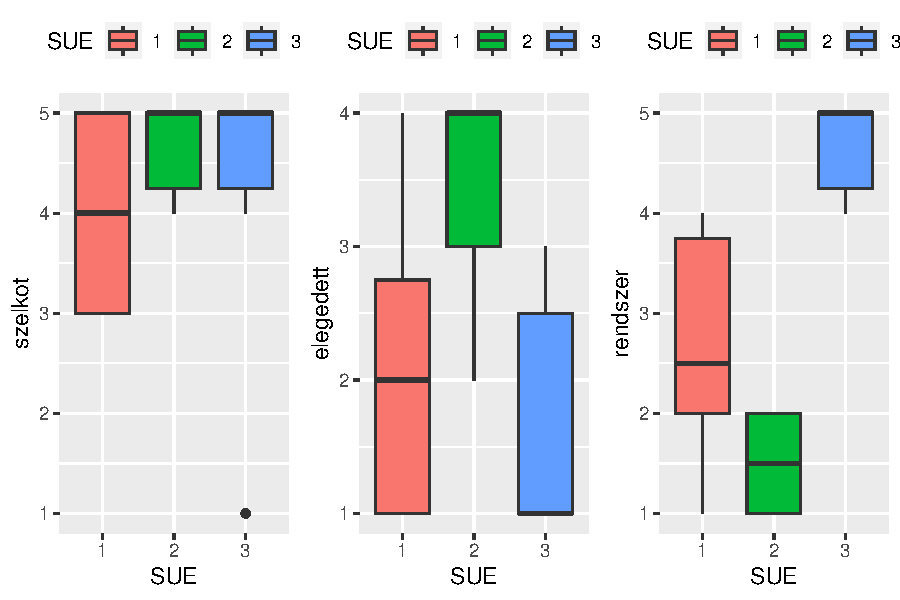
\includegraphics{./sec_tobbvaltozos_variancia_files/figure-pdf/unnamed-chunk-3-1.pdf}

}

\end{figure}

Úgy tűnik, hogy a mindhárom csoport eléggé különbözik egymástól.

Végezzük el az egyszempontos többváltozós variancia elemzést. A
\texttt{manova()} függvény a \texttt{formula=} argumentumában a kettő
vagy több numerikus függő változót és legalább egy független változót
vár. A függő változókat most a \texttt{cbind()} függvénnyel fűztük
egymás mellé, a független változónk pedig a 3 szintű kategorikus
\texttt{SUE}.

\begin{Shaded}
\begin{Highlighting}[]
\NormalTok{man\_1 }\OtherTok{\textless{}{-}} \FunctionTok{manova}\NormalTok{(}\AttributeTok{formula =} \FunctionTok{cbind}\NormalTok{(szelkot, elegedett, rendszer) }\SpecialCharTok{\textasciitilde{}}
\NormalTok{    SUE, }\AttributeTok{data =}\NormalTok{ vezetes)}
\FunctionTok{summary}\NormalTok{(man\_1)}
\CommentTok{\#\textgreater{}           Df  Pillai approx F num Df den Df    Pr(\textgreater{}F)}
\CommentTok{\#\textgreater{} SUE        2 0.90947   7.2278      6     52 1.211e{-}05}
\CommentTok{\#\textgreater{} Residuals 27                                         }
\CommentTok{\#\textgreater{}              }
\CommentTok{\#\textgreater{} SUE       ***}
\CommentTok{\#\textgreater{} Residuals    }
\CommentTok{\#\textgreater{} {-}{-}{-}}
\CommentTok{\#\textgreater{} Signif. codes:  }
\CommentTok{\#\textgreater{} 0 \textquotesingle{}***\textquotesingle{} 0.001 \textquotesingle{}**\textquotesingle{} 0.01 \textquotesingle{}*\textquotesingle{} 0.05 \textquotesingle{}.\textquotesingle{} 0.1 \textquotesingle{} \textquotesingle{} 1}
\end{Highlighting}
\end{Shaded}

Alapértelmezés szerint a MANOVA az R-ben a Pillai-féle
tesztstatisztikáit használja. A p-érték gyakorlatilag nulla, ami azt
jelenti, hogy nyugodtan elvethetjük a nullhipotézist: legalább egy
csoportátlagvektor eltér a többitől.

Használhat más teszteket is, mint például a Wilk-lambda, a Roy-féle vagy
a Hotelling-Lawley statisztikákat, de a Pillai-féle a legrobusztosabb.

\begin{Shaded}
\begin{Highlighting}[]
\FunctionTok{summary}\NormalTok{(man\_1, }\AttributeTok{test =} \StringTok{"Wilks"}\NormalTok{)}
\CommentTok{\#\textgreater{}           Df  Wilks approx F num Df den Df    Pr(\textgreater{}F...}
\CommentTok{\#\textgreater{} SUE        2 0.1894   10.815      6     50 1.102e{-}0...}
\CommentTok{\#\textgreater{} Residuals 27                                       ...}
\CommentTok{\#\textgreater{} {-}{-}{-}}
\CommentTok{\#\textgreater{} Signif. codes:  }
\CommentTok{\#\textgreater{} 0 \textquotesingle{}***\textquotesingle{} 0.001 \textquotesingle{}**\textquotesingle{} 0.01 \textquotesingle{}*\textquotesingle{} 0.05 \textquotesingle{}.\textquotesingle{} 0.1 \textquotesingle{} \textquotesingle{} 1}
\FunctionTok{summary}\NormalTok{(man\_1, }\AttributeTok{test =} \StringTok{"Hotelling{-}Lawley"}\NormalTok{)}
\CommentTok{\#\textgreater{}           Df Hotelling{-}Lawley approx F num Df den Df}
\CommentTok{\#\textgreater{} SUE        2           3.7577   15.031      6     48}
\CommentTok{\#\textgreater{} Residuals 27                                        }
\CommentTok{\#\textgreater{}              Pr(\textgreater{}F)    }
\CommentTok{\#\textgreater{} SUE       1.375e{-}09 ***}
\CommentTok{\#\textgreater{} Residuals              }
\CommentTok{\#\textgreater{} {-}{-}{-}}
\CommentTok{\#\textgreater{} Signif. codes:  }
\CommentTok{\#\textgreater{} 0 \textquotesingle{}***\textquotesingle{} 0.001 \textquotesingle{}**\textquotesingle{} 0.01 \textquotesingle{}*\textquotesingle{} 0.05 \textquotesingle{}.\textquotesingle{} 0.1 \textquotesingle{} \textquotesingle{} 1}
\FunctionTok{summary}\NormalTok{(man\_1, }\AttributeTok{test =} \StringTok{"Roy"}\NormalTok{)}
\CommentTok{\#\textgreater{}           Df    Roy approx F num Df den Df    Pr(\textgreater{}F...}
\CommentTok{\#\textgreater{} SUE        2 3.6133   31.315      3     26 8.724e{-}0...}
\CommentTok{\#\textgreater{} Residuals 27                                       ...}
\CommentTok{\#\textgreater{} {-}{-}{-}}
\CommentTok{\#\textgreater{} Signif. codes:  }
\CommentTok{\#\textgreater{} 0 \textquotesingle{}***\textquotesingle{} 0.001 \textquotesingle{}**\textquotesingle{} 0.01 \textquotesingle{}*\textquotesingle{} 0.05 \textquotesingle{}.\textquotesingle{} 0.1 \textquotesingle{} \textquotesingle{} 1}
\end{Highlighting}
\end{Shaded}

A hatásnagyság kiszámítására MANOVA esetében a parciális Eta négyzet
\((\eta_p^2)\) mutatót használhatjuk. Azt méri, hogy a független változó
milyen hatással van a függő változókra. Ha az érték 0,14 vagy nagyobb,
akkor azt mondhatjuk, hogy a hatás mérete nagy. Ez most 0,45, ami azt
jelenti, hogy a hatás mérete nagy.

\begin{Shaded}
\begin{Highlighting}[]
\NormalTok{effectsize}\SpecialCharTok{::}\FunctionTok{eta\_squared}\NormalTok{(man\_1, }\AttributeTok{partial =}\NormalTok{ T)}
\CommentTok{\#\textgreater{} \# Effect Size for ANOVA (Type I)}
\CommentTok{\#\textgreater{} }
\CommentTok{\#\textgreater{} Parameter | Eta2 (partial) |       95\% CI}
\CommentTok{\#\textgreater{} {-}{-}{-}{-}{-}{-}{-}{-}{-}{-}{-}{-}{-}{-}{-}{-}{-}{-}{-}{-}{-}{-}{-}{-}{-}{-}{-}{-}{-}{-}{-}{-}{-}{-}{-}{-}{-}{-}{-}{-}{-}}
\CommentTok{\#\textgreater{} SUE       |           0.45 | [0.24, 1.00]}
\CommentTok{\#\textgreater{} }
\CommentTok{\#\textgreater{} {-} One{-}sided CIs: upper bound fixed at [1.00].}
\NormalTok{effectsize}\SpecialCharTok{::}\FunctionTok{interpret\_eta\_squared}\NormalTok{(}\FloatTok{0.45}\NormalTok{, }\AttributeTok{partial =}\NormalTok{ T)}
\CommentTok{\#\textgreater{} [1] "large"}
\CommentTok{\#\textgreater{} (Rules: field2013)}
\end{Highlighting}
\end{Shaded}

Mivel a MANOVA szignifikáns lett, további kérdés, hogy melyik csoport
átlagvektora különbözik a többitől? Post-hoc tesztet kell végeznünk,
amely esetünkben a lineáris diszkriminancia elemzés és az egyváltozós
ANOVA lesz.

\hypertarget{post-hoc-teszt-lda}{%
\section{Post-hoc teszt: LDA}\label{post-hoc-teszt-lda}}

A lineáris diszkriminancia elemzés (LDA) célja, hogy változók olyan
lineáris kombinációját találja meg, amely a legjobban elválaszt két vagy
több csoportot. Ezáltal képesek leszünk egy olyan pontdiagramot
megjeleníteni, amely az X és Y tengely két lineáris diszkriminánst
jeleníti meg, a pontokat pedig a független változónak (\texttt{SUE})
megfelelően fogjuk színezni.

A lineáris diszkriminancia elemzést R-ben a \texttt{\{MASS\}} csomag
\texttt{lda()} függvényével végzünk.

\begin{Shaded}
\begin{Highlighting}[]
\FunctionTok{library}\NormalTok{(MASS)}
\NormalTok{lda\_1 }\OtherTok{\textless{}{-}} \FunctionTok{lda}\NormalTok{(SUE }\SpecialCharTok{\textasciitilde{}}\NormalTok{ szelkot }\SpecialCharTok{+}\NormalTok{ elegedett }\SpecialCharTok{+}\NormalTok{ rendszer, }\AttributeTok{data =}\NormalTok{ vezetes)}
\NormalTok{lda\_1}
\CommentTok{\#\textgreater{} Call:}
\CommentTok{\#\textgreater{} lda(SUE \textasciitilde{} szelkot + elegedett + rendszer, data = ve...}
\CommentTok{\#\textgreater{} }
\CommentTok{\#\textgreater{} Prior probabilities of groups:}
\CommentTok{\#\textgreater{}         1         2         3 }
\CommentTok{\#\textgreater{} 0.3333333 0.3333333 0.3333333 }
\CommentTok{\#\textgreater{} }
\CommentTok{\#\textgreater{} Group means:}
\CommentTok{\#\textgreater{}   szelkot elegedett rendszer}
\CommentTok{\#\textgreater{} 1     4.0       2.1      2.7}
\CommentTok{\#\textgreater{} 2     4.7       3.4      1.5}
\CommentTok{\#\textgreater{} 3     4.1       1.6      4.7}
\CommentTok{\#\textgreater{} }
\CommentTok{\#\textgreater{} Coefficients of linear discriminants:}
\CommentTok{\#\textgreater{}                   LD1       LD2}
\CommentTok{\#\textgreater{} szelkot   {-}0.07056752 0.4959142}
\CommentTok{\#\textgreater{} elegedett  0.10193972 0.8596451}
\CommentTok{\#\textgreater{} rendszer  {-}1.32360357 0.5392379}
\CommentTok{\#\textgreater{} }
\CommentTok{\#\textgreater{} Proportion of trace:}
\CommentTok{\#\textgreater{}    LD1    LD2 }
\CommentTok{\#\textgreater{} 0.9616 0.0384}
\CommentTok{\# klaR::greedy.wilks(vasarlas\textasciitilde{}ertek+attitud+fizetes+kor,data=bio,}
\CommentTok{\# niveau = 0.15)}
\end{Highlighting}
\end{Shaded}

A fenti együtthatókból megtudhatjuk hogyan használják fel a függő
változókat az LDA döntési szabályának kialakítására. Az LD1 a
következőképpen számítható ki:

A \texttt{vezetes} adatmátrix numerikus változóira magunk is
kiszámolhatjuk az LD1 és LDA2 értékét a \texttt{predict()} függvénnyel:

\begin{Shaded}
\begin{Highlighting}[]
\NormalTok{lda\_1\_pred }\OtherTok{\textless{}{-}} \FunctionTok{predict}\NormalTok{(lda\_1, }\AttributeTok{method =} \StringTok{"plug{-}in"}\NormalTok{)}
\NormalTok{psych}\SpecialCharTok{::}\FunctionTok{headTail}\NormalTok{(lda\_1\_pred}\SpecialCharTok{$}\NormalTok{x)}
\CommentTok{\#\textgreater{}       LD1   LD2}
\CommentTok{\#\textgreater{} 1    1.16 {-}1.83}
\CommentTok{\#\textgreater{} 2    2.69 {-}0.65}
\CommentTok{\#\textgreater{} 3    1.39  1.25}
\CommentTok{\#\textgreater{} 4   {-}1.56 {-}0.25}
\CommentTok{\#\textgreater{} ...   ...   ...}
\CommentTok{\#\textgreater{} 27   {-}2.6  {-}1.7}
\CommentTok{\#\textgreater{} 28  {-}1.56 {-}0.25}
\CommentTok{\#\textgreater{} 29  {-}2.88  0.29}
\CommentTok{\#\textgreater{} 30  {-}1.35  1.47}
\end{Highlighting}
\end{Shaded}

A post-hoc teszt utolsó lépése a fenti a pontdiagram megjelenítése.
Ideális esetben egy vagy több csoport kiemelkedik:

\begin{Shaded}
\begin{Highlighting}[]
\NormalTok{d }\OtherTok{\textless{}{-}} \FunctionTok{data.frame}\NormalTok{(lda\_1\_pred}\SpecialCharTok{$}\NormalTok{x, }\AttributeTok{SUE =}\NormalTok{ vezetes}\SpecialCharTok{$}\NormalTok{SUE)}
\NormalTok{psych}\SpecialCharTok{::}\FunctionTok{headTail}\NormalTok{(d)}
\CommentTok{\#\textgreater{}       LD1   LD2  SUE}
\CommentTok{\#\textgreater{} 1    1.16 {-}1.83    1}
\CommentTok{\#\textgreater{} 2    2.69 {-}0.65    1}
\CommentTok{\#\textgreater{} 3    1.39  1.25    1}
\CommentTok{\#\textgreater{} 4   {-}1.56 {-}0.25    1}
\CommentTok{\#\textgreater{} ...   ...   ... \textless{}NA\textgreater{}}
\CommentTok{\#\textgreater{} 27   {-}2.6  {-}1.7    3}
\CommentTok{\#\textgreater{} 28  {-}1.56 {-}0.25    3}
\CommentTok{\#\textgreater{} 29  {-}2.88  0.29    3}
\CommentTok{\#\textgreater{} 30  {-}1.35  1.47    3}
\end{Highlighting}
\end{Shaded}

\begin{Shaded}
\begin{Highlighting}[]
\FunctionTok{ggplot}\NormalTok{(d, }\FunctionTok{aes}\NormalTok{(}\AttributeTok{x =}\NormalTok{ LD1, }\AttributeTok{y =}\NormalTok{ LD2, }\AttributeTok{colour =}\NormalTok{ SUE)) }\SpecialCharTok{+} \FunctionTok{geom\_point}\NormalTok{(}\AttributeTok{size =} \DecValTok{4}\NormalTok{)}
\end{Highlighting}
\end{Shaded}

\begin{figure}[H]

{\centering 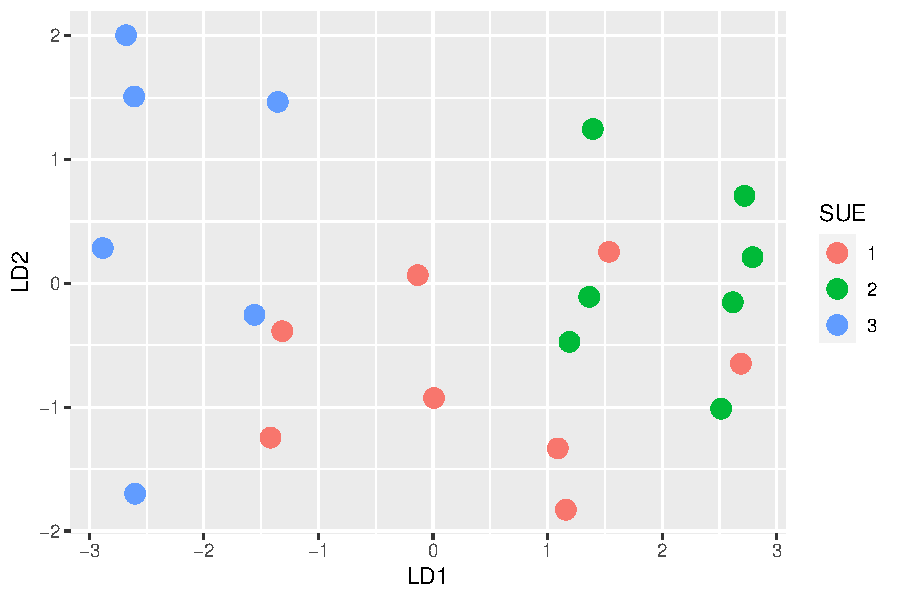
\includegraphics{./sec_tobbvaltozos_variancia_files/figure-pdf/unnamed-chunk-10-1.pdf}

}

\end{figure}

A képen látható, hogy a harmadik SÜE csoport eltér mindkét másik
csoporttól, míg a az első két csoport eltérése egymástól nem mondható
markánsnak. Könnyen elképzelhető, hogy a SÜE harmadik csoportja volt a
legnagyobb hatással a nullhipotézis elutasítására.

\hypertarget{post-hoc-test-egyvuxe1ltozuxf3s-vizsguxe1latok}{%
\section{Post-hoc test: egyváltozós
vizsgálatok}\label{post-hoc-test-egyvuxe1ltozuxf3s-vizsguxe1latok}}

A statisztikailag szignifikáns egyszempontos MANOVA után az egyváltozós
egyszempontos ANOVA-val is vizsgálódhatunk, amely minden függő változót
külön-külön vizsgál. A cél az, hogy azonosítsuk azokat a konkrét függő
változókat, amelyek hozzájárultak a jelentős globális hatáshoz. A
klasszikus ANOVA mellett a Welch-féle változat és a
Kruskal--Wallis-próba is használható, a feltételek egyre nagyobb
csorbulása esetén. Most a nemparaméteres Kruskal--Wallis-próbát
használjuk.

\begin{Shaded}
\begin{Highlighting}[]
\FunctionTok{kruskal.test}\NormalTok{(szelkot }\SpecialCharTok{\textasciitilde{}}\NormalTok{ SUE, }\AttributeTok{data =}\NormalTok{ vezetes)}\SpecialCharTok{$}\NormalTok{p.value}
\CommentTok{\#\textgreater{} [1] 0.2499069}
\FunctionTok{kruskal.test}\NormalTok{(elegedett }\SpecialCharTok{\textasciitilde{}}\NormalTok{ SUE, }\AttributeTok{data =}\NormalTok{ vezetes)}\SpecialCharTok{$}\NormalTok{p.value}
\CommentTok{\#\textgreater{} [1] 0.003003241}
\FunctionTok{kruskal.test}\NormalTok{(rendszer }\SpecialCharTok{\textasciitilde{}}\NormalTok{ SUE, }\AttributeTok{data =}\NormalTok{ vezetes)}\SpecialCharTok{$}\NormalTok{p.value}
\CommentTok{\#\textgreater{} [1] 1.690362e{-}05}
\end{Highlighting}
\end{Shaded}

Látjuk, hogy az \texttt{elegedett} és a \texttt{rendszer} függő
változókban nem egyeznek a várható értékek a SÜE egyes csoportjaiban.
Megjegyezzük, hogy mivel 3 függő változónk van, a Bonferroni-féle
többszörös tesztelési korrekciót alkalmaznunk kell, vagyis a
statisztikai szignifikancia szintet csökkenteni kell. Ez úgy történik,
hogy a klasszikus alfa szintet (0,05) elosztjuk a tesztek (vagy függő
változók, itt 3) számával. Ez p \textless{} 0,017-es szignifikancia
elfogadási kritériumhoz vezet. A fenti próbák szignifikáns voltán ez
most nem változtat.

A statisztikailag szignifikáns egyváltozós ANOVA-t (esetünkben
Kruskal--Wallis-próbát) többszörös páronkénti összehasonlítás követi
annak meghatározására, hogy mely csoportok különböznek egymástól. Most a
Kruskal--Wallis-próba szokásos utóvizsgálatát a Dunn-próbát fogjuk
használni.

\begin{Shaded}
\begin{Highlighting}[]
\FunctionTok{library}\NormalTok{(DescTools)}
\FunctionTok{DunnTest}\NormalTok{(}\AttributeTok{formula =}\NormalTok{ szelkot }\SpecialCharTok{\textasciitilde{}}\NormalTok{ SUE, }\AttributeTok{data =}\NormalTok{ vezetes, }\AttributeTok{method =} \StringTok{"holm"}\NormalTok{)}
\CommentTok{\#\textgreater{} }
\CommentTok{\#\textgreater{}  Dunn\textquotesingle{}s test of multiple comparisons using rank sum...}
\CommentTok{\#\textgreater{} }
\CommentTok{\#\textgreater{}     mean.rank.diff   pval    }
\CommentTok{\#\textgreater{} 2{-}1            5.6 0.3179    }
\CommentTok{\#\textgreater{} 3{-}1            4.0 0.4964    }
\CommentTok{\#\textgreater{} 3{-}2           {-}1.6 0.6442    }
\CommentTok{\#\textgreater{} {-}{-}{-}}
\CommentTok{\#\textgreater{} Signif. codes:  0 \textquotesingle{}***\textquotesingle{} 0.001 \textquotesingle{}**\textquotesingle{} 0.01 \textquotesingle{}*\textquotesingle{} 0.05 \textquotesingle{}....}
\FunctionTok{DunnTest}\NormalTok{(}\AttributeTok{formula =}\NormalTok{ elegedett }\SpecialCharTok{\textasciitilde{}}\NormalTok{ SUE, }\AttributeTok{data =}\NormalTok{ vezetes, }\AttributeTok{method =} \StringTok{"holm"}\NormalTok{)}
\CommentTok{\#\textgreater{} }
\CommentTok{\#\textgreater{}  Dunn\textquotesingle{}s test of multiple comparisons using rank sum...}
\CommentTok{\#\textgreater{} }
\CommentTok{\#\textgreater{}     mean.rank.diff   pval    }
\CommentTok{\#\textgreater{} 2{-}1           8.75 0.0410 *  }
\CommentTok{\#\textgreater{} 3{-}1          {-}3.80 0.3143    }
\CommentTok{\#\textgreater{} 3{-}2         {-}12.55 0.0027 ** }
\CommentTok{\#\textgreater{} {-}{-}{-}}
\CommentTok{\#\textgreater{} Signif. codes:  0 \textquotesingle{}***\textquotesingle{} 0.001 \textquotesingle{}**\textquotesingle{} 0.01 \textquotesingle{}*\textquotesingle{} 0.05 \textquotesingle{}....}
\FunctionTok{DunnTest}\NormalTok{(}\AttributeTok{formula =}\NormalTok{ rendszer }\SpecialCharTok{\textasciitilde{}}\NormalTok{ SUE, }\AttributeTok{data =}\NormalTok{ vezetes, }\AttributeTok{method =} \StringTok{"holm"}\NormalTok{)}
\CommentTok{\#\textgreater{} }
\CommentTok{\#\textgreater{}  Dunn\textquotesingle{}s test of multiple comparisons using rank sum...}
\CommentTok{\#\textgreater{} }
\CommentTok{\#\textgreater{}     mean.rank.diff    pval    }
\CommentTok{\#\textgreater{} 2{-}1          {-}6.95  0.0694 .  }
\CommentTok{\#\textgreater{} 3{-}1          10.85  0.0092 ** }
\CommentTok{\#\textgreater{} 3{-}2          17.80 9.9e{-}06 ***}
\CommentTok{\#\textgreater{} {-}{-}{-}}
\CommentTok{\#\textgreater{} Signif. codes:  0 \textquotesingle{}***\textquotesingle{} 0.001 \textquotesingle{}**\textquotesingle{} 0.01 \textquotesingle{}*\textquotesingle{} 0.05 \textquotesingle{}....}
\end{Highlighting}
\end{Shaded}

A fenti utóvizsgálatok világossá teszik, hogy a harmadik SÜE csoport a
\texttt{rendszer} változó esetén mindkét másik csoporttól, az
\texttt{elegedett} változó esetén pedig a második csoporttól
szignifikánsan eltér. Legjelentősebb mértékben tehűt a harmadik csoport
különül el a másik két csoporttól, tehát ez okozza a MANOVA
nullhipotézisének elvetését.

\hypertarget{elemzuxe9s-jamovi-ban}{%
\section{Elemzés jamovi-ban}\label{elemzuxe9s-jamovi-ban}}

A fenti elemzés jamovi-ban is elvégezhető az \texttt{ANOVA\ /\ MANCOVA}
menüpontok kiválasztásával.

\begin{figure}

{\centering 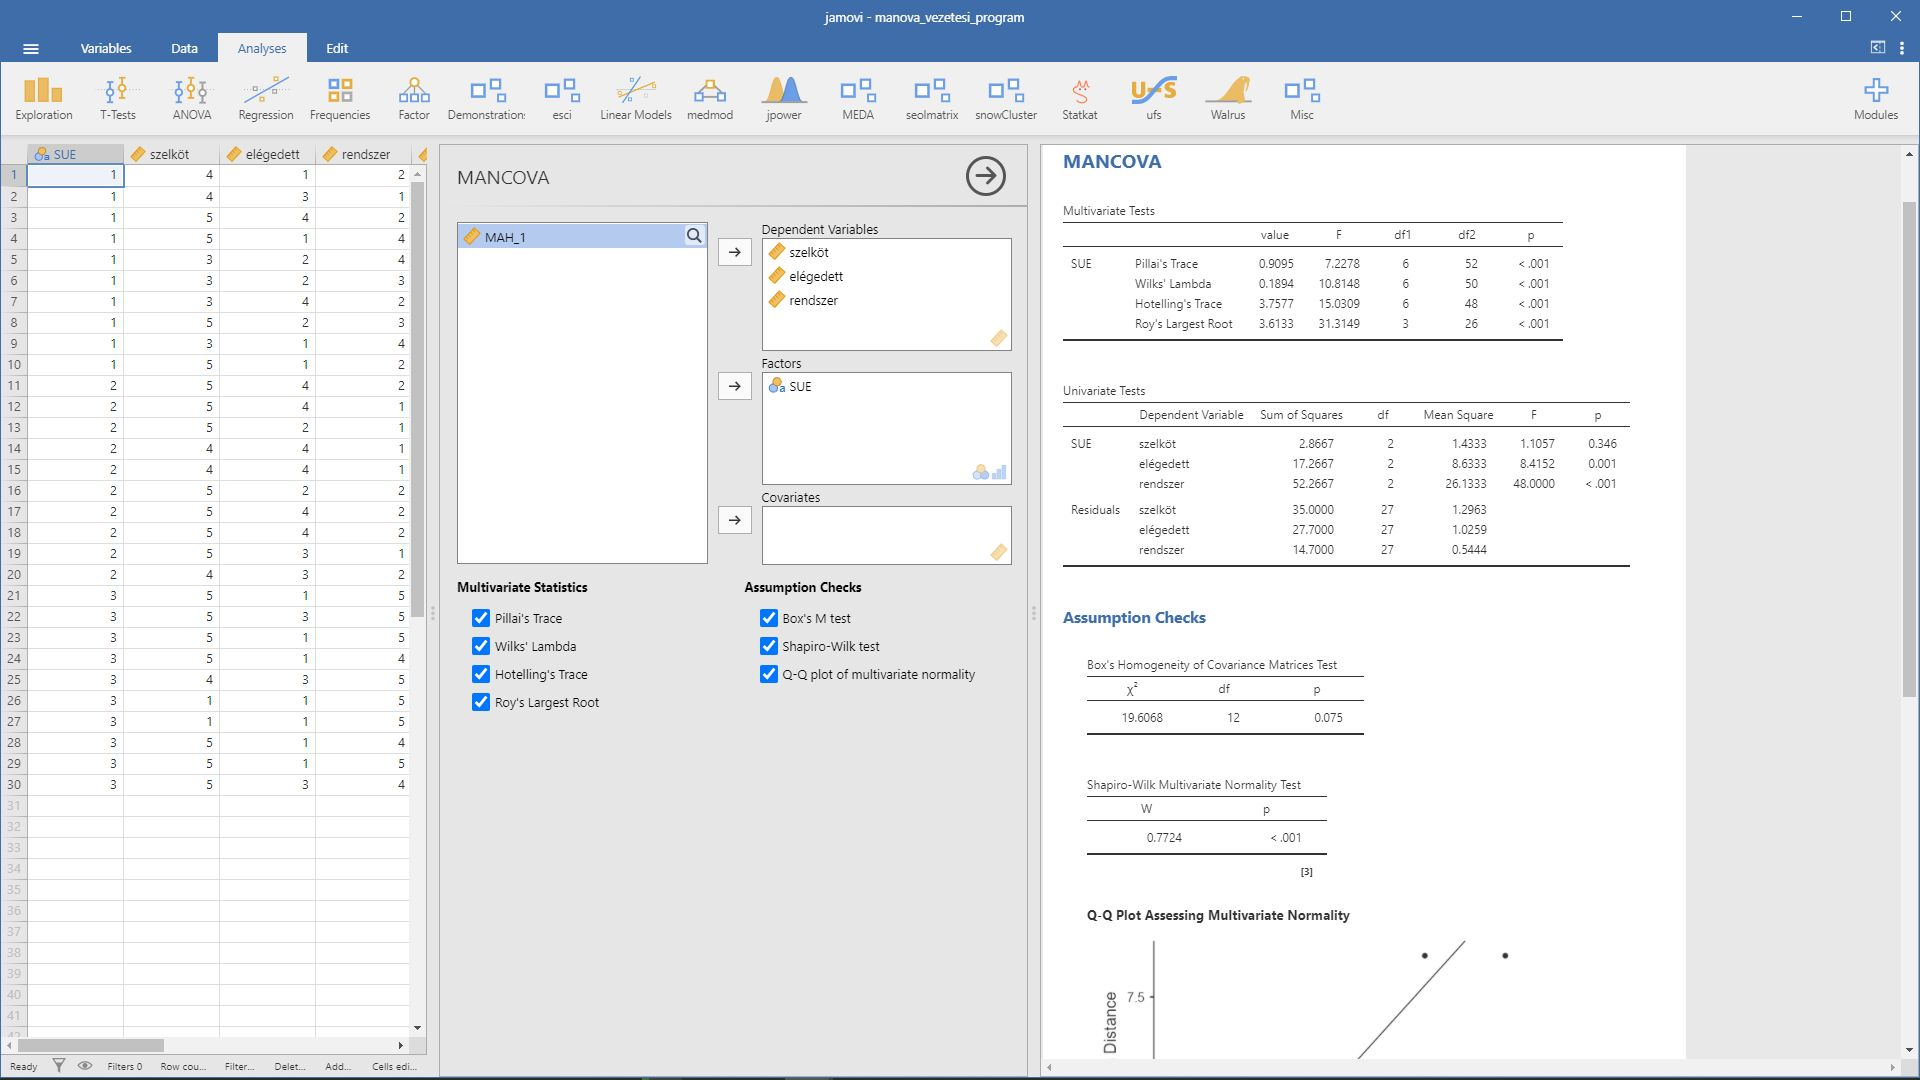
\includegraphics{./images/manova_kep_01.jpg}

}

\caption{MANOVA jamovi-ban}

\end{figure}

\hypertarget{alkalmazuxe1si-feltuxe9telek-vizsguxe1lata}{%
\section{Alkalmazási feltételek
vizsgálata}\label{alkalmazuxe1si-feltuxe9telek-vizsguxe1lata}}

A MANOVA statisztikai próbának számos szigorú alkalmazási feltétele van.
Néhány az ANOVA-ból jön, például a megfigyelések függetlensége vagy a
variancia homogenitása, azonban vannak újdonságok is.

\begin{itemize}
\tightlist
\item
  \textbf{Megfelelő mintanagyság.} Ökölszabály: a mintaelemszám
  mindegyik független változó csoportban nagyobb az függő változók
  számánál.
\end{itemize}

\begin{Shaded}
\begin{Highlighting}[]
\NormalTok{summarytools}\SpecialCharTok{::}\FunctionTok{freq}\NormalTok{(vezetes}\SpecialCharTok{$}\NormalTok{SUE, }\AttributeTok{cumul =} \ConstantTok{FALSE}\NormalTok{)}
\CommentTok{\#\textgreater{} Frequencies  }
\CommentTok{\#\textgreater{} vezetes$SUE  }
\CommentTok{\#\textgreater{} Type: Factor  }
\CommentTok{\#\textgreater{} }
\CommentTok{\#\textgreater{}               Freq   \% Valid   \% Total}
\CommentTok{\#\textgreater{} {-}{-}{-}{-}{-}{-}{-}{-}{-}{-}{-} {-}{-}{-}{-}{-}{-} {-}{-}{-}{-}{-}{-}{-}{-}{-} {-}{-}{-}{-}{-}{-}{-}{-}{-}}
\CommentTok{\#\textgreater{}           1     10     33.33     33.33}
\CommentTok{\#\textgreater{}           2     10     33.33     33.33}
\CommentTok{\#\textgreater{}           3     10     33.33     33.33}
\CommentTok{\#\textgreater{}        \textless{}NA\textgreater{}      0                0.00}
\CommentTok{\#\textgreater{}       Total     30    100.00    100.00}
\end{Highlighting}
\end{Shaded}

Látható, hogy a függő változók számát (3) minden csoport elemszáma (10)
meghaladja.

\begin{itemize}
\item
  \textbf{A megfigyelések függetlensége.} Minden személynek csak egy
  csoportba kell tartoznia. Az egyes csoportok megfigyelései között
  nincs kapcsolat. Az ismételt mérések nem megengedettek. A minta
  kiválasztásának teljesen véletlenszerűnek kell lennie.
\item
  \textbf{Az egyváltozós vagy többváltozós kiugró értékek hiánya.}
\end{itemize}

Az egydimenziós kiugró értékek dobozdiagramokkal is ellenőrizhetők, ezt
korábban elvégeztük, láttuk csak egyetlen részcsoportban van kiugró
értékek (a \texttt{szelkot} változó változó esetén a SÜE harmadik
csoportjában). Használhatjuk a kényelmes
\texttt{rstatix::identify\_outliers()} függvényt is.

\begin{Shaded}
\begin{Highlighting}[]
\FunctionTok{library}\NormalTok{(tidyverse)}
\NormalTok{vezetes }\SpecialCharTok{\%\textgreater{}\%}
    \FunctionTok{group\_by}\NormalTok{(SUE) }\SpecialCharTok{\%\textgreater{}\%}
\NormalTok{    rstatix}\SpecialCharTok{::}\FunctionTok{identify\_outliers}\NormalTok{(szelkot)}
\CommentTok{\#\textgreater{} \# A tibble: 2 x 6}
\CommentTok{\#\textgreater{}   SUE   szelkot elegedett rendszer is.outlier is.ex...}
\CommentTok{\#\textgreater{}   \textless{}fct\textgreater{}   \textless{}dbl\textgreater{}     \textless{}dbl\textgreater{}    \textless{}dbl\textgreater{} \textless{}lgl\textgreater{}      \textless{}lgl\textgreater{}...}
\CommentTok{\#\textgreater{} 1 3           1         1        5 TRUE       TRUE ...}
\CommentTok{\#\textgreater{} 2 3           1         1        5 TRUE       TRUE}
\NormalTok{vezetes }\SpecialCharTok{\%\textgreater{}\%}
    \FunctionTok{group\_by}\NormalTok{(SUE) }\SpecialCharTok{\%\textgreater{}\%}
\NormalTok{    rstatix}\SpecialCharTok{::}\FunctionTok{identify\_outliers}\NormalTok{(elegedett)}
\CommentTok{\#\textgreater{} [1] SUE        szelkot    elegedett  rendszer  }
\CommentTok{\#\textgreater{} [5] is.outlier is.extreme}
\CommentTok{\#\textgreater{} \textless{}0 rows\textgreater{} (or 0{-}length row.names)}
\NormalTok{vezetes }\SpecialCharTok{\%\textgreater{}\%}
    \FunctionTok{group\_by}\NormalTok{(SUE) }\SpecialCharTok{\%\textgreater{}\%}
\NormalTok{    rstatix}\SpecialCharTok{::}\FunctionTok{identify\_outliers}\NormalTok{(rendszer)}
\CommentTok{\#\textgreater{} [1] SUE        szelkot    elegedett  rendszer  }
\CommentTok{\#\textgreater{} [5] is.outlier is.extreme}
\CommentTok{\#\textgreater{} \textless{}0 rows\textgreater{} (or 0{-}length row.names)}
\end{Highlighting}
\end{Shaded}

A többváltozós kiugró értékek olyan adatpontok, amelyek szokatlan
értékkombinációt tartalmaznak a kimeneti (vagy függő) változókon. A
Mahalanobis távolságot általában a többváltozós kiugró értékek
észlelésére használják. A távolság megmondja, milyen messze van egy
megfigyelés a felhő középpontjától, figyelembe véve a felhő alakját
(kovariancia) is. A \texttt{rstatix::mahalanobis\_distance()} függvény
könnyen használható a Mahalanobis-távolság kiszámítására és a
többváltozós kiugró értékek megjelölésére. A Mahalanobis-távolságot
csoportonként kell kiszámítani:

\begin{Shaded}
\begin{Highlighting}[]
\NormalTok{vezetes }\SpecialCharTok{\%\textgreater{}\%}
    \FunctionTok{group\_by}\NormalTok{(SUE) }\SpecialCharTok{\%\textgreater{}\%}
\NormalTok{    rstatix}\SpecialCharTok{::}\FunctionTok{mahalanobis\_distance}\NormalTok{() }\SpecialCharTok{\%\textgreater{}\%}
    \FunctionTok{filter}\NormalTok{(is.outlier }\SpecialCharTok{==} \ConstantTok{TRUE}\NormalTok{) }\SpecialCharTok{\%\textgreater{}\%}
    \FunctionTok{as.data.frame}\NormalTok{()}
\CommentTok{\#\textgreater{} [1] szelkot    elegedett  rendszer   mahal.dist}
\CommentTok{\#\textgreater{} [5] is.outlier}
\CommentTok{\#\textgreater{} \textless{}0 rows\textgreater{} (or 0{-}length row.names)}
\end{Highlighting}
\end{Shaded}

Látható, hogy nincs többváltozós kiugró érték az adatbázisban.

\begin{itemize}
\tightlist
\item
  \textbf{Többváltozós normalitás.}
\end{itemize}

A többváltozós normalitás Shapiro-Wilk tesztjének végrehajtása:

\begin{Shaded}
\begin{Highlighting}[]
\NormalTok{rstatix}\SpecialCharTok{::}\FunctionTok{mshapiro\_test}\NormalTok{(vezetes[}\FunctionTok{c}\NormalTok{(}\StringTok{"szelkot"}\NormalTok{, }\StringTok{"elegedett"}\NormalTok{, }\StringTok{"rendszer"}\NormalTok{)])}
\CommentTok{\#\textgreater{} \# A tibble: 1 x 2}
\CommentTok{\#\textgreater{}   statistic   p.value}
\CommentTok{\#\textgreater{}       \textless{}dbl\textgreater{}     \textless{}dbl\textgreater{}}
\CommentTok{\#\textgreater{} 1     0.772 0.0000214}
\end{Highlighting}
\end{Shaded}

Látható, hogy ez az alkalmazási feltétel nem teljesül.

Az egyváltozós normalitásokat is érdemes lehet tesztelni:

\begin{Shaded}
\begin{Highlighting}[]
\CommentTok{\# egyváltozós Shapiro–Wilk próba több csoportra}
\FunctionTok{library}\NormalTok{(onewaytests)}
\FunctionTok{nor.test}\NormalTok{(}\AttributeTok{formula =}\NormalTok{ szelkot }\SpecialCharTok{\textasciitilde{}}\NormalTok{ SUE, }\AttributeTok{data =}\NormalTok{ vezetes, }\AttributeTok{method =} \StringTok{"SW"}\NormalTok{)}
\CommentTok{\#\textgreater{} }
\CommentTok{\#\textgreater{}   Shapiro{-}Wilk Normality Test (alpha = 0.05) }
\CommentTok{\#\textgreater{} {-}{-}{-}{-}{-}{-}{-}{-}{-}{-}{-}{-}{-}{-}{-}{-}{-}{-}{-}{-}{-}{-}{-}{-}{-}{-}{-}{-}{-}{-}{-}{-}{-}{-}{-}{-}{-}{-}{-}{-}{-}{-}{-}{-}{-}{-}{-}{-}{-}{-} }
\CommentTok{\#\textgreater{}   data : szelkot and SUE }
\CommentTok{\#\textgreater{} }
\CommentTok{\#\textgreater{}   Level Statistic      p.value   Normality}
\CommentTok{\#\textgreater{} 1     1 0.7685823 6.009970e{-}03      Reject}
\CommentTok{\#\textgreater{} 2     2 0.5941735 4.713464e{-}05      Reject}
\CommentTok{\#\textgreater{} 3     3 0.5876023 3.936679e{-}05      Reject}
\CommentTok{\#\textgreater{} {-}{-}{-}{-}{-}{-}{-}{-}{-}{-}{-}{-}{-}{-}{-}{-}{-}{-}{-}{-}{-}{-}{-}{-}{-}{-}{-}{-}{-}{-}{-}{-}{-}{-}{-}{-}{-}{-}{-}{-}{-}{-}{-}{-}{-}{-}{-}{-}{-}{-}}
\FunctionTok{nor.test}\NormalTok{(}\AttributeTok{formula =}\NormalTok{ elegedett }\SpecialCharTok{\textasciitilde{}}\NormalTok{ SUE, }\AttributeTok{data =}\NormalTok{ vezetes, }\AttributeTok{method =} \StringTok{"SW"}\NormalTok{)}
\CommentTok{\#\textgreater{} }
\CommentTok{\#\textgreater{}   Shapiro{-}Wilk Normality Test (alpha = 0.05) }
\CommentTok{\#\textgreater{} {-}{-}{-}{-}{-}{-}{-}{-}{-}{-}{-}{-}{-}{-}{-}{-}{-}{-}{-}{-}{-}{-}{-}{-}{-}{-}{-}{-}{-}{-}{-}{-}{-}{-}{-}{-}{-}{-}{-}{-}{-}{-}{-}{-}{-}{-}{-}{-}{-}{-} }
\CommentTok{\#\textgreater{}   data : elegedett and SUE }
\CommentTok{\#\textgreater{} }
\CommentTok{\#\textgreater{}   Level Statistic      p.value   Normality}
\CommentTok{\#\textgreater{} 1     1 0.8236140 2.802300e{-}02      Reject}
\CommentTok{\#\textgreater{} 2     2 0.7172415 1.425861e{-}03      Reject}
\CommentTok{\#\textgreater{} 3     3 0.5941735 4.713464e{-}05      Reject}
\CommentTok{\#\textgreater{} {-}{-}{-}{-}{-}{-}{-}{-}{-}{-}{-}{-}{-}{-}{-}{-}{-}{-}{-}{-}{-}{-}{-}{-}{-}{-}{-}{-}{-}{-}{-}{-}{-}{-}{-}{-}{-}{-}{-}{-}{-}{-}{-}{-}{-}{-}{-}{-}{-}{-}}
\FunctionTok{nor.test}\NormalTok{(}\AttributeTok{formula =}\NormalTok{ rendszer }\SpecialCharTok{\textasciitilde{}}\NormalTok{ SUE, }\AttributeTok{data =}\NormalTok{ vezetes, }\AttributeTok{method =} \StringTok{"SW"}\NormalTok{)}
\CommentTok{\#\textgreater{} }
\CommentTok{\#\textgreater{}   Shapiro{-}Wilk Normality Test (alpha = 0.05) }
\CommentTok{\#\textgreater{} {-}{-}{-}{-}{-}{-}{-}{-}{-}{-}{-}{-}{-}{-}{-}{-}{-}{-}{-}{-}{-}{-}{-}{-}{-}{-}{-}{-}{-}{-}{-}{-}{-}{-}{-}{-}{-}{-}{-}{-}{-}{-}{-}{-}{-}{-}{-}{-}{-}{-} }
\CommentTok{\#\textgreater{}   data : rendszer and SUE }
\CommentTok{\#\textgreater{} }
\CommentTok{\#\textgreater{}   Level Statistic      p.value   Normality}
\CommentTok{\#\textgreater{} 1     1 0.8737456 1.105101e{-}01  Not reject}
\CommentTok{\#\textgreater{} 2     2 0.6552710 2.539627e{-}04      Reject}
\CommentTok{\#\textgreater{} 3     3 0.5941735 4.713464e{-}05      Reject}
\CommentTok{\#\textgreater{} {-}{-}{-}{-}{-}{-}{-}{-}{-}{-}{-}{-}{-}{-}{-}{-}{-}{-}{-}{-}{-}{-}{-}{-}{-}{-}{-}{-}{-}{-}{-}{-}{-}{-}{-}{-}{-}{-}{-}{-}{-}{-}{-}{-}{-}{-}{-}{-}{-}{-}}
\end{Highlighting}
\end{Shaded}

\begin{figure}[H]

{\centering 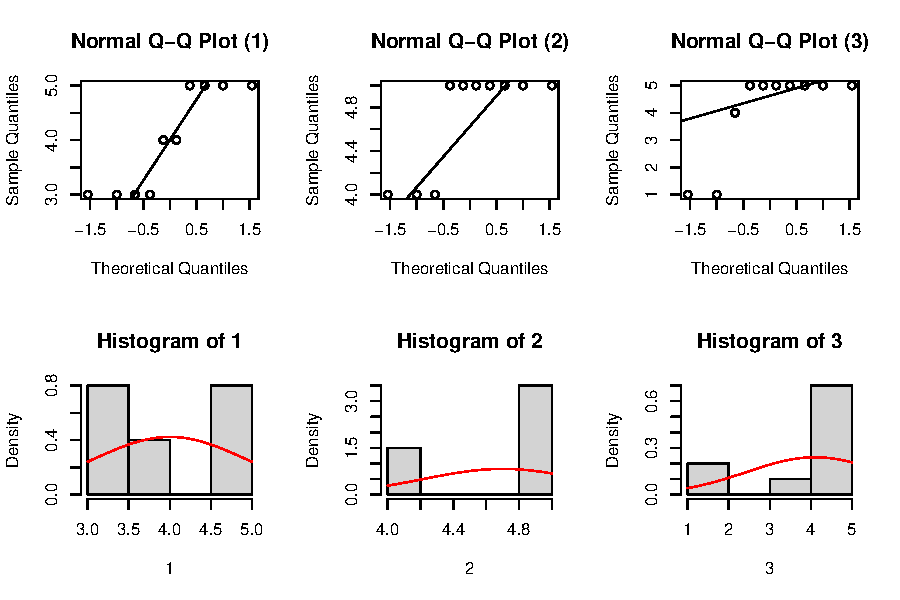
\includegraphics{./sec_tobbvaltozos_variancia_files/figure-pdf/unnamed-chunk-17-1.pdf}

}

\end{figure}

\begin{figure}[H]

{\centering 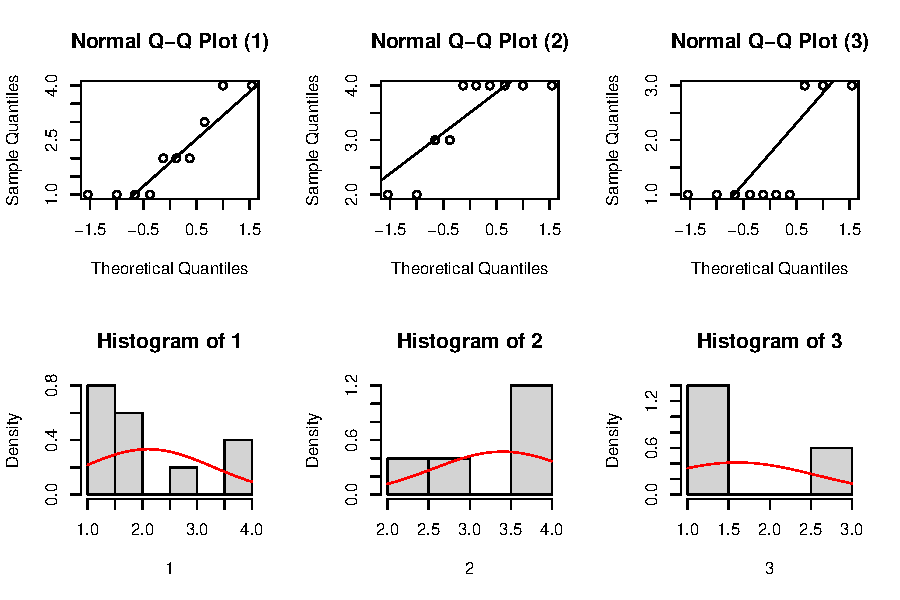
\includegraphics{./sec_tobbvaltozos_variancia_files/figure-pdf/unnamed-chunk-17-2.pdf}

}

\end{figure}

\begin{figure}[H]

{\centering 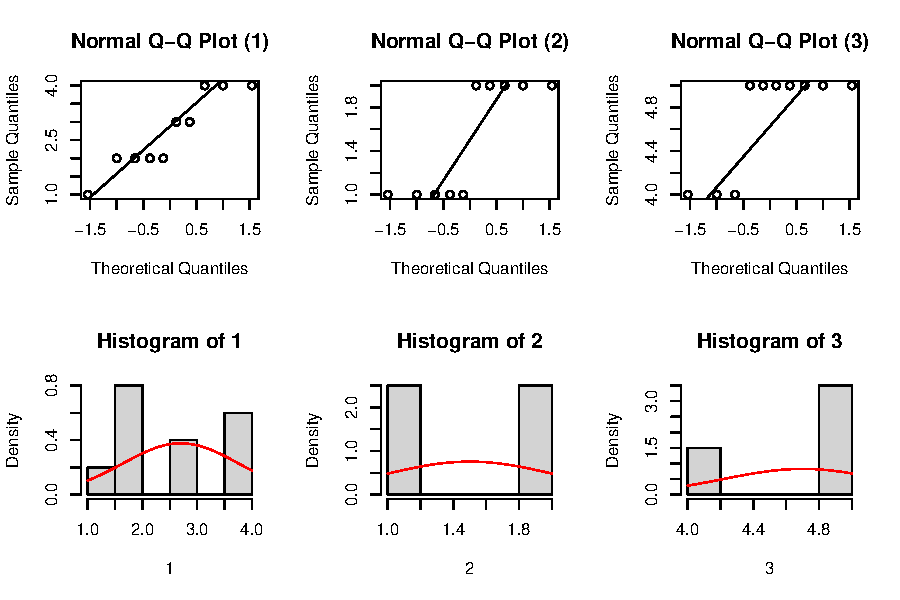
\includegraphics{./sec_tobbvaltozos_variancia_files/figure-pdf/unnamed-chunk-17-3.pdf}

}

\end{figure}

\begin{itemize}
\tightlist
\item
  \textbf{A multikollinearitás hiánya.} A függő (eredmény) változók nem
  korrelálhatnak túlságosan egymással. Egyetlen korreláció sem lehet r =
  0,90 feletti.
\end{itemize}

Ideális esetben az eredményváltozók közötti korreláció mérsékelt, nem
túl magas. A 0,9 feletti korreláció a multikollinearitást jelzi, ami a
MANOVA esetében problematikus. Másrészt, ha a korreláció túl alacsony,
fontolóra kell vennie külön egyszempontos ANOVA futtatását minden függő
változóra.

Számítsuk ki a páronkénti Pearson-korrelációs együtthatókat a függő
változók között.

\begin{Shaded}
\begin{Highlighting}[]
\FunctionTok{cor}\NormalTok{(vezetes[}\FunctionTok{c}\NormalTok{(}\StringTok{"szelkot"}\NormalTok{, }\StringTok{"elegedett"}\NormalTok{, }\StringTok{"rendszer"}\NormalTok{)])}
\CommentTok{\#\textgreater{}              szelkot  elegedett   rendszer}
\CommentTok{\#\textgreater{} szelkot    1.0000000  0.1954881 {-}0.2528624}
\CommentTok{\#\textgreater{} elegedett  0.1954881  1.0000000 {-}0.6129079}
\CommentTok{\#\textgreater{} rendszer  {-}0.2528624 {-}0.6129079  1.0000000}
\end{Highlighting}
\end{Shaded}

Látható, hogy a korrelációs együtthatók nem támogatják a
multikollinearitás tényét.

\begin{itemize}
\tightlist
\item
  \textbf{Linearitás az összes függő változó között minden csoportban.}
\end{itemize}

Mivel a függő változók közötti páronkénti kapcsolatnak lineárisnak kell
lennie minden csoport esetében, ezért érdemes ezt a feltételt vizuálisan
ellenőrizni. A \texttt{\{GGally\}} csomag \texttt{ggpairs()} függvényét
használhatjuk.

\begin{Shaded}
\begin{Highlighting}[]
\FunctionTok{library}\NormalTok{(GGally)}
\NormalTok{res }\OtherTok{\textless{}{-}}\NormalTok{ vezetes }\SpecialCharTok{\%\textgreater{}\%}
    \FunctionTok{select}\NormalTok{(SUE, szelkot, elegedett, rendszer) }\SpecialCharTok{\%\textgreater{}\%}
    \FunctionTok{group\_by}\NormalTok{(SUE) }\SpecialCharTok{\%\textgreater{}\%}
\NormalTok{    rstatix}\SpecialCharTok{::}\FunctionTok{doo}\NormalTok{(}\SpecialCharTok{\textasciitilde{}}\FunctionTok{ggpairs}\NormalTok{(.) }\SpecialCharTok{+} \FunctionTok{theme\_bw}\NormalTok{(), }\AttributeTok{result =} \StringTok{"plots"}\NormalTok{)}
\NormalTok{res}\SpecialCharTok{$}\NormalTok{plots}
\CommentTok{\#\textgreater{} [[1]]}
\CommentTok{\#\textgreater{} }
\CommentTok{\#\textgreater{} [[2]]}
\CommentTok{\#\textgreater{} }
\CommentTok{\#\textgreater{} [[3]]}
\end{Highlighting}
\end{Shaded}

\begin{figure}[H]

{\centering 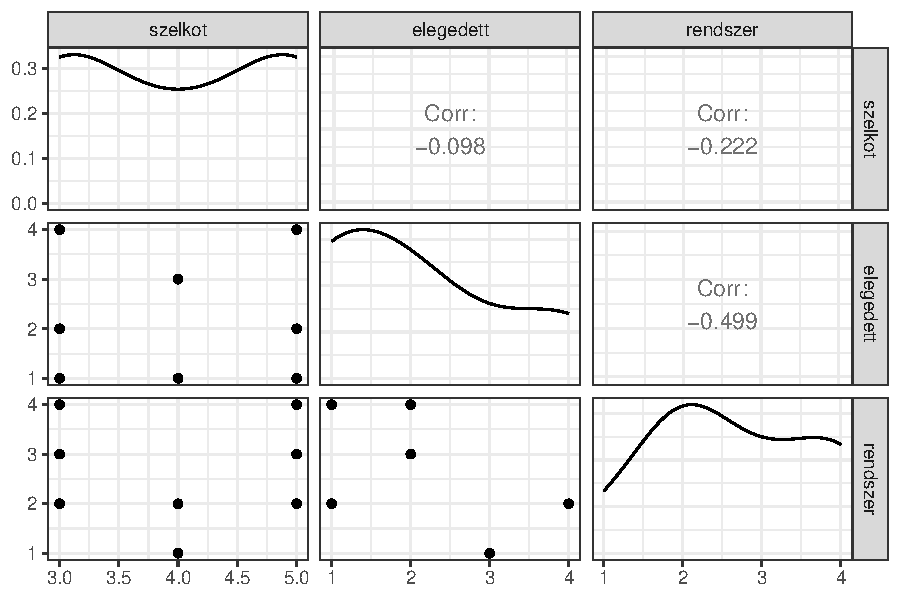
\includegraphics{./sec_tobbvaltozos_variancia_files/figure-pdf/unnamed-chunk-19-1.pdf}

}

\end{figure}

\begin{figure}[H]

{\centering 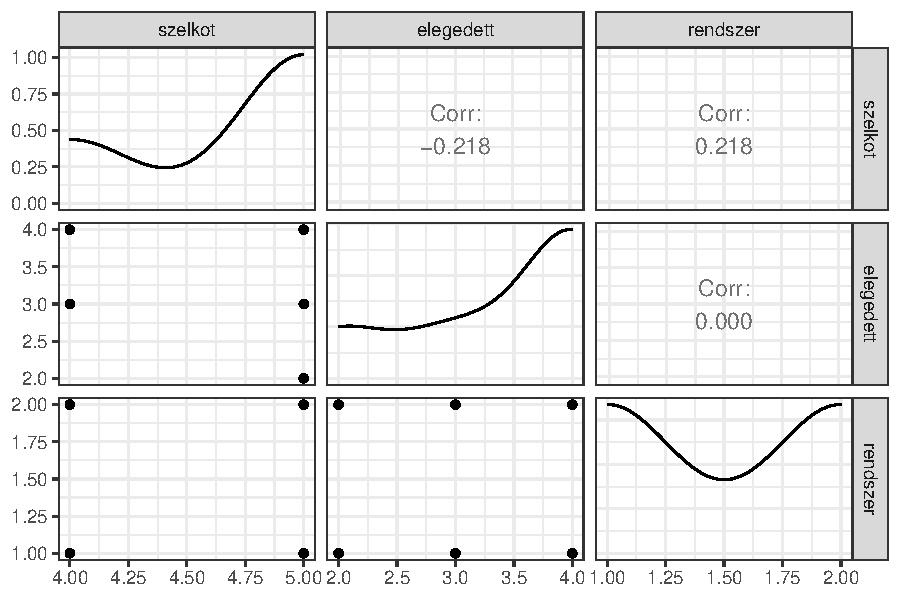
\includegraphics{./sec_tobbvaltozos_variancia_files/figure-pdf/unnamed-chunk-19-2.pdf}

}

\end{figure}

\begin{figure}[H]

{\centering 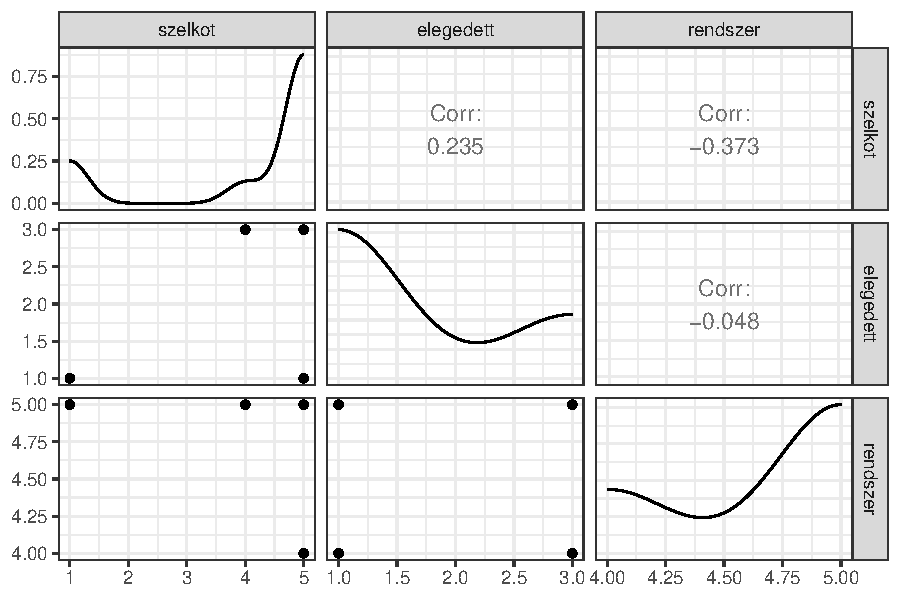
\includegraphics{./sec_tobbvaltozos_variancia_files/figure-pdf/unnamed-chunk-19-3.pdf}

}

\end{figure}

A fenti ábrák megkérdőjelezik a páronkénti lineáris kapcsolatok
létezését.

\begin{itemize}
\tightlist
\item
  \textbf{A varianciák homogenitása.} A Levene-próba használható a
  csoportok közötti varianciák egyenlőségének tesztelésére. A
  Levene-próba nem szignifikáns értékei a varianciák homogenitását
  támogatják.
\end{itemize}

Az egyszempontos MANOVA mindegyik függő változó esetében azt
feltételezi, hogy a csoportok között egyenlők a varianciák.

\begin{Shaded}
\begin{Highlighting}[]
\NormalTok{DescTools}\SpecialCharTok{::}\FunctionTok{LeveneTest}\NormalTok{(szelkot }\SpecialCharTok{\textasciitilde{}}\NormalTok{ SUE, }\AttributeTok{data =}\NormalTok{ vezetes)}
\CommentTok{\#\textgreater{} Levene\textquotesingle{}s Test for Homogeneity of Variance (center =...}
\CommentTok{\#\textgreater{}       Df F value Pr(\textgreater{}F)}
\CommentTok{\#\textgreater{} group  2  0.9755 0.3899}
\CommentTok{\#\textgreater{}       27}
\NormalTok{DescTools}\SpecialCharTok{::}\FunctionTok{LeveneTest}\NormalTok{(elegedett }\SpecialCharTok{\textasciitilde{}}\NormalTok{ SUE, }\AttributeTok{data =}\NormalTok{ vezetes)}
\CommentTok{\#\textgreater{} Levene\textquotesingle{}s Test for Homogeneity of Variance (center =...}
\CommentTok{\#\textgreater{}       Df F value Pr(\textgreater{}F)}
\CommentTok{\#\textgreater{} group  2  0.4112  0.667}
\CommentTok{\#\textgreater{}       27}
\NormalTok{DescTools}\SpecialCharTok{::}\FunctionTok{LeveneTest}\NormalTok{(rendszer }\SpecialCharTok{\textasciitilde{}}\NormalTok{ SUE, }\AttributeTok{data =}\NormalTok{ vezetes)}
\CommentTok{\#\textgreater{} Levene\textquotesingle{}s Test for Homogeneity of Variance (center =...}
\CommentTok{\#\textgreater{}       Df F value   Pr(\textgreater{}F)   }
\CommentTok{\#\textgreater{} group  2     5.6 0.009238 **}
\CommentTok{\#\textgreater{}       27                    }
\CommentTok{\#\textgreater{} {-}{-}{-}}
\CommentTok{\#\textgreater{} Signif. codes:  }
\CommentTok{\#\textgreater{} 0 \textquotesingle{}***\textquotesingle{} 0.001 \textquotesingle{}**\textquotesingle{} 0.01 \textquotesingle{}*\textquotesingle{} 0.05 \textquotesingle{}.\textquotesingle{} 0.1 \textquotesingle{} \textquotesingle{} 1}
\end{Highlighting}
\end{Shaded}

Látható, hogy a szóráshomogenitás a \texttt{rendszer} változó
kivételével teljesül.

\begin{itemize}
\tightlist
\item
  \textbf{Variancia-kovariancia mátrixok homogenitása.} A BoxM-próba
  használható a csoportok közötti kovariancia egyenlőségének
  ellenőrzésére. Ez egyenértékű a variancia többváltozós
  homogenitásával. Ez a teszt rendkívül érzékenynek tekinthető. Ezért
  ennek a tesztnek a szignifikanciáját alfa = 0,001 értéknél határozzuk
  meg. A \texttt{\{biotools\}} csomag megvalósított \texttt{boxM()}
  függvényét használhatjuk.
\end{itemize}

\begin{Shaded}
\begin{Highlighting}[]
\NormalTok{biotools}\SpecialCharTok{::}\FunctionTok{boxM}\NormalTok{(}\AttributeTok{data =}\NormalTok{ vezetes[}\FunctionTok{c}\NormalTok{(}\StringTok{"szelkot"}\NormalTok{, }\StringTok{"elegedett"}\NormalTok{, }\StringTok{"rendszer"}\NormalTok{)],}
    \AttributeTok{grouping =}\NormalTok{ vezetes}\SpecialCharTok{$}\NormalTok{SUE)}
\CommentTok{\#\textgreater{} }
\CommentTok{\#\textgreater{}  Box\textquotesingle{}s M{-}test for Homogeneity of Covariance}
\CommentTok{\#\textgreater{}  Matrices}
\CommentTok{\#\textgreater{} }
\CommentTok{\#\textgreater{} data:  vezetes[c("szelkot", "elegedett", "rendszer")]}
\CommentTok{\#\textgreater{} Chi{-}Sq (approx.) = 19.607, df = 12, p{-}value =}
\CommentTok{\#\textgreater{} 0.0749}
\end{Highlighting}
\end{Shaded}

A teszt statisztikailag nem szignifikáns (azaz p \textgreater{} 0,001),
tehát az adatok nem sértették meg a variancia-kovariancia mátrixok
homogenitásának feltételezését.

Kiegyensúlyozott a csoportelemszámok esetén nem probléma a
variancia-kovariancia mátrixok homogenitásának megsértése miatt, de
kiegyensúlyozatlan kialakításnál már problémás lehet.

\bookmarksetup{startatroot}

\hypertarget{sec-logisztikus-regresszio}{%
\chapter{Logisztikus regresszió}\label{sec-logisztikus-regresszio}}

A logisztikus regresszió céljait tekintve megegyezik a diszkriminancia
elemzéssel, de sokkal robusztusabb, azaz kevesebb alkalmazási
feltétellel rendelkezik. Használható a logisztikus regresszió akkor is,
ha a független változók között kategorikus változók is előfordulnak,
illetve a normalitásra és homoszkedaszticitásra vonatkozó feltétel
megsértésre sem érzékeny a módszer.

JÖN.

\bookmarksetup{startatroot}

\hypertarget{sec-tobbdimenzios-skalazas}{%
\chapter{Többdimenziós skálázás}\label{sec-tobbdimenzios-skalazas}}

JÖN.

\appendix
\addcontentsline{toc}{part}{Függelék}

\hypertarget{sec-elerheto-videok}{%
\chapter{Elérhető videók}\label{sec-elerheto-videok}}

\begin{itemize}
\item
  Alapozo jamovi és R videók

  \begin{itemize}
  \tightlist
  \item
    \href{https://www.youtube.com/watch?v=sZummF3Sd90\&list=PLnmeQHnHYqv5_FoVOvX9tqE90EqoOW01o}{Jamovi
    a gyakorlatban}
  \item
    \href{https://www.youtube.com/watch?v=UBeiIKzE8VA\&list=PLnmeQHnHYqv6ENGrdTXiE9YJrvHuxH2C9}{R
    a gyakorlatban}
  \end{itemize}
\item
  Jamovi tutorial videók az összes tanult eljáráshoz

  \begin{itemize}
  \tightlist
  \item
    \href{https://www.youtube.com/@datalabcc/videos}{datalab.cc}
  \item
    \href{https://www.youtube.com/@AlexanderSwan/videos}{Alexander Swan}
  \end{itemize}
\item
  Lineáris regresszió

  \begin{itemize}
  \tightlist
  \item
    \href{https://www.youtube.com/watch?v=m88h75F3Rl8}{The linear
    regression model}
  \item
    \href{https://www.youtube.com/watch?v=nk2CQITm_eo}{Linear
    Regression, Clearly Explained}
  \item
    \href{https://www.youtube.com/watch?v=2AQKmw14mHM}{R-squared,
    Clearly Explained}
  \item
    \href{https://www.youtube.com/watch?v=rUMWjRE8L1U}{Simple linear
    regression in Jamovi}
  \end{itemize}
\item
  Főkomponens elemzés

  \begin{itemize}
  \tightlist
  \item
    \href{https://www.youtube.com/watch?v=g-Hb26agBFg}{Principal
    Component Analysis (PCA)}
  \end{itemize}
\item
  Klaszterelemzés

  \begin{itemize}
  \tightlist
  \item
    \href{https://www.youtube.com/watch?v=ijUMKMC4f9I}{Flat and
    Hierarchical Clustering \textbar{} The Dendrogram Explained}
  \item
    \href{https://www.youtube.com/watch?v=YIGtalP1mv0}{K Means
    Clustering: Pros and Cons of K Means Clustering}
  \item
    \href{https://www.youtube.com/watch?v=TnFfAQpq0o4}{Hierarchical
    Cluster analysis in Jamovi}
  \item
    \href{https://www.youtube.com/watch?v=wW7TNlam77A}{K Means Cluster
    analysis in Jamovi}
  \end{itemize}
\item
  Többszempontos varianciaelemzés

  \begin{itemize}
  \tightlist
  \item
    \href{https://www.youtube.com/watch?v=pECfK5IfB_o}{One Way ANOVA
    Post hoc test in Jamovi}
  \item
    \href{https://www.youtube.com/watch?v=O6BiwVRj3BQ}{One Way Repeated
    Measure ANOVA Repeated Measure ANOVA Within Subject ANOVA in Jamovi}
  \item
    \href{https://www.youtube.com/watch?v=l6ClJFgxNXs}{Two Way ANOVA
    Post hoc test in Jamovi}
  \item
    \href{https://www.youtube.com/watch?v=WW8ALE6x3uQ}{Three Way ANOVA
    Post hoc test in Jamovi}
  \end{itemize}
\end{itemize}

\hypertarget{sec-adatbazisok}{%
\chapter{Adatbázisok}\label{sec-adatbazisok}}

Jelen jegyzetben ``könyv'' alatt a következőt értjük:

\begin{itemize}
\tightlist
\item
  Münnich Ákos, Nagy Ágnes, Abari Kálmán. \emph{Többváltozós statisztika
  pszichológus hallgatók számára.} Bölcsész Konzorcium, Debrecen, 2006.
  (http://psycho.unideb.hu/statisztika) ISBN 963 9704 04 0
\end{itemize}

\hypertarget{megbuxedzhatuxf3suxe1g-elemzuxe9s}{%
\section{Megbízhatóság
elemzés}\label{megbuxedzhatuxf3suxe1g-elemzuxe9s}}

\begin{itemize}
\item
  \texttt{megbizhatosag\_tantargyak.xlsx} - fiktív adatbázis 9 tanuló
  iskolai jegyeivel (Münnich és mtsai. (2006), 2.2. táblázat)

  \begin{itemize}
  \item
    Az adatbázis szerkezete:

    \begin{itemize}
    \tightlist
    \item
      \texttt{matek} - matematika érdemjegy (numerikus: 1-5)
    \item
      \texttt{fizika} - fizika érdemjegy (numerikus: 1-5)
    \item
      \texttt{informatika} - informatika érdemjegy (numerikus: 1-5)
    \item
      \texttt{kemia} - kémia érdemjegy (numerikus: 1-5)
    \end{itemize}
  \item
    Kapcsolódó állományok:

    \begin{itemize}
    \tightlist
    \item
      \texttt{megbizhatosag\_tantargyak.omv} - megbízhatóság elemzés
      jamovi-ban
    \end{itemize}
  \end{itemize}
\end{itemize}

\hypertarget{tuxf6bbvuxe1ltozuxf3s-varianciaelemzuxe9s}{%
\section{Többváltozós
varianciaelemzés}\label{tuxf6bbvuxe1ltozuxf3s-varianciaelemzuxe9s}}

\begin{itemize}
\item
  \texttt{manova\_vezetesi\_program.xlsx} - A szervezeti
  elkötelezettség, a szervezeti kultúra és az elégedettség eltér a
  vállalat 3 különböző vezetési irányelvét valló egységében? Az
  adatbázis Sajtos és Mitev (2007, o. 332) könyvéből származik.\\
  Egy vállalat menedzsmentje szeretné megvizsgálni különböző vezetési
  programok hatását, ezért három különböző vezetési programot vezetett
  be három különböző stratégiai üzleti egységben (SÜE). Az első SÜE-ben
  bevezetett program az egyenlőséget és az individualizmust
  hangsúlyozta. A második SÜE-ben az egyenlőséget és a csoportmunkát
  helyzeték középpontba. A harmadik SÜE-ben a bevezetett program egy
  nagyon hierarchikus vezetési elvet alkalmazott. Később mindhárom SÜE
  dolgozóinak körében felmérést végeztek, és a kérdések között szerepelt
  a szervezettel való elkötelezettség mértéke (\texttt{szelkot}), a
  szervezettel való elégedettség nagysága (\texttt{elegedett}), illetve
  a rendszer egalitárius vagy tekintélyelvű (autokrata) jellege
  (\texttt{rendszer}).

  \begin{itemize}
  \item
    Az adatbázis szerkezete:

    \begin{itemize}
    \tightlist
    \item
      \texttt{SUE} - a három különböző vezetési irányelvet követő
      stratégiai üzleti egység (nominális: 1-3)
    \item
      \texttt{szelkot} - szervezet elkötelezettség mértéke (likert: 1-5)
    \item
      \texttt{elegedett} - szervezettel való elégedettség (likert: 1-5)
    \item
      \texttt{rendszer} - szervezet tekintélyelvű jellege (likert: 1-5)
    \end{itemize}
  \item
    Kapcsolódó állományok:

    \begin{itemize}
    \tightlist
    \item
      \texttt{manova\_vezetesi\_program.omv} - Többváltozós
      varianciaelemzés jamovi-ban
    \end{itemize}
  \end{itemize}
\end{itemize}

\hypertarget{diszkriminancia-elemzuxe9s}{%
\section{Diszkriminancia elemzés}\label{diszkriminancia-elemzuxe9s}}

\begin{itemize}
\item
  \texttt{diszkriminancia\_alkalmassag.xlsx} - szalagmunkások adatai
  (Münnich és mtsai. (2006), 4.1. táblázat)

  \begin{itemize}
  \item
    Az adatbázis szerkezete:

    \begin{itemize}
    \tightlist
    \item
      \texttt{bevalt} - a munkás beválásával kapcsolatos információ:
      bevált? (nominális: ``igen'', ``nem'')
    \item
      \texttt{figyelem} - a munkás figyelmi képessége (likert: 1-7, a
      magasabb érték jobb képességeket jelent)
    \item
      \texttt{monotonia\_tures} - a munkás monotónia tűrése (likert:
      1-7, a magasabb érték jobb képességeket jelent)
    \end{itemize}
  \end{itemize}
\item
  \texttt{diszkriminancia\_baleset.xlsx} - mely tényezők járulnak hozzá
  a balesetekhez (Münnich és mtsai. (2006), 4.11. R-forráskód)

  \begin{itemize}
  \item
    Az adatbázis szerkezete:

    \begin{itemize}
    \tightlist
    \item
      \texttt{baleset} - volt már balesete a személynek vagy sem
      (nominális ``nem volt balesete'', ``volt baleste'')
    \item
      \texttt{megosztott} - megosztott figyelem (intervallum/arány)
    \item
      \texttt{pontossag} - a figyelem pontossága (intervallum/arány)
    \item
      \texttt{kockazat} - kockázatvállalási hajlandóság
      (intervallum/arány)
    \item
      \texttt{eszleles} - észlelés gyorsasága (intervallum/arány)
    \end{itemize}
  \end{itemize}
\item
  \texttt{diszkriminancia\_depresszio.xlsx} - a postpartum depresszió
  pszichés és szociális háttere (Münnich és mtsai. (2006), 4.16.
  R-forráskód)

  \begin{itemize}
  \item
    Az adatbázis szerkezete:

    \begin{itemize}
    \tightlist
    \item
      \texttt{ppdepresszio} - szülés utáni depresszió jelenléte
      (nominális: ``nincs depresszió'', ``van depresszió'')
    \item
      \texttt{szeretet} - a személyek mennyire érzik, hogy a szüleik
      szeretik őket (intervallum/arány)
    \item
      \texttt{tulvedes} - mennyire hajlamosak arra a személyek, hogy
      túlságosan is burokban tartsák, túlvédjék gyerekeiket
      (intervallum/arány)
    \item
      \texttt{kor} - életkor (intervallum/arány)
    \item
      \texttt{iskola} - az elvégzett iskolai osztályok száma
      (intervallum/arány)
    \end{itemize}
  \end{itemize}
\item
  \texttt{diszkriminancia\_pszichoszomatika.xlsx} - a pszichoszomatikus
  megbetegedéseket vizsgálata (Münnich és mtsai. (2006), 4.21.
  R-forráskód)

  \begin{itemize}
  \tightlist
  \item
    Az adatbázis szerkezete:

    \begin{itemize}
    \tightlist
    \item
      \texttt{pszichoszomatika} - van valamilyen pszichoszomatikus
      megbetegedése a személynek? (nominális: ``szichoszomatikus
      megbetegedése van'', '' egészséges'')
    \item
      \texttt{stressz} - a személyt ért stressz mértéke
      (intervallum/arány)
    \item
      \texttt{szorongas} - a szorongási szintje (intervallum/arány)
    \item
      \texttt{coping} - a megküzdési stratégiáinak hatékonysága
      (intervallum/arány)
    \end{itemize}
  \end{itemize}
\item
  \texttt{diszkriminancia\_bio.xlsx} - kik vásárolnak bio termékeket
  (Münnich és mtsai. (2006), 4.26. R-forráskód)

  \begin{itemize}
  \item
    Az adatbázis szerkezete:

    \begin{itemize}
    \tightlist
    \item
      \texttt{vasarlas} - a biotermékek vásárlásának gyakorisága
      (ordinális: ``soha nem vesz'', ``időnként vesz'', ``gyakran
      vesz'')
    \item
      \texttt{ertek} - minél nagyobb pontszámot kap a skálán, annál
      jobban értékeli a személy a bio termékeket (intervallum/arány)
    \item
      \texttt{attitud} - a magasabb értékek kedvezőbb atttitűdöt jelez a
      biotermékek iránt (intervallum/arány)
    \item
      \texttt{fizetes} - a személy fizetésének nagysága
      (intervallum/arány)
    \item
      \texttt{kor} - a személy életkora(intervallum/arány)
    \end{itemize}
  \end{itemize}
\item
  \texttt{diszkriminancia\_vezetesi\_program.xlsx} - A szervezeti
  elkötelezettség, a szervezeti kultúra és az elégedettség alapján
  szétválasztható a vállalat 3 különböző vezetési irányelvét valló
  egysége? Az adatbázis Sajtos és Mitev (2007, o. 332) könyvéből
  származik.\\
  Egy vállalat menedzsmentje szeretné megvizsgálni különböző vezetési
  programok hatását, ezért három különböző vezetési programot vezetett
  be három különböző stratégiai üzleti egységben (SÜE). Az első SÜE-ben
  bevezetett program az egyenlőséget és az individualizmust
  hangsúlyozta. A második SÜE-ben az egyenlőséget és a csoportmunkát
  helyzeték középpontba. A harmadik SÜE-ben a bevezetett program egy
  nagyon hierarchikus vezetési elvet alkalmazott. Később mindhárom SÜE
  dolgozóinak körében felmérést végeztek, és a kérdések között szerepelt
  a szervezettel való elkötelezettség mértéke (\texttt{szelkot}), a
  szervezettel való elégedettség nagysága (\texttt{elegedett}), illetve
  a rendszer egalitárius vagy tekintélyelvű (autokrata) jellege
  (\texttt{rendszer}).

  \begin{itemize}
  \tightlist
  \item
    Az adatbázis szerkezete:

    \begin{itemize}
    \tightlist
    \item
      \texttt{SUE} - a három különböző vezetési irányelvet követő
      stratégiai üzleti egység (nominális: 1-3)
    \item
      \texttt{szelkot} - szervezet elkötelezettség mértéke (likert: 1-5)
    \item
      \texttt{elegedett} - szervezettel való elégedettség (likert: 1-5)
    \item
      \texttt{rendszer} - szervezet tekintélyelvű jellege (likert: 1-5)
    \end{itemize}
  \item
    Kapcsolódó állományok:

    \begin{itemize}
    \tightlist
    \item
      \texttt{diszkriminancia\_vezetesi\_program.omv} - diszkriminancia
      elemzés jamovi-ban
    \end{itemize}
  \end{itemize}
\end{itemize}

\hypertarget{lineuxe1ris-regressziuxf3}{%
\section{Lineáris regresszió}\label{lineuxe1ris-regressziuxf3}}

\begin{itemize}
\tightlist
\item
  \texttt{lin\_reg\_fizetes\_elegedettseg\_01.omv} - konstans
  oszlopokkal nem tudunk számolni (Münnich és mtsai. (2006) 1.1/A
  táblázat)
\item
  \texttt{lin\_reg\_fizetes\_elegedettseg\_02.omv}- az adatpontok szinte
  tökéletesen az egyenesre illeszkednek (Münnich és mtsai. (2006) 1.1/B
  táblázat)
\item
  \texttt{lin\_reg\_kapcsolatok\_01.omv} - nem szisztematikus kapcsolat
  két változó között (Münnich és mtsai. (2006) 1.5. R-forráskód)
\item
  \texttt{lin\_reg\_kapcsolatok\_02.omv} - szisztematikus
  (függvényszerű) kapcsolat két változó között (Münnich és mtsai. (2006)
  1.6. R-forráskód)
\item
  \texttt{lin\_reg\_kapcsolatok\_03.omv} - szisztematikus
  (függvényszerű) kapcsolat két változó között (Münnich és mtsai. (2006)
  1.7. R-forráskód)
\item
  \texttt{lin\_reg\_kapcsolatok\_04.omv} - szisztematikus
  (függvényszerű) kapcsolat két változó között (Münnich és mtsai. (2006)
  1.8. R-forráskód)
\item
  \texttt{lin\_reg\_kapcsolatok\_05.omv} - szisztematikus
  (függvényszerű) kapcsolat két változó között (Münnich és mtsai. (2006)
  1.9. R-forráskód)
\item
  \texttt{lin\_reg\_elegedttseg.omv} - a fizetés és a munkahellyel való
  elégedettség pontdiagramja, egyszerű lineáris regresszió (Münnich és
  mtsai. (2006) 1.10 R-forráskód)
\item
  \texttt{lin\_reg\_fizetes\_eletkor\_eledettseg\_01.omv} - többszörös
  lineáris regresszió, 2 numerikus magyarázó változó (Münnich és mtsai.
  (2006) 1.2. táblázat)
\item
  \texttt{lin\_reg\_intelligencia\_testmagassag\_eletkor\_01.omv} -
  többszörös lineáris regresszió, 2 numerikus magyarázó változó,
  parciális korreláció magyarázata

  \begin{itemize}
  \tightlist
  \item
    minél magasabb valaki, annál intelligensebb
  \item
    ha bevonjuk az életkor változót, akkor eltűnik az intelligencia és a
    testmagasság közötti kapcsolat
  \end{itemize}
\item
  \texttt{lin\_tizproba.omv} - többszörös lineáris regresszió, a legjobb
  modell keresése, sok numerikus magyarázó változó
\item
  \texttt{lin\_college\_success\_02.omv} - többszörös lineáris
  regresszió, sok numerikus magyarázó változó, GPA a függő változó, mi
  magyarázza az egyetemi teljesítményt
\item
  \texttt{lin\_reg\_elegedttseg\_02.omv} - A férfiak vagy a nők
  elégedettebbek a munkahelyükkel? (Münnich és mtsai. (2006) 1.6.3
  probléma), egyetlen kategorikus magyarázó változó 2 értékkel (nem:
  férfi, nő)

  \begin{itemize}
  \tightlist
  \item
    kapcsolat a kétmintás t-próbával
  \end{itemize}
\item
  \texttt{lin\_reg\_magassag\_hajhossz\_nem\_01.omv} - többszörös
  lineáris regresszió, parciális korreláció 1 numerikus és 1 kategorikus
  változóval (Münnich és mtsai. (2006) 1.2. táblázat)

  \begin{itemize}
  \tightlist
  \item
    a testmagasság és a hajhossz között kapcsolat van
  \item
    ha a személyek nemét is figyelembe vesszük, egyáltalán nincs
    kapcsolat a testmagasság és a hajhosszúság között
  \end{itemize}
\item
  \texttt{lin\_auction.omv} - többszörös lineáris regresszió, Simpson
  paradoxon, párhuzamos regresszió, majd interakció bevonása.
\end{itemize}

\hypertarget{fux151komponens-elemzuxe9s}{%
\section{Főkomponens elemzés}\label{fux151komponens-elemzuxe9s}}

\begin{itemize}
\tightlist
\item
  \texttt{fokomp\_elemzes\_tantargyak.omv} - 1 főkomponens létrehozása
  (Münnich és mtsai. (2006) 2.2. táblázat)
\item
  \texttt{fokomp\_real\_targyak.omv} - példa kidolgozása, 1
  főkomponens(Münnich és mtsai. (2006) 2.5.1 Probléma)
\item
  \texttt{fokomp\_kerdoivtervezet.omv} - példa kidolgozása (Münnich és
  mtsai. (2006) 2.5.2 Probléma)
\item
  \texttt{fokomp\_munkahelyi\_tolarencia.omv} - példa kidolgozása
  (Münnich és mtsai. (2006) 2.5.3 Probléma)
\item
  \texttt{fokomp\_munkahelyi\_elegedettseg.omv} - példa kidolgozása
  (Münnich és mtsai. (2006) 2.5.4 Probléma)
\end{itemize}

\hypertarget{faktorelemzuxe9s}{%
\section{Faktorelemzés}\label{faktorelemzuxe9s}}

\begin{itemize}
\tightlist
\item
  \texttt{faktor\_szorongas.omv} - példa (Münnich és mtsai. (2006) 3.1.
  R-forráskód)
\item
  \texttt{faktor\_real\_human\_targyak.omv} - példa (Münnich és mtsai.
  (2006) 3.9. R-forráskód)
\item
  \texttt{faktor\_bigfive.omv} - példa (Münnich és mtsai. (2006) 3.21.
  R-forráskód)
\item
  \texttt{faktor\_kockazat.omv} - példa (Münnich és mtsai. (2006) 3.7.4
  Probléma)
\item
  \texttt{faktor\_fogkrem.omv} - példa (Malhotra és Simon (2008) 617.
  oldal)
\end{itemize}

\hypertarget{feltuxe1ruxf3-faktorelemzuxe9s}{%
\section{Feltáró faktorelemzés}\label{feltuxe1ruxf3-faktorelemzuxe9s}}

\begin{itemize}
\item
  \texttt{faktor\_fogkrem.xlsx} - A kutató arra volt kíváncsi, milyen
  előnyöket keresnek a fogyasztók a fogrémvásárlásnál. Egy 30 fős mintán
  a válaszadókat arra kérték, hogy jelezzék, mennyire értenek egyet a
  következő állításokkal (1 = egyáltalán nem ért egyet; 7 = teljes
  mértékben egyetért)

  \begin{itemize}
  \item
    Az adatbázis szerkezete:

    \begin{itemize}
    \tightlist
    \item
      \texttt{sorszam}: válaszadó sorszáma (id)
    \item
      \texttt{v1}: Fontos, hogy olyan fogkrémet vásároljak, amellyel
      megelőzhető a fogszuvasodás. (likert: 1-7)
    \item
      \texttt{v2}: Az olyan fogkrémeket szeretem, amely fényessé teszi a
      fogaimat. (likert: 1-7)
    \item
      \texttt{v3}: Egy fogkrémnek erősítenie kell a fogínyt. (likert:
      1-7)
    \item
      \texttt{v4}: Az olyan fogkrémeket szeretem, amely friss leheletet
      biztosít. (likert: 1-7)
    \item
      \texttt{v5}: A fog romlásának megelőzése számomra nem fontos
      elvárás. (likert: 1-7)
    \item
      \texttt{v6}: A legfontosabb szempont a fogkrém vásárlásánál a szép
      fog. (likert: 1-7)
    \end{itemize}
  \item
    Kapcsolódó állományok:

    \begin{itemize}
    \tightlist
    \item
      \texttt{efa\_fogkrem.omv} - Feltáró faktorelemzés jamovi-ban
    \end{itemize}
  \end{itemize}
\end{itemize}

\hypertarget{irodalomjegyzuxe9k}{%
\chapter{Irodalomjegyzék}\label{irodalomjegyzuxe9k}}

\hypertarget{refs}{}
\begin{CSLReferences}{1}{0}
\leavevmode\vadjust pre{\hypertarget{ref-CarverScheier2006}{}}%
Carver, C. S. és Scheier, M. F. (2006). \emph{Személyiségpszichológia}.
Osiris Kiadó.

\leavevmode\vadjust pre{\hypertarget{ref-Csallner2015}{}}%
Csallner, A. E. (2015). \emph{Bevezetés az SPSS statisztikai
programcsomag használatába}.
\url{http://www.jgypk.hu/tamop15e/tananyag_html/spss/index.html}

\leavevmode\vadjust pre{\hypertarget{ref-Horn1965}{}}%
Horn, J. L. (1965). A rationale and test for the number of factors in
factor analysis. \emph{Psychometrika}, \emph{30}, 179--185.
\url{https://doi.org/10.1007/BF02289447}

\leavevmode\vadjust pre{\hypertarget{ref-Karasz2022}{}}%
Kárász, J. T., Nagy, O. N., Széll, K. és Takács, S. (2022).
Cronbach-alfa: vele vagy nélküle? \emph{Magyar Pszichológiai Szemle},
\emph{77}, 81--98. \url{https://doi.org/10.1556/0016.2022.00004}

\leavevmode\vadjust pre{\hypertarget{ref-KetskemetyIzso2005}{}}%
Ketskeméty, L. és Izsó, L. (2005). \emph{Bevezetés az SPSS
programrendszerbe - Módszertani útmutató és feladatgyűjtemény
statisztikai elemzésekhez}. ELTE Eötvös Kiadó.

\leavevmode\vadjust pre{\hypertarget{ref-MalhotraSimon2008}{}}%
Malhotra, N. K. és Simon, J. (2008). \emph{Marketingkutatás}. Akadémiai
Kiadó.

\leavevmode\vadjust pre{\hypertarget{ref-Malkewitz2023}{}}%
Malkewitz, C. P., Schwall, P., Meesters, C. és Hardt, J. (2023).
Estimating reliability: A comparison of Cronbach's α, McDonald's ωt and
the greatest lower bound. \emph{Social Sciences \& Humanities Open},
\emph{7}, 100368. \url{https://doi.org/10.1016/j.ssaho.2022.100368}

\leavevmode\vadjust pre{\hypertarget{ref-Moksony2006}{}}%
Moksony, F. (2006). \emph{Gondolatok és adatok. Társadalomtudományi
elméletek empirikus ellenőrzése}. Aula Kiadó.

\leavevmode\vadjust pre{\hypertarget{ref-MunnichNagyAbari2006}{}}%
Münnich, Á., Nagy, Á. és Abari, K. (2006). \emph{Többváltozós
statisztika pszichológus hallgatók számára}. Bölcsész Konzorcium.
\url{http://psycho.unideb.hu/statisztika}

\leavevmode\vadjust pre{\hypertarget{ref-Nagybanyai2006}{}}%
Nagy, O. N. (2006). A pszichológiai tesztek reliabilitása. In S. Rózsa,
O. N. Nagy, és A. Oláh (Szerk.), \emph{A pszichológiai mérés alapjai.
Elmélet, módszer és gyakorlati alkalmazás}. Bölcsész Konzorcium.
\url{https://mek.oszk.hu/05500/05536/05536.pdf}

\leavevmode\vadjust pre{\hypertarget{ref-Rozsa2019}{}}%
Rózsa, S., Hupuczi, E., Martin, L., Birkás, B., Hartung, I., Hargitai,
R., Varga, J., Láng, A., Tiringer, I. és Kállai, J. (2019). A Tellegen
Abszorpciós Skála részletes pszichometriai elemzése. \emph{Mentálhigiéné
és Pszichoszomatika}, \emph{20}, 35--77.
\url{https://doi.org/10.1556/0406.20.2019.003}

\leavevmode\vadjust pre{\hypertarget{ref-SajtosMitev2007}{}}%
Sajtos, L. és Mitev, A. (2007). \emph{SPSS kutatási és adatelemzési
kézikönyv}. Alinea Kiadó.

\leavevmode\vadjust pre{\hypertarget{ref-SzekelyiBarna2002}{}}%
Székelyi, M. és Barna, I. (2002). \emph{Túlélőkészlet az SPSS-hez.
Többváltozós elemzési technikáról társadalomkutatók számára}. Typotex
Kiadó.

\leavevmode\vadjust pre{\hypertarget{ref-TakacsBev22017}{}}%
Takács, S. (2017). \emph{Bevezetés a matematikai statisztikába 2.
Többváltozós statisztikai módszerek}. Antarész Kiadó.

\leavevmode\vadjust pre{\hypertarget{ref-Varga2019}{}}%
Varga, A. (2019). \emph{Többváltozós statisztika dióhéjban:
Változó-orientált módszerek}. Pólya Kiadó.

\leavevmode\vadjust pre{\hypertarget{ref-Watkins2018}{}}%
Watkins, M. W. (2018). Exploratory Factor Analysis: A Guide to Best
Practice. \emph{Journal of Black Psychology}, \emph{44}, 219--246.
\url{https://doi.org/10.1177/0095798418771807}

\end{CSLReferences}



\backmatter
\printindex

\end{document}
